\RequirePackage[final]{graphicx}
\documentclass[draft]{thesis}

% Setting pdf metadata
\hypersetup{
  pdftitle = {Búsqueda de Supersimetría en eventos con un fóton, %
    jets y energía faltante con el detector ATLAS},
  pdfauthor = {Francisco Alonso},
  pdfkeywords = {SUSY} {GGM} {ATLAS} {LHC}
}

\tikzset{
  every picture/.append style={
    execute at begin picture={\deactivatequoting},
    execute at end picture={\activatequoting}
  }
}

\usepackage{hepparticles}

\let\sst=\scriptscriptstyle % Needed for some definitions (psi and eta prime, etc.) (EE)
\chardef\letterchar=11
\chardef\otherchar=12
\chardef\eolinechar=5
%
% +--------------------------------------------------------------------+
% |                                                                    |
% |  Useful symbols for use in or out of math mode                     |
% |                                                                    |
% +--------------------------------------------------------------------+
%
\def\ra{\ensuremath{\rightarrow}}%  "GOES TO" arrow.
\def\la{\ensuremath{\leftarrow}}%   "GETS" arrow.
\let\rarrow=\ra
\let\larrow=\la
\def\lapprox{\ensuremath{\sim\kern-1em\raise 0.65ex\hbox{$<$}}}%  Or use \lsim
\def\rapprox{\ensuremath{\sim\kern-1em\raise 0.65ex\hbox{$>$}}}%  and \rsim.
\def\gam{\ensuremath{\gamma}}
\def\rts {\ensuremath{\sqrt{s}}}
\def\stat{\mbox{$\;$(stat.)}}
\def\syst{\mbox{$\;$(syst.)}}
%
% +--------------------------------------------------------------------+
% |                                                                    |
% |  Particle-antiparticle pair notations                              |
% |                                                                    |
% +--------------------------------------------------------------------+
%
\def\antibar#1{\ensuremath{#1\bar{#1}}}
\def\tbar{\ensuremath{\bar{t}}}
\def\ttbar{\antibar{t}}
\def\bbar{\ensuremath{\bar{b}}}
\def\bbbar{\antibar{b}}
\def\cbar{\ensuremath{\bar{c}}}
\def\ccbar{\antibar{c}}
\def\sbar{\ensuremath{\bar{s}}}
\def\ssbar{\antibar{s}}
\def\ubar{\ensuremath{\bar{u}}}
\def\uubar{\antibar{u}}
\def\dbar{\ensuremath{\bar{d}}}
\def\ddbar{\antibar{d}}
\def\fbar{\ensuremath{\bar{f}}}
\def\ffbar{\antibar{f}}
\def\qbar{\ensuremath{\bar{q}}}
\def\qqbar{\antibar{q}}
\def\nbar{\ensuremath{\bar{\nu}}}
\def\nnbar{\antibar{\nu}}
%
% +--------------------------------------------------------------------+
% |                                                                    |
% |  e+e-, etc.                                                        |
% |                                                                    |
% +--------------------------------------------------------------------+
%
\def\ee{\ensuremath{e^+ e^-}}%
\def\epm{\ensuremath{e^{\pm}}}%
\def\epem{\ensuremath{e^+ e^-}}%
\def\mumu{\ensuremath{\mathrm{\mu^+ \mu^-}}}%
\def\tautau{\ensuremath{\mathrm{\tau^+ \tau^-}}}%
\let\muchless=\ll
\def\leplep{\ensuremath{\ell^+ \ell^-}}%
\def\lnu{\ensuremath{\ell \nu}}%
%
% +--------------------------------------------------------------------+
% |                                                                    |
% |  Useful Z0 type stuff    Gammas, asymmetries                       |
% |                                                                    |
% +--------------------------------------------------------------------+
\def\Zzero{\ensuremath{Z}}
\def\Zboson{\ensuremath{Z}}
\def\Wplus{\ensuremath{W^+}}
\def\Wminus{\ensuremath{W^-}}
\def\Wboson{\ensuremath{W}}%
\def\Wpm{\ensuremath{W^{\pm}}}%
\def\Wmp{\ensuremath{W^{\mp}}}%
\def\Zzv{\ensuremath{\Zzero^{\textstyle *}}}
\def\Abb{\ensuremath{A_{\bbbar}}}
\def\Acc{\ensuremath{A_{\ccbar}}}
\def\Aqq{\ensuremath{A_{\qqbar}}}
\def\Afb{\ensuremath{A_{{fb}}}} % Subscript italic not roman (EE)
\def\GZ{\ensuremath{\Gamma_{Z}}}
\def\GW{\ensuremath{\Gamma_{W}}}
\def\GH{\ensuremath{\Gamma_{H}}}
\def\GamHad{\ensuremath{\Gamma_{\mathrm{had}}}}
\def\Gbb{\ensuremath{\Gamma_{\bbbar}}}
\def\Rbb{\ensuremath{R_{\bbbar}}}
\def\Gcc{\ensuremath{\Gamma_{\ccbar}}}
\def\Gvis{\ensuremath{\Gamma_{\mathrm{vis}}}}
\def\Ginv{\ensuremath{\Gamma_{\mathrm{inv}}}}
%
% +--------------------------------------------------------------------+
% |                                                                    |
% |  QCD (Simplified all of these: no hbox, etc.) (EE)                 |
% |                                                                    |
% +--------------------------------------------------------------------+
%
\def\alphas{\ensuremath{\alpha_{\mathrm{S}}}} % Subscript roman not italic (EE)
\def\NF{\ensuremath{N_{\mathrm{F}}}}
\def\NC{\ensuremath{N_{\mathrm{C}}}}
\def\CF{\ensuremath{C_{\mathrm{F}}}}
\def\CA{\ensuremath{C_{\mathrm{A}}}}
\def\TF{\ensuremath{T_{\mathrm{F}}}}
\def\Lms{\ensuremath{\Lambda_{\overline{\mathrm{MS}}}}}
\def\Lmsfive{\ensuremath{\Lambda^{(5)}_{\overline{\mathrm{MS}}}}}
\def\KT{\ensuremath{k_{\perp}}}
%
% +--------------------------------------------------------------------+
% |                                                                    |
% |  CKM matrix                                                        |
% |                                                                    |
% +--------------------------------------------------------------------+
%
\def\Vcb{\ensuremath{\vert V_{cb} \vert}}
\def\Vub{\ensuremath{\vert V_{ub} \vert}}
\def\Vtd{\ensuremath{\vert V_{td} \vert}}
\def\Vts{\ensuremath{\vert V_{ts} \vert}}
\def\Vtb{\ensuremath{\vert V_{tb} \vert}}
\def\Vcs{\ensuremath{\vert V_{cs} \vert}}
\def\Vud{\ensuremath{\vert V_{ud} \vert}}
\def\Vus{\ensuremath{\vert V_{us} \vert}}
\def\Vcd{\ensuremath{\vert V_{cd} \vert}}
%
% +--------------------------------------------------------------------+
% |                                                                    |
% |  New particle stuff                                                |
% |                                                                    |
% +--------------------------------------------------------------------+
%
\def\Azero{\ensuremath{A^0}}%
\def\hzero{\ensuremath{h^0}}%
\def\Hzero{\ensuremath{H^0}}%
\def\Hboson{\ensuremath{H}}%
\def\Hplus{\ensuremath{H^+}}%
\def\Hminus{\ensuremath{H^-}}%
\def\Hpm{\ensuremath{H^{\pm}}}%
\def\Hmp{\ensuremath{H^{\mp}}}%
\def\susy#1{\ensuremath{\widetilde{#1}}}%
\def\ellell{\ensuremath{\mathrm{\ell^+ \ell^-}}}%
\def\ggino{\ensuremath{\mathchoice%
      {\displaystyle\raise.4ex\hbox{$\displaystyle\widetilde\chi$}}%
         {\textstyle\raise.4ex\hbox{$\textstyle\widetilde\chi$}}%
       {\scriptstyle\raise.3ex\hbox{$\scriptstyle\widetilde\chi$}}%
 {\scriptscriptstyle\raise.3ex\hbox{$\scriptscriptstyle\widetilde\chi$}}}}

\def\chinop{\ensuremath{\mathchoice%
      {\displaystyle\raise.4ex\hbox{$\displaystyle\widetilde\chi^+$}}%
         {\textstyle\raise.4ex\hbox{$\textstyle\widetilde\chi^+$}}%
       {\scriptstyle\raise.3ex\hbox{$\scriptstyle\widetilde\chi^+$}}%
 {\scriptscriptstyle\raise.3ex\hbox{$\scriptscriptstyle\widetilde\chi^+$}}}}
\def\chinom{\ensuremath{\mathchoice%
      {\displaystyle\raise.4ex\hbox{$\displaystyle\widetilde\chi^-$}}%
         {\textstyle\raise.4ex\hbox{$\textstyle\widetilde\chi^-$}}%
       {\scriptstyle\raise.3ex\hbox{$\scriptstyle\widetilde\chi^-$}}%
 {\scriptscriptstyle\raise.3ex\hbox{$\scriptscriptstyle\widetilde\chi^-$}}}}
\def\chinopm{\ensuremath{\mathchoice%
      {\displaystyle\raise.4ex\hbox{$\displaystyle\widetilde\chi^\pm$}}%
         {\textstyle\raise.4ex\hbox{$\textstyle\widetilde\chi^\pm$}}%
       {\scriptstyle\raise.3ex\hbox{$\scriptstyle\widetilde\chi^\pm$}}%
 {\scriptscriptstyle\raise.3ex\hbox{$\scriptscriptstyle\widetilde\chi^\pm$}}}}
\def\chinomp{\ensuremath{\mathchoice%
      {\displaystyle\raise.4ex\hbox{$\displaystyle\widetilde\chi^\mp$}}%
         {\textstyle\raise.4ex\hbox{$\textstyle\widetilde\chi^\mp$}}%
       {\scriptstyle\raise.3ex\hbox{$\scriptstyle\widetilde\chi^\mp$}}%
 {\scriptscriptstyle\raise.3ex\hbox{$\scriptscriptstyle\widetilde\chi^\mp$}}}}

\def\chinoonep{\ensuremath{\mathchoice%
      {\displaystyle\raise.4ex\hbox{$\displaystyle\widetilde\chi^+_1$}}%
         {\textstyle\raise.4ex\hbox{$\textstyle\widetilde\chi^+_1$}}%
       {\scriptstyle\raise.3ex\hbox{$\scriptstyle\widetilde\chi^+_1$}}%
 {\scriptscriptstyle\raise.3ex\hbox{$\scriptscriptstyle\widetilde\chi^+_1$}}}}
\def\chinoonem{\ensuremath{\mathchoice%
      {\displaystyle\raise.4ex\hbox{$\displaystyle\widetilde\chi^-_1$}}%
         {\textstyle\raise.4ex\hbox{$\textstyle\widetilde\chi^-_1$}}%
       {\scriptstyle\raise.3ex\hbox{$\scriptstyle\widetilde\chi^-_1$}}%
 {\scriptscriptstyle\raise.3ex\hbox{$\scriptscriptstyle\widetilde\chi^-_1$}}}}
\def\chinoonepm{\ensuremath{\mathchoice%
      {\displaystyle\raise.4ex\hbox{$\displaystyle\widetilde\chi^\pm_1$}}%
         {\textstyle\raise.4ex\hbox{$\textstyle\widetilde\chi^\pm_1$}}%
       {\scriptstyle\raise.3ex\hbox{$\scriptstyle\widetilde\chi^\pm_1$}}%
 {\scriptscriptstyle\raise.3ex\hbox{$\scriptscriptstyle\widetilde\chi^\pm_1$}}}}

\def\chinotwop{\ensuremath{\mathchoice%
      {\displaystyle\raise.4ex\hbox{$\displaystyle\widetilde\chi^+_2$}}%
         {\textstyle\raise.4ex\hbox{$\textstyle\widetilde\chi^+_2$}}%
       {\scriptstyle\raise.3ex\hbox{$\scriptstyle\widetilde\chi^+_2$}}%
 {\scriptscriptstyle\raise.3ex\hbox{$\scriptscriptstyle\widetilde\chi^+_2$}}}}
\def\chinotwom{\ensuremath{\mathchoice%
      {\displaystyle\raise.4ex\hbox{$\displaystyle\widetilde\chi^-_2$}}%
         {\textstyle\raise.4ex\hbox{$\textstyle\widetilde\chi^-_2$}}%
       {\scriptstyle\raise.3ex\hbox{$\scriptstyle\widetilde\chi^-_2$}}%
 {\scriptscriptstyle\raise.3ex\hbox{$\scriptscriptstyle\widetilde\chi^-_2$}}}}
\def\chinotwopm{\ensuremath{\mathchoice%
      {\displaystyle\raise.4ex\hbox{$\displaystyle\widetilde\chi^\pm_2$}}%
         {\textstyle\raise.4ex\hbox{$\textstyle\widetilde\chi^\pm_2$}}%
       {\scriptstyle\raise.3ex\hbox{$\scriptstyle\widetilde\chi^\pm_2$}}%
 {\scriptscriptstyle\raise.3ex\hbox{$\scriptscriptstyle\widetilde\chi^\pm_2$}}}}

\def\nino{\ensuremath{\mathchoice%
      {\displaystyle\raise.4ex\hbox{$\displaystyle\widetilde\chi^0$}}%
         {\textstyle\raise.4ex\hbox{$\textstyle\widetilde\chi^0$}}%
       {\scriptstyle\raise.3ex\hbox{$\scriptstyle\widetilde\chi^0$}}%
 {\scriptscriptstyle\raise.3ex\hbox{$\scriptscriptstyle\widetilde\chi^0$}}}}

\def\ninoone{\ensuremath{\mathchoice%
      {\displaystyle\raise.4ex\hbox{$\displaystyle\widetilde\chi^0_1$}}%
         {\textstyle\raise.4ex\hbox{$\textstyle\widetilde\chi^0_1$}}%
       {\scriptstyle\raise.3ex\hbox{$\scriptstyle\widetilde\chi^0_1$}}%
 {\scriptscriptstyle\raise.3ex\hbox{$\scriptscriptstyle\widetilde\chi^0_1$}}}}
\def\ninotwo{\ensuremath{\mathchoice%
      {\displaystyle\raise.4ex\hbox{$\displaystyle\widetilde\chi^0_2$}}%
         {\textstyle\raise.4ex\hbox{$\textstyle\widetilde\chi^0_2$}}%
       {\scriptstyle\raise.3ex\hbox{$\scriptstyle\widetilde\chi^0_2$}}%
 {\scriptscriptstyle\raise.3ex\hbox{$\scriptscriptstyle\widetilde\chi^0_2$}}}}
\def\ninothree{\ensuremath{\mathchoice%
      {\displaystyle\raise.4ex\hbox{$\displaystyle\widetilde\chi^0_3$}}%
         {\textstyle\raise.4ex\hbox{$\textstyle\widetilde\chi^0_3$}}%
       {\scriptstyle\raise.3ex\hbox{$\scriptstyle\widetilde\chi^0_3$}}%
 {\scriptscriptstyle\raise.3ex\hbox{$\scriptscriptstyle\widetilde\chi^0_3$}}}}
\def\ninofour{\ensuremath{\mathchoice%
      {\displaystyle\raise.4ex\hbox{$\displaystyle\widetilde\chi^0_4$}}%
         {\textstyle\raise.4ex\hbox{$\textstyle\widetilde\chi^0_4$}}%
       {\scriptstyle\raise.3ex\hbox{$\scriptstyle\widetilde\chi^0_4$}}%
 {\scriptscriptstyle\raise.3ex\hbox{$\scriptscriptstyle\widetilde\chi^0_4$}}}}

\def\gravino{\ensuremath{\widetilde{G}}}%
\def\Zprime{\ensuremath{Z^\prime}}
\def\Zstar{\ensuremath{Z^{*}}}
\def\squark{\ensuremath{\widetilde{q}}}
\def\squarkL{\ensuremath{\widetilde{q}_{\mathrm{L}}}} % Subscript roman not italic (EE)
\def\squarkR{\ensuremath{\widetilde{q}_{\mathrm{R}}}} % Subscript roman not italic (EE)
\def\gluino{\ensuremath{\widetilde{g}}}
\def\stop{\ensuremath{\widetilde{t}}}
\def\stopone{\ensuremath{\widetilde{t}_1}}
\def\stoptwo{\ensuremath{\widetilde{t}_2}}
\def\stopL{\ensuremath{\widetilde{t}_{\mathrm{L}}}} % Subscript roman not italic (EE)
\def\stopR{\ensuremath{\widetilde{t}_{\mathrm{R}}}} % Subscript roman not italic (EE)
\def\sbottom{\ensuremath{\widetilde{b}}}
\def\sbottomone{\ensuremath{\widetilde{b}_1}}
\def\sbottomtwo{\ensuremath{\widetilde{b}_2}}
\def\sbottomL{\ensuremath{\widetilde{b}_{\mathrm{L}}}} % Subscript roman not italic (EE)
\def\sbottomR{\ensuremath{\widetilde{b}_{\mathrm{R}}}} % Subscript roman not italic (EE)
\def\slepton{\ensuremath{\widetilde{\ell}}}
\def\sleptonL{\ensuremath{\widetilde{\ell}_{\mathrm{L}}}} % Subscript roman not italic (EE)
\def\sleptonR{\ensuremath{\widetilde{\ell}_{\mathrm{R}}}} % Subscript roman not italic (EE)
\def\sel{\ensuremath{\widetilde{e}}}
\def\selL{\ensuremath{\widetilde{e}_{\mathrm{L}}}} % Subscript roman not italic (EE)
\def\selR{\ensuremath{\widetilde{e}_{\mathrm{R}}}} % Subscript roman not italic (EE)
\def\smu{\ensuremath{\widetilde{\mu}}}
\def\smuL{\ensuremath{\widetilde{\mu}_{\mathrm{L}}}} % Subscript roman not italic (EE)
\def\smuR{\ensuremath{\widetilde{\mu}_{\mathrm{R}}}} % Subscript roman not italic (EE)
\def\stau{\ensuremath{\widetilde{\tau}}}
\def\stauL{\ensuremath{\widetilde{\tau}_{\mathrm{L}}}} % Subscript roman not italic (EE)
\def\stauR{\ensuremath{\widetilde{\tau}_{\mathrm{R}}}} % Subscript roman not italic (EE)
\def\stauone{\ensuremath{\widetilde{\tau}_1}}
\def\stautwo{\ensuremath{\widetilde{\tau}_2}}
\def\snu{\ensuremath{\widetilde{\nu}}}


%% \newcommand{\bino}{\HepGenSusyParticle{B}{}{}}
%% \newcommand{\winozero}{\HepSusyParticle{W}{}{0}}
%% \newcommand{\winop}{\HepSusyParticle{W}{}{+}}
%% \newcommand{\winom}{\HepSusyParticle{W}{}{-}}

\def\bino{\ensuremath{\widetilde{B}}}
\def\winozero{\ensuremath{\widetilde{W}^0}}
\def\winop{\ensuremath{\widetilde{W}^+}}
\def\winom{\ensuremath{\widetilde{W}^-}}
\def\zino{\ensuremath{\widetilde{Z}^0}}
\def\photino{\ensuremath{\tilde{\gamma}}}


%
% +--------------------------------------------------------------------+
% |                                                                    |
% |  pi, pi0, pi+, pi-, pi+-, eta, eta1, etc.                          |
% |                                                                    |
% +--------------------------------------------------------------------+
%
\let\pii=\pi
\def\pi{\ensuremath{\pii}}%
\def\pizero{\ensuremath{\pii^0}}%
\def\piplus{\ensuremath{\pii^+}}%
\def\piminus{\ensuremath{\pii^-}}%
\def\pipm{\ensuremath{\pii^{\pm}}}%
\def\pimp{\ensuremath{\pii^{\mp}}}%
\let\etaa=\eta
\def\eta{\ensuremath{\etaa}}%
\def\etaprime{\ensuremath{\eta^{\sst\prime}}}%

%
% +--------------------------------------------------------------------+
% |                                                                    |
% |  Useful things for proton-proton physics                           |
% |                                                                    |
% +--------------------------------------------------------------------+
%
\def\pt{\ensuremath{p_{\mathrm{T}}}} % Subscript roman not italic (EE)
\def\pT{\ensuremath{p_{\mathrm{T}}}} % Subscript roman not italic (EE)
\def\et{\ensuremath{E_{\mathrm{T}}}} % Subscript roman not italic (EE)
\def\eT{\ensuremath{E_{\mathrm{T}}}} % Subscript roman not italic (EE)
\def\ET{\ensuremath{E_{\mathrm{T}}}} % Subscript roman not italic (EE)
\def\HT{\ensuremath{H_{\mathrm{T}}}} % Subscript roman not italic (EE)
\def\ptsq{\ensuremath{p^2_{\mathrm{T}}}} % Fixed so it works correctly (EE)

\def\degr{\ensuremath{^\circ}} % Removed mbox - caused problems and not needed (EE)
\def\abseta{\ensuremath{|\eta|}}
\def\Hgg{\ensuremath{H\to\gamma\gamma}}
\def\mh{\ensuremath{m_h}}
\def\mW{\ensuremath{m_W}}
\def\mZ{\ensuremath{m_Z}}
\def\mH{\ensuremath{m_H}}
\def\mA{\ensuremath{m_A}}
\def\MET{\ensuremath{E_{\mathrm{T}}^{\mathrm{miss}}}} % Sub/superscript roman not italic (EE)
\def\met{\ensuremath{E_{\mathrm{T}}^{\mathrm{miss}}}} % Sub/superscript roman not italic (EE)
\def\etmiss{\ensuremath{E_{\mathrm{T}}^{\mathrm{miss}}}} % Sub/superscript roman not italic (EE)
\def\Wjj{\ensuremath{W \rightarrow jj}}
\def\tjjb{\ensuremath{t \rightarrow jjb}}
\def\Hbb{\ensuremath{H \rightarrow b\bar b}}
\def\Zmm{\ensuremath{Z \rightarrow \mu\mu}}
\def\Zee{\ensuremath{Z \rightarrow ee}}
\def\Zll{\ensuremath{Z \rightarrow \ell\ell}}
\def\Wln{\ensuremath{W \rightarrow \ell\nu}}
\def\Wen{\ensuremath{W \rightarrow e\nu}}
\def\Wmn{\ensuremath{W \rightarrow \mu\nu}}
\def\Hllll{\ensuremath{H \rightarrow ZZ^{(*)} \rightarrow \mu\mu\mu\mu}}
\def\Hmmmm{\ensuremath{H \rightarrow \mu\mu\mu\mu}}
\def\Heeee{\ensuremath{H \rightarrow eeee}}
\def\Amm{\ensuremath{A \rightarrow \mu\mu}}
\def\Ztau{\ensuremath{Z \rightarrow \tau\tau}}
\def\Wtau{\ensuremath{W \rightarrow \tau\nu}}
\def\Atau{\ensuremath{A \rightarrow \tau\tau}}
\def\Htau{\ensuremath{H \rightarrow \tau\tau}}
\def\begL{10$^{31}$~cm$^{-2}$~s$^{-1}$}
\def\lowL{10$^{33}$~cm$^{-2}$~s$^{-1}$}
\def\highL{10$^{34}$~cm$^{-2}$~s$^{-1}$}
\newcommand{\EjetRec}{\ensuremath{E_{\mathrm{rec}}}} % Subscript roman not italic (EE)
\newcommand{\PjetRec}{\ensuremath{p_{\mathrm{rec}}}} % Subscript roman not italic (EE)
\newcommand{\EjetTru}{\ensuremath{E_{\mathrm{truth}}}} % Subscript roman not italic (EE)
\newcommand{\PjetTru}{\ensuremath{p_{\mathrm{truth}}}} % Subscript roman not italic (EE)
\newcommand{\EjetDM}{\ensuremath{E_{\mathrm{DM}}}} % Subscript roman not italic (EE)
\newcommand{\Rcone}{\ensuremath{R_{\mathrm{cone}}}} % Subscript roman not italic (EE)
%
% +--------------------------------------------------------------------+
% |                                                                    |
% |  Some useful units                                                 |
% |                                                                    |
% +--------------------------------------------------------------------+
%
\def\TeV{\ifmmode {\mathrm{\ Te\kern -0.1em V}}\else
                   \textrm{Te\kern -0.1em V}\fi}%
\def\GeV{\ifmmode {\mathrm{\ Ge\kern -0.1em V}}\else
                   \textrm{Ge\kern -0.1em V}\fi}%
\def\MeV{\ifmmode {\mathrm{\ Me\kern -0.1em V}}\else
                   \textrm{Me\kern -0.1em V}\fi}%
\def\keV{\ifmmode {\mathrm{\ ke\kern -0.1em V}}\else
                   \textrm{ke\kern -0.1em V}\fi}%
\def\eV{\ifmmode  {\mathrm{\ e\kern -0.1em V}}\else
                   \textrm{e\kern -0.1em V}\fi}%
\let\tev=\TeV
\let\gev=\GeV
\let\mev=\MeV
\let\kev=\keV
\let\ev=\eV

\def\TeVc{\ifmmode {\mathrm{\ Te\kern -0.1em V}/c}\else
                   {\textrm{Te\kern -0.1em V}/$c$}\fi}%
\def\GeVc{\ifmmode {\mathrm{\ Ge\kern -0.1em V}/c}\else
                   {\textrm{Ge\kern -0.1em V}/$c$}\fi}%
\def\MeVc{\ifmmode {\mathrm{\ Me\kern -0.1em V}/c}\else
                   {\textrm{Me\kern -0.1em V}/$c$}\fi}%
\def\keVc{\ifmmode {\mathrm{\ ke\kern -0.1em V}/c}\else
                   {\textrm{ke\kern -0.1em V}/$c$}\fi}%
\def\eVc{\ifmmode  {\mathrm{\ e\kern -0.1em V}/c}\else
                   {\textrm{e\kern -0.1em V}/$c$}\fi}%
\let\tevc=\TeVc
\let\gevc=\GeVc
\let\mevc=\MeVc
\let\kevc=\keVc
\let\evc=\eVc

\def\TeVcc{\ifmmode {\mathrm{\ Te\kern -0.1em V}/c^2}\else
                   {\textrm{Te\kern -0.1em V}/$c^2$}\fi}%
\def\GeVcc{\ifmmode {\mathrm{\ Ge\kern -0.1em V}/c^2}\else
                   {\textrm{Ge\kern -0.1em V}/$c^2$}\fi}%
\def\MeVcc{\ifmmode {\mathrm{\ Me\kern -0.1em V}/c^2}\else
                   {\textrm{Me\kern -0.1em V}/$c^2$}\fi}%
\def\keVcc{\ifmmode {\mathrm{\ ke\kern -0.1em V}/c^2}\else
                   {\textrm{ke\kern -0.1em V}/$c^2$}\fi}%
\def\eVcc{\ifmmode  {\mathrm{\ e\kern -0.1em V}/c^2}\else
                   {\textrm{e\kern -0.1em V}/$c^2$}\fi}%
\let\tevcc=\TeVcc
\let\gevcc=\GeVcc
\let\mevcc=\MeVcc
\let\kevcc=\keVcc
\let\evcc=\eVcc

\def\cm{\ifmmode  {\mathrm{\ cm}}\else
                   \textrm{~cm}\fi}%
%
\def\ifb{\mbox{fb$^{-1}$}}%  Inverse femtobarns.
\def\ipb{\mbox{pb$^{-1}$}}%  Inverse picobarns.
\def\inb{\mbox{nb$^{-1}$}}%  Inverse nanobarns.
%
%\def\mass#1{\ensuremath{m_{#1#1}}}%  "\mass{\mu}" produces "msub{mumu}".
\def\twomass#1#2{\ensuremath{m_{#1#2}}}%
%
\def\Ecm{\ensuremath{E_{\mathrm{cm}}}} % Subscript roman not italic (EE)
%
% +--------------------------------------------------------------------+
% |                                                                    |
% |  "Box-squared" operator, as in Klein-Gordon. Command is "\boxsq".  |
% |                                                                    |
% +--------------------------------------------------------------------+
%
\newbox\boxsqbox
\newdimen\boxsize\boxsize=1.2ex%
\def\boxop{%
\setbox\boxsqbox=\vbox{\hrule depth0.8pt width0.8\boxsize height0pt%
                       \kern0.8\boxsize
                       \hrule height0.8pt width0.8\boxsize depth0pt}%
           \hbox{%
           \vrule height1.0\boxsize width0.8pt depth0pt%
           \copy\boxsqbox
           \vrule height1.0\boxsize width0.8pt depth0pt\kern1.5pt}}%
\def\boxsq{\ensuremath{\boxop^2}}%
% +--------------------------------------------------------------------+
% |                                                                    |
% |  Theoretical notations                                             |
% |                                                                    |
% +--------------------------------------------------------------------+
%
\def\spinor#1{\ensuremath{\left(\matrix{#1_1\cr#1_2\cr#1_3\cr#1_4\cr}\right)}} % Math mode (EE)
\def\pmb#1{\setbox0=\hbox{$#1$}%  This is "poor man's boldface".
  \kern-.025em\copy0\kern-1.0\wd0%
  \kern.05em\copy0\kern-1.0\wd0%
  \kern-.025em\raise.0433em\box0}%
\def\grad{\pmb{\nabla}}%
%
% +--------------------------------------------------------------------+
% |                                                                    |
% |  The decay symbol, to be used in \eqalign.                         |
% |  It works like: \[\eqalign{a\ra &b+c\cr &\dk &e+f\cr &&\dk g+h}\]  |
% |                                                                    |
% |                  a  -->  b + c                                     |
% |                          |                                         |
% |                          |                                         |
% |                          +----> e + f                              |
% |                                 |                                  |
% |                                 |                                  |
% |                                 +----> g + h                       |
% |                                                                    |
% +--------------------------------------------------------------------+
%
\newdimen\dkwidth
\def\dk{%
   \dkwidth=\baselineskip
   {\def\to{\rightarrow}%  allows "\rightarrowfill" to work.
   \kern 3pt%
   \hbox{%
      \raise 3pt%
      \hbox{%
         \vrule height 0.8\dkwidth width 0.7pt depth0pt%
      }%
      \kern-0.4pt%
      \hbox to 1.5\dkwidth{%
         \rightarrowfill
      }%
   \kern0.6em%
   }}%
}%
%
% +--------------------------------------------------------------------+
% |                                                                    |
% |  Redefine \eqalign to allow more than one column; very             |
% |  useful for multiple decays as defined above.                      |
% |                                                                    |
% +--------------------------------------------------------------------+
%
%\unlock
\def\eqalign#1{%
   \,
   \vcenter{%
      \openup\jot\m@th
      \ialign{%
         \strut\hfil$\displaystyle{##}$&&$%
         \displaystyle{{}##}$\hfil\crcr#1\crcr%
      }%
   }%
   \,
}%
%\lock
%

%%%%%%%%%%%%%%%%%%%%%%%%%%%%%%%%%%%%%%%%%%%%%%%%%%%%%%%%%%%%%%%%%%%%%%%%%
%
%%%%%%%%%%%%%%%%%%%%%%%%%%%%%%%%%%%%%%%%%%%%%%%%%%%%%%%%%%%%%%%%%%%%%%%%%

%- Boludeces
\newcommand{\XXX}{{\bf \color{red} XXX}}

%- Abreviaciones
\newcommand{\SM}{Modelo Est\'andar}
\newcommand{\misid}{mis-identificaci\'on}

%- References
\newcommand{\tab}{Tabla}
\newcommand{\fig}{Figura}
\newcommand{\eq}{eq.}
\newcommand{\Sec}{Secci\'on}

%- Physics
\let\vaccent=\v % rename builtin command \v{} to \vaccent{}
\renewcommand{\v}[1]{\ensuremath{\mathbf{#1}}} % for vectors
\newcommand{\gv}[1]{\ensuremath{\mbox{\boldmath$ #1 $}}} % for vectors of Greek letters
\newcommand{\uv}[1]{\ensuremath{\mathbf{\hat{#1}}}} % for unit vector
\newcommand{\abs}[1]{\left| #1 \right|} % for absolute value
\newcommand{\avg}[1]{\langle #1 \rangle} % for average
\let\underdot=\d % rename builtin command \d{} to \underdot{}
\renewcommand{\d}[2]{\frac{d #1}{d #2}} % for derivatives
\newcommand{\dd}[2]{\frac{d^2 #1}{d #2^2}} % for double derivatives
\newcommand{\pd}[2]{\frac{\partial #1}{\partial #2}} % for partial derivatives
\newcommand{\pdd}[2]{\frac{\partial^2 #1}{\partial #2^2}} % for double partial derivatives
\newcommand{\pdc}[3]{\left( \frac{\partial #1}{\partial #2} \right)_{#3}} % for thermodynamic partial derivatives
\newcommand{\ket}[1]{\left| #1 \right>} % for Dirac bras
\newcommand{\bra}[1]{\left< #1 \right|} % for Dirac kets
\newcommand{\braket}[2]{\left< #1 \vphantom{#2} \right| \left. #2 \vphantom{#1} \right>} % for Dirac brackets
\newcommand{\matrixel}[3]{\left< #1 \vphantom{#2#3} \right| #2 \left| #3 \vphantom{#1#2} \right>} % for Dirac matrix elements
\let\divsymb=\div % rename builtin command \div to \divsymb
\renewcommand{\div}[1]{\gv{\nabla} \cdot #1} % for divergence
\newcommand{\curl}[1]{\gv{\nabla} \times #1} % for curl
\let\baraccent=\= % rename builtin command \= to \baraccent
\renewcommand{\=}[1]{\stackrel{#1}{=}} % for putting numbers above =

\newcommand{\unc}[2]{\ensuremath{^{+#1}_{-#2}}}

%- SUSY
\newcommand{\M}[1]{\ensuremath{M_{#1}}}

%- LUMI
\newcommand{\invfb}{$fb^{-1}$}
\newcommand{\invpb}{$pb^{-1}$}
\newcommand{\invnb}{$nb^{-1}$}
\newcommand{\ilumi}{20.3 {\ifb}}


%- Backgrounds
\newcommand{\ttgam}{\ensuremath{\ttbar + \gam}}
\newcommand{\wgam}{\ensuremath{W+\gam}}
\newcommand{\gjet}{\ensuremath{\gamma+\text{jets}}}

\newcommand{\Zgg}{\ensuremath{Z(\to \nu\bar{\nu})+\gamma\gamma}}
\newcommand{\Wgg}{\ensuremath{W(\to \ell\nu)+\gamma\gamma}}
\newcommand{\lgg}{\ensuremath{\ell \gamma\gamma}}
\newcommand{\QCDg}{\ensuremath{\mathrm{QCD}}}
%\newcommand{\ttbar}{\ensuremath{t \bar{t}}}
\newcommand{\wlnu}{\ensuremath{W(\to \ell\nu)}}
\newcommand{\Vg}{W/Z$+\gam$}
\newcommand{\vqqgam}{V($\to$ qq)$+\gam$}

\newcommand{\wlnug}{W($\to \ell\nu$)+\gam}
\newcommand{\wenugam}{W($\to e\nu$)+\gam}
\newcommand{\wmunugam}{W($\to \mu\nu$)+\gam}
\newcommand{\wtaunugam}{W($\to \tau\nu$)+\gam}
\newcommand{\zgam}{Z+\gam}
\newcommand{\znunugam}{Z($\to \nu\nu$)+\gam}
\newcommand{\zllg}{Z($\to \ell\ell$)+\gam}
\newcommand{\zeegam}{Z($\to ee$)+\gam}
\newcommand{\zee}{Z($\to ee$)}
\newcommand{\zmumugam}{Z($\to \mu\mu$)+\gam}
\newcommand{\ztautaugam}{Z($\to \tau\tau$)+\gam}
\newcommand{\wjets}{W$+$jets}
\newcommand{\zjets}{Z$+$jets}
\newcommand{\wlnujet}{W($\to \ell\nu$)+jets}
\newcommand{\wenujet}{W($\to e\nu$)+jets}
\newcommand{\wmunujet}{W($\to \mu\nu$)+jets}
\newcommand{\wtaunujet}{W($\to \tau\nu$)+jets}
\newcommand{\znunujet}{Z($\to \nu\nu$)+jets}
\newcommand{\zlljet}{Z($\to \ell\ell$)+jets}
\newcommand{\zeejet}{Z($\to ee$)+jets}
\newcommand{\zmumujet}{Z($\to \mu\mu$)+jets}
\newcommand{\ztautaujet}{Z($\to \tau\tau$)+jets}
\newcommand{\zeenj}[1]{\ensuremath{Z\to ee~{\rm Np#1}}}
\newcommand{\zmmnj}[1]{\ensuremath{Z\to\mu\mu~{\rm Np#1}}}
\newcommand{\zttnj}[1]{\ensuremath{Z\to\tau\tau~{\rm Np#1}}}
\newcommand{\wenunj}[1]{\ensuremath{W\to e\nu~{\rm Np#1}}}
\newcommand{\wmnunj}[1]{\ensuremath{W\to\mu\nu~{\rm Np#1}}}
\newcommand{\wtnunj}[1]{\ensuremath{W\to\tau\nu~{\rm Np#1}}}
\newcommand{\gjetnj}[1]{\ensuremath{\gamma+{\rm jets~Np#1}}}
\newcommand{\topgamma}{\ensuremath{t + \gam}}
\newcommand{\tgam}{\ensuremath{tq+\gam}}
\newcommand{\twgam}{\ensuremath{tW+\gam}}


%-- Generators
\newcommand{\pythia}{\texttt{PYTHIA}}
\newcommand{\herwigpp}{\texttt{Herwig++}}
\newcommand{\madgraph}{\texttt{MadGraph}}
%\newcommand{\suspect}{\texttt{SUSPECT}}
\newcommand{\suspect}{\texttt{SuSpect}}
\newcommand{\sdecay}{\texttt{SDECAY}}
\newcommand{\hdecay}{\texttt{HDECAY}}
\newcommand{\prospino}{\texttt{PROSPINO}}
\newcommand{\nllfast}{\texttt{NLL-fast}}
\newcommand{\pythiasix}{\texttt{Pythia6}}
\newcommand{\pythiaeight}{\texttt{Pythia8}}
\newcommand{\powheg}{\texttt{Powheg}}
\newcommand{\sherpa}{\texttt{Sherpa}}
\newcommand{\herwig}{\texttt{Herwig}}
\newcommand{\alpgen}{\texttt{Alpgen}}
\newcommand{\jimmy}{\texttt{Jimmy}}
\newcommand{\photos}{\texttt{Photos}}
\newcommand{\wizhard}{\texttt{Wizhard}}
\newcommand{\tauola}{\texttt{Tauola}}
\newcommand{\acermc}{\texttt{AcerMC}}
\newcommand{\geant}{\texttt{Geant}}
\newcommand{\susyhit}{SUSYHIT}

%-- Regions
\newcommand{\SRH}{\ensuremath{\mathrm{SR}_\mathrm{L}}}
\newcommand{\SRL}{\ensuremath{\mathrm{SR}_\mathrm{H}}}

\newcommand{\CRQ}{\ensuremath{\mathrm{CR}^{Q}}} %%\gamma j}}}
\newcommand{\CRQH}{\ensuremath{\mathrm{CR}_{L}^{Q}}}
\newcommand{\CRQL}{\ensuremath{\mathrm{CR}_{H}^{Q}}}

\newcommand{\CRT}{\ensuremath{\mathrm{CR}^{T}}}
\newcommand{\CRTH}{\ensuremath{\mathrm{CR}_{L}^{t\gamma}}}
\newcommand{\CRTL}{\ensuremath{\mathrm{CR}_{H}^{t\gamma}}}

%\newcommand{\CRW}{\ensuremath{\mathrm{CR}^{W}}}
\newcommand{\CRW}{\ensuremath{\mathrm{CRW}}}
\newcommand{\CRWH}{\ensuremath{\mathrm{CR}_{L}^{W\gamma}}}
\newcommand{\CRWL}{\ensuremath{\mathrm{CR}_{H}^{W\gamma}}}


%- Variables
\newcommand{\dphigammet}{\ensuremath{\Delta \phi(\gamma,\MET)}}
\newcommand{\dphim}{\ensuremath{\Delta \phi_{\mathrm{min}}(\gamma,\MET)}}
\newcommand{\dphijm}{\ensuremath{\Delta \phi_{\mathrm{min}}(\mathrm{jet},\MET)}}
\newcommand{\dphijg}{\ensuremath{\Delta \phi_{\mathrm{min}}(\mathrm{jet},\gamma)}}
\newcommand{\rt}{\ensuremath{R_{\mathrm{T}}^{4}}}
\newcommand{\rtt}{\ensuremath{R_{\mathrm{T}}^{2}}}
\newcommand{\etiso}{\ensuremath{E_{\rm T}^{\rm iso}}}

%- Stat
\newcommand{\pvalue}{valor-$p$}
\newcommand{\btheta}{\ensuremath{\bm{\theta}}}
\DeclareMathOperator{\Pois}{Pois}
%\newcommand{\dhat}[1]{\ensuremath{\hat{\hat{#1}}}}
\newcommand{\cl}{\ensuremath{\text{CL}}}
\newcommand{\clsb}{\ensuremath{\text{CL}_{s+b}}}
\newcommand{\clb}{\ensuremath{\text{CL}_b}}
\newcommand{\cls}{\ensuremath{\text{CL}_s}}

\newlength{\dhatheight}
\newcommand{\doublehat}[1]{%
  \settoheight{\dhatheight}{\ensuremath{\hat{#1}}}%
  \addtolength{\dhatheight}{-0.35ex}%
  \hat{\vphantom{\rule{1pt}{\dhatheight}}%
    \smash{\hat{#1}}}}

%- Otros
\newcommand{\trigchain}{\texttt{g120\_loose}}
\newcommand{\vsp}{\vspace{1cm}}

\tikzset{
  proton/.style={line width=1pt,preaction={preaction={draw,line width=5pt},draw,white,line width=3pt}},
  photon/.style={decorate, decoration={snake}, draw=black},
  higgs/.style={draw, dashed},
  fermion/.style={draw=black, postaction={decorate},decoration={markings}},
  gluon/.style={decorate, draw=magenta, decoration={coil,amplitude=4pt, segment length=5pt}},
  gluino/.style={decorate, decoration={coil,amplitude=4pt, segment length=5pt}, preaction={draw}},
  vertex/.style={draw,shape=circle,fill=black,minimum size=0pt,inner sep=0pt},
}

%% \semiloop[fermion][<draw options>]{<first node>}{<second node>}{<angle>}[<label>][<below, default: above>];
\NewDocumentCommand\semiloop{O{black}mmmO{}O{above}}
{%
  \draw[#1] let \p1 = ($(#3)-(#2)$) in (#3) arc (#4:({#4+180}):({0.5*veclen(\x1,\y1)})node[midway, #6] {#5};)
}


\usepackage[]{units}
\usepackage{cleveref}
\crefname{figure}{Figura}{Figuras}
\crefname{table}{Tabla}{Tablas}
\crefname{equation}{ecuación}{ecuaciones}
\crefname{section}{sección}{secciones}

\newcommand{\crefpairconjunction}{ y }
\newcommand{\crefmiddleconjunction}{, }
\newcommand{\creflastconjunction}{ y }
\newcommand{\crefrangeconjunction}{-}

\usetikzlibrary{positioning}
\usetikzlibrary{arrows}
\usetikzlibrary{patterns}
\usetikzlibrary{decorations.markings}
\usetikzlibrary{calc}

\begin{document}

% title
%% \newcommand{\HRule}{\rule{\linewidth}{1pt}}

\begin{titlepage}

  \centering

  %%\includegraphics[width=0.30\textwidth]{figures/logo_unlp.pdf}
  \begin{tikzpicture}[overlay,remember picture]
    \node at ($(current page.west)+(1.5,0)$) [rotate=90] {\Huge \color{gray} DRAFT $\cdot$ \today};
    \node at ($(current page.east)-(1.5,0)$) [rotate=90] {\Huge \color{gray} DRAFT $\cdot$ \today};
  \end{tikzpicture}

    \vspace{0.5cm}

    {
      \large
      Universidad Nacional de La Plata \\
      Facultad de Ciencias Exactas \\
      Departamento de F\'isica
    }

    \vspace{1.5cm}


    \textsc{\Large Tesis Doctoral}\\[0.5cm]

    % Title
    \HRule

    \vspace{0.4cm}

    {
      \huge \bfseries B\'usqueda de Supersimetr\'ia en eventos con un f\'oton,
      jets y energ\'ia faltante con el detector ATLAS\\[0.4cm]
    }

    \HRule

    \vspace{1.5cm}

    % Author and supervisor
    \noindent
    Francisco Alonso

    \vspace{1cm}

    Direcci\'on: \\
    Prof. Dra. Mar\'ia Teresa Dova

    \vfill

    % Bottom of the page
    {\large La Plata, \today}

\end{titlepage}


%%\tableofcontents

%  body
%% \chapter*{Introducción}
\addcontentsline{toc}{chapter}{Introducción}

Para explorar la región de energías del TeV, en el laboratorio CERN se construyó
el Gran Colisionador de Hadrones (LHC) \cite{Evans:1129806}, diseñado para
colisionar protones a una energía de centro de masa máxima de $\sqrt{s} = 14
\tev$ y una luminosidad que excede los $\unit[10^{34}]{cm^{-2}s^{-1}}$. El LHC
se puso en funcionamiento en el a\~no 2010, marcando el inicio de una nueva era
en el entendimiento de la naturaleza más fundamental y la búsqueda de nuevas
partículas e interacciones. En el primer período de investigación del LHC,
denominado \emph{Run} 1, funcionó a $\sqrt{s}=7\tev$ durante el primer a\~no,
aumentando a $\sqrt{s}=8\tev$ a partir del a\~no 2012 y hasta principios de
2013. Una vez realizadas las mejoras necesarias para alcanzar la energía y
luminosidad nominales, en el 2015 se dio inicio al llamado \emph{Run} 2, con una
energía de centro de masa de $\sqrt{s} = 13 \tev$.

Uno de los detectores multipropósito del LHC es ATLAS (\emph{A Torodial LHC AparatuS})
\cite{atlas}, el detector de partículas de mayor volumen construido
al presente (de $\unit[25]{m}$ de diámetro, $\unit[45]{m}$ de largo y con un
peso de 7000 toneladas), que fue dise\~nado para estudiar un amplio espectro de
fenómenos físicos en la escala de energía del {\tev}.
Los haces de partículas del LHC colisionan en el centro de ATLAS generando miles
de partículas desde el punto de interacción.
Para la reconstrucción de las trazas de las partículas cargadas y los vértices
de interacción ATLAS utiliza la información de un detector de píxeles, un
detector de silicio y un detector de radiación de transición, que conjuntamente
conforman el detector interno. El detector interno tiene una cobertura azimutal
completa en la región de pseudo-rapidez $\abseta < 2.5$, y se encuentra inmerso
en un campo magnético axial de $\unit[2]{T}$, el cual permite la reconstrucción
del momento transverso de las partículas cargadas.
La energía de los fotones y electrones es medida en el calorímetro
electromagnético (EM), un detector de muestreo de argón líquido que cubre
la región $\abseta < 3.2$. Para $\abseta < 2.5$ el calorímetro EM está dividido en tres
capas longitudinales. La primera capa tiene una segmentación muy fina para
facilitar la separación entre fotones y hadrones neutros, y para poder medir la
dirección de las lluvias electromagnéticas, mientras que la mayor parte de la
energía se deposita en la segunda capa. La energía de
los jets es medida en los calorímetros EM y hadrónico. El calorímetro
hadrónico está dividido en tres subregiones. La región central consiste en azulejos
de centelleo activos y absorbentes de acero, mientras que las otras regiones
se basan en tecnología de argón líquido.
El calorímetro se encuentra rodeado por el espectrómetro de muones, el cual está
inmerso en un campo magnético provisto por un sistema toroidal, y permite la reconstrucción
y la determinación del momento de los muones en la región $\abseta < 2.7$.

Los eventos son retenidos para su posterior análisis utilizando un sistema de
\emph{trigger} de tres niveles \cite{Aad:2012xs} que identifica eventos consistentes
con topologías de interés definidas previamente. Los algoritmos del nivel 1 están
implementados en hardware, y utilizan solo una parte de la información del detector para
reducir la tasa de eventos de $\unit[\mathcal{O}(1)]{GHz}$ a menos de $\unit[75]{kHz}$. Los dos niveles siguientes,
basados en software, utilizan toda la información del detector para refinar la selección
de eventos, reduciendo finalmente la tasa de eventos a menos de  $\unit[400]{Hz}$.

Uno de los grandes logros del siglo XX ha sido la revelación de teorías que
describen todos los procesos de la naturaleza en términos de principios
elegantes basados en consideraciones de simetría. El {\SM} (SM, del inglés \emph{Standard Model})
\cite{PhysRevLett.19.1264,PhysRev.127.965,Glashow1961579} de las partículas
elementales y sus interacciones proporciona el marco indiscutible de la física
de partículas actual. El acuerdo entre sus predicciones y los datos
experimentales es excelente, en algunas casos con una precisión mayor al 1\%.
Una de las predicciones críticas del SM está relacionada con el mecanismo de
rompimiento espontáneo de la simetría electrodébil, necesaria para explicar el
origen de las masas de los bosones de gauge $W$ y $Z$, mediadores de la fuerza
débil, y de los fermiones \cite{PhysRevLett.13.321,PhysRevLett.13.508}. Este
mecanismo, denominado mecanismo de Brout-Englert-Higgs, introduce un campo escalar complejo
que lleva a la predicción de
una nueva partícula escalar, el bosón de Higgs. Uno de los resultados más
importantes obtenidos con datos recolectados por ATLAS ha sido el histórico
descubrimiento de una partícula consistente con el bosón predicho \cite{Aad:2012tfa}.
A pesar de los éxitos del SM, se cuenta con numerosos
indicios empíricos y teóricos que promueven la existencia de nueva física a la
escala del TeV y que conducen a interpretar al SM como el límite de bajas
energías de alguna teoría que incluya nuevas interacciones.
Uno de los problemas del SM se conoce como <<problema de jerarquía>> y está
relacionado a la gran diferencia entre la escala electrodébil y la escala de Planck.
%% El
%% potencial de Higgs es inestable ante correcciones radiativas, problema que pone
%% de manifiesto interrogantes respecto del origen de la masa.

La observación del bosón de Higgs en los experimentos del LHC ha marcado el inicio de una
nueva etapa, cambiando los objetivos de las investigaciones centradas en su búsqueda, a la
fase de búsqueda de nuevas partículas e interacciones.
La supersimetría (SUSY)
\cite{Miyazawa:1966,Ramond:1971gb,Golfand:1971iw,Neveu:1971rx,Neveu:1971iv,Gervais:1971ji,Volkov:1973ix,Wess:1973kz,Wess:1974tw}
es una de las teorías con mayor motivación teórica para física más allá del
{\SM}. SUSY se presenta particularmente interesante ya que provee una
solución natural a los dilemas teóricos del SM.
En su realización mínima (el MSSM), se introduce
una nueva partícula por cada bosón y fermión en el SM. Dado que
estas partículas no han sido observadas experimentalmente, la nueva simetría debe
estar rota en la naturaleza, presumiblemente a la escala del {\tev} (a fin de solucionar el
llamado problema de \emph{fine-tuning}). El MSSM posee
105 parámetros libres que se reducen suponiendo algún mecanismo de ruptura de la simetría.
Los modelos de SUSY con rompimiento de supersimetría con
mediación por campos de gauge (GMSB)
\cite{Dine:1981gu,AlvarezGaume:1981wy,Nappi:1982hm,Dine:1993yw,Dine:1994vc,Dine:1995ag}
suponen un sector oculto en el cual se rompe la supersimetría y este rompimiento
se comunica con el sector visible a través de las interacciones
usuales de bosones de gauge del SM. En estos modelos la partícula supersimétrica más liviana
(LSP) es el gravitino (\gravino), el cual es muy liviano, y
bajo ciertas condiciones resulta en un candidato viable de materia oscura. El
espectro de masas de las partículas supersimétricas, y en particular
la naturaleza de la segunda partícula más liviana (NLSP) que resulta ser el
neutralino más liviano {\ninoone} para la mayor parte del espacio de parámetros,
dictamina las partículas observables en el detector y los posibles canales
de búsqueda.
En a\~nos recientes, el esfuerzo para formular GMSB de una
forma menos dependiente de los modelos llevó al desarrollo de lo que se conoce
como \emph{General Gauge Mediation} (GGM) \cite{GGM} y su fenomenología comprende
una gran variedad de estados finales, que motivaron el estudio realizado en esta
tesis.

Esta tesis describe la búsqueda de SUSY en el marco de los modelos GGM con
un fotón energético aislado, jets
y gran cantidad de energía faltante en el estado final, con los datos recolectados en colisiones
protón-protón ($pp$)
a una energía de centro de masa $\sqrt{s} = 8 \tev$ por el detector
ATLAS del LHC durante el \emph{Run} 1, correspondientes a una luminosidad total
integrada de 20.3 \ifb. Este estado final es complementario a otras búsquedas
realizadas en ATLAS con estados finales de $\gam\gam+\met$ \cite{Aad2012519,ATLAS-CONF-2014-001},
$\gam+e/\mu+\etmiss$ \cite{ATLAS-CONF-2012-144}, $\gam+b+\etmiss$
\cite{Aad:2012jva}, y $Z+\etmiss$ \cite{ATLAS-CONF-2012-152}.
También se han realizado búsquedas similares en CMS \cite{CMS-PAS-SUS-12-018,CMS-PAS-SUS-14-004},
aunque solo para el caso de neutralinos puramente bino o wino.

La tesis está estructurada en tres partes: (I) Motivación teórica, (II) Experimento
y (III) Análisis de datos.

La primera parte contiene una descripción del marco teórico en
el que se encuadra y que motiva el análisis realizado. El \cref{cap:teoria} incluye en la
\cref{cap:sm} los conceptos básicos del {\SM}, haciendo énfasis en el buen
acuerdo con los experimentos actuales de altas energías, finalizando con algunos
de los problemas teóricos y experimentales que presenta y que motivan las
teorías de nueva física. En la \cref{cap:susy} se describen conceptos de
Supersimetría, y en especial los modelos GMSB, en cuyo contexto se realizó el
análisis presentado en este trabajo.

La segunda parte consiste en la descripción del experimento. En el
\cref{cap:detector} se describe el LHC y, en particular, el detector ATLAS,
mientras que en el \cref{cap:objetos} se presentan los métodos utilizados para
la reconstrucción e identificación de las partículas con el detector.

La tercera parte conforma la parte central de la tesis y describe el análisis
específico realizado. En el \cref{cap:estadistica} se explican los conceptos
estadísticos fundamentales necesarios para la búsqueda de nueva física y los
métodos desarrollados durante los últimos a\~nos para los experimentos del LHC.
La estrategia general del análisis se describe en el \cref{cap:estrategia} en
donde se discute el modelo estadístico utilizado y la necesidad de definir
regiones de señal, control y validación, en particular para la determinación del
fondo contaminante de la señal de nueva física buscada.
En el \cref{cap:simulaciones} se presenta el modelo de SUSY que motiva el
estudio de esta tesis. También se presentan los detalles de las simulaciones
Monte Carlo empleadas para la generación de los procesos del SM que conforman el
fondo del análisis y las simulaciones de la señal de SUSY.
La definición y optimización de las regiones de señal se describe en el
\cref{cap:seleccion}, mientras que en el \cref{cap:fondos} se presentan los
métodos utilizados para la estimación del fondo en estas regiones.
Las incertezas sistemáticas que afectan las medidas
realizadas y los resultados obtenidos de esta investigación se discuten en el
\cref{cap:resultados}. Las conclusiones finales de esta tesis se presentan en el
\cref{cap:conclusiones}.


%\part{Motivación teórica}
\section{Conceptos básicos del \SM}
\label{cap:sm}

\subsection{Las partículas elementales y sus interacciones}

De acuerdo al SM toda la materia esta compuesta por un número peque\~no de
partículas fundamentales, fermiones, de espín $\frac{1}{2}$ que se dividen en
dos tipos: <<\emph{quarks}>> y <<leptones>> (ver \cref{tab:fermions}). Hasta el
momento, ningún experimento ha podido encontrar evidencia de que estos fermiones
tengan una subestructura interna. Los \emph{quarks} y leptones además están divididos
en tres generaciones o familias, ordenadas según su masa. Las partículas de las
generaciones más altas tienen mayor masa y son inestables, decayendo en
partículas de generaciones más bajas. Es por este motivo que la materia
ordinaria está formada por las partículas estables de la primera generación.

\begin{table}[!h]
  \centering

  \caption{Partículas elementales de materia del SM, incluyendo las
    tres generaciones, ordenadas según su masa. En la
    segunda y tercer columna se encuentra la masa \cite{PDG} y la carga
    eléctrica, respectivamente. En el caso de los neutrinos solo existen cotas
    superiores de su masa.}
  \label{tab:fermions}.

  \begin{tabularx}{\textwidth}{Cx{0.6cm}x{0.6cm}x{0.6cm}CCCC}
    \hline
    & \multicolumn{3}{c}{Partícula} & \multicolumn{3}{c}{Masa} & Carga Eléctrica \\

    \hline
    \multirow{2}{*}{Leptones}
    & e & $\mu$ &  $\tau$ & 511 \kev & 105.7 \mev & 1768 \mev & -1  \\
    & $\nu_e$ & $\nu_\mu$ & $\nu_\tau$ & $<2.2 \eV$ & $< 0.17 \mev$ & $<15.5 \mev$ & 0 \\
    \hline
    \multirow{2}{*}{\emph{Quarks}}
    & $u$ & $c$ & $t$ & 2.4 \mev & 1.27 \gev & 171.2 \gev & $\frac{2}{3}$ \\
    & $d$ & $s$ & $b$ & 4.8 \mev & 104 \mev & 4.2 \gev & -$\frac{1}{3}$ \\
    \hline
  \end{tabularx}

\end{table}

La distintas interacciones entre \emph{quarks} y leptones son descriptas en el SM en
términos del intercambio de partículas entre estos. Estas partículas de
intercambio son los <<bosones de \emph{gauge}>>, y tienen espín igual a 1 (ver
\cref{tab:bosons}). Existen cuatro tipos de interacciones fundamentales. La
interacción fuerte es la responsable de mantener los quarks formando los
protones, neutrones y hadrones en general, y es mediada por partículas no
masivas llamadas gluones. Las interacciones electromagnéticas son las
responsables de los fenómenos extra nucleares, como por ejemplo las fuerzas
intermoleculares en líquidos y sólidos. Estas interacciones están mediadas por
el intercambio de fotones no masivos. La interacción débil es la responsable de
los procesos de desintegración de núcleos y partículas, y sus mediadores son los
bosones $Z^0$ y $W^\pm$, con masas del orden de 100 veces la masa del protón.
Por último existe una interacción que actúa entre todo tipo de partículas, la
interacción gravitatoria. Actualmente no existe ninguna teoría cuántica completa
que explique esta interacción fundamental, aunque hay varias teorías propuestas
que postulan la existencia de una partícula de espín 2 mediadora de la gravedad,
denominada gravitón. En la escala de los experimentos de partículas, la
gravitatoria es la interacción más débil de todas las interacciones
fundamentales, aunque es la dominante en la escala del universo, y será
despreciada en lo que sigue.

Los leptones interactúan de forma débil y electromagnética en el caso de ser
cargados, o solo débilmente si son neutros. En contraste, los \emph{quarks} interactúan
además de débil y electromagnéticamente, por medio de la interacción fuerte.
Esta es la distinción fundamental entre \emph{quarks} y leptones.

Adicionalmente, por cada partícula en el SM, existe una antipartícula asociada,
con todos sus números cuánticos no nulos opuestos. Los bosones de \emph{gauge} neutros
constituyen su propia antipartícula.


\begin{table}[!htb]
  \centering

  \caption{Bosones de \emph{gauge} mediadores de las diferentes interacciones
    fundamentales incluidas en el SM, junto con su masa \cite{PDG} y carga
    eléctrica. }
  \label{tab:bosons}

  \begin{tabularx}{\textwidth}{CCCC}
    \hline
    Fuerza & Partícula & Masa & Carga Eléctrica \\
    \hline
    \multirow{2}{*}{Débil}  &   $W^\pm$ & $80.385 \pm 0.015$ \gev  & $\pm1$ \\
                            &   $Z^0$   & $91.1876 \pm 0.0021$ \gev  & 0 \\
    \hline
    Electromagnética & $\gamma$ & 0 & 0 \\
    \hline
    Fuerte & $g$ & 0 & 0 \\
    \hline
  \end{tabularx}

\end{table}


Formalmente, el {\SM} es una teoría cuántica de campos renormalizable que provee
una descripción de los campos de las partículas elementales, y las interacciones
fuerte, débil y electromagnética. Estas interacciones surgen del requerimiento
de que la teoría sea invariante bajo transformaciones de \emph{gauge} locales del grupo
de simetría:

\begin{equation}
  \text{SU}(3)_\text{C} \times \text{SU}(2)_\text{L} \times \text{U}(1)_\text{Y}
\end{equation}
%
El subgrupo $\text{SU}(2)_\text{L} \times \text{U}(1)_\text{Y}$ representa el sector
electrodébil, es decir, la electrodinámica cuántica (QED) más las interacciones
débiles, donde L\footnote{L indica que $\text{SU}(2)_\text{L}$ actúa solo sobre los
  fermiones de quiralidad izquierda} e Y se refieren al isoespín débil y la
hipercarga, que son las cargas de $\text{SU}(2)$ y $\text{U}(1)$,
respectivamente. La adición del grupo $\text{SU}(3)_\text{C}$ incluye la cromodinámica
cuántica (QCD), que es la teoría de campos de \emph{gauge} que describe las
interacciones fuertes de los \emph{quarks} y gluones que poseen carga de color,
indicada por C.

La masa de las partículas en el SM es introducida mediante el llamado mecanismo
de Brout-Englert-Higgs\cite{PhysRevLett.13.321,PhysRevLett.13.508}, vía la
ruptura espontánea de la simetría electrodébil:

\begin{equation}
  \text{SU}(3)_\text{C} \times \text{SU}(2)_\text{L} \times \text{U}(1)_\text{Y} \to \text{SU}(3)_\text{C}
  \times \text{U}(1)_\text{EM}
\end{equation}
%
que resulta en la generación de los bosones de gauge masivos $W^\pm$ y $Z$.
En este mecanismo, además, un nuevo campo escalar debe ser agregado al
lagrangiano, dando lugar a la aparición de un nuevo bosón masivo de espín
0, al que se lo llamó <<bosón de Higgs>> ($H$).

Weinberg y Salam fueron los primeros en aplicar este mecanismo al
rompimiento de la simetría electrodébil
\cite{PhysRevLett.19.1264,PhysRev.127.965} y mostraron cómo este mecanismo podía
ser incorporado a la teoría electrodébil de Glashow \cite{Glashow1961579}, dando
inicio a lo que hoy conocemos como el {\SM} de la física de partículas.

La relación entre las masas de los bosones $W^\pm$ y $Z$ predicha por el SM esta
dada por $m_W/m_Z = \cos \theta_W$, donde $\theta_W$ es el ángulo de
mezcla de Weinberg, y relaciona la constante de acoplamiento débil ($g$) con la
electromagnética ($g'$) como $\tan\theta_W = g'/g$. Los bosones $W^\pm$ y $Z$
fueron descubiertos en 1982 por las colaboraciones UA1 y UA2 del experimento
SppS del CERN.

No solo los bosones de \emph{gauge} adquieren masa debido al mecanismo de Brout-Englert-Higgs,
también lo hacen los fermiones que forman la materia. El descubrimiento del
\emph{quark top} en 1995 por las colaboraciones D0 y CDF, con una masa de $\sim 173
\GeV$, completó las familias de las partículas que conforman la materia.

Desde el punto de vista teórico la masa del bosón de Higgs es un parámetro libre
dentro del SM y por lo tanto ninguna predicción puede ser hecha sobre su valor. La búsqueda
del bosón de Higgs, la única partícula del SM que no había sido descubierta
aún, fue uno de los grandes objetivos por los cuales se dise\~nó y construyó el
LHC. En el a\~no 2012 el CERN anunció el
descubrimiento de una partícula consistente con el bosón de Higgs por parte de
los dos grandes experimentos del LHC, ATLAS y CMS
\cite{Aad:2012tfa,Chatrchyan:2012ufa}. La medición combinada entre ATLAS y CMS
de la masa del Higgs es $125.09 \pm 0.21\, \text{(stat.)} \pm 0.11\, \text{(sist.)}
\gev$\cite{HiggsMass_ATLAS_CMS}. %%\note{Algo más de las ultimas mediciones de spin?}
El detalle de estas mediciones  puede verse en la \cref{fig:higgs_cms_atlas}.
El descubrimiento del bosón de Higgs completó el espectro de partículas del SM.

\begin{figure}[!htbp]
  \centering
  \includegraphics[width=0.8\textwidth]{figures/higgs_atlas_cms_mass}
  \caption{Resumen de las mediciones de la masa del bosón de Higgs de los
    distintos análisis de ATLAS y CMS, y del análisis combinado. Se indican las
    incertezas sistemáticas (bandas de color magenta), estadísticas (bandas de
    color amarillo), y total (líneas negras). La línea roja vertical y la
    correspondiente sombra gris indican el valor central y la incerteza total de
    la medida combinada, respectivamente\cite{HiggsMass_ATLAS_CMS}.}
  \label{fig:higgs_cms_atlas}
\end{figure}



\subsection{QCD y colisiones $pp$ en el LHC}
%% * From CERN-THESIS-2011-120.pdf y tincho

La cromodinámica cuántica (QCD) \cite{Ellis:1991qj} es la teoría de campos de gauge
renormalizable que describe la interacción fuerte entre las partículas que
poseen carga de color: \emph{quarks} y gluones. A diferencia de QED, los mediadores
de esta interacción, los gluones, poseen carga de color, por lo que
pueden interactuar entre ellos, dando lugar a un comportamiento inusual de la
interacción fuerte. La fuerza fuerte aumenta linealmente con la distancia entre
dos cargas. La constante de acoplamiento $\alpha_s$ depende entonces de
la distancia entre las cargas o de la escala de energía de la interacción. Se
dice que la constante ``corre'', siendo grande a bajas energía (o grandes
distancias) y haciéndose más chica a altas energías (o menores distancias).

El efecto neto de esta característica del acoplamiento fuerte es el
confinamiento, es decir, que las partículas con color no puedan existir
libremente. Solo estados de color neutro de múltiples partículas de color pueden
ser observados en la naturaleza viajando distancias macroscópicas. Los estados
que consisten en un par \emph{quark-antiquark} son denominados mesones y  los
 formados por tres \emph{quarks} son denominados bariones. El protón en un
barión constituido por dos \emph{quarks} $u$ y un \emph{quark} $d$, donde cada \emph{quark} tiene uno de
las tres posibles cargas de color para dejar un estado neutro. Estos tres \emph{quarks}
son llamados \emph{quarks} de valencia del protón, y están rodeados por un mar
de gluones y pares de \emph{quark-antiquark} que surgen de fluctuaciones cuánticas.
Otra consecuencia de la estructura de la interacción fuerte es que los cálculos
perturbativos no son posibles en el régimen de grandes valores de $\alpha_s$.

El LHC es un colisionador de protones, por lo tanto es esencial una precisa
descripción de la estructura del protón, ya que una colisión $pp$ a altas
energías es básicamente una colisión de dos constituyentes del mismo.
A altas energías es posible entonces aplicar el llamado <<modelo de
partones>>, en el cual los hadrones están compuestos por partículas puntuales.
Este modelo fue introducido por Feynman \cite{PhysRevLett.23.1415} y Bjorken
\cite{PhysRev.185.1975} a fines de los a\~nos 60, para interpretar los
resultados de los experimentos de dispersión inelástica profunda (DIS)
electrón-nucleón en SLAC. Esta descripción ha probado ser una buena aproximación
para las interacciones partón-partón de gran trasferencia de momento pero no es
apropiado para modelar la interacción a bajas energías. Los quarks de valencia y
los \emph{quarks} y \emph{antiquarks} del mar junto con los gluones son llamados
<<partones>> del protón. Cada partón lleva solo una fracción del momento y la
energía del protón. Para la medición de una sección eficaz de dispersión fuerte
que involucre \emph{quarks} y gluones en el estado inicial, es necesario conocer el
momento de las partículas incidentes. Como los partones solo llevan una fracción
del momento del protón, y están en interacción permanente entre ellos, el momento es
desconocido, por lo que la escala de energía $Q$ de las colisiones varía. Además,
como se mencionó, los \emph{quarks} ($q$) y
gluones ($g$) salientes no pueden observarse directamente debido al confinamiento,
pero son observados en el detector como \emph{jets}. Entonces no es posible
medir una sección eficaz partónica como $\sigma(qg \to qg)$, pero se puede hacer
una medida inclusiva, como la sección eficaz hadrónica $\sigma(pp \to jj)$ con
dos jets en el estado final. En teoría de perturbaciones, para pasar desde la
sección eficaz partónica a la sección eficaz hadrónica es necesario conocer la
probabilidad de que un partón de tipo $n$ sea encontrado con una fracción de
momento $x$, es decir, las funciones de distribución partónica (PDF). Estas
funciones son determinadas a partir de datos obtenidos de los propios
experimentos de altas energías, ya que no pueden determinarse a partir de la
teoría.

Esta conexión entre los hadrones observables y el nivel partónico es posible
gracias al concepto de <<factorización>>, que permite una separación
sistemática entre las interacciones de corta distancia (de los partones) y las
interacciones de larga distancia (responsables del confinamiento de color y la
formación de hadrones). El teorema de factorización \cite{Ellis1978281}
establece que la sección eficaz de producción de cualquier proceso de QCD del
tipo $A+B\to X$, siendo $a_i(b_j)$ los constituyentes del hadrón inicial $A(B)$,
puede ser expresada como:

\begin{equation}
  \sigma_{AB\to X} = \sum_{ij} \int dx_{a_i} \, dx_{b_j} \, f_{A/a_i} (x_{a_i}, \mu_F^2) \, f_{B/b_j} (x_{b_j}, \mu_F^2) \, \sigma_{a_i b_j\to X}(\mu_F^2,\mu_R^2)
\end{equation}
%
donde $x_i(x_j)$ es la fracción del momento del hadrón $A(B)$ que lleva el
partón $a_i(b_j)$ y $\sigma_{a_i b_j\to X}$ es la sección eficaz de la
interacción a nivel partónico, calculada a un dado orden de perturbaciones y una
escala de renormalización $\mu_R$. La escala de renormalización es introducida
para absorber las divergencias ultravioletas que aparecen en los cálculos
perturbativos más allá de LO. Las funciones $f_{h/n}(x_n,\mu_F^2)$ son las PDF,
que representan la probabilidad de encontrar un partón de tipo $n$ en el hadrón
$h$ con una fracción de momento $x_n$, dada una escala de factorización $\mu_F$.
Esta escala es un parámetro arbitrario introducido para tratar singularidades
que aparecen en el régimen no perturbativo. Estas divergencias son absorbidas,
en forma similar a la renormalización, dentro de las funciones de distribución
partónicas a la escala $\mu_F$. Si bien las PDF no pueden ser determinadas
perturbativamente, se puede predecir su dependencia con el impulso transferido $Q^2$
por medio de las
ecuaciones de evolución DGLAP \cite{Gribov:1972ri,Lipatov:1974qm,ALTARELLI1977298}.
De esta forma, la medida experimental de su
forma funcional a un dado $Q_0^2$ fijo permite obtener predicciones de las PDF
para un amplio espectro de $Q^2$.

A modo de ejemplo, en la \cref{fig:sm_atlas_xs}, se muestra el buen acuerdo
entre la sección eficaz de algunos procesos del SM medidas por ATLAS y las
predicciones teóricas. Las observaciones experimentales realizadas en LHC
resultan compatibles con el SM a un nivel de muy alta precisión.

\begin{figure}[!htb]
  \centering
  \includegraphics[width=1\textwidth]{figures/ATLAS_a_SMSummary_TotalXsect_new.pdf}
  \caption{Resumen de las distintas medidas de sección eficaz de producción de
    procesos del SM, comparadas con sus valores teóricos esperados.
    Los valores teóricos esperados fueron calculados como mínimo a NLO\cite{ATLASSM}.}
  \label{fig:sm_atlas_xs}
\end{figure}




\subsection{Física más allá del SM}

El SM provee una descripción notablemente exitosa de todos los fenómenos
accesibles con los experimentos de altas energías disponibles actualmente. Sin
embargo, también se sabe que el SM deja cuestiones sin resolver, tanto desde el
punto de vista teórico, como experimental.

El hecho de que existan cuatro tipos de interacciones distintas e independientes
es un poco insatisfactorio y desde Einstein se ha especulado que ellas sean
distintas manifestaciones de un único campo unificado. El descubrimiento de los
bosones $Z$ y $W$, tal como fueron predichos por la teoría electrodébil,
significaron un triunfo de la idea de una teoría unificada de las fuerzas. Cabe
destacarse que los resultados de las medidas de precisión de la sección eficaz
diferencial de las corrientes cargadas y neutras en la dispersión inelástica
profunda, obtenidos en HERA \cite{Hera}, proporcionaron una clara evidencia de
la unificación electrodébil.

Todo parece indicar que el SM es una teoría efectiva a bajas energías, muy
precisa hasta escalas de energía del orden de los 100 {\gev}. Sin embargo, los
físicos consideran que el éxito del SM no se extenderá a energías mayores. Esta
idea impulsa intentos de incorporar el SM en una teoría más fundamental. Incluso
ante la ausencia de la gran unificación de las fuerzas electrodébil y fuerte a
una escala muy alta de energía, el SM debería ser modificado para incorporar los
efectos de la gravedad a la escala de Planck.

Otro síntoma de incompletitud es la gran cantidad de parámetros libres que deben
ajustarse a los datos observados, ya que no resultan de principios teóricos más
fundamentales. El SM tiene 19 parámetros libres: 13 del sector de Yukawa, 2 del
sector de Higgs, las tres constantes de acoplamiento, y una fase del lagrangiano
de QCD.

En este contexto también resulta inexplicable por qué el cociente entre la escala
electrodébil y la escala de Planck $M_W/M_P \sim 10^{-17}$ es tan chico, lo que
se conoce como <<problema de jerarquía>>.
Por otro lado, en el SM, la escala de las interacciones electrodébiles se derivan de un
campo escalar elemental que adquiere un valor de expectación de vacío $v = 2
M_W /g = 246 \gev$. Sin embargo, si se acopla una teoría de partículas
escalares a nueva física a alguna escala arbitraria $\Lambda$, las correcciones
radiativas al cuadrado de la masa escalar son del orden de $\Lambda^2$, debido a
las divergencias cuadráticas en la autoenergía, lo cual indica la sensibilidad
cuadrática a la mayor escala de energía de la teoría. Por esto, la masa
``natural'' de cualquier partícula escalar es $\Lambda$. Así, para tener una teoría
electrodébil exitosa, la masa del Higgs debe ser del orden de la escala
electrodébil. Este hecho, que la masa del bosón de Higgs no puede ser igual a su
valor natural de $M_P$, es llamado <<problema de naturalidad>>.

Desde el punto de vista experimental, también existen algunos resultados que no
pueden acomodarse dentro del SM. El SM considera a los neutrinos como partículas
no masivas, pero distintos
experimentos\cite{PhysRevLett.101.111301,PhysRevD.78.032002} han observado que
los mismos presentan oscilaciones de sabor, lo que puede explicarse en el caso
en que estos tengan una masa no nula. Por el momento sólo existen límites
superiores para estas masas (ver \cref{tab:fermions}), que son muy peque\~nas
comparadas con las de los demás fermiones. El término de masa para fermiones
puede escribirse usando el doblete de Higgs si existen grados de libertad
asociados con los fermiones de quiralidad izquierda y derecha para un dado
sabor. La masa obtenida por esta interacción es llamada masa de Dirac. Para que
este mecanismo puede ser utilizado en los neutrinos, deberían existir los
neutrinos de quiralidad derecha.

El SM tampoco provee un candidato para explicar la naturaleza de la materia
oscura. La existencia de la materia oscura fue inferida por primera vez como
resultado de las inconsistencias observadas entre la masa estimada de las curvas
de rotación galácticas y de su luminosidad\cite{DM1}. Solo el 4\% del universo
consiste de la materia que conocemos\cite{DM2}, cerca del 73\% es
energía oscura, y el restante 23\% es materia oscura. La única partícula del SM
que podría ser un candidato viable de materia oscura es el neutrino, pero como
su masa es muy chica para poder explicar estos fenómenos, ha sido descartado.

Son varias las teorías que intentan explicar parcial o totalmente los problemas
mencionados anteriormente. Estas se conocen como teorías de física más allá del SM y entre
ellas se encuentra la Supersimetría, modelos con dimensiones extra, teoría de
cuerdas, teorías tecnicolor, etc. En la siguiente sección se explica brevemente
en qué consiste una de las teorías de física más allá del SM más motivadas desde
el punto de vista teórico, que es la Supersimetría.

\chapter{Supersimetría}

\hll{Agregar introduccion}

\section{Problema de jerarquia}

El {\SM} de la física de altas energías descripto en el capítulo anterior,
con el agregado de la masa de los neutrinos, y el descubrimiento del bosón
de Higgs, ha tenido un gran éxito en la descripción de los fenómenos
conocidos hasta la escala del {\tev} a la que los experimentos han llegado
en los últimos a\~nos.
%% A pesar de esto, resulta claro que el Modelo Est\'andar no es una teoria definitiva y va a tener que
%% ser extendida para describir la f\'isica de altas energ\'ias.
A pesar de esto, no hay dudas respecto a que una nueva teor\'ia va a ser
necesaria a la escala reducida de Planck %% $M_P =  (8\pi G_\text{Newton})^{-1/2} = 2.4 \times 10^{18} \gev$ ,
donde los efectos cu\'anticos gravitacionales son importantes. Sabemos que
que tiene que existir nueva f\'isica en los 16 ordenes de magnitud en
energ\'ia entre el territorio explorado cerca de la escala electrod\'ebil
y la escala de Planck.
El s\'olo hecho de que la relación $M_P/M_W$ es tan grande es una gran pista
para la física mas allá del {\SM}, por el llamado \emph{problema de jerarquía}.
Este no es una dificultad intrínseca del {\SM}, sino una sensibilidad \hl{diusturbing}
del potencial de Higgs a nueva fisica en casi cualquier extension imaginable
del SM.
La parte eléctricamente neutra del campo de Higgs del SM es un escalar complejo
$H$ con un potencial clásico $V=m_H^2 |H|^2 + \lambda|H|^4$.
El SM necesita un valor de expectación del vacío (VEV) para $H$ en el
mínimo del potencial no nulo.
Esto ocurre si $\lambda>0$ y $m_H^2<0$, resultando en
$\avg{H} = \sqrt{-m_H^2/2\lambda}$.
Como experimentalmente sabemos que $\avg{H}$ es aproximadamente 174 \gev,
de las medidas de las propiedades de las interacciones débiles, el valor de
$m_H^2$ debe ser del orden de $-(100 \gev)^2$.

\begin{figure}[h]
  \centering
  \begin{tikzpicture}[node distance=1cm and 1 cm]

  \coordinate[vertex, label=above:$H$] (v1);
  \coordinate[vertex, right=of v1] (v2);
  \coordinate[vertex, right=of v2] (v3);
  \coordinate[vertex, right=of v3] (v4);

  \draw[higgs] (v1) -- (v2);
  \draw[higgs] (v3) -- (v4);

  \draw[fermion] (1.5, 0) circle (0.5);
  \node at (1.5, 0.75) {$f$};

\end{tikzpicture}

  \caption{Correciones cu\'anticas a un loop al cuadrado de la masa del Higgs
    $m_H^2$ debido a la masa de un fermi\'on de Dirac $f$.}
  \label{fig:higgs_correction_f}
\end{figure}

El problema es que $m_H^2$ recibe grandes correcciones cuánticas de los efectos
virtuales de cada partícula a la cual se acopla, directa o indirectamente, al
campo de Higgs. Por ejemplo, en la \cref{fig:higgs_correction_f} tenemos una
corrección a $m_H^2$ del loop que contiene un fermión de Dirac $f$ con masa
$m_f$. Si el campo de Higgs se acopla a $f$ con un término en el lagrangiano
igual a $-\lambda_f H \bar{f}f$, el diagrama de Feynman en la
\cref{fig:higgs_correction_f} genera una corrección:

\begin{equation}
  \Delta m_H^2 = -\frac{|\lambda_f|^2}{8\pi^2} \Lambda^2_\text{UV} + \ldots
  \label{eq:higgs_corr_f}
\end{equation}
%
donde $\Lambda_\text{UV}$ es el corte usado para regular la integral en el
\emph{loop}.
Debe ser interpretado como la m\'inima escala de energ\'ia a la cual entra
la nueva física para alterar el comportantamiento de la teoría a altas
energías. Los puntos suspensivos representan terminos proporcionales a
$m_f^2$, que crecen a lo sumo logaritmicamente con $\Lambda_\text{UV}$.
Cualquiera de los leptones o quarks del SM puede jugar el rol de $f$ (para
el caso de quarks la correcci\'on tiene que ser multiplicada por 3 para
tener en cuenta el color) y la correci\'on m\'as grande va a ser cuando
$f$ es el quark \emph{top} con $\lambda_f \approx 1$.

El problema aparece si $\Lambda_\text{UV}$ es del orden de $M_P$, ya que
la correci\'on a $m_H^2$ es 30 ordenes de magnitud mas grande que el valor
requerido de $m_H^2 \sim (100 \gev)^2$.
Este es sólo un problema para las correcciones al cuadrado de la masa del
bos\'on de Higgs escalar, porque las correcciones cuanticas a las masas de
los fermiones y los bosones de gauge no tienen una sensibilidad cuadratica
directa a $\Lambda_\text{UV}$ como la que estan en la \cref{eq:higgs_corr_f}.
Sin embargo, los quarks, leptones y los bosones de gauge electrodebiles
$Z^0$, $W^{\pm}$ del SM, todos obtienen masa de $\avg{H}$, por lo tanto el
espectro completo de masas del SM es directa o indirectamnte sensible a
la escala de corte $\Lambda_\text{UV}$.

Uno puede pensar que la soluci\'on es elegir un $\Lambda$ no demasiado
grande. Pero igual uno todavia deberia mezclar algo de neuva fisica
a la escala $\Lambda_\text{UV}$ que no solo altere los propagadores en
el loop, sino que corte la integral. Esto no es facil en una teoria cuyo
lagrangiano no conitene mas de dos derivadas, y las teorias de mayor orden
en derivadas generalmente sufren de fallas de unitariedad o causalidad.
%In string theories, loop integrals are nevertheless cut off at high Euclidean
%% momentum p by factors e −p /Λ UV . However, then Λ UV is a string scale that is usually † thought to be
%% not very far below M P . Furthermore, there are contributions similar to eq. (1.2) from the virtual effects
%% of any arbitrarily heavy particles that might exist, and these involve the masses of the heavy particles,
%% not just the cutoff.

\begin{figure}[h]
  \centering
  \begin{tikzpicture}[node distance=1cm and 1 cm]

  \coordinate[vertex, label=above:$H$] (v1);
  \coordinate[vertex, right=of v1] (v2);
  \coordinate[vertex, right=of v2] (v3);
  \coordinate[vertex, right=of v3] (v4);

  \draw[higgs] (v1) -- (v2);
  \draw[higgs] (v2) -- (v3);
  \draw[higgs] (v3) -- (v4);

  \draw[higgs] (1.5, 0.5) circle (0.5);

  \node at (1.5, 1.25) {$S$};

\end{tikzpicture}

  \caption{Correciones cu\'anticas a un loop al cuadrado de la masa del
    Higgs $m_H^2$ debido a la masa de un campo escalar $S$.}
  \label{fig:higgs_correction_s}
\end{figure}

En el caso de que exista un escalar complejo pesado $S$ con masa $m_S$
que se acopla al Higgs con un termino en el Lagrangiano
$-\lambda_S \abs{H}^2 \abs{S}^2$, el diagrama de Feynman es el que se
muestra en la \cref{fig:higgs_correction_s} y este da lugar a una
corrección:

\begin{equation}
  \Delta m_H^2 = \frac{\lambda_S^2}{16\pi^2} \left[ \Lambda^2_\text{UV} - 2 m_S^2 \ln (\Lambda^2_\text{UV}/m_S) +  \ldots \right]
  \label{eq:higgs_corr_s}
\end{equation}

%% Puede ser que el boson de Higgs no sea una fundamenta, como en modelos technicolor, o modelos en
%% los cuales el Higgs es compuesto.
Si el bosón de Higgs es una partícula fundamental y hay física a una
escala mucho mayor a la escala electrodébil, existen dos opciones:
tenemos que hacer alguna asumpcion bizarra que no existe ninguna
partícula de mayor masa o efectos que se acoplen (incluso indirectamente
o extremadamente débiles) con el campo escalar de Higgs, o algún tipo
de  cancelación es necesaria entre las varias contribuciones a $\Delta m_H^2$.

%------
% SUSY
%------
\section{Supersimetría}

La cancelación sistemática de las contribuciones a $\Delta m_H^2$ puede
ser realizada por una simetría. Comparando las \cref{eq:higgs_corr_f,eq:higgs_corr_s}
se puede ver que la nueva simetría tiene que relacionar bosones y fermiones,
debido al signo menos entre las contribuciones del loop fermionico y el
bosonico.

Afortunadamente la cancelación de todas estas contribuciones a las masas
escalares no solo es posible, sino que es inevitable, si consideramos
que existe una simetría que relaciona fermiones y bosones.
A esta simetría la llamamos supersimetría o SUSY.

Una transformación supersimétrica convierte un estado bosónico en uno
fermiónico, y viceversa. El operador $Q$ que genera estas transformaciones
debe ser un spinor anticonmutativo, con

\begin{equation}
  Q \ket{\text{bosón}} = \ket{\text{fermión}}, \quad \quad Q \ket{\text{fermión}} = \ket{\text{bosón}}
\end{equation}

Los espinores son intrínsecamente objectos complejos, por lo tanto el conjugado
hermitico de $Q$ es también un generador de la simetría. Debido a que $Q$ y $Q^\dagger$
son operadores fermiónicos, llevan momento angular de spin 1/2, por lo tanto es
claro que SUSY debe ser una simetria espacio-temporal y los operadores $Q$ y
$Q^\dagger$ deben satisfacer un algebra de la siguiente forma,

\begin{align}
  \{Q, Q^\dagger\} &= P^\mu \\
  \{Q, Q\} &= \{Q^\dagger, Q^\dagger\} = 0 \\
  [P^\mu, Q] &= [P^\mu, Q^\dagger] = 0 \\
\end{align}
%
donde $P^\mu$ es el cuadrimomento generador de las traslaciones espacio-temporales.

Los estados de partícula de una teoría supersimétrica son representados en
el álgebra de SUSY como \emph{supermultipletes}. Cada supermultiplete contiene
ambos estados, fermión y bosón, que son comúnmente llamados supercoma\~neros
uno de otro.

Los generadores $Q$ y $Q^\dagger$ conmutan con los generadores de las
transformaciones de gauge, por lo tanto las partículas en un mismo supermultiplete
tienen que estar en la misma representación del grupo de gauge, y tener la misma
carga eléctrica, isospin y color. El operador de masa $-P^2$ también conmuta con los
generadores y con todos los operadores de rotación y traslación, por lo tanto las
partículas que habiten el mismo supermultiplete deben tener los mismos autovalores
de $-P^2$, y entonces la misma masa.

Es fácil probar que cada supermultiplete tiene que contener igual numero de grados
de libertad fermiónico que bosónico, $n_B = n_F$.
La posibilidad mas simple para satisfacer esto es tener un único fermión de Weyl
($n_F=2$) y dos escalares reales (cada uno con $n_B=1$). Es natural poner estos
dos escalares en un único campo escalar complejo. Esta combinación de un fermión
de Weyl de dos componentes y un campo escalar complejo es llamado un supermultiplete
\emph{quiral} (o \emph{escalar} o de \emph{materia}).

Otra posibilidad es
que el supermultiplete contenga un bosón vectorial de spin 1. Para que la teoría
sea renormalizable, tiene que ser un bosón de gauge no masivo, al menos antes de
que la simetría de gauge sea espontáneamente rota. En este caso, este bosón contiene
dos estados de helicidad, $n_B=2$. Por lo tanto su supercomanero es un fermión de Weyl
de spin 1/2, con dos estados de helicidad, $n_F=2$. Si en vez de esto, uno intenta usar
un fermión de spin 3/2 la teoría no seria renormalizable. Los bosones de gauge deben
transformar como la represnetacion adjunta del grupo de gauge, por lo que sus compañeros
fermiónico, llamados \emph{gauginos}, también. Estas combinaciones de gauginos de
spin 1/2 y bosones de gauge de spin 1 es llamada supermultiplete de \emph{gauge} o
\emph{vectorial}.

Si incluimos la gravedad, el graviton de spin 2 (con dos estados de helicidad, $n_B=2$)
tiene un supercomanero de spin 3/2 llamado \emph{gravitino}.

Existen otras combinaciones posibles de particulaes que pueden satisfacer esta
condicion, pero siempre se reducen a combinaciones de supermultipletes quirales
de o de gauge, excepto en ciertas teorias con supersimetria extendida. Estas
teorias tuenbe mas de una copia de los generadores $Q, Q^\dagger$, pero no son
muy prometedoras desde el punto de vista fenomenologigo.
La teoria no extendida y fenologicamente viable es llamada generalmente $N=1$,
donde $N$ se refiere al numero de supersimetrias (el numero de las distintas
copias de $Q,Q^\dagger$).


%------
% MSSM
%------
\section{Modelo Mínimo Estándar Supersimétrico}

En una extensión supersimétrica del SM, cada una de las partículas fundamentales
conocidas esta contenida en un supermultiplete quiral o de gauge, y debe tener
un supercoma\~nero con spin que difiere en 1/2.
La extensión que requiere la introducci\'on de la minima cantidad de
partículas es llamado \emph{Modelo Mínimo Estándar Supersimétrico}, o MSSM.

%% The first step in understanding the exciting phenomenological consequences of
%% this prediction is to decide exactly how the known particles fit into supermultiplets, and to give them
%% appropriate names.

Solo los supermultipletes quirales pueden contener fermiones cuya parte izquierda
y derecha transforman de forma diferente bajo el grupo de gauge.
Todos los fermiones del SM (quarks y leptones) tienen esta propiedad,
por lo tanto deben ser miembros de supermultipletes quirales.
Los nombres de los compañeros de spin 0 de los quarks o leptones son construidos
anteponiendo una ``s'' (de \emhp{scalar}), y son llamados \emph{squarks}
y \emph{sleptones}, o \emph{sfermiones}.
La parte izquierda y derecha de los quarks y leptones son fermiones de Weyl
con diferentes propiedades de transformación de gauge del SM, entonces cada
uno debe tener un compañero escalar complejo.
Por ejemplo, los supercomañeros de la parte izquierda y derecha del campo
de Dirac de los electrones son llamadas parte izquierda y derecha de los
slectrones, {\selL} y {\selR}, aunque el subíndice no se refiere a la
helicidad de los slectrones (tiene spin 0) sino a la de sus supercomañeros.
Lo mismo ocurre para {\smuL}, {\smuR}, {\stauL} y {\stauR}. Los neutrinos
del SM son siempre izquierdos por lo que sus supercomañero se denotan:
{\snu}. Y para los quarks tenemos {\squarkL} y {\squarkR}, con $q = u, d, s, c, b, t$.
Las interacciones de gauge de cada uno de los campos de squarks y sleptones
son las mismas que la de los correspondientes fermiones del SM.

El bosón escalar de Higgs debe estar en un supermultiplete quiral ya que tiene
spin 0.
Dada la naturaleza de los campos quirales introducidos en la implementación de
SUSY, el campo escalar de Higgs no es suficiente para dar masa a los fermiones
de helicidad izquierda y derecha.
Se debe agregar un nuevo campo escalar para compensar. En el SM, el campo de
Higgs es un doblete, y de los cuatro grados de libertad solo uno permanece
como consecuencia del rompimiento de la simetría EW, resultando en un bosón
de Higgs. Los dos dobletes de Higgs del MSSM son:

\begin{equation}
  H_u = \binom{H_u^+}{H_u^0}, \quad \quad \quad H_d = \binom{H_d^0}{H_d^-}
\end{equation}

Los bosones vectoriales del SM tienen que estar en supermultipletes de gauge.
Sus super-compañeros fermiónicos son llamados \emph{gauginos}. Las interacciones
de gauge de color $SU(3)_C$ de QCD son mediadas por el gluon, cuyo compañero
supersimetrico de spin 1/2 es el \emph{gluino}. La simetría electrodébil
$SU(2)_L \times U(1)_Y$ esta asociada con los bosones de spin 1 $W^+, W^0, W^-$
y $B^0$, cuyos compañeros de spin 1/2 son $\susy{W}^+, \susy{W}^0, \susy{W}^-$
y $\susy{B}^0$, y llamados \emph{winos} y \emph{bino}.
Después de la ruptura de la simetría electrodébil, los auto-estados $W^0$ y $B^0$
se mezclan para dar $Z^0$ y $\gamma$. La correspondiente mezcla de {\winozero}
y {\bino} son llamados \emph{zino} (\zino) y \emph{fotino} (\photino).

La tabla....

\begin{figure}[h]
  \centering
  \includegraphics[width=0.9\textwidth]{figures/tabla}
\end{figure}

\section{Espacio de parámetros del MSSM}

Primero tenemos los parámetros usuales del SM: los acoplamientos
de gauge $g_s$, $g$ y $g'$, correspondientes al grupo de gauge
$SU(3) \times SU(2) \times U(1)$, respectivamente. Las constantes
de acoplamiento entre fermiones y Higgs: $\lambda_u$, $\lambda_d$
y $\lambda_e$ (correspondientes al acoplamiento de una generación
de quarks y leptones izquierdos y derechos, y sus supercompaneros,
a los bosones y Higgs y higgsinos). Otro parámetro es el parámetro de masa
del supercampo de Higgs $\mu$.

Los demás parámetros del MSSM aparecen
del los términos de rompimiento soft de SUSY. Estos incluyen tres
``gaugino Majorana mass parameters'' ($M_3, M_2$ y $M_1$),
diagonal squark and slepton mass squared-mass matrices in the $\susy{f}_L - \susy{f}_R$
($M^2_{\susy{Q}}$, $M^2_{\susy{U}}$, $M^2_{\susy{D}}$, $M^2_{\susy{L}}$ y $M^2_{\susy{E}}$),
Higgs-squark-squark and Higgs-slepton-slepton trilinear interaction terms
($A_t$, $A_b$ y $A_\tau$), y los parámetros de masa del sector de Higgs
($m^2_{1H}$, $m^2_{2H}$ y $m^2_{12}$).

 El rompimiento de la simetría electrodébil se realiza por los parámetros de masa
 de Higgs del rompimiento soft de SUSY. Como resultado de esto, $m^2_{1H}$, $m^2_{2H}$ y $m^2_{12}$
pueden expresarse en términos de dos valores de expectación del vacío ($v_1$ y $v_2$)
y una masa física de Higgs (en general se elige la masa del Higgs escalar CP-odd, $m_{A^0}$).
Como $v_1^2+v_2^2=(246 \gev)^2$ esta fijo por la masa del $W$ o $Z$, mientras que
el cociente $\tan \beta \equiv v_2/v_1$ es un parámetro libre del modelo.

En un modelo con una sola generación de quarks, leptones y sus supercomaneros,
la lista anterior tiene 14 nuevos parámetros. En el modelo completo de tres
generaciones, el numero de nuevos parámetros es sustancialmente mayor ya que
los parámetros de masa de los squarks y sleptones  y parámetros $A$ serán
matrices de $3 \times 3$, y la posibilidad de mezcla entre generaciones puede
llevar a complicaciones adicionales. Sin embargo, no todos estos parámetros
son físicos. Algunos de estos parámetros pueden ser eliminados expresando
los auto-estados de interacción en términos de los auto-estados de masa, con la
apropiada redefinicion de los campos del MSSM para remover los grados de
libertad no físicos. El análisis de la \hl{ereferencia 55(S. Dimopoulos and D. Sutter, Nucl. Phys. B452, 496}
(1995);) muestra que el MSSM posee 124 parámetros independientes.
De estos, 18 corresponden a los parámetros del SM, uno corresponde
al sector de Higgs (el análogo a la masa del Higgs del SM), y 105 son
nuevos parámetros del modelo.

Realizar predicciones y análisis fenomenológicos con 14 o mas parámetros
es impracticable. Es por este motivo, que para esto se hacen suposiciones
para reducir la libertad de parámetros. Es por esto que hay que no existe
una definición precisa del MSSM. Es importante conocer cuales son las suposiciones
que se han hecho.

En un tratamiento fenomenológico completo todos los parámetros del MSSM
debería dejarse libres y deberían determinarse a partir de los datos. Una
vez que los parámetros sean medidos, uno puede intentar extraer información de
la física subyacente que esta asociada con escalas de energía a la probada en
colosionadores. Ya que la conjetura principal de SUSY esta motivada por el
intento de embed la física de bajas energías en un modelo mas fundamental, es
apropiado explotar esta motivación en contraining los parámetros de SUSY a
bajas energías.


\subsection{El espectro de masas del MSSM}

Una característica importante del MSSM es que las súper-compañeras listadas en la
tabla no son necesariamente autoestados de masa de la teoría. Esto es porque después
del rompimiento de la simetría electrodébil y de SUSY, puede haber mezcla entre
los gauginos y higgsinos, y entre los squarks y sleptones y los Higgs escalares
que tienen la misma carga eléctrica. La única excepción es el gluino.

En el MSSM, la descripción del rompimiento de la simetría electrodéebil es un
poco mas complicada debido al hecho de que hay dos dobletes complejos de Higgs
$H_u$ y $H_d$ en vez de solo uno como en el SM.

\note{explicar minimamente el rompimiento}

%% En el MSSM los higgsinos neutros y los gauginos se mezclan para formar los cuatro neutralinos:
%% \ninoone, \ninotwo, \ninothree\ y \ninofour.
%% Y de forma similar los higgsinos cargados y los winos dan lugar a los dos charginos, \chinoonepm\ y \chinotwopm.


%% con un total de 8 grados de libertad, 3 de los cuales se pierden en el rompimiento
%% de la simetria EW. Por lo tanto quedan 5 bosones de Higgs en el MSSM: $h^0, H^0, H^+, H^-, A^0$.
%% El más liviano de los 5 es $h^0$, el cual es el más similar al del SM.


%%\subsection{Neutralinos y Charginos}

Los higgsinos y los gauginos electrodebiles se mezclan entre ellos debido al\note{arreglar}
efecto del rompimiento de la simetría electrodébil. Los higgsinos neutros
($\susy{H}_u^0$ y $\susy{H}_d^0$) y los gauginos neutros (\bino, \winozero)
se combinan para formar cuatro autoestados de masa llamados neutralinos.
Los higgsinos cargados ($\susy{H}_u^+$ y $\susy{H}_d^-$) y los winos
(\winop y \winom) se mezclan para formar dos autoestados de masa con carga
$\pm 1$ llamados charginos.
En general se suele utilizar la siguiente notación para llamar a los
neutralinos y charginos:
${\nino}_{i}$ ($i=1,2,3,4$) y ${\chinopm}_{i}$ ($i=1,2$) donde estos son
ordenados de forma ascendente según su masa. El neutralino mas liviano
{\ninoone}, suele ser la LSP, salvo que exista un {\gravino} más liviano
o que la paridad-R no se conserve.

La mezcla de los gauginos cargados (\winopm) y los higgsinos
cargados ($H_u^+$ y $H_d^-$) esta descripta a orden arbol por
la matriz de 2 x 2:

\begin{equation}
  M_{C} = \left(
  \begin{array}{cc}
    \M{2} & \frac{1}{\sqrt{2}} g v_u \\
    \frac{1}{\sqrt{2}} g v_d & \mu \\
  \end{array}
  \right)
\end{equation}

y para determinar los estados fisicos y las masas de los
charginos hay que diagonlizarla.
%% Los estados fisicos $\chinoonepm$
%% y {\chinotwopm}


En la base de autoestados de gauge $\psi^0 = (\bino, \winozero, \susy{H_d^0}, \susy{H}_u^0)$,
la parte de masa del neutralino del Lagrangiano es

\begin{equation}
  \mathcal{L}_\text{neutralino mass} = -\frac{1}{2} (\psi^0)^T M_{\nino} \psi^0 + c.c.
\end{equation}
%
donde

\begin{equation}
  M_{\nino} = \left(
  \begin{array}{cccc}
    \M{1} & 0 & -c_\beta s_W m_Z &  s_\beta s_W m_Z \\
    0 & \M{2} & c_\beta c_W m_Z & -s_\beta c_W m_Z \\

    -c_\beta s_W m_Z & c_\beta c_W m_Z & 0 & -\mu \\
    s_\beta s_W m_Z & -s_\beta c_W m_Z & -\mu & 0 \\
  \end{array}
  \right)
\end{equation}

Esta matriz de masas puede ser diagonalizada con una matriz unitaria $N$ para obetener los autoestados
de masa:

\begin{equation}
  \nino_i = N_{ij} \psi^0_j
\end{equation}

Los autoestados de masas y la matriz de mezcla $N_{ij}$ pueden obtenerse en termino de los parámetros
\M{1}, \M{2}, $\mu$ y $\tan\beta$.

El sector de los neutralinos esta determinado por tres parámetros reales, \M{1}, $\tan\beta$ y
$\mu$ (como también por supuesto $m_Z$ y $\theta_W$).

El espectro de masa de los charginos puede analizarse de forma similar.

Como el gluino es un \fix{colour octet fermion}, no puede mezclarse con ninguna
otra partícula del MSSM, incluso si la paridad-R es violada.
%% La mayoría de los
%% modelos asumen que la masa del gluino es significativamente mayor  que los
%% %% neutralinos y charginos.


%% \hll{Falta squarks, sleptons}

Si un estado de chargino o neutralino se aproxima a un estado
particular de gaugino o higgsino, es conveniente usar la nomenclatura
correspondiente. Si \M{1} y \M{2} son pequenas comparadas a $m_Z$ y $|\mu|$,
el neutralino mas liviano va a ser puramente fotino. Si \M{1} y $m_Z$ son pequenos comparados
a \M{2} y $|\mu|$, entonces el neutralino mas liviano va a ser puramente bino.
Si \M{2} y $m_Z$ son pequenas comparadas con \M{1} y $|\mu|$, el par de charginos mas liviano y
neutralino va a constituir un triplete de winos puro degenerado en masas.
Finalmente, si $|\mu|$ y $m_Z$ son chicos comparados con \M{1} y \M{2},
el neutralino mas liviano va a ser un higgsino puro. Cada unos de los
casos anteriores va a llevar a un fenomenologia muy distinta.


\subsection{Decaimiento de spartículas}

\subsubsection{Neutralinos y charginos}

Como cada neutralino y chargino contiene al menos una mezcla
de los gauginos electrodebiles {\bino}, $\tilde W^0$ o $\susy{W}^{\pm}$
, heredan los acoplamnientos de strength electrodebil a los pares
de fermiones escalaes. Si los sleptones o squarks son lo sufientemente
livianos, un neutralino o chargino va a decar a un par lepton+slepton
o quark+squark. Tambien pueden decaer en un neutralino o chargino
mas liviano mas un Higgs escalar o un boson de gauge electrodebil.
Los posibles decaimientos son

\begin{align*}
  &\susy{N}_i \to Z \susy{N}_j, \quad W \susy{C}_j, \quad h^0 \susy{N}_j, \quad \ell \susy{\ell}, \quad \nu \susy{\nu}, \quad
  [A^0 \susy{N}_j, \quad H^0 \susy{N}_j, \quad H^{\pm} \susy{C}_j^{\mp}, \quad q \susy{q}], \\
  &\susy{C}_i \to W \susy{N}_j, \quad Z \susy{C}_1, \quad h^0 \susy{C}_1, \quad \ell \susy{\nu}, \quad \nu \susy{\ell}, \quad
  [A^0 \susy{C}_1, \quad H^0 \susy{C}_1, \quad H^{\pm} \susy{N}_j, \quad q \susy{q}']
\end{align*}
%
donde los estados finales entre corchetes son los cinematicamente menos probables.

\subsubsection{Sleptones}

Los sleptones puede decaer en un lepton y un chargino o neutrlaino,

\begin{align}
  \slepton &\to \ell \nino, \nu\chinopm \\
  \snu &\to \nu\nino, \ell\chinopm
\end{align}

Como los sleptones derechos no se acoplan al gaugino de $SU(2)_L$,
comunmente prefieren el decaimiento directo a $\ell\ninoone$.

\subsubsection{Gluino}

El gluino solo puede decaer a traves de un squark, ya sea on-shell o
virtual. Si el decaimiento a dos cuerpos esta abierto, este va a
dominar debido al acoplamiento gluin-quark-squark tiene intensidad QCD.
En el caso de que todos los squarks sean mas pesados que el gluino,
este va a decaer solo squarks virtuales.

\begin{align}
  &\gluino \to q\susy{q}, \\
  &\gluino \to qq\nino, qq^\prime \chinopm
\end{align}


\subsubsection{Squarks}

Los squarks puede tener decaimiento a dos cuerpos en un squark-gluino
si esta cinematicamente permitido, porque tiene QCD strength. Por otro
lado, los squarks pueden decaer en un quark y un neutralino/chargino.

\begin{equation}
  \susy{q} \to q\gluino, q\nino, q^\prime \chinopm
\end{equation}

%% El gluino, chargino o neutralino que resulta del decaimiento de un squark
%% va a decaer
%% The gluino, chargino or neutralino resulting from the squark decay will in turn
%% decay, and so on, until a final state containing χ  ̃ 1 is reached. This results in
%% numerous and complicated decay chain possibilities called cascade decays.


\subsection{Paridad R}

La forma general del superpotencial del MSSM tiene como inconveniente que
el numero leptonico y barionico no es una cantidad conservada. Esto
implica que el protón puede decaer a través del intercambio del compañero
escalar del quark down. Esto se contradice claramente con el limite superior
medido en la vida media del protón, que es $> 10^{30}$ a\~nos a $90\%$ CL\cite{PDG}.

Para evitar este problema, la estrategia mas comúnmente utilizada es introducir
una nueva simetría. Esta simetría se la conoce como paridad-R y puede escribirse como,

\begin{equation}
  P_R = (-1)^{3(B-L)+ 2s}
\end{equation}
%
donde $B$ y $L$ son respectivamente el numero barionico y leptonico, y $S$ es
el spin de la particula. Las partículas con paridad-R impar se llaman partículas
supersimétricas o \emph{spartículas}, mientras que las particulas del SM tiene
$P_R = +1$.

Si la paridad-R es exactamente conservada, no puede haber mezcla entre
las spartículas y las particulas con $P_R = +1$. Cada vertice de interacción
en la teoría contine un número par de spartículas.
Esto tiene tres consecuencias fenomenológicas de extrema importancia:

\begin{itemize}
\item La partícula supersimétrica mas liviana, llamada LSP, debe ser estable. Si la LSP es
  electricamente neutra, interactua solo de forma débil con la materia ordinaria, y por lo tanto
  resulta en un candidato muy atractivo para la materia oscura no barionica que es requerida por
  la cosmología.
\item Cada partícula supersimétrica que no sea la LSP debe decaer eventualmente en un estado que
  contenga un número impar de LSPs (en general una).
\item En experimentos de colisionadores, las partículas supersimétricas pueden sólo ser producidas
  en número par, en general de a dos.
\end{itemize}


%% where B and L are respectively baryon and lepton number and S is the spin of a particle.
%% R-parity is a discrete multiplicative symmetry, that must be conserved in all interactions. For
%% all the particles of the Standard Model the eigenvalue of R = 1 and for all their superpartners
%% R = −1. This has profound experimental consequences:
%% • Being a multiplicative symmetry the number of SUSY particles in any given interaction is
%% always conserved modulo two. Hence supersymmetric particles can only be produced in
%% pairs from Standard Model particles.
%% • At the LHC SUSY particles with strong interaction couplings will have highest production
%% rates. A coloured supersymmetric particle will decay in a chain until the lightest SUSY
%% particle is produced. These cascade decays have as signature multiple high momentum
%% jets and possibly leptons.
%% • The Lightest Supersymmetric Particle (LSP) is absolutely stable as it has no particle with
%% R = −1 to decay to. A clear signature from SUSY particle decay is the large missing
%% energy that is carried away by the LSP.
%% The LSP is considered a good candidate for the dark matter content of the universe.








%---------------------
% Rompimiento de SUSY
%---------------------
\section{Rompimiento de la Supersimetría}

Los supermultipletes quirales y de gauge de la tabla XXX conforman el contenido
de partículas del MSSM. Desde el punto de vista experimental, ninguna de las
compa\~neras supersimétricas de las partículas del SM han sido observadas hasta
el momento.
Si la supersimetr'ia no estuviera rota, deberían existir selectrones con una masa igual
a $m_e \sim 0.511 \mev$, y lo mismo para los demás sleptones y squarks. Y también
deberían existir los gluinos y fotinos sin masa.
El hecho de que no hayan sido descubiertas hasta el momento es motivo evidente
de que SUSY es una simetría que esta rota en el estado de vacío elegido
por la naturaleza.

Pero una de las principales motivaciones para introducir esta nueva simetria
fue que las divergencias cuadráticas en el cuadrado de las masas escalares
podian anularse a todo orden en teoría de perturbaciones, y esto esta garantizado
solo si esta simetria no esta rota.
Para que SUSY todavía pueda proveer la solución al problema de jerarquía incluso
en presencia del rompimiento de esta, las relaciones entre los acoplamientos
adimensionales que están en la teoría no rota deben mantenerse.
Para que esto suceda, el rompimiento de la supersimetría debe ser \emph{soft}.
El Lagrangiano efectivo del MSSM tiene que poder ser escrito como:

\begin{equation}
  \mathcal{L} = \mathcal{L}_\text{SUSY} + \mathcal{L}_\text{soft}
\end{equation}
%
donde $\mathcal{L}_\text{SUSY}$ contiene todas las interacciones de gauge y
de Yukawa y preserva la invarianza supersimétricas, y $\mathcal{L}_\text{soft}$
viola supersimetría pero contiene solo términos de masa y parámetros de
acoplamientos con dimensión de masa positiva.
Si la escala de masa mas grande asociada  con los términos soft se llama $m_\text{soft}$,
las correcciones adicionales no supersimétricas al cuadrado de la masa escalar del Higgs
debe anularse en el limite $m_\text{soft} \to 0$.

Debido a que la diferencia de masas entre las partículas conocidas del SM y sus
súper compañeras son determinadas por los parámetros $m_\text{soft}$ que aparecen
en $\mathcal{L}_\text{soft}$, las masas de las partículas supersimétricas no
pueden ser demasiado grandes. De otra forma perderíamos la solución al problema
de jerarquía.

Por otro lado, también existe una razón por la cual las partículas supersimétricas
deben ser lo suficientemente pesadas para no haber sido descubiertas hasta ahora.
Todas las demás partículas del MSSM que han sido observadas tienen algo en común:
deberían no tener masa en ausencia del rompimiento de la simetría electrodébil.
En particular, las masas de los bosones $W^\pm$, $Z^0$ y todos los quarks y
leptones son iguales a constantes de acoplamiento adimensionales por el
$\avg{H} \sim 174 \gev$, mientras que el fotón y el gluon necesitan ser no masivos
por la invarianza de gauge electromagnética y de QCD. Por el contrario, todas
las partículas del MSSM no descubiertas tienen la propiedad contraria. Cada una
de ellas pueden tener un término de masa en el Lagrangiano en ausencia del
rompimiento de simetría electrodébil.

En el MSSM, el rompimiento de SUSY es introducido explícitamente.
El rompimiento de una simetría global siempre implica un modo
no masivo de Nambu-Goldstone con los mismos números cuánticos que
el generador de la simetría rota. En el caso de la supersimetría
global, el generador es la carga fermionica $Q_\alpha$, por lo
tanto la partícula de Numbu-Goldstone tiene que se un formón
de Weyl no masivo neutro, llamado \emph{goldstino}.
Es claro ahora que el rompimiento espontáneo de la supersimetría
requiere la extensión del MSSM.
El rompimiento espontáneo de SUSY tiene que ocurrir en un
<<sector oculto>>  de partículas que no tienen acoplamientos
directos con los supermultipletes quirales (<<sector visible>>)
del MSSM. Sin embargo, estos dos sectores comparten algunas
interacciones que son las responsables de mediar el rompimiento
de la supersimetría desde el sector oculto al visible, resultando
en los términos soft del MSSM (ver figura).

\begin{figure}[h]
  \centering
  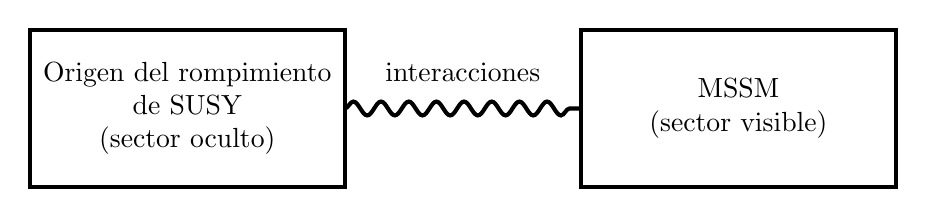
\begin{tikzpicture}

  \draw[line width=1.5] (0,0) rectangle (4,2) node[midway,align=center] (r1) {Origen del rompimiento\\ de SUSY\\ (sector oculto)};
  \draw[line width=1.5] (7,0) rectangle (11,2) node[midway, align=center] (r2) {MSSM\\ (sector visible)} ;

  \draw[line width=1.5,decorate,decoration={snake}] (4,1) -- (7,1) node[midway,above=.2cm] {interacciones};

\end{tikzpicture}

\end{figure}

Existen muchas propuestas de como estas interacciones
mediadores puede ser. Una de estas (e historicamnete la mas popular)
es que estas interacciones son gravitacionales (SUGRA). Mas precisamente
estas asociados con la nueva física, incluyendo a la gravedad, que
aparece cerca de la escala de Planck. En este escenario

Una segunda posibilidad es que estas interacciones mediadores sean
as interacciones de gauge electrodébil y QCD ordinarias. En estos
escenarios donde el rompimiento de supersimetría esta mediado por
campos de gauge (GMSB), los términos soft del MSSM provienen de
diagramas a un loop que involucran algunas partículas mensajeras.

Si tenemos en cuenta a la gravedad, la supersimetría tiene que ser
promovida a una simetría local. Esta teoría supersimétrica local
es llamada \emph{supergravedad}. Esto unifica necesariamente las
simetrías espacio-temporales ordinarias de la Relatividad General
con las transformaciones locales supersimétricas. En esta teoria,
el graviton de spin 2, tiene un supercompa\~nero fermión de spin 3/2
llamado \emph{gravitino}. Mientras la supersimetría no este rota,
el graviton y el gravitino son no masivos con dos estados de helicidad
de spin. Una vez que SUSY es espontáneamente rota, el gravitino adquiere
una masa absorbiendo el goldstino, que se convierte en sus componentes
longitudinales (helicidad $\pm 1/2$). Este mecanismo es llamado \emph{super-Higgs},
y es el análogo al mecanismo de Higgs ordinario de las teorías de gauge,
donde los bosones de gauge $W^\pm$ y $Z^0$ en el {\SM} adquieren
masa absorbiendo los bosones de Nambu-Goldstone asociados con la
invarianza de gauge electrodébil espontáneamente rota. La masa del
gravitino es tradicionalmente llamada $m_{3/2}$, y puede ser estimada
como

\begin{equation}
  m_{3/2} \sim \avg{F} / M_P
\end{equation}

Esto implica distintos valores esperados para la masa del gravitino
dependiendo el modelo de mediadores propuesto. En modelos de mediación
por gravedad, la masa del gravitino es comparable a la masa de las
sparticulas del MSSM, por lo tanto es esperado que sea de al menos
el orden de 100 \gev. Sus interacciones van a ser de intensidad
gravitacional, el gravitino no juega ningún rol en física de
colisiona dores, pero puede ser importante en cosmología.

En contraste, los modelos GMSB predicen un gravitino mucho mas
liviano que las sparticulas del MSSM si $M_\text{mess} \ll M_P$.
En este caso, el gravitino es la LSP, y todas las sparticulas
del MSSM van a decaer eventualmente en un estado final que incluye
el gravitino.








%------
% GMSB
%------
\section{GMSB} %%Modelos de rompimiento de supersimetría mediados por campos de Gauge}

En los modelos de rompimiento de la supersimetría mediado por campos de gauge
(GMSB), las interacciones ordinarias de gauge son los responsables de la
aparición del rompimiento de la supersimetría \emph{soft} en el MSSM.
La idea básica es introducir
nuevos supermultipletes quirales, llamados mensajeros, que se acoplen ...
\note{Referencia: arxiv:9801271}

Estos modelos ofrecen una rica variedad de signaturas en colisionadores\note{0911.4130}.
La caracteristica mas destacable de estos modelos es el gravitino liviano
$m_{3/2} = M_\text{weak}$. Esto asegura que los efectos de mediacion por
campos de gauge domine por sobre la mediacion por gravedad. Esto implica
que la particula mas liviana del MSSM es la NLSP, que siempre decaera
en un gravitino y un companero del SM.
El gravitino siempre va a escapar del detector, dejando una cantidad
significativa de energia faltante. Mientras tanto, el companero del SM va
a tender a ser central y energetico (asumiendo que la NLSP decae promptly),
ya que es en general mucho mas liviano que la NLSP. Dado que en cada evento
SUSY se producen dos NLSPs, es claro que las signaturas en un colisionador
van a estar determinadas por la naturaleza de la NLSP.


In gauge-mediated supersymmetry breaking, gauge forces
transmit the supersymmetry breaking to the MSSM. A typical
structure of such models involves a hidden sector where supersymmetry
is broken, a messenger sector consisting of particles
(messengers) with SU(3)×SU(2)×U(1) quantum numbers, and
the visible sector consisting of the fields of the MSSM [38–40].
The direct coupling of the messengers to the hidden sector generates
a supersymmetry-breaking spectrum in the messenger
sector. Finally, supersymmetry breaking is transmitted to the
MSSM via the virtual exchange of the messengers. In models
of direct gauge mediation, the supersymmetry-breaking sector
includes fields that carry Standard Model quantum numbers, in
which case no separate messenger sector is required [41].

The gravitino mass in models of gauge-mediated supersymmetry
breaking is typically in the eV range (although in some
cases it can be as large as a GeV), which implies that Ge is
the LSP. In particular, the gravitino is a potential dark matter
candidate (for a recent review and guide to the literature, see
Ref. 17). The couplings of the helicity ±1/2 components of Ge
to the particles of the MSSM (which approximate those of
the goldstino, cf. Section I.2.3) are significantly stronger than
gravitational strength and amenable to experimental collider
analyses



\subsection{La LSP: El gravitino}

Como resultado del rompimiento espontaneo de la supersimetria, el espectro fisico
contiene un fermion no masivo de spin 1/2, el goldstino. Cuando la teoria supersimetrica
global esta acoplada a la gravedad y promocionada a una teoria supersimetrica local,
el goldstino provee los modos longitudinales de spin 3/2 del graviton: el gravitino.
Como resultado de este mecanismo de super-Higgs, el gravitino adquiere una masa
que bajo la condicion de la anulacion de la constante cosmologica esta dada por:

\begin{equation}
  m_{3/2} = \frac{F_0}{\sqrt{3}M_P}
\end{equation}
%
donde $M_P = (8\pi G_N)^{-1/2} = 2.4 \times 10^{18} \gev$ es la masa reducida de Planck.
Y $F_0$ es la contribucion total del VEV de rompimiento de SUSY de los campos auxiliares
normalizado de tal forma que la energia de vacio de la teoria supersimetrica global es
$V = F_0^2$...

En los modelos GMSB, el gravitino es la particula supersimetrica mas liviana (LSP) para
cualquier valor relevante de $F$. Si la paridad-R es conservada, todas las particulas
supersimetricas van a seguir cadenas de decaimineto que terminan en gravitinos.

%% Para
%% calcular la tasa de decaimiento
%% La caracteristica mas representativa de los modelos GMSB es el gravitino liviano

\subsection{La NLSP}

\hl{La NLSP puede ser cualquier .... Focus on neutralino NLSP}

La segunda particula supersimétrica mas liviana (NLSP) juega un rol
fundamental en la fenomenología de los modelos GMSB. Asumiendo que se
conserva la paridad-R, todas las particulas supersimétricas van a decaer
rapidamente en una cascada hasta la NLSP, y esta va a decaer en un gravitino
via interacciones 1/F. Por este motivo, la naturaleza de la NLSP
determina las signaturas en los colisionadores y algunas propiedades
cosmologicas del GGM. La NLSP puede ser, dependiendo de la eleccion \note{ref a http://arxiv.org/pdf/hep-ph/9801271v2.pdf}
de los parametros, el neutralino, el stau, y en algunas regiones del
espacio de parametros muy restrictivas, el sneutrino.

En el caso de que sea neutralino, esta tiene, en la mayoria de los
casos, una componente dominante de bino, ya que el cociente $\mu/\M{1}$
es generalemente mayor a 1. %Una excepcion ocurre para N grande y M y lambda
%chico?

Las tazas de decaimiento del {\ninoone} NLSP son:\note{pongo las formulas?}

\begin{align}
  \Gamma (\ninoone \to \gamma \gravino) =
\end{align}

Las particulas, que aunque no son NLSP, tienen un decaimiento dominante en
su companero supersimetrico y el {\gravino} se denominan \emph{co-NLSP}.
Para valores grandes de $\tan \beta$, las dos primeras generaciones de
sleptones decaen como $\susy{\ell}_R \to \ell \tau \stau$ y el stau
es la ``unica'' NLSP. Otra posibilidad es que el {\ninoone}, aunque no sea
la NLSP, esta degenerado en masa con el {\stau}, y su decaimiento dominante
sea a un foton y un goldstino. En este caso {\stau} y {\ninoone} son co-NLSP.

La posibilidad de que el sneutrino sea NLP es muy marginal. Requiere valores
de $N$ tan grandes y valores tan chicos de $\Lambda$ que el descubrimiento de
SUSY deberia darse muy pronto. En este caso el sneutrino decae en un neutrino
y un goldstino.

Todos estos casos corresponden a una fenomenologia completamente diferente en
los experimentos de altas energias.

\subsection{Neutralino NLSP}

En el caso de que la NLSP sea el neutralino, la fenomenología se puede entender
mejor yendo a algunos limites simplificados de los autoestados. De esta forma
los distintos tipos son:

\begin{itemize}
\item bino NLSP
\item wino co-NLSP
\item higgsino NLSP
\end{itemize}

%% We will formulate minimal spectra in this paper which allow for significant strong SUSY production at the early LHC,
%% and populate the many final states   available to general neutralino NLSPs.

%% El espacio de parámetros consiste esencialmente en una escala de producción de color (masa del gluino)
%% y la masa de la NLSP. Todas las demás sparticulas se desacoplan que no son esecnailes en la producción
%% de la signatura de interés. De alguna forma, esto es similar a utilizar ``modelos simplificados'' como
%% se utilizan en muchos estudios fenomenológicos y experimentales. \todo{add references?}

El neutralino NLSP decae a $X + \gravino$, donde $X=\gamma, Z, h$, y los
diferentes autoestados de gauge se caracterizan por tener distintos
BR a las diferentes $X$.

  %% The branching fractions of the bino-like and wino-like neutralino NLSP are shown in the figure.
  %% \includegraphics[width=0.5\textwidth]{br_bino}
  %% \includegraphics[width=0.5\textwidth]{br_wino}

Los binos decaen a fotones con un BR $\sim \cos^2\theta_W$, con una componente menor a Z's, con
BR $\sim \sin^2\theta_W$.
Por otro lado estos BR se intercambian en el caso de que la NLSP sea el wino neutro, que decae
mayormente a Z's.
Si la NLSP es higgsino, este decae en forma dominante a Z o $h$, con branching ratio que depende
en el valor de $\tan\beta$ y del signo de $\mu$. Hay tres casos:

\begin{itemize}
\item El decaimiento del higgsino es dominantemente a Z a bajo $\tan\beta$ y $\mu$ positivo,
\item rico en $h$ a bajo $\tan\beta$ y $\mu$ negativo,
\item y una mezcla de $Z$ y $h$ a moderado y alto $\tan\beta$.
\end{itemize}

Cuando la NLSP es mayormente wino, hay una muy pequena degeneracion entre el wino neutro y el
cargado. Cuando esto pasa, el decaimiento de tres cuerpos al wino neutro comienza
a ser excluido, y el wino cargado prefiere decaer directamente a $W^{\pm}$ y un gravitino.
En otras palabras, el wino neutro y el wino cargado se vuelve co-NLSPs, y los estados finales van
a contener $W$'s, $Z$'s y fotones.

Por otro lado, la degenraci\'on entre los higgsinos cargados y neutros es generalmente mayor, de modo
que solo el neutralino mas livinao decae directamente en gravitino.

El espectro simplificado se muestra en la figura. Básicamente consideramos variar
la masa del gluino (\M{3}) y la masa de la NLSP (\M{1}, \M{2} ó $\mu$ dependiendo
si la NLSP es bino, wino ó higgsino, respectivamente). Todos los demás estados
están desacoplados (sus masas seteadas a 2.5 \tev), ya que no juegan un rol importante
en las signaturas que nos interesan.

\begin{figure}[h]
  \centering
  \includegraphics[width=0.5\textwidth]{figures/figura}
\end{figure}

%% We emphasize that these minimal
%% parameter spaces do correspond to physical models, since the entire GGM parameter space
%% was covered by a perturbative messenger model in [10]

%% Our simplified spectra are characterized by several types of SUSY production, with NLO
%% cross-sections shown in figure 4. For each benchmark, there is colored gluino production, with
%% rate set by the gluino mass. For the wino and higgsino NLSPs, there is also the possibility of
%% direct NLSP production with electroweak cross-sections. While the Tevatron currently has
%% the advantage here because of its much larger dataset, we will see below that the LHC will
%% have sensitivity to electroweak production with & 1 − 5 fb −1

%% \subsection{Bino NLSP}

El decaimiento dominante cunando la NLSP es mayoritariamente bino es a un foton y gravitino.
El principal canal es el de dos fotones ya que la BR es de aproximadamente $(\cos^2\theta_W)^2 \sim 0.6$,
y ademas tiene un bajo fondo del SM.

%% \subsection{Wino co-NLS}

%% \subsection{Z-rich higgsino NLSP}

Higgsinos introduce  an important difference in the topology of the gluino decays. In the bino and wino benchmarks, the gluino decayed 3-body to the neutralino and two jets,
through an off-shell squark. But the higgsino couples predominantly yo heavy flavor, where the mass of the top can squeeze out the 3-body decays. In this regime, the dominant gluino decay is
a one-loop two body decay, $\gluino\to g\susy{H}_{1,2}$.

%% \subsection{Other higgsino types}

The higgsino dominantly decays to Z's at low tanb and positive mu. For larger values of tanb, the higgsino decays to a roughly even mixture of Z's and h's


\section{Producción de partículas supersimétricas} %% en el LHC}

\note{add gluino production.decays diagrams, two-body, three-body}

En los colisionadores hadronicos, las sparticulas pueden ser producidas en pares a partir
de colisiones de partones de \hl{electroweak strength}.

\begin{align}
  &q\bar{q} \quad \to \quad \chinop \chinom, \nino \nino \label{eq:qq_ewk} \\
  &q\bar{q} \quad \to \quad \susy{\ell}^{+}_{i}\susy{\ell}^{-}_{j}, \susy{\nu}_{\ell}\susy{\nu}^{*}_{\ell} \label{qq_ewk2}\\
\end{align}

y reacciones de \hl{QCD strength}:

\begin{align}
  gg \quad &\to \quad \gluino\gluino, \susy{q_i}\susy{q_j}^{*}, \label{eq:gg}\\
  gq \quad &\to \quad \gluino\susy{q_i}, \label{eq:gq} \\
  q\bar{q} \quad &\to \quad \gluino\gluino, \susy{q_i}\susy{q_j}^{*}, \label{eq:qqbar} \\
  qq \quad &\to \quad \susy{q_i}\susy{q_j}, \label{eq:qq} \\
\end{align}

La producciones en \cref{eq:qq_ewk,eq:qq_ewk2}  obtienen contribuciones de los bosones vectoriales
electrodébiles en el canal $s$, mientras que las de \cref{eq:qq_ewk} también tienen contribuciones
del canal $t$ que son menos importantes en la mayoría de los modelos.
Los procesos en \cref{eq:gg,eq:gq,eq:qqbar,eq:qq} tienen contribuciones del intercambio
del correspondiente squark o gluino en el canal $t$, y \cref{eq:gg} y \cref{eq:qqbar}
también tienen contribuciones de gluones en el canal $s$.

\note{Agregar diagramas?}

%% En Tevatron, los procesos de produccion de charginos y neutralinos tienden a tener
%% mayores seccion eficaz, a menos los squarks o el gluino sean muy liviano (menos a 300 \gev,
%% masas que ya se encuentran excluidas por el LHC). En el LHC, la situacion es opuesta, con la
%% produccion de gluinos y squarks dominante por medio de gluon-gluon y gluon-quark fusion.
%% En ambos colisionadores, puede haber produccion asociada de chargino o neutralino junto con
%% un squark y un gluino, pero la mayoria de los modelos predicen que la seccion eficaz


%\part{Experimento}
%% \chapter{El LHC y el detector ATLAS}
\label{cap:detector}

\section{LHC}

El Gran Colisionador de Hadrones (LHC, del inglés \emph{Large Hadron Collider})
\cite{Evans:1129806} es el acelerador de hadrones del Centro Europeo para la
Investigación Nuclear (CERN), ubicado en la frontera entre Francia y Suiza.
Posee una longitud de 27 km y fue construido en el mismo túnel en el que
funcionaba el acelerador $e^{+}e^{-}$ LEP \cite{LEP} (entre 1989 y 2000), a una
profundidad variable entre 50 y 174 m de la superficie.

El complejo de aceleradores del CERN (ver \cref{fig:lhc_complex}) es una
sucesión de aceleradores, en la cual cada acelerador inyecta el haz de protones
en el siguiente, que se encarga de elevar la energía un poco más. El LHC, que es
el último elemento en la cadena, está diseñado para acelerar cada haz de
protones a 7 \tev, alcanzando en las colisiones energías de centro de masa de
14 \tev y una luminosidad de $10^{34}$ cm$^{-2}$s$^{-1}$. Los demás
aceleradores en la cadena poseen además otros experimentos que utilizan los
haces a menores energías.

El número de eventos producidos en un colisionador, como el LHC, está dado
por:

\begin{equation}
  N = L \, \sigma
\end{equation}
%
donde $\sigma$ es la sección eficaz del proceso físico y $L$ es la luminosidad integrada del
acelerador.

La luminosidad instantánea es uno de los parámetros más importantes para
caracterizar el funcionamiento del acelerador, definida como el número de
partículas (protones o iones pesados en el caso del LHC) por unidad de tiempo y unidad de
área, y puede calcularse mediante la relación:

\begin{equation}
  \mathcal{L} = f_\text{rev} n_b \frac{N_1 N_2}{A}
\end{equation}
%
donde $f_\text{rev}$ es la frecuencia de revolución ($\sim 11$ kHz), $n_b$ es el número de
\emph{bunches} (paquetes de protones) por haz, $N_i$ es el número de partículas
en cada \emph{bunch} y $A$ es la sección efectiva del haz, que puede expresarse en
término de los parámetros del acelerador como:

\begin{equation}
  A = \frac{4\pi \epsilon_n \beta^{*}}{\gamma F}
\end{equation}
%
donde $\epsilon_n$ es la emitancia transversal normalizada (la dispersión
transversal media de las partículas del haz en el espacio de coordenadas e
impulsos), $\beta^{*}$ es la función de amplitud en el punto de interacción,
relacionada al poder de focalización de los cuadrupolos), $\gamma$ es el
factor relativista de Lorentz y $F$ es un factor de reducción geométrico, debido
al ángulo de cruce de los haces en el punto de interacción.

\begin{figure}[!p]
  \centering

  \includegraphics[width=0.9\textwidth]{lhc_complex}

  \caption{Complejo de aceleradores del CERN, incluyendo al LHC y a la serie
    de aceleradores utilizados para proveer de protones al LHC. También pueden verse
    los diferentes experimentos ubicados en el acelerador.}
  \label{fig:lhc_complex}

\end{figure}

El diseño del LHC contempla trenes de 2808 paquetes de $\sim 10^{11}$ protones cada uno,
espaciados temporalmente en $\unit[25]{ns}$.
Para acelerar los haces de protones y mantenerlos en sus órbitas circulares el
LHC cuenta con 1232 dipolos magnéticos superconductores que generan un campo
magnético de $\unit[8.4]{T}$ enfriados a $\unit[1.9]{K}$. El sistema de focalización de los haces
consiste de 392 cuadrupolos magnéticos que generan campos magnéticos de $\unit[6.8]{T}$.
Los haces circulan en direcciones opuestas en cavidades de ultra alto vacío
a presión de $\unit[10^{-10}]{torr}$.

Durante el año 2012, las colisiones se realizaron a $4\TeV$ por haz ($\sqrt{s} = 8 \TeV$)
y con una luminosidad que fue incrementándose hasta alcanzar los
$\unit[2 \cdot 10^{32}]{cm^{-2}s^{-1}}$ en Octubre. Durante los a\~nos 2013 y 2014
el LHC no estuvo en funcionamiento, y se utilizó este tiempo para prepararlo para
la nueva etapa que comenzó en el a\~no 2015, en el cual se alcanzó una energía de $\sqrt{s} = 13 \tev$,
una energía que nunca antes había sido alcanzada y cercana a la de su diseño
original (14 \tev).



\section{El detector ATLAS}

ATLAS (\emph{A Torodial LHC AparatuS}) es un detector de partículas
multipropósito del LHC, diseñado y construido para estudiar las colisiones
protón-protón (y de iones pesados) y un gran espectro de procesos físicos en la
escala de energía del \tev.

\begin{figure}[!p]
  \centering

  \includegraphics[width=\textwidth]{atlas}
  \caption{Esquema general del detector de ATLAS. Las dimensiones del detector
    son $\unit[25]{m}$ de altura y $\unit[44]{m}$ de largo. El peso promedio es
    de aproximadamente 7000 toneladas.}
  \label{fig:atlas}

\end{figure}

El esquema general del detector se muestra en la \cref{fig:atlas}, donde se
señalan los componentes principales. ATLAS está diseñado en capas de
subdetectores que cumplen diferentes roles en la identificación de las
partículas producidas durante las colisiones (ver \cref{fig:how_atlas_works}).
Desde el punto de la colisión
hacia afuera ATLAS se compone de un detector interno de trazas (ID) compuesto de
un detector de píxeles, un detector de bandas de silicio (SCT) y un detector de
radiación de transición (TRT).
Por sobre el detector interno se encuentra un
solenoide superconductor que genera un campo magnético de $\sim \unit[2]{T}$, a fin
de curvar la trayectoria de las partículas cargadas.
A continuación están ubicados los calorímetros. En primer lugar el calorímetro
electromagnético para medir la energía cinética de electrones y fotones, y
posteriormente el calorímetro hadrónico para medir la energía de los jets.
En la capa más externa se encuentra el espectrómetro de muones que le da a ATLAS
el tamaño total de aproximadamente $\unit[45]{m}$ de largo y más de
$\unit[25]{m}$ de alto. Intercalado con éste se encuentra el sistema de toroides
que genera el campo magnético de $\sim \unit[4]{T}$ para curvar la trayectoria de
los muones hacia el final de su pasaje por el detector ATLAS.

El detector ATLAS se divide geométricamente en dos regiones, la parte central
denominada \emph{barrel}, y la región de las tapas llamadas \emph{end-caps}.
En cada una de estas regiones la ubicación de los
subdetectores es distinta. En la región \emph{barrel}, los subdetectores están
ubicadas como cilindros concéntricos, mientras que en la región \emph{end-cap}
están ubicados como discos consecutivos perpendiculares a la dirección del haz.


\begin{figure}[!p]
  \centering

  \includegraphics[width=0.8\textwidth]{how_atlas_works_invert}

  \caption{Esquema del corte transversal del detector de ATLAS, ilustrando los distintos
  subdetectores y el pasaje de las distintas partículas.}
  \label{fig:how_atlas_works}

\end{figure}


\subsection{Sistema de coordenadas}

%% El sistema de coordenadas de ATLAS corresponde a un sistema cartesiano, cuyo
%% origen coincide con el punto de interacción nominal. El eje $z$ es escogido,
%% naturalmente dazda la concepción cilíndrica del detector, a lo largo del eje del
%% haz, en sentido antihorario.

El sistema de coordenadas y la nomenclatura utilizada para describir el detector
ATLAS y las trayectorias de las partículas que emergen de las colisiones son
resumidas en esta sección, ya que se utilizarán a lo largo de la tesis. Se
define como origen de coordenadas al punto de interacción nominal, mientras que
la dirección del haz define el eje $z$ y el plano $x-y$ es el transversal a la
dirección del haz. El eje $x$ se define desde el punto de interacción, apuntando
al centro del anillo del LHC, y el eje $y$ se define apuntando hacia arriba.

%% El plano transversal $x-y$ es definido con valores positivos de $x$ e $y$
%% desde el origen en dirección hacia el centro del anillo del LHC y hacia la
%% superficie, respectivamente.
Para describir la posición de los distintos
subdetectores y la trayectoria de las partículas dentro de ATLAS se utilizan
frecuentemente sistemas de coordenadas cilíndricas o polares. El radio $R$ se
define como la distancia perpendicular al eje del haz. El ángulo azimutal $\phi
$ es medido alrededor del eje del haz, mientras que el ángulo polar $\theta$
es el ángulo respecto al eje del haz.

Una cantidad muy importante utilizada en física de altas energías es la
llamada rapidez:

\begin{equation}
  y = \frac{1}{2} \ln \left( \frac{E+p_z}{E-p_z} \right)
\end{equation}
%
donde $E$ es la energía total de la partícula y $p_z$ es la componente
longitudinal de su impulso. En el límite de altas energías esta cantidad se
aproxima (en forma exacta para objetos no masivos) por la llamada
\emph{pseudorapidez}, $\eta$, relacionada con el ángulo polar $\theta$ como:

\begin{equation}
  \eta = - \ln \tan \left( \frac{\theta}{2} \right)
\end{equation}

La razón detrás de esta transformación de coordenadas es el hecho que la
multiplicidad de partículas producidas es aproximadamente constante como función
de $\eta$, y que la diferencia de pseudo-rapidez entre dos partículas es
invariante frente a transformaciones (\emph{boosts}) de Lorentz a lo largo de la
dirección del haz. En el caso de colisiones hadrónicas, la fracción del impulso
del protón adquirida por cada uno de las partones interactuantes es desconocida.
Parte de este impulso es transferido en la interacción dura, mientras cierta
fracción remanente escapa el detector a lo largo del haz. Así, no es posible
reconstruir el movimiento longitudinal del centro de masa en la interacción, y
aplicar leyes de conservación sobre la cinemática de cada evento. Sin embargo,
dado que los protones inciden a lo largo de la dirección del haz, el impulso
total transverso es conservado durante la colisión. Por esta razón, solo las
componentes transversales son utilizadas en la descripción de la cinemática del
evento, por ejemplo $\pt (= p \sin \theta)$. En términos de
la pseudo-rapidez, se define la energía transversa ($\et = E \sin \theta$) de una partícula como:


\begin{equation}
  \et = \frac{E}{\cosh \eta}
\end{equation}
%
donde $E$ es su energía total.


\section{Los subdetectores de ATLAS}

%% A continuación se describen brevemente cada uno de los subdetectores,
%% particularmente aquellos subsistemas utilizados para la identificación de
%% electrones y fotones, pertinentes al análisis presentado en esta Tesis.

\subsection{El detector interno}

El esquema del detector interno se muestra en la \cref{fig:detector_interno} y a
continuación se describen los distintos componentes del mismo. Este sistema
combina detectores de muy alta resolución para distancias cortas al punto de
interacción con detectores continuos de trazas a distancias más lejanas. El
detector interno está contenido dentro del solenoide que provee un campo
magnético nominal de $\unit[2]{T}$.

\begin{figure}[!p]
  \centering

  \includegraphics[width=0.6\textwidth]{detector_interno}
  \caption{Esquema del detector interno mostrando la traza de una partícula
    cargada de $\pt = 10\gev$ atravesándolo. La trayectoria atraviesa el
    tubo del haz de berilio, las tres capas del detector de píxeles de silicio (Pixels),
    las cuatro capas dobles de sensores semiconductores (SCT), y
    aproximadamente 36 tubos contenidos en los módulos del detector por radiación
  de transición (TRT).}\label{fig:detector_interno}

\end{figure}

\subsubsection{Detector de Píxeles}

Más cerca del punto de interacción se encuentra el detector de píxeles
\cite{Wermes:381263}, cuyo objetivo principal consiste en la medición de la
posición de trazas de partículas cargadas con la más alta precisión posible y es
de vital importancia para la reconstrucción de los vértices primarios y
secundarios. El principio de detección para partículas cargadas es la medida de
la deposición de la carga inducida en una capa de silicio por ionización.
Se compone de tres capas en la región \emph{barrel} (a 4, 10 y 13 cm del tubo
del haz) y tres discos en cada \emph{end-cap}.
La primer capa, conocida como capa-$B$, está ubicada a $\unit[50.5]{mm}$ del
punto de interacción, permitiendo obtener una resolución óptima del parámetro de impacto.
El sistema contiene en total 80 millones de sensores electrónicos, capaces de
resolver la posición de las partículas mejor que $\unit[14]{\mu m}$.


\subsubsection{Detector Semiconductor de Trazas (SCT)}

Por fuera del detector de píxeles se encuentra el detector semiconductor de
trazas (SCT) que consta de ocho capas de detectores de micro bandas de silicio
que provee puntos de alta precisión en las coordenadas (R$\phi$,z).
La
resolución espacial es de 16 $\mu$m en R$\phi$ y de 580 $\mu$m en z y tiene 6.2
millones de canales. Las trazas pueden distinguirse si están separadas más de
$\sim$200 $ \mu$m. El SCT cubre el rango de pseudorapidez de $|\eta|<$2.5.


\subsubsection{Detector de Radiación de Transición (TRT)}

La parte más externa del detector de trazas es el detector de radiación de
transición (TRT). Este detector está basado en el uso de tubos detectores que
pueden operar a alta frecuencia de eventos gracias a su pequeño diámetro ($\unit[4]{mm}$) y
el aislamiento de sus hilos centrales en volúmenes de gas individuales.

El TRT además de detectar el pasaje de partículas cargadas, detecta la radiación
de transición que permite distinguir entre partículas cargadas pesadas y
livianas. La separación entre señales de trazas y de radiación por transición se
hace analizando tubo por tubo impactos de alto umbral e impactos de baja señal.
El largo de los tubos varía según la zona del detector, llegando hasta los 144
cm en la zona central. El \emph{barrel} contiene 50000 tubos y las
\emph{end-caps} contienen 320000 tubos orientados radialmente. El número total
de canales es de 420000 y la resolución espacial es de $\unit[0.17]{mm}$.


\subsection{Calorímetros}

Un esquema de los calorímetros de ATLAS puede verse en la \cref{fig:calorimetros}.
Consta de un calorímetro electromagnético cubriendo la región de pseudorapidez
$|\eta| < 3.2$, un calorímetro hadrónico en la sección \emph{barrel} cubriendo
la región $|\eta| < 3.2$, calorímetros hadrónicos en las \emph{end-cap} cubriendo
la región $1.5 < |\eta| < 3.2$, y calorímetros \emph{forward} cubriendo $3.1 < |\eta| < 4.9$.


\subsubsection{Calorímetro electromagnético}

\begin{figure}[!p]
  \centering

  \includegraphics[width=0.9\textwidth]{calorimetros}

  \caption{Sistema de calorímetros del detector de ATLAS}
  \label{fig:calorimetros}

\end{figure}

El calorímetro electromagnético \cite{caloemTDR} se divide en una parte central
($|\eta|<$1.475) y los \emph{end-caps} (1.375$<|\eta|<$3.2). La parte central
está compuesta por dos mitades, separadas por una
distancia pequeña ($\unit[6]{mm}$) a $z = 0$. Las tapas del calorímetro están divididas en
dos ruedas coaxiales, una rueda externa cubriendo la región 1.375$<|\eta|<$2.5 y
una parte interna que cubre la región 2.5$<|\eta|<$3.2.

El calorímetro electromagnético es un detector de muestreo de argón líquido
(LAr) con electrodos de \emph{kapton} en forma de acordeón y planchas absorbentes de
plomo. El espesor total del calorímetro electromagnético es $>24 X_0$ en el
barril y $>26 X_0$ en las tapas, donde $X_0$ es la longitud de radiación.

En la región dedicada a los estudios de física de precisión ($|\eta|<$2.5) el
calorímetro electromagnético está segmentado en tres secciones longitudinales.

La sección de las bandas (\emph{strips}) que tiene un espesor constante de
$\sim 6 X_0$ en función de $\eta$, está equipado con bandas finas de $\unit[4]{mm}$ de
largo en la dirección $\eta$. Esta sección actúa como un detector de pre-cascada
aumentando la capacidad de identificación de partículas,
(como por ejemplo la distinción entre $\gamma$ y $\pi_0$ o entre electrón y
$\pi^\pm$) y dando una precisa medición de la posición en $\eta$.
La sección del medio está segmentada transversalmente en torres cuadradas de
$\Delta \phi \times \Delta \eta = 0.025 \times 0.025$ ($4 \times \unit[4]{cm^2}$ en
$\eta=0$). El espesor total del detector hasta el final de la sección del medio
es $\sim 24 X_0$.
La sección más externa tiene una granularidad de
$\Delta\phi\times\Delta\eta = 0.025 \times 0.05$ y su espesor varía entre 2 y 12
$X_0$.


\subsubsection{Calorímetro hadrónico}

El calorímetro hadrónico de ATLAS \cite{calohadTDR} cubre el rango $|\eta|<$4.9
usando diferentes materiales.
La parte del \emph{barrel} de este sistema consiste en un calorímetro de muestreo que
utiliza acero como absorbente y tejas centelladoras como material activo. Las
tejas están ubicadas radialmente y apiladas en profundidad.

La estructura es periódica en $z$. Las tejas tienen un espesor de $\unit[3]{mm}$ y el
espesor de las placas de acero en un período es de $\unit[14]{mm}$.
El calorímetro de tejas se extiende radialmente desde un radio interno de $\unit[2.28]{m}$
hasta un radio externo de $\unit[4.25]{m}$.

En la región de \emph{end-caps}, el calorímetro hadrónico se compone de dos ruedas de
$\unit[2.3]{m}$ de radio, perpendiculares al tubo del haz, hechas con placas de cobre y
tungsteno como material absorbente y argón líquido como material activo. Estos
detectores extienden la aceptancia del calorímetro de ATLAS hasta prácticamente
cubrir el ángulo sólido del punto de colisión.


\subsection{Espectrómetro de muones}
\label{sec:espectrometro_muones}

Los muones de alto {\pt} generados en el punto de interacción tienen un altísimo
poder de penetración y son poco interactuantes. Por ello el espectrómetro de
muones \cite{muonTDR} se encuentra situado en la parte más exterior del detector
ATLAS, alrededor del sistema de imanes de toroides, y está diseñado para obtener
mediciones de alta precisión de posición e impulso de muones de alto \pt.
Este es el subdetector más grande y el que le da a ATLAS su tamaño.

%% \begin{figure}[!htb]
%%   \centering
%%   \includegraphics[width=0.7\textwidth]{figures/}
%%   \caption{Espectrómetro de muones del detector de ATLAS}\label{fig:especmuones}
%% \end{figure}

%% La \cref{fig:especmuones} muestra un esquema del espectrómetro de muones
%% de ATLAS.

La región del barril está compuesta por tres capas concéntricas de cámaras de
\emph{trigger} y de cámaras de precisión posicionadas a 5m, 7.5m y 10m del tubo del
LHC, cubriendo la región $|\eta|<1$. Las regiones de las tapas están compuestas
por cuatro capas de cámaras de \emph{trigger} y cámaras de precisión a $|z|$= 7.4m,
10.8m, 14m y 21.5m cubriendo el rango de 1.0$<|\eta|<$2.7. Hay una pequeña
brecha en $|z|=0$ que permite el acceso de los servicios al ID.

El espectrómetro de muones es el subdetector más grande de ATLAS, construido
dentro y alrededor de los imanes toroidales. Los muones son altamente penetrantes
y son las únicas partículas (excepto las invisibles que no interactúan) que llegan
al sistema de muones. Los muones pierden parte de su energía mientras penetran
las capas internas de ATLAS antes de llegar al espectrómetro de muones. La pérdida
de energía tiene que ser tenida en cuenta utilizando los depósitos de energía
en los calorímetros.

%% The muon system is exposed to challenging background conditions. Final state
%% particles undergoing secondary interactions in the detector, shielding or surround-
%% ing machine material, result in a large number of particles, mainly photons and
%% neutrons with energy of order ∼ 1 MeV, penetrating the muon system. The muon
%% spectrometer is designed to cope with these high rates of particle flux. Cosmic ray
%% event data was used to measure the muon reconstruction efficiency and the momen-
%% tum resolution of the muon spectrometer [59]. For muons with transverse momenta
%% of ∼ 100 GeV the momentum resolution is at its best, with an expected fractional
%% resolution of ∼ 2 %. At p T ∼ 1 TeV this resolution decreases to ∼ 10 %, and below
%% 100 GeV the resolution also drops off as an increasing fraction of the muon energy
%% is lost traversing the detector material downstream.

%%El sistema de muones incluye
%% The muon system includes a separate trigger designed to identify events contain-
%% ing highly energetic muons, which are interesting for many new physics searches.
%% The muon trigger has coverage up to |η| < 2.4, with the full range of the muon
%% system being |η| < 2.7. Three concentric cylinders surrounding the calorimeters
%% at radii of 5 m, 7.5 m and 10 m comprise the muon system in the barrel. Wheels
%% are placed at distances of approximately 7.4 m, 10.8 m, 14 m and 21.5 m from the
%% interaction point, constituting the muon system in the end-caps. A total of four
%% different technologies are incorporated into the muon system to fulfil the triggering
%% and precision physics requirements. The Monitored Drift Tubes (MDTs) and Cath-
%% ode Strip Chambers (CSCs) provide precision energy measurements and tracking,
%% with the Resistive Plate Chambers (RPCs) and Thin Gap Chambers (TGCs) be-
%% ing responsible for triggering. A particular challenge for the muon trigger system
%% is the ability to maintain a stable p T resolution for the full |η| < 2.4, since the
%% momentum, p, of a muon of a given p T increases as a function of η. This demands
%% increased granularity in the more forward regions of the muon spectrometer so as to
%% ensure a momentum resolution consistent with the barrel. To achieve this different
%% technologies are used in the barrel and end-cap regions of the muon system.
%% The MDTs are gas filled (Ar, CO 2 ) aluminium tubes of diameter ∼ 30 mm with
%% tungsten wires immersed within. When a muon traverses these tubes the gas is
%% ionised and the resulting electrons collect on the tungsten. The MDTs are found in
%% both the barrel and the end-caps, and provide precision position and momentum
%% measurements over the full |η| < 2.7 range of the muon system. A typical MDT
%% chamber consists of two multi-layers of drift tubes, which are separated by spacer
%% bars made of aluminium. Each of these multi-layers contains four layers of tubes
%% in the barrel, or three in the outer regions of the muon system. This means that a
%% muon penetrating the MDTs will on average pass through 20 individual tubes.
%% The safe operational counting rate per unit area for the MDTs is exceeded in
%% the forward regions of the muon system. Cathode strip chambers, with a quicker
%% response time and double the resolution, are used in this region. The CSCs cover the
%% range 2.0 < |η| < 2.7 and are used in the innermost part of the muon system in the
%% end-caps. They are multi-wire proportional chambers containing multiple closely
%% spaced anode wires surrounded by gas (Ar, CO 2 , CF 4 ), with cathode strips running
%% perpendicular to the wires. This orthogonal layout allows the charge distribution
%% to be measured in both directions normal to the beam axis. The CSC system itself
%% is segmented in φ, resulting in eight chambers in each of the two disks. With four
%% CSC layers in each chamber, the average number of measurements per track is
%% considerably less than in the MDTs.
%% The RPCs make up the barrel part (|η| < 1.05) of the dedicated trigger system.
%% Two resistive plates are separated by 2 mm of gas (C 2 H 2 F 4 , Iso-C 4 H 10 , SF 6 ), which
%% may be ionised by a muon passing through, causing a cascade of electrons towards
%% the anode. These chambers are made simpler in construction due to the absence
%% of any wires within, and this feature also makes them less sensitive to any small
%% deviations in positioning (e.g. wire sag). There are three cylindrical trigger layers
%% in the barrel, and each layer contains two RPCs. As such, a muon in the barrel will
%% deliver six hits in the RPCs. The RPCs are able to provide adequate triggering for
%% the barrel region.
%% In addition to the increased demands on granularity, the forward region suffers
%% from radiation levels up to 10 times those in central regions. This further compli-
%% cates the already challenging environment in the end-caps. The TGCs are used to
%% trigger on muon tracks in the end-caps (1.05 < |η| < 2.4). They are multi-wire
%% proportional chambers working similarly to the CSCs, but in this case in order to
%% satisfy the higher granularity requirements the gap between the wire and cathode
%% is smaller than the wire-wire spacing. They exist in two concentric rings, one inner
%% ring containing two TGC layers and one outer ring containing seven. These layers
%% are segmented radially, are tailored to provide excellent time resolution and are able
%% to cope with high particle flux rates. Both the TGCs and RPCs are designed to
%% deliver signals over a time spread of less than 25 ns. This way the bunch crossing
%% responsible for the muon triggering the chamber can be identified with an efficiency
%% of > 99 %.


%---------
% Trigger
%---------
\section{El sistema de \emph{trigger}}

La parte central del sistema de adquisición de datos de ATLAS es el
<<\emph{trigger}>>. El sistema de \emph{trigger} puede ser pensado como un filtro que
selecciona, del gran número de colisiones que tienen lugar en el experimento,
los eventos que serán almacenadas para su posterior procesamiento y análisis.

El LHC esta diseñado para proveer colisiones $pp$ de $\mathcal{O}(1)$ GHz,
considerando una frecuencia de cruce de haces de $\unit[40]{MHz}$ y $\sim$ 23
interacciones por cruce. Dado que la mayoría de los eventos no son de interés
para los análisis de física, y también debido a las limitaciones de
almacenamiento y de poder de cómputo, el flujo de datos incidente debe ser
reducido al máximo permitido para su almacenamiento permanente ($\sim 400$ Hz)
\cite{Aad:2012xs}.
Esta reducción se logra mediante una rápida y eficiente preselección de eventos,
conocida como \emph{trigger}.

Esencialmente, el sistema de \emph{trigger} de ATLAS \cite{atlas} consiste en
una selección de eventos basada en tres niveles: Nivel 1 (L1), Nivel 2 (L2) y
Filtro de eventos (EF), donde los dos últimos conforman el \emph{High Level
  Trigger} (HLT). Cada nivel permite analizar los eventos con mayor detalle,
aumentando la precisión de los criterios de selección y la complejidad de los
algoritmos utilizados. El sistema de adquisición de datos transfiere y
almacena los datos seleccionados por el \emph{trigger}.

El L1 se encarga de la selección inicial, reduciendo la frecuencia de eventos
que pasan al siguiente nivel a $\sim 75$ kHz. Debido al tamaño limitado de las
memorias temporales donde se guardan los datos de cada subdetector y al
considerable tiempo de vuelo de las partículas hasta el espectrómetro de muones,
la decisión debe tomarse en una escala de tiempo muy limitada ($\unit[2.5]{\mu s}$).
El L1 está basado en hardware y selecciona objetos de alto {\pt}
construidos a partir de la información de varios subdetectores. Los muones son
identificados en las cámaras de \empg{trigger} descriptas en la
\cref{sec:espectrometro_muones}, mientras que la información de los
calorímetros, con una resolución reducida, se utiliza para identificar
candidatos a electrones, fotones, jets y taus decayendo hadrónicamente. La
posición de cada objeto encontrado define una <<región de interés>> (RoI) en
un evento potencialmente interesante, que se extiende como un cono desde el
punto de interacción a lo largo del detector.

En el calorímetro, el L1 se basa en las señales analógicas obtenidas en cada
torre del \emph{trigger}, es decir en la suma de celdas en una ventana $\Delta \eta
\times \Delta \phi = 0.1 \times 0.1$, definida separadamente para el calorímetro
electromagnético y hadrónico. La aceptancia geométrica del L1 está ligada al
diseño del detector, donde las medidas de precisión en los calorímetros y la
cobertura del detector interno están limitadas a la región $\abseta < 2.5$. El
\emph{trigger} de fotones, electrones, muones y taus debe asegurar la cobertura en esta
región. En el caso del \emph{trigger} de jets, las torres del \emph{trigger} se
extienden hasta $\abseta < 3.2$, mientras que para el cálculo de la energía
transversa total (faltante) se utiliza todo el sistema calorimétrico (es decir,
$\abseta < 4.9$). Los resultados de los subsistemas del \emph{trigger} son procesados
en el \emph{Central Trigger Processor}, en donde se aplica una serie de
selecciones definidas como una combinación de criterios individuales, que pueden
ser ajustados según la luminosidad y los requerimientos físicos particulares de
cada toma de datos. Las distintas configuraciones (\emph{items}) están
disponibles en el L1, donde se programa el tipo de RoI (EM, TAU, JET, etc.) y
los umbrales de energía total y de aislamiento requeridos en cada caso. Por
ejemplo, el item L1EM14 acepta eventos donde al menos un (dos) \emph{cluster(s)} en el
calorímetro electromagnético posee(n) $\et \geq 14 \GeV$.

El segundo nivel del \emph{trigger} (L2) se centra únicamente en las RoIs donde el L1
encontró actividad, combinando información de todos los subdetectores dentro de
cada una ($\sim 2$ \% de la cobertura total del detector). El L2 consiste de una
serie de algoritmos de reconstrucción y selección especializados, dise\~nados
para reducir la frecuencia de eventos hasta aproximadamente 1 kHz. Estos
algoritmos están implementados en \emph{clusters} de procesamiento dedicados
que analizan cada evento dentro de un tiempo de latencia medio de $\sim
\unit[40]{ms}$. El menor flujo de información en este nivel del \emph{trigger} permite
calcular las variables calorimétricas con mayor precisión y hacer uso de la
información de las trazas reconstruidas, haciendo posible la distinción entre
fotones y electrones, y el rechazo de fondo proveniente en su mayoría de jets.
En general, si bien la selección se basa en las mismas variables que la
identificación \emph{offline} descripta en la \cref{sec:obj_photons} (sobre las características de
las lluvias electromagnéticas), los valores de corte en cada variable son
relajados (o a lo sumo igualados) respecto a la selección \emph{offline}, para evitar
el rechazo prematuro de candidatos que satisfacen los criterios de identificación
durante el análisis final. La última etapa de la selección del \emph{trigger} se lleva
a cabo en el EF, que reduce la frecuencia de eventos a $\sim \unit[400]{Hz}$.
En este nivel se tiene acceso a toda
la información del evento en los distintos subdetectores de ATLAS, con la máxima
granularidad e incluyendo detalles sobre la calibración de energía de los
calorímetros, la alineación de los subdetectores y el mapa de campo magnético. El
tiempo de latencia relativamente largo disponible para tomar la decisión final
sobre el evento ($\avg{t} \sim \unit[4]{s}$) permite la reconstrucción completa
del mismo, y el refinamiento de las variables y criterios de selección al nivel
de aquellos implementados en el análisis \emph{offline}. Los eventos aceptados por el
EF son finalmente grabados a disco y distribuidos, accesibles \emph{offline} para todos
los análisis subsecuentes.

Al igual que en el L1, en cada nivel del HLT se configuran ciertos
criterios según el tipo y multiplicidad de la partícula que se busca en el
evento, y el conjunto de cortes de identificación aplicados. La nomenclatura
adoptada como convención en el \emph{trigger} de ATLAS tiene la forma general
\texttt{L\_ipX\_Y}, donde \texttt{L} es el nivel del \emph{trigger} (L2,EF), \texttt{i}
la multiplicidad, \texttt{p} la partícula de interés (por ejemplo
\texttt{g} = fotón, \texttt{e} = electrón), \texttt{X} el {\pt} mínimo requerido e
\texttt{Y} el tipo de identificación aplicada (\emph{loose}, \emph{tight}, etc.). Los
distintos criterios del L2/EF y su item asociado en el L1 definen en conjunto
una de las <<cadenas>> del \empg{trigger}, que toman el nombre de la signatura del
HLT (es decir, \texttt{ipX\_Y} según la convención anterior) y conforman el <<menú>> final
del \emph{trigger}.

Para cada item del \emph{trigger} se puede asignar además
un factor de escala o \emph{prescale} (PS), que define la frecuencia con la que un dado
item es evaluado por el \emph{trigger} (es decir solo en uno de cada PS eventos).
Se habla de una cadena de \emph{trigger} \emph{unprescaled} si su factor de escala es
$\text{PS} = 1$ en cada nivel, es decir, es evaluada en todos los eventos. La asignación de estos
factores se hace incluso dinámicamente durante una toma de datos, para tener en
cuenta el descenso de la luminosidad instantánea con el tiempo y mantener la
tasa de procesamiento aproximadamente constante.



\section{Modelo computacional y distribución de datos}

El modelo computacional de ATLAS está diseñado para permitir a todos los
miembros de la colaboración un acceso ágil, directo y distribuido a la gran
cantidad de datos recolectados por el detector ($\sim \text{PB}/\text{a\~no}$),
así como a las diversas simulaciones MC. El modelo se basa en la tecnología
GRID, compartiendo el poder de procesamiento y la capacidad de almacenamiento
disponibles en distintos centros de cómputo asociados alrededor del mundo.

El software de ATLAS se desarrolla dentro un entorno C++ común llamado
\textsc{Athena} \cite{CompuTDR,Lenzi:1214931,Calafiura:865624}, basado en el
proyecto GAUDI \cite{Gaudi}. Todo el procesamiento de los datos en ATLAS se
realiza dentro de este entorno, incluyendo la implementación y configuración del
HLT, la simulación de la respuesta del detector, la generación de las muestras
MC de los distintos procesos físicos, y la reconstrucción y análisis de los
datos. Los eventos aceptados por el \emph{trigger} deben ser procesados para reducir su
tamaño y ser utilizados para los análisis \emph{offline}. A la salida del HLT, los
eventos son almacenados como RDOs (\emph{Raw Data Objects}). Luego de aplicar
los algoritmos de reconstrucción y calibración, las colecciones de los distintos
objetos físicos obtenidas (fotones, electrones, etc.) son almacenadas en formato
ESD (\emph{Event Summary Data}) y AOD (\emph{Analysis Data Object}), una versión
reducida del primero ($\sim 100$ kB/evento). A partir de las ESD/AOD, se ha
definido un formato de datos significativamente más pequeño (10-15 kB/evento)
conocido como D3PD (\emph{Derived Physics Data}), sobre el que se realiza el
análisis final. Las \emph{D3PD} son ntuplas almacenadas en un formato de archivo
accesibles vía el entorno de análisis de datos ROOT \cite{Brun199781}, que
contienen un conjunto de variables para diferentes objetos físicos, según las
necesidades de cada grupo de análisis dentro de ATLAS. Para el análisis de esta
tesis, se utilizaron las D3PD definidas y producidas en forma centralizada por
el grupo de SUSY. La misma cadena de reconstrucción y distribución se aplica a
las simulaciones Monte Carlo, a fin de conservar un modelo de análisis único y
garantizar la consistencia en la comparación de estas con los datos
experimentales.



\section{Datos de colisiones $pp$ a $\sqrt{s} = 8$ \tev}

Durante la operación del detector ATLAS, cada toma de datos (\emph{Run}) durante
un haz estable provisto por el LHC, es dividida en bloques de luminosidad
(\emph{LB}) de aproximadamente dos minutos, dentro de los cuales la luminosidad
instantánea es prácticamente constante, y en el que se espera que las
condiciones del haz sean estables. Producto de la complejidad del experimento y
de las demandantes condiciones de funcionamiento del LHC, se pueden observar
ocasionalmente ciertas ineficiencias en los diversos subdetectores y/o en la
cadena de procesamiento de los datos recolectados. Durante cada \emph{Run} los
distintos subcomponentes del detector son monitoreados y cada problema es
registrado, incluyendo que componentes están inactivos, o si hay problemas en
la infraestructura o en el haz.

Para asegurar la calidad de los datos a ser considerados en los análisis físicos
de ATLAS, los grupos responsables de cada subdetector definen un conjunto de
criterios de calidad \cite{GRL}, con los cuales se construyen listas, llamadas
GRL (\emph{Good Runs List}), de las \emph{Runs} y los rangos de LB dentro de ellas que
son apropiados para cada tipo de análisis. Se producen de forma centralizada
para brindar listas oficiales comunes para los distintos grupos dentro de ATLAS
y son distribuidas en un formato \textsc{XML} para luego ser utilizadas durante
el análisis final. Cada análisis elige que GRL utiliza dependiendo de su
tolerancia a las fallas de los subdetectores.

El presente análisis utiliza el conjunto de eventos recolectados de las colisiones
$pp$ a una energía de centro de masa $\sqrt{s} = 8\tev$ con el detector ATLAS
durante el a\~no 2012. Estos eventos recolectados corresponden a una luminosidad
total integrada de 21.7 \ifb. Dado que en el análisis se utilizan fotones, electrones,
muones, jets y energía faltante, es imprescindible que todos los subsistemas
del detector ATLAS hayan operado en condiciones normales durante la toma
de datos. Este requerimiento adicional resulta en una reducción de los datos de
$\sim 6\%$, dejando una luminosidad total de $\int L\, dt = 20.3 \pm 0.6\, (2.8
\%) \, \ifb$\cite{lumi2012} para análisis físicos.

Otro concepto importante de la toma de datos en ATLAS es el \emph{pile-up}, el
cual ocurre cuando las partículas producidas en más de una colisión
partón-partón llegan al detector al mismo tiempo, o más generalmente que sus
señales se superponen de una forma que no puede ser separadas. Cuando los
\emph{bunches} de protones colisionan, la probabilidad de una interacción es
proporcional a la densidad de partículas, o mejor, al flujo de partículas, el
cual se expresa con la luminosidad instantánea. El número de colisiones de
partículas real que tienen lugar cuando dos \emph{bunches} se cruzan es una
variable aleatoria que sigue una distribución de Poisson. Para bajas
luminosidades, en la mayoría de los cruces de haces, no ocurren colisiones, pero para
luminosidades instantáneas altas, en la mayoría de los cruces se producen muchas
colisiones de partículas al mismo tiempo. Dependiendo del subdetector y el tipo
de medición, puede o no ser posible distinguir entre las partículas provenientes
de diferentes interacciones simultáneas. Esto es llamado \emph{pile-up in-time}.
En cambio, el \emph{pile-up out-of-time} incluye los efectos que se originan
cuando el tiempo que el detector necesita para volver a su estado de espera es
mayor al tiempo entre cruces de \emph{bunches}. Una medida cuantitativa del
\emph{pile-up} y la actividad del evento, es el valor medio de interacciones
inelásticas $pp$ por cruce de \emph{bunches}, $\avg{\mu}$.

Durante el período de toma de datos del 2012, el pico de luminosidad instantánea
aumentó desde $\unit[2.74 \cdot 10^{30}]{cm^{-2} s^{-1}}$ hasta
$\unit[7.61 \cdot 10^{33}]{cm^{-2} s^{-1}}$, y el número medio de interacciones por cruce
de haz varió entre 5.9 y 36.53. La distribución de la luminosidad acumulada
durante la toma de datos y del número de interacciones por colisión pude verse en
la \cref{fig:lumi}.

\begin{figure}[!p]
  \centering

  \includegraphics[width=0.49\textwidth]{intlumivstime2012DQ}
  \includegraphics[width=0.49\textwidth]{mu_2012-dec}

  \caption{Izquierda: Luminosidad acumulada como función del tiempo, entregada por el LHC (verde),
    guardada por ATLAS (amarillo), y que pasa los criterios de calidad (azul),
    durante el funcionamiento del LHC con haces estables en colisiones $pp$ a $\sqrt{s}=8\tev$ durante el a\~no 2012\cite{lumiplots}.
    Derecha: Distribución del valor medio del número de interacciones por cruce
    de haz ($\mu$) durante la toma de datos en el a\~no 2012 pesado con la luminosidad.
    La luminosidad integrada y el valor medio de $\mu$ están detallados en la figura.
  }
  \label{fig:lumi}

\end{figure}

%% \chapter{Reconstrucción de objetos físicos} %\section{Selección de objetos}
\label{sec:obj_selection}

%% In this section a description of the reconstruction and calibration is given for
%% the main physics objects this analysis has to deal with (photons, \MET, jets, muons and electrons),
%% following the standard ATLAS procedure \footnote{Objects are defined following the latest SUSY group
%% recommendations which are implemented in the SUSY working group package SUSYTools-00-03-23-02.}.
%% The use of these objects in the different signal and control regions is described in \Sec \ref{sec:signal_regions}
%% and \ref{sec:CRs}, respectively.

En esta secci\'on se describe la reconstrucci\'on y calibraci\'on de los
principales objectos usados en este an\'alisis
(fotones, \met, jets, muones y electrones), siguiendo el procedimeinto
estandar de ATLAS \footnote{Objects are defined following the latest SUSY
  group recommendations which are implemented in the SUSY working group
  package SUSYTools-00-03-23-02.}.


\section{Fotones}
\label{sec:obj_photons}

Los fotones son reconstruidos de los clusters en el calorimetro electromagnetico
medidos en torres de $3\times5$ cledas en $\eta\times\phi$ de la segunda capa del
calorimetro.
Los fotones son clasificados como \emph{no-convertidos} si no tienen trazas de un vertice
de conversion asociadas al cluster, y como \emph{convertidos} sino.
Un vertice de conversion es formado cuando dos trazas que pasan el TRT high-threshold requirement
forman un vertice consistente como que vienen de una particula no masiva.
Para aumentar la eficiencia de reconstruccion de fotones convertidos, los candidatos a conversion
donde solo una de las dos trazas es reconstruida (y no tiene ningun hit en la capa mas interior
del detector de pixeles) tambien son retendidas

Los fotones pre-seleccionados son entonces lo que tengas un {\pt} mayor a
20 {\gev} con $|\eta| < 2.37$, removiendo la region del crack $1.37 < |\eta| < 1.52$,
donde $\eta$ se mide en el cluster de la segunda capa del calorimetro.

Cuando se calcula el {\pt} del foton, la energia es tomada siempre del cluster
del calorimetro, apropiadamente calibrada \cite{Banfi:1259219}.
Para fotones no-convertidos, el $\eta$ es calculado usando las dos primeras
capas del calorimetro electromagnetico. Para fotones convertidos, donde la traza
o las trazas que provienen del vertice de la conversion contiene mas de tres
silicon hits, la direccion $\eta$ se determina extrapolando del cluster del
calorimetro al vertice de la conversion.
Para fotones convertidos que tienen trazas solo en el TRT, $\eta$ es calculada
del \fix{calorimeter pointing}, como en el caso de los no-convertidos. Ademas
la escala de energia del fotone es corregida para datos y smeareada para MC,
siguiendo \cite{EGScaleTwiki}.

Algunos cortes de limpieza son aplicados a los candidatos a fotones para
identificar clusters con mala calidad o falsos que vienen de problemas
instrumentales \footnote{\url{https://twiki.cern.ch/twiki/bin/view/AtlasProtected/LArCleaningAndObjectQuality\#Photon_Cleaning}}.
Tambien se aplica una limpieza de evntos basada en fotones. Un mal foton
es definido como aquel que tiene un tiempo de cluster $|t|>(10+2/|E_\text{clus}|) \text{ns}$,
donde $E_\text{clus}$ es la correccion de energia al tiempo del cluster,
o si el valor:
\begin{equation}
  \frac{\sum_\text{cluster} E_\text{cell}(Q>4000)}{\sum_\text{cluster} E_\text{cell} } > 0.8\%
\end{equation}
%
y las variables $R_\phi > 1.0$ o $R_\eta > 0.98$, definidas
en \cite{PhotonCleaning}. El factor Q mide la diferencia entre la forma
del pulso medido y la forma esperada que es usada para reconstruir
la energia de la celda.

Otros cortes de identificacion son ademas impuestos para separar los
candidatos a foton de la contaminacion que proviene de {\pizero} o
algun otro hadron neutro decayendo en dos fotones. La identificacion
de fotones se basa en el perfil de la energia depositada en la primer
y segunda capa del calorimetro electromagnetico \cite{ATL-PHYS-PUB-2011-007}.
Los criterios de seleccion en las variables que describen la forma de
la lluvia son independientes de la energia transversa del candidato a
foton, pero varian segun la pseudorapidez reconstruida del foton, para
tener en cuenta las variaciones en la cantidad de material y la geometria
del calorimetro. Estos estan optimizados independientemente para fotones
convertido sy no-convertidos para tener en cuneta las diferencias en las
lluvias en cada caso. Este analisis hace uso de fotones que pasa los
criterios de seleccion \emph{loose} y \emph{tight}, como se definen aca
\cite{ATL-PHYS-PUB-2011-007}.

En areas donde un modulo de la b-layer esta muerto, los electrones son
comunmente reconstruido como fotones convertidos. Esta ambiguedad
es resulta teneinedo en cuenta el mapa de los pixeles muertos como
funcion del tiempo que dura la recolleccion de datos. Las conversiones
con una sola traza falsas (y algunas de dos trazas) son de esta forma
reducidas, con solo un minima reduccion de la eficiencia.

Para la seleccion final, se aplica ademas un corte en la energia
transversa de aislamiento {\etiso}. La anergia de aislamiento
es calculada como la suma de la energia transversa de los clusters
topologicos (calibrada a la escala electromagnetica) dentro de un
cono en el plano $\eta-\phi$ de radio $\Delta R = 0.20$ alrededor
del baricentro del cluster \footnote{internally referred as
  \texttt{topoEtCone20} in ATLAS.}.
Solo los opoclusters con energia positiva son usados. Los topoclusters
incluyen celdas del calorimetro EM y del calorimetro hadronico, pero
las celdas del TileGap3 son explicitamente removidas.
La energia del centro del cono en el calorimetro EM ($5\times7$ celdas alrededor el
baricentro del objeto) es sustraida de la suma. Luego se aplican correciones
debido a la energia ambiente por la actividad del pileup calculadas de acuerdo
a \cite{Hance:1379530}, mejorando la performance de la variable de aislamiento
para alto pileup \cite{Laplace:1444890}. La resultante energia de aislamiento
depues de aplicarle las correciones tiene que ser menor que 5 {\gev} para
pasar la seleccion final.

\subsection{Correciones para fotones}

Algunas correcciones son aplicadas para mejorar el acuerdo entre datos y
simulaciones MC del modelado de las lluvias que dejan los fotones al
pasar por el detector.

\subsubsection{Correccion de identificacion}

Las distribuciones de las variables del calorimetro que son usadas
para discriminar entre fotones y jets difieren entre datos y MC.
Las diferencias en cada variable discriminatoria (DV$^i$) pueden
aproximarse por un \emph{fudge-factor} ($\mu^i$), calculado de
los valores promedio en datos y MC \cite{ATLAS-CONF-2012-123}.
\footnote{\url{https://twiki.cern.ch/twiki/bin/viewauth/AtlasProtected/PhotonFudgeFactors}}:

\begin{equation}
  \Delta \mu^i = \avg{DV^i_\text{DATA}} - \avg{DV^i_\mathrm{MC}}
\end{equation}

Estos factores son utilizados para corregir las variables de las
muestras simuladas, y los cortes de identificacion son nuevamente
aplicados a las variables corregidas. La eficiencia de identificacion
de fotones es por lo tanto ajustadas para igualar las medidas en datos.

Estas modificaciones son calculadas comparando todas las formas de lluvia
de todos los fotones \emph{tight} aislados observados en los datos del 2012
y las muestras MC12a JF17-140, y provistos de forma central como parte del
paquete \texttt{egammaAnalysisUtils (v-00-04-52)}.
La diferencia en las eficiencias de identificacion por los diferentes
criterios de aislamiento utilizados para derivar los dusge factoes es
evaluada en {\Sec} \ref{sec:syst_photonid}.

Tambien son aplicados facotres de escala a todos los fotones identificados
en el MC para tener en cuenta las diferencias observadas en la eficiencia
respecto a los datos. Estos factores son derivados de forma separada para
fotones convertidos y no-covnertidos y tambien son provistos de forma central
por el grupo \emph{Egamma} como parte del paquete
\texttt{PhotonEfficiencyCorrectionTool (tag 00-00-05)}.

\subsubsection{Correccion al aislamiento}

A difference between the photon energy leakage into the isolation cone is
observed between data and Monte Carlo for photons. Therefore, the
corrections applied as described in \cite{Hance:1379530} are slightly
different for data and MC. Evenmore, a remanent dependency of the isolation
energy with the photon \pt\ is observed in data, for what an extra correction factor
has been derived as explained in \Sec \ref{sec:opt_ph_iso}.

\section{Electrones}
\label{sec:elec_obj}

Los electrones son reconstruidos de forma similar a los otones, con
requerimientos adicionales en el detector de trazas \cite{Aad:2011mk}.
Similares criterios de calidad a los descriptos en la seccion anterior
se aplican a todos los candidatos a electrones  para identificar fakes
debidos a problemas intrumentales.
La energia de los electrones es reconstruida de clusters en el calorimetro
electromagnetico sin tener en cuenta su masa. Mientras que la informacion
del detector de trazas es usada para reconstruir su direccion. \fix{La escala
de energia en datos es coregida para igualar la observada en datos} \cite{EGScaleTwiki}.
\fix{An extra spread is introduced on the MC electron energy in order to reproduce the
  resolution measured on data for benchmark channels.}
A los electrones pre-seleccionados se les pide que $\pt>10\gev$ y $|\eta|<2.47$.

Se pide ademas un criterio de identificacion \emph{medium} \cite{ATL-PHYS-PUB-2011-006},
que esta basado en las caracteristicas del desarrollo de la lluvia
electromagentica, la calidad de las trazas reconstruidas y la cercania del match
entre la traza y el deposito en el calorimetro. Este conjunto de requerimientos
provee una alta y uniforma eficiencia de identificacion con un abjo fondo.

%To keep this analysis statistically independent to other searches in ATLAS \cite{leptonphoton}, %making easier the combination of the results,
%% To keep this analysis complementary to other searches in ATLAS \cite{leptonphoton7,Zplusmet7}, %making easier the combination of the results,
%% events containing (at least) a good identified lepton have to be rejected. For this selection, an additional isolation requirement is applied requiring that the sum of the tracks $p_{\rm T}$ in a cone of $\Delta R = 0.30$ around the electron, excluding its own track and any conversion vertex tracks, must be at most 16\% of the electron \pt \footnote{This criteria is referred as LooseIso within the SUSYTools package.}. The tracks have to have 7 silicon hits, at least one of which must be a b-layer hit, and the impact parameter along the beam line (z$_0$), must be less than 1 mm for pileup tolerance. Additionally,  $|z_0 \times \mathrm{sin} \theta | < 0.4$ is required for the electron track.

Al igual que en el caso de los fotones, se aplican factores de escala
a los electrones del MC para corregir las diferencias observadas en la
eficiencia entre datos y MC.

\section{Muones}
\label{sec:muon_obj}

Los candidatos a muon son reconstruidos usando el algoritmo de reconstruccion
\texttt{STACO} \footnote{\url{https://twiki.cern.ch/twiki/bin/viewauth/AtlasProtected/STACODocumentation}},
que combina la informacion del detector de trazas del espectrometro
de muones y el detector interno. Todos los cortes de identificacion
provienen de las recomedndaciones propuestas por el grupo de muones \cite{MCPTwiki}.
Se pide que los muones sean \textit{Combined}, donde el muon es reconstruido
independientemente en el espectrometro de muones y en el detector interno, o
\textit{Segment-tagged}, donde el MS es usada para taggear trazas del ID
como muones, sin requerir una reconstruccion total de la traza en el MS.
El momento transverso reconstruido en ambos detectores (ID y MS)
es esmeareado en MC para reproducir la resolucion del momento en datos.
Todos los muones reconstruidos con $\pt>6 \gev$ (despues del smearing) y $|\eta|<2.5$
se consideran candidatos.
Ademas, se pide que los candidatos pasen un criterio de calidad \textit{Loose}
\footnote{\url{https://twiki.cern.ch/twiki/bin/viewauth/AtlasProtected/QualityDefinitionStaco}},
mas algunas criterios de calidad en el detector interno de trazas como se describe a continuacion:
\begin{itemize}\itemsep0.1cm
\item[-] La traza en el ID debe tener un hit en la b-layer, a menos que el modulo de la b-layer este muerto.
\item[-] La suma del numero de pixel hits y crossed dead pixel sensors must be greater than one.
\item[-] La suma del numero of SCT hits and crossed dead SCT sensors must be at least six.
\item[-] La suma del numero of pixel and SCT holes must be less than three.
\item[-] Si la traza en el ID estra dentro de la aceptancia del TRT, se pide:
  \begin{itemize}\itemsep0.1cm
  \item[-] $n = n_{TRT}^{hits} + n_{TRT}^{outliers}$
  \item[-] Caso 1: $|\eta| < 1.9$. Require $n > 5$ and $n_{TRT}^{outliers} < 0.9n$.
  \item[-] Caso 2: $|\eta| \geq 1.9$. If $n > 5$, then require $n_{TRT}^{outliers} < 0.9n$.
  \end{itemize}
\end{itemize}

Como para electrones, la seleccion final en este analisis veta la presencia
de cualquier mal muon en los eventos.
Se requiere que estos que adicionalmente pasen un criterio de aislamiento de la
traza: que la suma del {\pt} de las trazas, excluyendo la traza del muon, en un
cono de $\Delta R < 0.3$ que sea menor que \unit[12]{\%} del {\pt} del muon.
Las trazas tiene que tener 4 silicon hits y el parametro de impacto a lo largo de
la linea del haz ($z_{0}$), debe tener menos de $\unit[10]{mm}$ de tolerancia de pileup.
El corte en el {\pt} de muones para el veto se sube a $25 \gev$. Ademas se aplican
factores de correcion para llevar la eficiencia en el MC a la medida en datos a partit
del decaimiento del $Z$, provistos por el grupo de performance de muones.

\section{Jets}
\label{sec:jet_obj}

Los jets son reconstruidos usando el algoritmo anti-kt \cite{Cacciari:2008gp} con
un parametro de distancia de $R = 0.4$  (en el espacio $\eta - \phi$) a partir
de clusters calorimetricos topologicos \cite{Lampl:1099735}.
Estos son calibrados usando el metodo de calibracion por pesado por clusters locales (LCW)
que consiste en pesar de forma diferenciada los depositos de energia que vieen de lluvias en
el calorimetro electromagnetico o hadronico.
Estas correcciones en la energia aplicadas a los clusters topologicos son derivadas de
simulaciones Monte Carlo. La calibracion final en la energia del jet tambien incluye la escala
de energia (JES) que corrije la respuesta del calorimetro a la energia verdadera del jet.
Esto corresponde a la calibracion LCW+JES.
Excepto para el calculo de {\met} y la limpieza de eventos, donde ningun corte en $\eta$ es
aplicado, los jets solo se consideran y estan en la region central del detector ($|\eta|<2.8$)
y con un $\pt > 20\gev$.

Para reducir la contaminacion de los jets \hl{falsos} que no provengan de colisiones y mejorar
la resolucion de {\met}, los eventos con al menos un jet que falla alguno de los siguientes
criterios  de calidad son removidos \cite{JetCleaning}.

\begin{itemize}\itemsep0.1cm
\item[-] Si la fraccion de energia en la endcap del calorimetro hadronico
  es mayor a 0.5 $\left(\mathrm{HEC}f > 0.5\right)$, the measured absolute
  value of quality of the jet is greater than 0.5 $\left(|\mathrm{HEC}Q| > 0.5\right)$,
  and the normalized jet quality computed as the energy squared cells mean
  quality is larger than 0.8 $LArQmean > 0.8$.
\item[-] If absolute value of the total energy in cells with a negative value
  is greater than $\unit[60]{GeV}$ the jet is considered bad
  $\left(|\mathrm{neg.}\,E| > \unit[60]{GeV}\right)$.
  For this and the previous item, the signal is consistent with sporadic
  noise in the hadronic endcap calorimeters.
\item[-] If the electromagnetic energy fraction is larger than 0.95
  $\left(\mathrm{EM}f > 0.95\right)$, the absolute jet quality value is greater than
  0.8 $\left(|\mathrm{LAr}Q| > 0.8\right)$, and the normalized jet quality is larger than 0.8
 $LArQmean > 0.8$ for jets with $|\eta| < 2.8$.
\item[-] If the electromagnetic energy fraction is less than 0.05
  $\left(\mathrm{EM}f < 0.05\right)$ and the ratio of the sum \pt\ of the
  tracks associated to the jets divided by the calibrated jet \pt\ is less than 0.05
  $\left(\mathrm{ch}f < 0.05\right)$ for jets with $|\eta| < 2$.
  In the case where the jet has $|\eta| \ge 2$ the jet is considered bad if
  the electromagnetic energy fraction is less than 0.05 with no requirement on
  the jet charge fraction.
\item[-] Si un jet tiene mas del $99\%$ de su energia contenida en una sola capa
  del calorimetro $(\mathrm{F}max > 0.99)$ y tiene $|\eta| < 2$, es consistente
  con una senal de rayos cosmicos o \itodo{beam halo muons}.
\end{itemize}

Excepto durante calculo de {\met}, dos cortes de aceptacncia extra son requeridos
para los jets: $\pt > 40 \gev$ y $|\eta| < 2.8$.
Todos los jets pasando esta seleccion \emph{loose} son considerados cuando se aplica
la identificacion de objetso descripta en {\Sec} \ref{sec:overlap_romoval_event_veto}.
El corte en {\pt} fue elegido para asegurar una seleccion robusta contra el pile-up.
Como se muesta en la {\fig} \ref{fig:NjetvsPV}, el numero medio de jets seleccionados
es de esta forma una distribcuion \hl{flat} como funcion del numero de vertices
primarios. Luego, en la seleccion final, cortes mas alto en el {\pt} de los jets
son utilizados como se describe en {\Sec} \ref{sec:opt_njet}.

\begin{figure}[ht!]
  \centering
  \includegraphics[width=0.70\textwidth]{figures/data_npv_njets}
  \caption{Valor medio del numero de jets vs. el numero de vertices primarios
    observados en datos para disitntas selecciones de $\pt^{jet}$.}
    \label{fig:NjetvsPV}
\end{figure}


\subsection{b-jets}
\label{sec:bjet_obj}

%% Aunque los $b$-jets no son explicitamente utilizados en la selecc
%% Although b-jets are not explicitly used for the analysis selection, they are useful in the definition of control regions
%% from which the \wgamma\ %and \ttbargam
MC normalization is extracted as described in \Sec \ref{sec:CRs}. b-jets are identified using
the MV1 jet tagger \cite{ATLAS-CONF-2012-043} at the 70\% efficiency operating point, corresponding
to the requirement $w > 0.7892$ where $w$ is a weight computed from the different discriminating
variables forming the jet tagger. The b-tagging efficiencies have been determined by the flavour
tagging working group using the \pt\ of muons relative to the axis of the jet ($p_{T}^{rel}$) \cite{ATLAS-CONF-2012-043} and the
derived default scale factors (without JVF cut) are applied to Monte Carlo following the official recommendations \cite{bjetsCalib}.
In this analysis, only b-tagged jets with $\pt >$~40 GeV and $|\eta| < 2.5$ will be identified as b-jets.
An uncertainty on the jet weight and the event weight is calculated propagating the estimated uncertainties
on the scale factors. Scale factor uncertainties depend on the kinematics of the jet and also on the jet flavor.

%See https://indico.cern.ch/getFile.py/access?contribId=37&resId=0&materialId=slides&confId=194205
%or https://twiki.cern.ch/twiki/bin/viewauth/AtlasProtected/JetEtmissDataAnalysisRecommendationSummer2010#Recommendation_for_MET_reconstru
\section{Energia faltante transversa}
\label{sec:met_obj}

La energia faltante transversa es calculada con un algorimto basado en objetos.
Missing transverse momentum is calculated with an object-based algorithm at the AOD level
\\ (\texttt{MET\_Egamma10NoTau\_RefFinal}). As a consequence, the computation of \met\ uses reconstructed and calibrated physics objects. Calorimeter energy
deposits (TopoClusters) are associated to high-pT objects in the following order: electrons, photons, jets and muons. Deposits not associated
with any such objects are included in the SoftTerm. The \met\ is calculated as the sum of the following terms:

\begin{equation}
  (\etmiss)^\text{RefFinal}_{x(y)} = (\etmiss)^\text{RefEle}_{x(y)} + (\etmiss)^\text{RefGamma}_{x(y)}+(\etmiss)^\text{RefJet}_{x(y)}+(\etmiss)^\text{Muon}_{x(y)}+(\etmiss)^\text{SoftTerm}_{x(y)}
\end{equation}


where each term is computed from the negative sum of calibrated reconstructed objects and from the SoftTerm.
Contribution from electrons are included in $(\etmiss)^\text{RefEle}_{x(y)}$ using electrons passing medium purity criteria
with $\pt>10\gev$ and before overlap removal. Contribution from photons are included in $(\etmiss)^\text{RefGamma}_{x(y)}$
using photons passing tight purity criteria with $\pt>20\gev$. Contribution from jets are included at the jet energy scale
in $(\etmiss)^\text{RefJet}_{x(y)}$ for calibrated jets with $\pt>20\gev$, independently of $\eta$. Contributions from muons
are included in $(\etmiss)^\text{Muon}_{x(y)}$, using the muons passing the criteria described above (including $\pt>10\gev$)
except the isolation requirement and before overlap removal. $(\etmiss)^\text{SoftTerm}_{x(y)}$ is computed from locally
calibrated TopoClusters and tracks unmatched to any reconstructed object, using an energy-flow algorithm. The main differences in \etmiss algorithm
used in this analysis with respect to the standard \texttt{MET\_RefFinal} algorithm are: the absence of hadronically decaying
$\tau$-leptons term, and a slightly redefined muon term which contain only muons passing selection defined in this analysis.
The lack of specific $(\etmiss)^\text{RefTau}_{x(y)}$ term means that hadronic taus are included either in $(\etmiss)^\text{RefJet}_{x(y)}$ term
or in $(\etmiss)^\text{SoftTerm}_{x(y)}$ term depending in the \pt\ of the associated jet.

The MissingETUtility algorithm is used to correct \etmiss\ for small differences between object definitions used in the standard \texttt{MET\_Egamma10NoTau\_RefFinal} and the baseline %SUSY group standard
definitions outlined above (e.g. the smearing of the lepton \pt\ in MC). The tool also allows to propagate the individual objects uncertainties through the \etmiss\ calculation.

% Uncertainties affecting the individual objects are propagated to \etmiss via the MissingETUtility algorithm. %In addition, specific systematic uncertainties on the scale and resolution of the soft term
% have been evaluated in  two different in-situ methods using Z$\to\mu\mu$ events \cite{}.

%Due to conservation of transverse momentum, if all particles produced
%in the primary collision are detectable then there should be no \MET
%in the event unless it arises from detector effects e.g. resolution,
%material effects, or
%non-instrumented regions of the detector.
%Events in which undetectable particles are
%produced, such as the gravitino, can be expected to have large \MET.
%
%
%The missing transverse momentum $\ETM$ is calculated from the energy
%deposited in calorimeter cells up to $|\eta|<4.9$, and from muons.
%Each cell is associated with some object, which is then used to
%define a calibration for the signal observed in the cell. Since this
%analysis will make use of loose photons to form control samples
%for its data-driven background estimates,
%the possibility of using loose rather than tight
%selection criteria for photon-like objects was explored.
%The objects are:
%\begin{itemize}
%\item Medium electrons with $\pt >$ \unit[10]{GeV}, using the default calibration from the egamma group and $\pt >$ \unit[10]{GeV};
%\item Photons (loose or tight depending on the \MET definition in play) with $\pt >$ \unit[10]{GeV}, calibrated at the EM scale;
%\item Tight taus with LCW calibration;
%\item LC topo anti-kT R=0.4 jets (with $\pt >$ \unit[20]{GeV}), using the default JES calibration of the Jet/Etmiss group;
%\item LC topo anti-kT R=0.4 jets (with \unit[10]{GeV}$< \pt <$ \unit[20]{GeV}, calibrated with LCW (not applying the JES) ;
%\item Out-of-cell (CellOut) energy, as determined by the track-cluster matching algorithm, calibrated with LCW;
%\item Muons, as define in https://twiki.cern.ch/twiki/bin/viewauth/AtlasProtected/EtMissMu.
%\end{itemize}
%These directional object energies are combined vectorially, with the resultant being the negative of the missing-tranverse-momentum vector;
%the magnitide of this vector is the missing energy $\MET$.
%
%In developing the event selection for the analysis, several different definitions of the missing transverse energy
%observable were explored. The \unit[5]{fb$^{-1}$} analysis made use of the LocHadTopo $\MET$ observable, calculated from the energy
%deposited in calorimeter cells associated to a topocluster,
%with the calorimeter cell energy is calibrated by applying weights from Local
%Hadron Calibration~\cite{REF_LH} of Topoclusters~\cite{TopoCluster},
%optimized from single pions. For object-based $\MET$ observables, three \MET variables were
%considered: EGamma10NoTauLoosePhotonRef (for which loose photons were calibrated at the EM scale),
%EGamma10NoTauPhotonRef, and the standard MetRefFinal variable used by groups exploring non-photonic signatures.
%
%A number of studies were done with both data and MC to explore the performance of these four \MET variables
%in the p1328 reconstruction. Since the data was blinded above $\MET = 100$ GeV, we report here on the result of
%a study making use of a MC sample of SM $\gamma \gamma$ events. To ensure reasonable statistics for large values of
%\MET, a generator-level filter of $\ET > 95$ GeV was applied to the two leading tight, isolated photons in the sample, and an
%offline cut of $\ET > 100$ GeV was applied. Figure~\ref{fig:met_comp_hist} shows a comparison of the resulting
%\MET distributions for the four candidate \MET varilables. For both intermediate and large values of \MET,
%the MetRefFinal and EGamma10NoTauPhotonRef variables are seen to provide the best performance, while LocHadTopo
%and EGamma10NoTauLoosePhotonRef are observed to be somewhat worse. For reasons that will be motivated in the section
%on QCD backgrounds, the MetRefFinal is chosen as the varialbe to be used in the analysis, with LocHadTopo retained as a
%cross-check.
%
%
%\begin{figure}
%  \centering
%  \includegraphics[width=0.7\textwidth]{figures/dummy.eps}
%%Figure is p3 of https://indico.cern.ch/getFile.py/access?contribId=1&resId=1&materialId=slides&confId=254874 (Osamu)
%  \caption{$\MET$ distributions for the four candidate $\MET$ definitions for a sample of diphoton MC events. MetRefFinal
%and EGamma10NoTauPhotonRef are seen to provide the best performance for intermediate and high values of \MET.
%}   \label{fig:met_comp_hist}
%\end{figure}
%

%%%MOVED TO OPTIMIZATION SECTION!!
%\subsection{Total Transverse Energy (\HT)}
%\label{sec:ht_obj}
%Given the high-mass gluinos produced in the GGM model-space explored in this analysis, the total visible transverse energy
%is expected to be large. Thus, the observable \HT is defined as the scalar sum of the transverse energy of all individual visible
%objects in the final state. After the lepton veto described in \Sec \ref{}, it is effectively defined as:
%
%\begin{eqnarray} \label{eq:htaddition}
%\HT  &\equiv& \pt^{\gamma} + \sum_{i=1}^{N_{jets}} \pt^{jet}
%\end{eqnarray}
%
%
%\subsection{Jet-\MET $\phi$ Separation}
%\label{sec:dphi_obj}
%If significant \MET arises due to mis-measurement of jet energies,
%backgrounds might be expected to accumulate for which there is only
%a smallazimuthal separation between the \ETM vector and the
%direction of a leading or subleading jet. The minimum
%azimuthal angle between \ETM and the direction of
%the leading or subleading jet is defined as
%\begin{eqnarray} \label{eq:dphi}
%\cos \Delta \phi_{min}^{jet}  &\equiv& min [\frac{\vec{\MET} \cdot \vec{E}_{T}^{jet,i}}{\MET |\vec{E}_{T}^{jet,i}|}]; \;\; i = 1,2
%\end{eqnarray}
%where the $x$ and $y$ indicate the projections of the \ETM and jet-energy vectors onto the $x$ and $y$ axes.

\section{Eliminacion de objetos superpuestos y veto de eventos\note{?}}
\label{sec:overlap_romoval_event_veto}

De acuerdo a las definiciones de objetso anteriores, un objeto puede estar en mas de una
categoria, contandose dos veces. Por este motivo se relaiza un preocedimiento para remover
este solapamiento, aplicandose sobre los objetos pre seleccionados antes que los criterios
de aislamiento sean impuestos. El orden del overlap removal es el siguiente:

\begin{itemize}\itemsep0.1cm
\item[-] Si los clusters de un foton o electron se encuentran dentro de $\Delta R < 0.01$,
  el objeto es considerado como un electron, removiendose el foton correspondiente. Esta
  eleccion reduce la taza de electrones malreconstruidos como fotones.
\item[-] Los jets que esten cerca ($\Delta R<0.2$) de un electron o foton pre seleccionado
  se remueve.
\item[-] Fotones y electrones pre-seleccionados son removidos si su distancia al jet mas
  cercano es de $\Delta R < 0.4$.
\item[-] Muones pre-seleccionados son removidos si su distancia al jet mas cercano es $\Delta R < 0.4$.
\end{itemize}

Para poder estar seguro que {\met} esta bien medida, los eventos que satisfacen
alguna de las condiciones sigueintes son descartados.
\begin{itemize}\itemsep0.1cm
\item[-] Si el evento (despues del overlap removal) contiene jets y al menos uno de ellos
  falla los cortes de limpieza de jets que se definen en {\Sec} \ref{sec:jet_obj}.
\item[-] El evento tiene al menos un muon con  $|z_{0}| >   \unit[1]{mm}$ ó
  $|d_0| > \unit[0.2]{mm}$, donde estos valores son calculados con respecto al vertice
  primario.
\end{itemize}


\itodo{Add MET reconstruction, jets, btagging}


%\part{Búsqueda de Supersimetría} % Análisis de Datos o
%% \chapter{Métodos estadísticos para la búsqueda de nueva física}

En este capítulo se introducen los conceptos básicos necesarios
para entender el tratamiento estadístico de los datos. Esta enfocado
en la búsqueda de nueva física en altas energías: descubrimiento y
establecimiento de limites de exclusión.


\section{Introducción} %Probabilidad y axiomas de Kolmogorov, teorema de Bayes}


Dada la naturaleza probabilística de las colisiones en el LHC y el bajo numero
de eventos esperados en las búsquedas de nueva física, es necesario contar
con un marco estadístico para interpretar sus resultados, especialmente
para identificar una señal sobre las posibles fluctuaciones de los fondos
del {\SM}.

Un observable $x$ es por naturaleza \emph{frecuentista}, es decir, si realizamos el experimento
muchas veces, vamos a obtener distintos valores para $x$ y este conjunto de valores va a dar lugar
a una función densidad de probabilidad (pdf) de $x$, que llamamos $f(x)$.
%% , que tiene como
%% propiedad que esta normalizada a la unidad.

%% \begin{equation}
%%   \int f(x) \, dx = 1
%% \end{equation}

%% En el caso de que sea una cantidad discreta, como el numero $n$ que satisface una cierta
%% selección, la integral es reemplazada por una suma.

En general, uno tiene una familia de pdfs $f(x;\btheta)$ a la cual llamamos modelo.
Los parámetros del modelo representan , por ejemplo, parámetros de la teoría
física o alguna propiedad desconocida de la respuesta del detector.

%% \subsection{Distribución de Poisson}
\itodo{mezclar con lo anterior}
La distribución de Poisson es una distribución de probabilidad discreta que describe, a partir
de una frecuencia de ocurrencia media, la probabilidad de que ocurra un determinado número de
eventos durante cierto período de tiempo. Un ejemplo  típico que puede ser descripto por esta
distribución son el numero de clicks de un contador Geiger en un determinado intervalo de tiempo.


Se la puede pensar como un limite de la distribución binomial cunado el numero de experimentos
tiende a infinito y la probabilidad a cero, pero el producto es constantes $Np = \nu$. En ese
caso la función de probabilidad esta dada por:

\begin{equation}
  \Pois(n;\nu) = \frac{\nu^n}{n!} e^{-\nu} %%\equiv \Pois(n;\nu)
\end{equation}

%% El valor esperado y la varianza están dados por,

%% \begin{equation}
%%   E[n] = \nu, \qquad V[n] = \nu
%% \end{equation}


\section{Estimadores}

La estimación de parámetros de las distribuciones observadas es una de las tareas fundamentales
del análisis de datos en física de altas energías. A este proceso lo llamamos \emph{fitting}.
Esta tarea consta de dos pasos: la estimación de la mejor aproximación de los valores de los
parámetros reales y la estimación de las inciertas de esos valores estimados. Los
dos métodos mas utilizados para la estimación de parámetros son el de \emph{likelihood máximo} y el de
\emph{mínimos cuadrados}.

Supongamos que tenemos un conjunto de datos de $N$ observaciones $\bm{x} = (x_1, x_2, \ldots, x_N)$,
donde las medidas $x_i$ son estadísticamente independientes y cada una esta descripta por una
función de densidad de probabilidad  $f(x;\btheta)$ que no conocemos, donde $\btheta$ es un
conjunto de parámetros con valores desconocidos.
%Uno quiere estimar las distintas
%caracteristicas de la funcion como su media o varianza, o $f(x;\theta)$...

Un \emph{estimador} es una función de los datos observados $\bm{x}$ que provee valores numéricos,
el valor estimado $\hat{\btheta}$, para el vector de parámetros $\btheta$.

Algunas propiedades que es importante que cumplan los estimadores son:

\begin{itemize}\itemsep0.2cm\parskip0.2cm
\item[] {\bf Consistencia}

  Un estimador se dice consistente (o asintoticamente consistente) si converge
  al valor verdadero $\btheta$ con el numero de medidas $N$: $\lim_{N \to \infty} \btheta = \btheta$.

\item[] {\bf Sesgo}

  El sesgo esta definido como la diferencia entre el valor esperado del estimador y el valor
  verdadero: $E[\hat{\btheta}] - \btheta$ y un estimador es no sesgado cuando el sesgo es cero.

\item[] {\bf Eficiencia}

  Un estimador es eficiente si su varianza $V[\hat{\btheta}]$ es chica.

\end{itemize}

\subsection{Método del likelihood máximo}

Para $N$ mediciones estadísticamente independientes tenemos una pdf conjunta para los
valores observados x dada por $f(\bm{x}, \btheta) = \prod_i f(x_i, \btheta)$. La función
likelihood se define como la pdf dado que observe los datos,

\begin{equation}
  L(\btheta) = f((x_1, x_2, \ldots, x_n); \btheta) = \prod_{i=1}^{N} f(x_i; \btheta)
\end{equation}

El estimador de máximo likelihood (MLE) de los parámetros {\btheta} son los valores
$\hat{\btheta}$ para los cuales la función likelihood $L(\bm{x};\btheta)$ tiene su
máximo global. Una forma intuitiva de pensar es la siguiente: si asumimos que la pdf y
los parámetros son correctos, esperamos valores altos de la función likelihood que para
otros parámetros que no sean los verdaderos.

Los valores estimados $\hat{\btheta}$ de los parámetros se obtienen buscando el máximo
global de la función likelihood, En la practica, es conveniente trabajar con el logaritmo
de la función likelihood (log-likelihood), y buscar el mínimo del negativo de esta función:

\begin{equation}
  - \ln L(\btheta) = \sum_{i=1}^{N} \ln f(x_i; \btheta)
\end{equation}

\begin{equation}
  - \pd{\ln L(\hat{\btheta})}{\theta_j} = 0 \qquad \text{para} \qquad j = 1,\ldots,m.
\end{equation}

En el limite asintótico, cuando el numero de mediciones $N$ tiende a infinito, el MLE
es consistente, es decir, para cada parámetro $\theta$ el valor estimado $\hat{\theta}$
converge al valor verdadero $\theta$. En este limite también el MLE es no sesgado y tiene
su menor varianza. Esto significa que ningún otro estimador puede ser mas eficiente. Para
un numero finito de eventos $N$, sin embargo, el MLE tiene un sesgo proporcional a $1/N$.


Generalmente, cuando se modela un fenómeno aleatorio de interés, el modelo elegido
para ajustar a las observaciones de dicho fenómeno suele tener varios parámetros,
de los cuales solo algunos pueden llegar a ser de interés. De manera formal se los
denomina parámetros de interés y parámetros \emph{nuisance}, respectivamente.
Para esto conviene separar los parámetros como $\btheta \to (\mu, \btheta)$

En el caso de que la función likelihood depende de muchos parámetros, pero solo estamos
interesados en uno solo de esos parámetros $\mu$ y su incerteza, conviene definir la
funci\'on likelihood maximizada \todo{profile?} como,

\begin{equation}
  \lambda(\mu) = \frac{L(\mu,\dhat{\btheta})}{L(\hat{\mu},\hat{\btheta})}
\end{equation}
%
donde en el numerador, los parámetros {\btheta} son ajustados a su MLE ($\dhat{\btheta}$),
para un dado valor del parámetro $\mu$. En el denominador, los valores de $\hat{\btheta}$
y $\hat{\mu}$ son los valores estimados MLE.

En el limite de N grande, donde el la función likelihood se aproxima a una distribución
gaussiana, el cociente de likelihoods sigue una distribución $\chi^2$ con $m$ grados de
libertad (teorema de Wilk).


\subsubsection{Máximo likelihood extendido}

Cuando se repite un experimento con las mismas condiciones muchas veces, el numero
de eventos $n$ de un proceso va a fluctuar de acuerdo a una distribución de Poisson
alrededor del valor esperado $\nu$. Este termino de Poisson puede incorporarse entonces
a la función likelihood, obteniendo lo que llamamos \emph{likelihood extendido}:

\begin{equation}
  L(\nu,\btheta) = \Pois(n;\nu) \prod_{i=1}^{N} f(x_i; \btheta)
\end{equation}

\section{Estimación de intervalos}

Anteriormente vimos como estimar un parámetro, es decir, como encontrar el
valor que mejor represente un cierto parámetro de interés, dados los datos
observados. La estimación de intervalos, en vez de encontrar un solo valor,
provee dos limites numéricos y un nivel de confianza sobre como el valor
verdadero del parámetro de interés yace entre esos limites. A continuacion
se describe la construcción básica de un intervalo, metodo que se debe a
Neyman \todo{ref}.

%% Supongamos que conocemos la distribución muestral $g(\hat{\btheta}, \btheta)$.
%% Esta distribución depende del valor verdadero $\theta$ que no conocemos, pero
%% a pesar de eso, podemos conocer la distribución $g(\hat{\btheta})$ para un dado
%% valor del parámetro.

%% Para construir el intervalo, tenemos que especificar una probabilidad superior e
%% inferior $\alpha$ y $\beta$, y luego las funciones $u_\alpha(\theta)$ y $v_\beta(\theta)$
%% tal que:

%% \begin{align}
%%   \alpha &= P(\hat{\theta} \geq u_\alpha(\theta)) = \int_{u_\alpha(\theta)}^{\infty} g(\hat{\theta};\theta) \, d\hat{\theta} \\
%%   \beta  &= P(\hat{\theta} \leq v_\beta(\theta))  = \int^{v^\beta(\theta)}_{-\infty} g(\hat{\theta};\theta) \, d\hat{\theta}
%% \end{align}


%% La región dentro de $u_\alpha(\theta)$ y $v_\beta(\theta)$ es llamada cinturón de confianza (ver figura \XXX),
%% y la probabilidad del estimador de estar dentro de este cinturón (sin importar el valor de
%% $\theta$) es,

%% \begin{equation}
%%   P(v_\beta(\theta) \geq \hat{\theta} \geq u_\alpha(\theta)) = 1 -\alpha - \beta
%% \end{equation}

%% Se pueden encontrar las funciones inversas $a(\hat{\theta})$ y $b(\hat{\theta})$ de $u$ y $v$,
%% y para estas se cumple que,

%% \begin{equation}
%%   P(a(\hat{\theta}) \geq \theta \geq b(\hat{\theta})) = 1 -\alpha - \beta
%% \end{equation}

%% Si evaluamos las funciones $a$ y $b$ en el valor observado $\hat{\theta}_\text{obs}$ se
%% obtienen el intervalo $[a,b]$. Este intervalo es el intervalo de confianza a un nivel de
%% confianza (\emph{CL}) de $1-\alpha-\beta$. Esto significa que si el experimento se realiza
%% muchas veces, el intervalo $[a,b]$ va a incluir el valor verdadero de $\theta$ en una fracción
%% $1-\alpha-\beta$ de las veces.

%% El valor $a$ representa el limite inferior en el parámetro $\theta$ tal que $a\leq\theta$ con
%% probabilidad $1-\alpha$, y $b$ representa el limite superior en $\theta$ tal que
%% $P(\theta \leq b) = 1-\beta$. Por construcción, el valor de $a$ da el valor hipotético del valor
%% verdadero de $\theta$ para el cual una fracción $\alpha$ de los valores estimados $\hat{\theta}$
%% va a ser mayor al observado $\hat{\theta}_\text{obs}$, y lo mismo sucede con $b$. Tomando
%% $\hat{\theta}_\text{obs} = u_\alpha (a) = v_\beta (b)$,

%% \begin{align}
%%   \alpha &= \int_{\hat{\theta}_\text{obs}}^{\infty} g(\hat{\theta};a) \, d\hat{\theta} \\
%%   \beta &= \int^{\hat{\theta}_\text{obs}}_{-\infty} g(\hat{\theta};b) \, d\hat{\theta}
%% \end{align}

Otra forma equivalente de encontrar el intervalo de confianza para $\theta$ es definir un test para el
valor hipotético de $\theta$ y realizar este test por cada $\theta$, y obtener el {\pvalue}
$p_\theta$ tal que si $p_\theta < \gamma$ rechazamos $\theta$. El intervalo de confianza
consiste entonces en los valores de $\theta$ que no fueron rechazados en el test de tamaño $\gamma$,
con un nivel de confianza $1-\gamma$. Este método es equivalente al método de construcción
de Neyman.


\section{Contrastaci\'on de hipótesis} %%Test Estadístico o modelo estadistico de los datos}

La hipótesis nula, $H_0$, es la hipótesis sujeta a la prueba y usualmente corresponde
a la hipótesis que consideramos verdadera.
Esta hipótesis es comparada contra una hipótesis alternativa $H_1$ (o varias) distintas a $H_0$.

En el caso de búsqueda de nueva física, la hipótesis que juega el rol de hipótesis nula es en la que
s\'olo los procesos del {\SM} contribuyen a las mediciones. Esta hipótesis también suele llamarse
hipótesis de solo-fondo. Y se utiliza una hipótesis alternativa en la cual tambien contribuyen procesos
de nueva física y se denomina hipótesis de se\~nal+fondo. \todo{agregar lo de medidas auxiliares}

Una hipótesis pueden ser simple o compuesta. Las hipótesis simples están completamente determinadas,
no tienen ningún parámetro libre, mientras que las compuestas consisten en una familia de de hipótesis
simples.

Cada hipótesis queda determinada por la pdf que describe a los observables $f(\bm{x}|H)$.

Una vez definidas las hipótesis, uno quiere saber si los datos medidos son compatibles con la hipótesis
nula o si la hipótesis nula puede ser rechazada basados en estas mediciones. Con este objetivo se define
un \emph{estadístico de prueba} $t(\bm{x})$ que es función de los datos observados y en general puede tener
cualquier dimensión, pero consideremos solo estadísticos escalares $t(\bm{x}) \to \mathbb{R}$.

El estadístico de prueba  $t(\bm{x})$ contiene toda la información de discriminación entre $H_0$ y $H_1$
en un s\'olo número. %% El lema de Neyman-Pearson prueba que el cociente de likelihoods es el
%% discriminador mas poderoso \todo{buscar referencia}. El cociente de likelihoods se define como

Cada estadístico de prueba tendrá su pdf $g(t|H)$ y la decisión sobre la hipótesis estará basada
en el valor del estadístico observado $t_\text{obs}$ y la definición de una \emph{región critica} $R$.

La región critica queda definida por un valor de corte $t_c$ y para el caso de que la hipótesis
alternativa tiende a tener valores de $t$ mayores que bajo $H_0$, la región critica corresponde a
$t \geq t_c$ (ver figura).

Si el valor observado esta dentro de la región critica, la hipótesis $H_0$ es rechazada y si esta
fuera (región de aceptancia) no se la puede rechazar.

\begin{figure}[h]
  \centering
  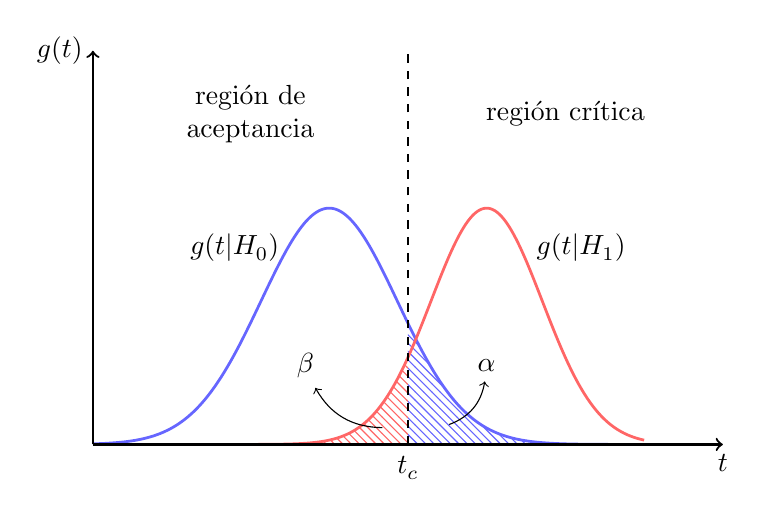
\begin{tikzpicture}

    \colorlet{red}{red!60}
    \colorlet{blue}{blue!60}

    \draw[blue,line width=1] plot[domain=-1:6, samples=500] ({\x},{3*exp(-((\x-2)^2/1.5))});
    \fill[blue, pattern=north west lines, pattern color=blue] (3,0) -- plot[domain=3:6, smooth] ({\x},{3*exp(-((\x-2)^2/1.5))}) -- cycle;

    \draw[red, line width=1] plot[domain=0:6, samples=500] ({\x},{3*exp(-((\x-4)^2)/1)});
    \fill[red, pattern=north west lines, pattern color=red] (3,0) -- plot[domain=0:3,smooth] ({\x},{3*exp(-((\x-4)^2)/1)}) -- cycle;

    \draw[line width=0.8,->] (-1,0) -- (7,0) node[below] {$t$};
    \draw[line width=0.8,->] (-1,0) -- (-1,5) node[left] {$g(t)$};
    %% \draw[line width=0.8] (7,0) -- (7,5);
    %% \draw[line width=0.8] (-1,5) -- (7,5);

    \draw[dashed, line width=0.8] (3, 0) -- (3, 5);
    \draw node at (3,-0.3) {$t_c$};

    \draw node at (0.8, 2.5) {$g(t|H_0)$};
    \draw node at (5.2, 2.5) {$g(t|H_1)$};

    \node[text width=2cm, text centered] at (1, 4.2) {región de aceptancia};
    \node[text width=2.5cm, text centered] at (5, 4.2) {región crítica};

    \draw node (alpha) at (1.7,1) {$\beta$};
    \draw node (p0) at (2.8,0.2) {};
    \draw[->] (p0) edge[bend left] (alpha);

    \draw node (beta) at (4,1) {$\alpha$};
    \draw node (p1) at (3.4,0.2) {};
    \draw[->] (p1) edge[bend right] (beta);

\end{tikzpicture}

\end{figure}

%% Asumiendo que $H_0$ es verdadera, se puede definir una región critica $R$ tal que la probabilidad
%% de que $q$ pertenezca a $R$ sea igual o menor a un cierto valor. El hecho de que $q_\text{obs}$
%% este dentro de $R$, implica que $H_0$ sea rechazada, y de lo contrario aceptada.

%% Primero se define una \emph{región de aceptancia}, tal que si $T(\mathcal{d}) < k_\alpha$
%% uno acepta la hipótesis nula. El contorno $T(\mathcal{d}) = k_\alpha$ delimita el espacio de datos,
%% y es el borde de la región de aceptancia. Se define el tamaño del test, $\alpha$, como la
%% probabilidad de que la hipótesis nula sea rechazada en el caso de ser verdadera (lo que se conoce
%% como error de tipo I). Esto es equivalente a la probabilidad bajo la hipótesis nula de que los datos
%% no sean encontrados en la región de aceptancia, es decir, $\alpha = P(T(\mathcal{D}) \geq k_\alpha|H_0)$

%% En contraste, si uno acepta la hipótesis nula cuando la alternativa es verdadera, es llamado
%% error de tipo II. La probabilidad de cometer este errores la denota $\beta$ y esta dada por
%% $\beta = P(T(\mathcal{D}) < k_\alpha|H_1)$. Se llama \emph{poder del test} a $1-\beta$.

%% Lo que se quiere encontrar es un test estadístico que maximiza el poder del test para un valor
%% fijo de tamaño del test $\alpha$.

La probabilidad de rechazar $H_0$ siendo esta verdadera es,

\begin{equation}
  \alpha =  \int_{R} g(t|H_0)\, dt
\end{equation}
%
y determina el tama\~no del test $\alpha$ o el nivel de significancia del test a
$(100 - \alpha) \%$. El error de rechazar $H_0$ cuando es verdadera es llamado error de tipo I.
Por otro lado el error de aceptar $H_0$ cuando es falsa se llama error de tipo II, y su
probabilidad de ocurrencia ($\beta$), depende de la hipótesis alternativa $H_1$.
El poder del test se define como la probabilidad de rechazar la hipótesis cuando
es falsa:

\begin{equation}
1-\beta = \int_R g(t|H_1)\, dt
\end{equation}

En principio cualquier función de los datos puede ser utilizada como estadístico de prueba. Un buen
estadístico sera aquel para el cual sus distribuciones para la hipótesis nula y alternativa estén
claramente separadas.

Lo que uno quiere es para un dado tama\~no del test, tener el mayor poder posible.
Para el caso de hipótesis simples, el teorema de Neyman-Pearson afirma que el test
con mayor poder dado un tama\~no $\alpha$ esta dado por:

%% Para el caso de dos hipótesis simples (sin parámetros), el test estadístico con mayor
%% poder esta dado por el \emph{likelihood ratio} $T_\text{NP} = \vec{f}(\mathcal{D}|H_1)/\vec{f}(\mathcal{D}|H_0)$.
%% Este resultado se conoce como lema de Neyman-Pearson.


%% Desafortunadamente no hay un equivalente al lema de NP para modelos con muchos parámetros libres.
%% Sin embargo, hay una generelizacion natural basada en el profile likelihood ratio.

\begin{equation}
  t(\bm{x}) = \frac{f(\bm{x}|H_1)}{f(\bm{x}|H_0)}
\end{equation}


Para el caso de un conjunto de datos muy grandes ($N$ grande), la distribución de las medias
de los observables $\bm{x}$ van a seguir una distribución normal incluso si las cantidades
medidas $\bm{x}$ no siguen una distribución normal. Esto es consecuencia del \emph{teorema
  central del limite}. En este caso, la pdf del estadístico de prueba $t$ puede ser
fácilmente determinada. En el caso general, sin embargo, hay que utilizar métodos numéricos y
simulaciones Monte Carlo para determinarla. En ese caso, el conjunto de observables $\bm{x}$ es
generado usando la pdf $f(\bm{x}|H)$ y se calcula el valor del estadístico de prueba $t(\bm{x})$
para cada conjunto. Estos pasos se repiten para acumular estadística en la distribución de
$g(t|H)$.


El nivel de acuerdo entre los datos observados y una dada hipótesis es cuantificado calculando
el \emph{\pvalue}, es decir, la probabilidad, bajo la suposición de que $H$ es cierta,
de observar datos de igual o menor compatibilidad con la predicción de $H$,
respecto a los datos observados.

\begin{equation}
  p_H = P(t>t_\text{obs}|H) = \int_{t_\text{obs}}^{\infty} g(t|H) \, dt
\end{equation}
%
donde $t_\text{obs}$ es el valor del estadístico de prueba obtenido con los datos observados.

De esta forma, un {\pvalue} grande denota que la evidencia en contra de $H_0$ es
débil y un {\pvalue} chico denota que los datos contienen mucha evidencia en contra de $H_0$.
%% En este sentido de p-valores, se puede no hablar de pruebas de hip´otesis, sino de
%% pruebas de significancia, donde la cuantificaci´on del concepto abstracto de significancia
%% es el p-valor

Se dice que la hipótesis es excluida si el {\pvalue} esta por debajo de un valor
especifico dado por el tama\~no del test $\alpha$, donde $\alpha \in [0,1]$.

En física de partículas es usual convertir el {\pvalue} en la signifícancia equivalente, $Z$,
definida como,
\begin{equation}
  Z = \Phi^{-1}(1-p)
\end{equation}
%
donde $\Phi^{-1}$ es el cuantil (la función inversa de la distribución acumulativa) de la distribución
gaussiana.


%% Los modelos de probabilidad pueden construirse para describir simultáneamente varios
%% canales, es decir, varias regiones disjuntas de datos asociadas a un criterio de selección.
%% Si usamos $e$ como el índice sobre eventos y $c$ el índice sobre canales, los datos
%% van a ser una colección de datos: $\mathcal{D}_\text{sim} = {\mathcal{D}_1, \ldots, \mathcal{D}_{c_max}}$.
%% El punto clave ahora, es que va a haber múltiples términos de Poisson.

%% \begin{equation}
%%   \vec{f}_\text{sim} (\mathcal{D}_\text{sim}|\alpha) = \prod_{c \in \text{canales}} \left[ \Pois(n_c|\nu{(\alpha)}) \prod_{e=1}^{n_c} f(x_{c,e}|\alpha) \right]
%% \end{equation}






\section{Descubrimiento}

En general el parámetro de interés es la intensidad de la señal, $\mu$ definida como
$\sigma/\sigma_\text{nominal}$. En el caso de que $\mu = 0$,
tenemos la hipótesis de solo fondo, y cuando vale $\mu = 1$, la hipótesis de señal + fondo.

%% Si $\hat{\mu}$ y $\hat{\btheta}$ son los valores que maximizan $L(\mu,\btheta)$ o minimizan
%% $- \ln L(\mu, \btheta)$ y $\bdtheta$ es el valor que maximiza $L$ para un valor fijo de $\mu$
%% (the profile value of \btheta), el cociente de likelihood es,

%% \begin{equation}
%%   \lambda(\mu) = \frac{L(\mu, \hat{\hat{\bm{\theta}}})}{L(\hat{\mu}, \hat{\bm{\theta}})}
%% \end{equation}
%% %
%% y es independiente de los parámetros \btheta.

Para la búsqueda de una nueva señal solo queremos considerar que los datos
no tengan un buen acuerdo con la hipótesis de solo-fondo solo cuando $\hat{\mu}$
sea mayor a cero. En el caso de experimentos como las oscilaciones de neutrinos
por ejemplo la hipótesis de señal puede predecir un numero mayor o menor de eventos
con respecto a la hipótesis de no oscilaciones.

Aunque es cierto que un valor de $\hat{\mu}$ mucho menor a cero representa evidencia
contra el modelo de solo-fondo, pero este tipo de discrepancia no muestra que los datos
contenga eventos de señal.

Por lo tanto para esta caso de $\mu \geq 0$ conviene definir,

\begin{equation}
  \tilde{\lambda}(\mu) =
  \begin{cases}
    \frac{L(\mu, \hat{\hat{\bm{\theta}}})}{L(\hat{\mu}, \hat{\bm{\theta}})} & \hat{\mu} \geq 0 \\
    \frac{L(\mu, \hat{\hat{\bm{\theta}}})}{L(0, \hat{\bm{\theta}}(0))} & \hat{\mu} < 0
  \end{cases}
\end{equation}

Acá $\dhat{\btheta}(0)$ y $\dhat{\btheta}(\mu)$ se refieren a los estimadores ML de {\btheta} dados
los parámetros de intensidad de señal parámetro de 0 o $\mu$ respectivamente. El correspondiente
estadístico de prueba puede obtenerse como,

\begin{equation}
  \tilde{t}_\mu = -2 \ln \tilde{\lambda}(\mu) =
  \begin{cases}
    -2 \ln \frac{L(\mu, \hat{\hat{\bm{\theta}}})}{L(0, \hat{\bm{\theta}}(0))} & \hat{\mu} < 0 \\
    -2 \ln \frac{L(\mu, \hat{\hat{\bm{\theta}}})}{L(\hat{\mu}, \hat{\bm{\theta}})} & \hat{\mu} \geq 0
  \end{cases}
\end{equation}


\todo{reescribir}Un caso especial importante el estadístico $t_\mu$ es en el caso de $\mu=0$ en un modelo en el que
asumimos $\mu \geq 0$. Rechazar la hipótesis de $\mu=0$ es lo que llamamos \emph{descubrimiento} de
una nueva señal. Para este caso importante definimos $q_0=\tilde{t}_0$. como,

\begin{equation}
  \tilde{q}_0 =
  \begin{cases}
    -2 \ln \tilde{\lambda}(0) & \hat{\mu} > 0 \\
    0 & \hat{\mu} \leq 0
  \end{cases}
\end{equation}

Si los datos fluctúan de tal manera que uno tenga menos eventos que los predichos por
el fondo, entonces $\hat{\mu} = 0$ y tenemos $q_0=0$. A medida que el numero de eventos
crezca por encima del numero de fondo esperado (mayor $\hat{\mu}$) tenemos mayores valores
de $q_0$ que corresponde a un incremento en el nivel de incompatibilidad con la hipótesis
de solo-fondo. Para cuantificar el nivel de desacuerdo entre datos y la hipótesis de
$\mu=0$ usando el valor observado de $q_0$ podemos calcular el valor-$p$ como,

\begin{equation}
  p_0 = \int_{q_{0}^\text{obs}}^{\infty} f(q_0|0) \, dq_0
  \label{eq:p0}
\end{equation}

En el caso de que $p_0 \leq \epsilon$ donde $\epsilon$ es un tamaño del test
prefijado anteriormente, tenemos un descubrimiento. En general en física
de altas energías suele utilizarse $\epsilon = 2.87 \times 10^{-7}$ que corresponde
a una significancia equivalente $Z=5\sigma$.

Es importante hacer notar que el hecho de rechazar la hipotesis de solo-fondo en
un sentido estadistico es solo parte de descrubir un fenomeno nuevo.


\section{Limites de Exclusión}

Si $p_0> \epsilon$, no podemos rechaza $H_0$. Esto no significa que todos los valores de
$\mu$ bajo $H_1$ estén excluidos. Ahora tenemos que testear $H_1[\mu_0]: \mu = \mu_0$ contra
$H_0[\mu_0]: \mu < \mu_0$. Para esto definimos $\tilde{q}_\mu$,

\begin{equation}
  \tilde{q}_\mu =
  \begin{cases}
    -2 \ln \tilde{\lambda}(\mu) & \hat{\mu} \leq \mu \\
    0 & \hat{\mu} > \mu
  \end{cases} \label{eq:qmu}
\end{equation}

Conviene notar que para establecer un limite superior una fluctuación hacia arriba
de los datos no representa una mayor incompatibilidad de la hipótesis $\mu$.

La razón para poner $q_\mu = 0$ para $\hat{\mu} > \mu$ es que cuando seteamos un limite
superior, el hecho de que $\hat{\mu} > \mu$ representa menos compatibilidad con $'mu$ que
los datos obtenidos, y por lo tanto no se considera parte de la región de rechazo del test.

Acá hay que notar, que $q_0$ no es simplemente un caso especial de la {\eq} \eqref{eq:qmu},
sino que tiene una definición diferente. Es decir, $q_0$ es cero si los datos fluctúan
hacia abajo ($\hat{\mu}<0$), pero $q_\mu$ es cero si los datos fluctúan hacia arriba ($\hat{\mu}>\mu$).

Para los datos observados tenemos $\tilde{q}_\mu^\text{obs}$. Para generar la distribución de $\tilde{q}_\mu$
se pueden generar pseudo-experimentos con MC $\to$ $f(\tilde{q}_\mu|\mu, \btheta)$.

El valor-$p$ para una observación bajo una hipótesis $(\mu,\btheta)$ es la probabilidad de obtener
un resultado igual o mas extremo que los obtenidos dada H.

\begin{equation}
  p_{(\mu,\btheta)} = \int_{\tilde{q}_\mu^\text{obs}}^{\infty} f(\tilde{q}_\mu|\mu,\btheta) \, d\tilde{q}_\mu
\end{equation}


Solo nos interesa $\mu$ pero $p$ depende también de $\btheta$. Lo que queremos entonces es
que el valor-$p$ sea chico para todo valor de $\btheta$.

\begin{equation}
  p_\mu^\text{sup} = \sup_\theta p_{(\mu,\btheta)}
\end{equation}

La mayor razón para usar PLR con $t(\bm{x})$ es que en el limite de muchos eventos
la distribución del PLR $\lambda(\mu=\mu_\text{true})$ es independiente de los
valores de los parámetros nuisance $p_\mu^\text{sup} = p_{(\mu,\btheta)} \forall \theta$.
Esto es una consecuencia del teorema de Wilk.


Elegir $\btheta^\text{sup} = \dhat{\btheta}(\mu)$, es decir, el valor para el cual $p_{(\mu,\btheta)} = p_\mu^\text{sup}$
es un buen valor estimado de $\btheta^\text{sup}$.

\begin{equation}
  p_\mu = \int_{\tilde{q}_\mu^\text{obs}}^{\infty} f(\tilde{q}_\mu|\mu,\dhat{\btheta}(\mu, \text{obs})) \, d\tilde{q}_\mu \equiv \clsb
  \label{eq:pmu}
\end{equation}


Para obtener el nivel de confianza estándar de 95\%

\begin{equation}
  p_{\mu_\text{up}} = 0.05
\end{equation}

Para calcular el limite superior {\cls} definimos,\todo{explicar porque \cls}

\begin{equation}
  \cls = \frac{p_\mu}{1-p_b}
\end{equation}
%
donde $p_b$ es el valoro del mismo test bajo la hipótesis de solo-fondo,

\begin{equation}
  p_b = 1 - \int_{\tilde{q}_\mu^\text{obs}}^{\infty} f(\tilde{q}_\mu|0,\dhat{\btheta}(\mu=0)) \, d\tilde{q}_\mu \equiv \clb
\end{equation}


El limite superior {\cls} en $\mu$, $\mu_\text{up}$ se obtiene resolviendo $p_{\mu_\text{up}} = 0.05$.
Se rechazan los valores de $\mu$ si $\mu  < \mu_\text{up}$ con un nivel de confianza de 95\%.


\section{Aproximación asintótica}

Para poder calcular los valores $p$ de una hipótesis utilizando las ecuaciones
\eqref{eq:p0} y \eqref{eq:pmu} necesitamos conocer las distribuciones muestrales del
estadístico de prueba $f(t)$.

En el limite de un gran muestra de datos (limite asintótico) \cite{AsymAprox}, y utiliando el teorema
de Wilks\cite{WilksTheo} y Wald\cite{WaldTheo} es posible escribir la distribución
de $q_0$ completa como,

\begin{equation}
  f(q_0|\mu') = \left( 1 - \Phi\left(\frac{\mu'}{\sigma}\right)\right) \delta(q_0) +
  \frac{1}{2}\frac{1}{\sqrt{2\pi}}\frac{1}{\sqrt{q_0}} \exp \left[ -\frac{1}{2} \left( \sqrt{q_0} - \frac{\mu'}{\sigma} \right)\right]
\end{equation}

Para el caso especial de $\mu' = 0$ la distribución se reduce a:

\begin{equation}
  f(q_0|0) = \frac{1}{2} \delta(q_0) + \frac{1}{2}\frac{1}{\sqrt{2\pi}}\frac{1}{\sqrt{q_0}} e^{-q_0/2}
\end{equation}

En el limite de la gran muestra, $f(q_0|0)$ es independiente de los parámetros nuisance,
aunque $f(q_0|\mu')$ depende de los parámetros nuisance a través de $\sigma$.

De la pdf, la distribución acumulada de $q_0$ es,

\begin{equation}
  F(q_0|\mu') = \Phi \left( \sqrt{q_0} - \frac{\mu'}{\sigma} \right)
\end{equation}

Para el caso especial $\mu' = 0$ es $F(q_0|0) = \Phi(\sqrt{q_0})$ y el valor-$p$
de la hipótesis $\mu=0$ es

\begin{equation}
  p_0 = 1 - F(q_0|0)
\end{equation}

y la significancia de descubrimiento $Z$ es simplemente,

\begin{equation}
  Z = \Phi^{-1} (1-p_0) = \sqrt{q_0}
\end{equation}


La distribución de $q_\mu$ en este mismo limite es,

\begin{equation}
  f(q_\mu|\mu') = \Phi\left(\frac{\mu'-\mu}{\sigma}\right) \delta(q_\mu) +
  \frac{1}{2}\frac{1}{\sqrt{2\pi}}\frac{1}{\sqrt{q_0}} \exp \left[ -\frac{1}{2} \left( \sqrt{q_\mu} - \frac{\mu'-\mu}{\sigma} \right)^2\right]
\end{equation}


\section{Significancia esperada} %%Sensibilidad de descrubrimiento para un experimento de conteo}

When planning the experiment, we want to quantify how sensitive
we are to a potential discovery, e.g., by given median significance
assuming some nonzero strength parameter mu'.
%% So for p-value, need f(q0 |0), for sensitivity, will need f(q0 | mu'),


En física de partículas la cantidad $s/\sqrt{b}$ ha sido siempre utilizado como
una medida de la significancia esperada de descubrimiento. La explicación detrás
de esta formula es que una cantidad $n$ que sigue la distribución de Poisson con
una media grande $s+b$ puede ser aproximada por una variable $x$ distribuidas según
una gaussiana con media $s+b$ y desviación estándar $\sqrt{s+b}$. En este caso
el valor-$p$ de la hipótesis de solo-fondo dada una observación $x$ esta dado por,

\begin{equation}
  p = 1 - \Phi \left( \frac{x-\mu}{\sigma} \right) = 1 - \Phi \left( \frac{x-b}{b} \right)
\end{equation}
%
donde $\mu=b$ y $\sigma = \sqrt{b}$ se refieren a la media y la desviacion estandar de x
asumiendo que $s=0$. Traduciendo este valor-$p$ a significancia,

\begin{equation}
  Z = \frac{x-b}{b}
\end{equation}

La significancia esperada es entonces (ya que la media es $s+b$)

\begin{equation}
  Z_\text{esperada} = \frac{s}{\sqrt{b}}
  \label{eq:Zsimple}
\end{equation}

Si el numero esperado de eventos de fondo $b$ es conocido con una incerteza despreciable,
entonces la funcion likelihood es,

\begin{equation}
  L(s) = \frac{(s+b)^n}{n!} e^{-(s+b)}
\end{equation}

Utilizando la aproximacion asintotica descripta anteriormente, la significancia de descubrimiento
puede ser aproximada por $Z=\sqrt{q_0}$, lo que para este problema daria,

\begin{equation}
  Z = \sqrt{2\left( n \ln \frac{n}{b} +b -n \right)}
  \label{eq:Z}
\end{equation}
%
para $n>b$ y $Z=0$ sino. Tambien puede aproximarse la significancia esperada reemplazando los datos
por el conjunto de datos de Asimov. Substituyendo $s+b$ por $n$ en la {\eq} \eqref{eq:Z}, la aproximaxion de
Asimov para la significancia esperada $Z_A$ es,

\begin{equation}
  Z_A = \sqrt{2\left( (s+b) \ln \left( 1 + \frac{s}{b}\right) - s \right)}
\end{equation}

Si expandimos el logaritmo en la ecuaciona anterior en $s/b$ tenemos $Z_A = s/\sqrt{b} + \mathcal{O}(s/b)$
que es la expresion de la {\eq} \eqref{eq:Zsimple} y es valida solo en el limite $s \ll b$.

Si el numero de eventos esperado de fondo $b$ no es conocido, uno debe incluirlo como
un parametro nuisance en la funcion likelihood. Pero como $b$ puede ajustarse para cualquier
numero de evenots, es necesario introducir informacion adicional para constrain $b$. En general
se suele hacer mediante una medida auxiliar, mirando el numero de evnetos observados $m$ en una
region de control donde se asume que la senal esta ausente, y se puede considerar que $m$ sigue
una distribucion de Poisson con media $\tau b$, donde $\tau$ es un factor \fix{extrapolacion}.

La funcion likelihood total es el producto de las dos distribuciones de Poisson correspondientes
a cada region:

\begin{equation}
  L(\mu, \btheta) = \Pois_\text{SR}(n;s+b) \Pois_\text{CR}(\tau b)
\end{equation}

Utilizando la aproximacion $Z = \sqrt{q_0}$, valida en el limite de una gran muestra y
teniendo en cuenta que los valores esperados son $s+b$ y $\tau b$ para obtener la significancia
mediana, tenemos

\begin{equation}
  Z_A = \left[ 2 \left( (s+b) \ln \left[ \frac{s+(1+\tau)b}{(1+\tau)(s+b)} \right] + \tau b  \ln \left[ 1 + \frac{s}{(1+\tau)b} \right] \right) \right]^{1/2}
  \label{eq:Za1}
\end{equation}

Es util expresar la {\eq} \eqref{eq:Za1} en terminos de la incerteza que uno quiere
atribuirle al fondo basados en la medida de control $m$. El estimador para $b$ esta dado
por $\hat{b} = m/\tau$, y como la varianza de $m$ es igual a su media $\tau b$, la
varianza de $\hat{b}$ es $V[\hat{b}] = \sigma_b^2 = b/\tau$. Y usando esto para eliminar
$\tau$ de la {\eq} \eqref{eq:Za1} obtenemos:

\begin{equation}
  Z_A = \left[ 2 \left( (s+b) \ln \left[ \frac{(s+b)(b+\sigma_b^2)}{b^2+(s+b)\sigma_b^2} \right] - \frac{b^2}{\sigma_b^2} \ln \left[ 1 + \frac{\sigma_b^2 s}{b(b+\sigma_b^2)} \right] \right) \right]^{1/2}
  \label{eq:Za}
\end{equation}

%% \subsection{Psuedo-experimentos}

%% The role of intervals in Search Procedures

%% Exclusion A signal hypothesis can be excluded if the compatibility with the s C b
%% hypothesis is ‘small’. Several limit-setting methods exist and are a source of in-
%% tense discussions among physicists, to say the least (see also Section 4.6). Although
%% it might seem natural to define a signal as excluded at 95% confidence level if
%% CL sCb < 5%, there are some undesirable consequences associated with this choice.
%% Near the sensitivity limit, where the test statistic distribution for the b-only and sCb
%% hypotheses are not well separated (either because the signal is small or the analysis
%% is not powerful enough to separate signal and background), a downward fluctua-
%% tion in the data with respect to the b-only expectation will result in the exclusion
%% of a signal while the analysis has no real sensitivity. One of the common solutions

%% experiments invoke to address this issue is to correct for a downward fluctuation
%% by using the so-called CL s method [6], where a signal is called ‘excluded’ at 95%
%% confidence level if CL s < 0.05, where CL s


%% Para ilustrar el uso del likelihood ratio, consideremos un experimento en el cual por cada evento,
%% se miden los valores de ciertas variables cinematicas, entonces los datos pueden ser representados
%% por uno o mas histogramas.

%% Supongamos el histograma $\vec{n} = (n_1, n_2, \ldots, n_n)$. El valor esperado para $n_i$ puede
%% escribirse $E[n_i] = \mu s_i + b_i$, donde el valor medio de entradas del bin $i$ de se\~nal y fondo
%% son:

%% El parametro $\mu$ determina la intensidad de la nueva se\~nal, donde $\mu=0$ corresponde a la
%% hipotesis de solo-fondo, y $\mu=1$ es la hipotesis de se\~nal.
%% Las funciones $f_s$ y $f_b$ son las \pdf\ de la variable x para los eventos de se\~nal y fondo, y
%% $\theta_s$ y $\theta_b$ representan parametros que caracterizan la forma de las pdfs. Las
%% cantidades $s_\text{tot}$ y $b_\text{tot}$ son el valor medio total de se\~nal y fondo, y las
%% integrales en \ref{} y \ref{} representan la probabilidad de que un evento sea encontrado en el
%% bin $i$. En lo que sigue $\bm{\theta} = (\bm{\theta}_s, \bm{\theta}_b, b_\text{tot})$

%% Además del histograma $\bm{n}$, se utilizan otras medidas adicionales que ayuden a restringir
%% los parametros nuisance. Por ejemplo, se pueden elegir regiones de control donde uno espera
%% mayormente fondo, y construit un histograma $\bm{m}$. Los valores esperados de $m_i$ pueden
%% escribirse como $E[m_i] = u_i(\bm{\theta})$, donde los $u_i$ son cantidades calculadas a partir
%% de $\bm{\theta}$.

%% \itodo{
%%   It is often said that the language of science is mathematics. It could well be said that the language of experimental science is statistics.
%%   It is through statistical concepts that we quatify
%%   the correspondence between theoretical predicticions and experimental observations. While the statistical
%%   analysis of the dta is often treated as a final subsidiary step to an experimental physcis
%%   result, a more direct approach would be quite the opposite. In fact, thinking through the
%%   requirements for a robust statistical statement is an excellent way to organize an analysis
%%   strategy.
%%   }





%% \subsection{Probabilidad}

%% La definición matemática de probabilidad

%% Consideremos A un evento. Luego la probabilidad $P(A)$ es un numero que obedece los tres
%% axiomas de Kolmogorov\cite{Kolmogorov}.

%% \begin{align}
%%   &P(A) \geq 0, \\
%%   &P(S) = 1, \\
%%   &A \cap B = \phi \Rightarrow P(A \cup B) = P(A) + P(B)
%% \end{align}
%% %
%% donde $S$ es el conjunto de A.

%% La definición frecuentista de probabilidad esta dada por:

%% \begin{equation}
%%   P(A) = \lim_{n\to\infty} \frac{\text{resultado es} A}{n}
%% \end{equation}


%% \begin{equation}
%%   P(A|B) = \frac{P(B|A) P(A)}{P(B)}
%% \end{equation}
%% %
%% donde $P(B|A)$ es la probabilidad de B dado A, $P(A)$ es la probabilidad \emph{a priori} de A,
%% y ...

%% \chapter{Estrategia general del análisis}
\label{cap:estrategia}

En el \cref{cap:estadistica} se describieron los conceptos básicos de estadística
necesarios para realizar un análisis de búsqueda de nueva física. En este
capítulo, haciendo uso de estos conceptos, se describe la estrategia general
y la construcción del modelo estadístico utilizado en el presente análisis.


\section{Estrategia, señal y fondos del SM}

El análisis realizado para esta tesis consiste en la búsqueda de Supersimetría en
eventos con un fotón aislado muy energético, jets y gran cantidad de energía
faltante. La estrategia general consistió en realizar un experimento de conteo,
es decir, considerar como variable estadística al número de eventos observado en
una cierta región del espacio de observables, rica en eventos de la señal considerada.
Un experimento de conteo puede
pensarse en el contexto del \emph{likelihood} extendido, \cref{eq:likelihood_ext}, con
$f(x) = 1$, el cual se reduce solo al término de Poisson.

El mayor desafío para poder realizar cualquier descubrimiento de nueva física es
entender los procesos del SM que pueden dar lugar a un estado final que emule
la señal buscada (fondos).
En este caso van a ser los que tienen un fotón, jets y energía faltante en el estado final.
Estos pueden dividirse en varias categorías.
Por un lado, los procesos que dan lugar a eventos con un fotón y energía
faltante real, es decir, los que llamamos fondos irreducibles. Estos son:

\begin{itemize}
\item $Z(\to\nu\nu)+\gamma$
\item $W(\to l\nu)+\gamma$
\item $t\bar{t}+\gamma$
\end{itemize}
%
También es posible que, aunque el proceso no tenga fotones en el estado final, un
electrón o un jet sean identificados como un fotón, dando lugar a un estado final
idéntico al buscado. En esta categoría están:

\begin{itemize}
\item $W(\to l\nu)$ + jets
\item $Z(\to \nu\nu)$ + jets
\item $t\bar{t}$
\item $WW$, $ZZ$, $WZ$
\end{itemize}

Y por último, también puede haber procesos que a pesar de no generar energía
faltante real, poseen lo que se denomina energía faltante instrumental,
proveniente generalmente de la incorrecta reconstrucción de la energía de los
jets. De esta manera, pueden dar lugar a eventos con el estado final de interés,
los procesos QCD:

\begin{itemize}
\item $\gamma+$jets
\item multijet, con alguno de los jets identificado como fotón
\item $Z(\to ll)+$jets, donde un leptón o un jet es identificado como un fotón.
\end{itemize}

%% En el \cref{cap:simulaciones} se describen como estos procesos del SM son
%% simulados utilizando generadores Monte Carlo. Aunque en general, para el LHC,
%% las predicciones de las simulaciones Monte Carlo no son lo suficientemente
%% precisas, ya que nunca fueron testeadas a energías tan altas. Por este motivo
%% resulta necesario desarrollar técnicas de estimación de los fondos utilizando los
%% propios datos observados. Estos métodos se describen en el \cref{cap:fondos}.

%% Es indispensable para el análisis contar con predicciones de los procesos
%% fisicos conocidos como los de nueva fisica en esta región, para lo cual resulta fundamental
%% la simulación de los mismos. Para ello se utilizan generadores Monte Carlo y
%% una detallada simulación del detector, seguidamente de la reconstrucción con los mismos
%% algoritmos utilizados en los datos de colisiones.
%% Adicionalmente, la contribución de algunos fondos pueden ser estimada utilizando
%% métodos basados únicamente en los datos.

%% En el caso de que el número de eventos observado sea compatible con el número de
%% eventos esperado debido a procesos del SM, pueden establecerse límites en la
%% sección eficaz de nueva física.

Otro componente importante del análisis es la simulación de los procesos de
señal. Las muestras de señal pueden depender de uno o muchos parámetros del
modelo considerado, como por ejemplo de las masas de las nuevas partículas
predichas por Supersimetría. En el caso de considerar un espacio
multidimensional del espacio de parámetros del modelo, se utiliza una
<<\emph{grid}>> de escenarios de señal, en la que cada punto de la \emph{grid}
corresponde a un único punto en el espacio de parámetros. En particular en esta
tesis, se consideró un modelo de Supersimetría que puede dar lugar a este tipo
de estados finales, para lo cual es necesario contar con la simulación de la
señal considerada. En el caso de que no se observe un exceso de eventos en los
datos, se pueden establecer límites de exclusión en la \emph{grid}, excluyendo
un subconjunto de los valores de los parámetros considerados.


%---------------
% Regiones
%---------------
\section{Regiones de señal, control y validación}
\label{sec:regiones}

%---------------
% Signal Region
%---------------
Un análisis en el que se quiera estudiar un determinado fenómeno de nueva física
requiere la definición de una región en el espacio de observables, donde el modelo de señal
predice un exceso significativo de eventos sobre el nivel de fondo predicho en
la misma región. A esta región enriquecida en señal se la llama región de señal
(SR).

%-----------
% Fondos/CR
%-----------
Una de las tareas fundamentales del análisis es entonces, estimar las
contribuciones de los procesos del SM que contaminan la región de
señal.
Para esto existen dos técnicas principales: utilizar directamente simulaciones Monte Carlo,
o utilizar métodos basados en los propios datos observados.

%% La primera de las técnicas consiste en generar una gran cantidad de eventos
%% utilizando técnicas de Monte Carlo del proceso físico considerado. En general
%% este proceso se realiza en varias etapas. Con un generador de eventos se realiza
%% la simulación de la interacción fuerte (por ej. {\madgraph}). Luego con el mismo
%% u otro generador se realiza la lluvia de partones y el proceso de hornecino
%% (por ej. {\pythia}). Y finalmente se simula la interacción de las partículas
%% generadas con el detector ({\geant}). A cada proceso que se simula de esta forma
%% lo llamaremos muestra en referencia a la muestra correspondiente generada con
%% Monte Carlo.

%% Para cada proceso físico tenemos que el número de eventos esperado por unidad de
%% tiempo (tasa) estará dado por:

%% \begin{equation}
%%   \text{tasa} = (\text{flujo}) \times (\text{sección eficaz}) \times
%%   (\text{eficiencia}) \times (\text{aceptancia})
%% \end{equation}
%% %
%% donde la sección eficaz esta predicha por la teoría, el flujo es controlado por
%% el acelerador, y la eficiencia y la aceptancia son propiedades del detector y
%% los criterios de la selección de eventos. Esta relación no es más que la
%% refórmalo invariante de la probabilidad de dispersión predicha por primeros
%% principios de la mecánica cuántica $P(i\to f) =
%% |\braket{i}{f}|^2/(\braket{i}{i}\braket{f}{f})$.

%% Si llamamos seccion eficaz efectiva $\sigma_\text{eff}$ al producto de la
%% sección eficaz, la eficiencia y la aceptancia, el número de eventos esperado
%% para un dado proceso ($\nu$) va a ser el producto de la luminosidad integrada en
%% el tiempo $L$ y la sección eficaz efectiva:

%% \begin{equation}
%%   \nu = L \sigma_\text{eff}
%% \end{equation}

%% Sin tener en cuenta los efectos del detector, la distribución de un observable
%% $x$ sera

%% \begin{equation}
%%  f(x) = \frac{1}{\sigma_\text{eff}} \frac{d\sigma_\text{eff}}{dx}
%% \end{equation}

%% Como ya hemos simulado el pasaje de las partículas por el detector podemos
%% estimar la distribución subyacente $f(x)$ creando un histograma del observable
%% $x$ con la muestra simulada.

La validez de la simulaciones MC está fundamentalmente relacionada a cómo la
teoría subyacente modela las observaciones experimentales. Las debilidades de la
estimación del fondo a partir de las simulaciones derivan de las debilidades de
los modelos teóricos propiamente dichos. En este caso existe una motivación para
utilizar métodos que puedan dar una estimación de los fondos a partir de los
datos experimentales. Existen distintas formas para estimar un fondo a partir de
los datos observados. En el \cref{cap:fondos} se describirán los métodos
específicos utilizados en este análisis.

En algunos casos se emplea un tercer método para estimar los fondos, que consiste en
utilizar la estimación proveniente de las simulaciones MC, pero corregida
a partir de los datos. Para esto se define una región de control (CR) en
la cual el fondo dominante pueda ser controlado comparándolo con los datos
observados en esa misma región. Las CR son diseñadas especialmente para tener
una alta pureza en uno de los procesos de fondo y deben estar libres de
contaminación de señal.

A través del ajuste a los datos, el número de eventos observado en una CR es
usado para normalizar el número de eventos estimado de fondo en todas las
regiones, especialmente en la SR. Es decir, las predicciones iniciales de las
simulaciones MC son llevadas al nivel observado en la correspondiente CR,
usando un factor de normalización calculado en el ajuste. Este factor es
utilizado entonces en la extrapolación a las demás regiones.

%--------------------
% Validation regions
%--------------------
Otro componente importante del análisis es la validación del método utilizado
para predecir los fondos en las SR. Con este objetivo se definen regiones de
validación (VR) que se encuentren entre las CR y las SR en términos de los
principales observables cinemáticos en los criterios de selección. El diseño de
las VR comprende un compromiso entre minimizar la contaminación de la señal, y a su
vez ser efectivas en la validación de la extrapolación entre CR y SR. En la
\cref{fig:regions_sketch} se puede ver un esquema de las regiones descriptas
anteriormente.

\begin{figure}[!htbp]
  \centering 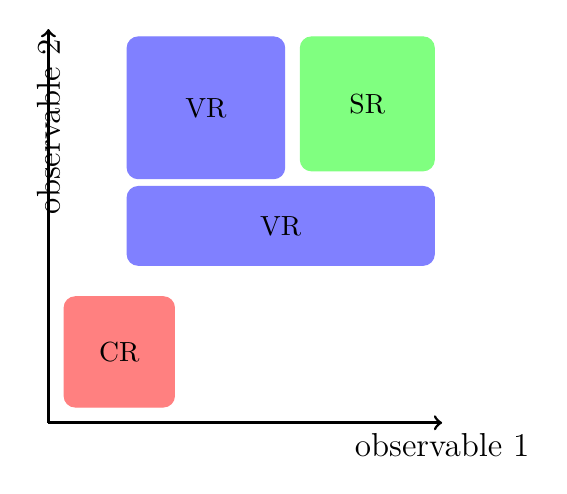
\begin{tikzpicture}

    \tikzstyle{region} = [rounded corners, fill]

    \colorlet{red}{red!50}
    \colorlet{blue}{blue!50}
    \colorlet{green}{green!50}

    \draw[line width=1, ->] (0,0) -- (5,0) node[below] {\large observable 1};
    \draw[line width=1, ->] (0,0) -- (0,5) node[left, rotate=90] {\large observable 2};

    %\draw[dashed, line width=0.8] (5, 0) -- (5, 7);
    %\draw node at (5,-0.3) {\large $t_c$};

    %\draw node at (1.5, 4) {\large $g(t|H_0)$};

    \draw[region, red] (0.2,0.2) rectangle (1.6,1.6) node[midway,black] {CR};

    \draw[region, green] (3.2,3.2) rectangle (4.9,4.9) node[midway,black] {SR};

    \draw[region, blue] (1,2) rectangle (4.9,3) node[midway,black] {VR};
    \draw[region, blue] (1,3.1) rectangle (3,4.9) node[midway,black] {VR};


    %\draw node (alpha) at (3,-0.5) {\large $\beta$};
    %\draw node (p0) at (4.7,0.5) {};
    %\draw[->] (p0) edge[bend left] (alpha);

    %\draw node (beta) at (7,-0.5) {\large $\alpha$};
    %\draw node (p1) at (5.1,0.2) {};
    %\draw[->] (p1) edge[bend right] (beta);

\end{tikzpicture}

  \caption{Esquema del diseño de las regiones de señal (SR), control (CR) y
    validación (VR) en términos de dos observables arbitrarios.}
  \label{fig:regions_sketch}
\end{figure}

Es importante que las CR, VR y SR sean estadísticamente independientes para
poder combinar la pdf que modela cada región en una pdf conjunta. Esto es
fundamental ya que al ajustar los parámetros de la función \emph{likelihood} se deberá
hacer un ajuste simultáneo, que es importante para poder compartir los
parámetros de los fondos y las incertezas sistemáticas entre las distintas
regiones de forma consistente.


%------------------------
% Extrapolacion CR -> SR
%------------------------
\section{Extrapolación y factores de transferencia}

Una de las suposiciones realizada en la sección anterior fue que las variables
cinemáticas que se usan para diferenciar CR y SR están bien modeladas después de
haber ajustado la pdf total a los datos en las CR. Una vez que los procesos de
fondo dominantes son normalizados en las CR, las correspondientes modificaciones
en la pdf pueden ser extrapoladas a las VR, las cuales son utilizadas para
verificar la validez de esta suposición inicial. Solo cuando se demuestra el
acuerdo entre las predicciones del fondo normalizadas y los datos observados en
las VR, las predicciones del fondo son extrapoladas a las SR.
Es en este paso que los datos observados en las SR son considerados por primera
vez para el análisis. Este proceso es llamado <<\emph{unblinding}>> y es
utilizado para adquirir confianza en los métodos usados y
evitar el uso de predicciones prematuras y un posible sesgo en el
resultado final.

En este procedimiento se utilizan de forma implícita los
denominados <<factores de transferencia>>, como se explica a continuación.
Las predicciones de los fondo normalizadas en el ajuste son:

\begin{align}
  N_p^{\text{est}}(\text{CR}) &= \mu_p \times \text{MC}_p (\text{CR})
  \\ N_p^{\text{est}}(\text{SR}) &= \mu_p \times \text{MC}_p (\text{SR})
\end{align}
%
donde $N_p^{\text{est}}(\text{CR})$ y $N_p^{\text{est}}(\text{SR})$ es el número
de eventos estimado para cada proceso de fondo $p$ y
$\text{MC}_p^{\text{est}}(\text{CR})$ y $\text{MC}_p^{\text{est}}(\text{SR})$ es
el número de eventos obtenido de las simulaciones MC. El factor $\mu_p$ es el
factor de normalización obtenido en el ajuste a datos.

Definiendo $N_p^\text{fit}(\text{SR})$ como el valor ajustado en la CR, se puede
escribir de forma equivalente:

\begin{align}
  N_p^\text{est}(\text{SR}) &= \mu_p \times \text{MC}_p (\text{SR}) \nonumber \\
  &\equiv N_p^\text{fit}(\text{CR}) \times \left[ \frac{\text{MC}_p(\text{SR})}{\text{MC}_p(\text{CR})} \right]
\end{align}

El cociente que aparece dentro de los corchete es llamado factor de
transferencia (TF). Un aspecto importante de los TF es que las incertezas
sistemáticas de los valores estimados de fondo pueden ser parcialmente
canceladas en la extrapolación. La incerteza total en el número de eventos de
fondo en la SR es por lo tanto una combinación de las incertezas estadísticas en
las CRs y la incerteza sistemática residual de la extrapolación. Por esta razón
las CR suelen definirse con una selección un poco más relajada, para incrementar
la estadística, sin aumentar significativamente la incerteza en los TF, y así
reducir las incertezas en la SR.


%--------
% Modelo
%--------
\section{Construcción del modelo estadístico}

%% El modelo, que es simplemente una familia de pdfs despcripta por un número finioto
%% de parametros, describe la prediccion nominal (junsto con sus variaciones sistematicas
%% asociadas) de las multiples senales y procesos de fondo en las multiples regiones.

%% El modelo estadistico (la pdf)  tiene que contenter el parámetro de interés (la intensidad
%% de la señal $\mu_s$), los factores de normalización para los procesos de fondo, y los
%% llamados parámetros nuisance que modelan el impacto de las incertezas
%% sistemáticas. Cada incerteza sistemática $i$ se describe con un parámetro
%% nuisance $\theta_i$ que interpola entre el valor nominal y las variaciones de
%% las incertezas sistemáticas.

%% Es decir para las variaciones de las incertezas
%% sistemáticas $\pm \sigma$ tenemos $\theta_i = \pm 1$ y $\theta_i = 0$ para el
%% valor nominal.

La función \emph{likelihood} general para un experimento de conteo como el que se utiliza
en el análisis de esta tesis es el producto de los términos de Poisson del
número de eventos en la SR y las CR, y una distribución adicional que implementa
las restricciones en las incertezas sistemáticas. Puede escribirse como:

\begin{align}
  L(\mu_s, \bm{\mu}_p, \btheta) &= \mathcal{P}_\text{SR} \, \cdot \, \mathcal{P}_\text{CR} \, \cdot \, \mathcal{C}_\text{syst} \nonumber \\
  &= \Pois(n|\lambda(\mu_s, \bm{\mu}_p, \btheta)) \, \cdot \, \prod_{i \,\in\, \text{CR}} \Pois(n_i|\lambda_i(\mu_s, \bm{\mu}_p, \btheta)) \, \cdot \, \mathcal{C}_\text{syst} (\btheta^0, \btheta) \label{eq:model}
\end{align}
%
Los primeros dos factores ($\mathcal{P}_\text{SR}$ y $\mathcal{P}_\text{CR}$)
reflejan las distribuciones de Poisson de $n$, $n_i$, el número de eventos observado
en cada región. Los valores esperados de las distribuciones de Poisson $\lambda_i$ son
funciones que dependen de las predicciones de señal y los distintos fondos $p$,
los parámetros \emph{nuisance} que parametrizan las incertezas sistemáticas $\btheta$,
los factores de normalización para los procesos de fondo $\bm{\mu}_p$ y también
la intensidad de la señal $\mu_s$. Para $\mu_s = 0$ se tiene la
función \emph{likelihood} para la hipótesis de solo-fondo y con $\mu_s = 1$ el
valor esperado de señal.

Las incertezas sistemáticas son incluidas usando la pdf
$\mathcal{C}_\text{syst}(\btheta^0, \btheta)$, donde $\btheta^0$ son los valores centrales
de las medidas auxiliares alrededor de los cuales $\btheta$ puede variarse al
maximizar el \emph{likelihood}. El impacto de los cambios en los parámetros \emph{nuisance}
en los valores esperados están completamente descriptos por las funciones que
predicen la cantidad de señal y fondo, $\lambda_i$. Para parámetros \emph{nuisance}
independientes $\mathcal{C}_\text{syst}$ es simplemente el producto de las pdf
correspondientes a las mediciones auxiliares que describen cada una de las
incertezas sistemáticas, típicamente una distribución gaussiana $G$ con ancho
unidad,

\begin{equation}
  \mathcal{C}_\text{syst} (\btheta^0, \btheta) = \prod_{j \in \text{S}} G(\theta_j^0 -
  \theta_j)
\end{equation}
%
donde $S$ es el conjunto completo de las incertezas sistemáticas consideradas. Las
medidas auxiliares $\theta^0_j$ son típicamente fijadas a cero, pero pueden
variar cuando se generan los pseudo-experimentos.


\section{Ajuste del modelo y resultados}

A partir del modelo general descripto en la sección anterior, \cref{eq:model},
se pueden realizar distintos tipos de ajuste, dependiendo de las regiones utilizadas
y si se incluyen o no las muestras de señal.

Como primer paso se realiza el ajuste únicamente utilizando las regiones de
control, y sin incluir las muestras de señal. El propósito de este ajuste es
estimar el fondo total esperado en las regiones de validación y las regiones de
señal, sin hacer ningún tipo de suposición en algún modelo de señal. Solo se
incluyen las muestras de fondo, y las CR se suponen en libres de contaminación
de señal. El ajuste se realiza utilizando la \cref{eq:model} sin el término de
la SR, y las contribuciones de los procesos de fondo dominantes se normalizan al
número de eventos observados en esas regiones. A partir de los parámetros del
ajuste se puede predecir el número de eventos de fondo en SR y VR. Estas
predicciones de fondo son independientes del número de eventos observado en la
SR (y VR) ya que solo las CR se usan en el ajuste. Esto permite una comparación
no sesgada entre las predicciones y el número de eventos observado en esas
regiones.
A partir de este ajuste es posible ver si existe un exceso de datos respecto al
fondo del SM en las SR, y cuantificar ese exceso calculando el {\pvalue} y la significancia
del mismo.

En ausencia de un exceso de eventos significativo, para poder establecer límites
en la señal, se incluyen en el modelo las regiones de señal. El ajuste se realiza
entonces simultáneamente en las CR y SR, incorporando la muestra de señal
en todas las regiones a fin de tener en cuenta la posible contaminación de
señal en las CR. Este ajuste se realiza de forma independiente para cada SR, y
se repite por cada punto de señal de la \emph{grid}, para probar el espacio de
parámetros del modelo, y establecer límites en las masas de las partículas
supersimétricas consideradas.

%% \chapter{Modelo de señal y generación de eventos Monte Carlo}
\label{cap:simulaciones}

La simulación de los distintos procesos físicos y la respuesta del detector a
los mismos es necesaria para poder optimizar y estimar el desempeño de los
diferentes análisis. Además, permite que las estrategias utilizadas en la
identificación de partículas puedan ser desarrolladas con anterioridad y las
eficiencias de los algoritmos pueden ser puestos a prueba. La preparación de las
búsquedas de nueva física necesitan una simulación detallada del detector para
estimar su potencial de descubrimiento y para desarrollar métodos optimos para medir las
propiedades de las partículas. Es fundamental un correcto entendimiento de los
procesos de señal y de fondo para poder distinguir entre ambos. Una vez que los
datos de colisiones reales están disponibles, los datos simulados también
resultan necesarios tanto para poder encontrar desviaciones del SM.

La estructura de los eventos de colisiones de altas energías son realmente
complejos y no predecibles de primeros principios. Los generadores de eventos
permiten separar el problema en varios pasos más simples, algunos de los cuales
pueden ser descriptos por primeros principios, y otros necesitan ser basados en
modelos apropiados con parámetros ajustados a los datos. Un aspecto central de
los generadores es que proveen una descripción del estado final para
poder construir cualquier observable y compararlos con los datos de colisiones
reales.

En este capítulo se describe como fueron simulados los procesos del modelo de
SUSY (\cref{sec:sig_samples}) y los procesos del SM (\cref{sec:bkg_samples}) que
dan lugar al estado final de interés. Todas las muestras fueron simuladas
utilizando generadores Monte Carlo a $\sqrt{s}=8\tev$, a continuación se simuló
el pasaje de las particulas generadas por el detector ATLAS, para finalmente ser
reconstruidas con los mismos algoritmos que los datos de colisiones reales.


\section{Generación de eventos Monte Carlo}

La conexión entre la teoría/fenomenología de SUSY (o cualquier otra teoría de
nueva física), y los datos observados en el detector de un colisionador se
realiza por medio de un <<generador de eventos Monte Carlo>>
\cite{Sjostrand:2006su,Dobbs:2004qw}. Dada una teoría de nueva física, que en
general predice la existencia de nuevas partículas y/o interacciones, el
generador de eventos permite calcular cómo esa teoría se manifestará en el
experimento.

El procedimiento, una vez que se selecciona un modelo particular de SUSY,
requiere de varios pasos que se encuentran esquematizados en la
\cref{fig:mc_sketch} \cite{Baer:2009tk}. En primer lugar es necesario calcular
el espectro de masas de las partículas supersimétricas, y sus acoplamientos. A
partir de ellos se calculan los anchos y tazas de decaimiento de todas estas
partículas, y por último se utiliza el generador de eventos, que toma como entrada las
masas y decaimientos calculados previamente, y genera un conjunto de eventos a
la energía de centro de masa del colisionador. A continuación, para cada evento,
se simula el pasaje de las partículas por el detector.

Para las distintas etapas suelen
utilizarse herramientas diferentes, por lo que es fundamental contar con un
forma estandarizada de intercambio de información entre ellas. Con este objetivo
se creó un tipo de archivo llamado SLHA (\emph{SUSY Les Houches Accord})\cite{SLHA} que
permite organizar toda la información de un cierto modelo de supersimetría
(parámetros, masas, decaimientos) en un formato único, de modo que sea fácil de
compartir entre los físicos y también entre las distintas herramientas
utilizadas.

\begin{figure}[!htbp]
  \centering

  \scalebox{0.71}{\begin{tikzpicture}[node distance=1.5cm, auto,]

    \node[rec] (susy) {\sc Modelo SUSY};
    \node[rec, right=of susy] (masses) {\sc Espectro de Masas};
    \node[rec, right=of masses] (decays) {\small \sc Decaimientos};
    \node[rec, right=of decays] (gen) {\sc Generador de Eventos};
    \node[rec, right=of gen] (atlas) {\sc Simulación Detector};

    \draw[arr] (1.7,0) -- (2.7,0);
    \draw[arr] (6.2,0) -- (7.2,0);
    \draw[arr] (10.8,0) -- (11.7,0);
    \draw[arr] (15.1,0) -- (16.1,0);

\end{tikzpicture}
}

  \caption{Etapas de la simulación de eventos de un modelo particular de SUSY.}
  \label{fig:mc_sketch}
\end{figure}


\subsection{Espectro de masas y decaimientos}

Los modelos de SUSY que se estudian en el LHC suelen ser la teoría efectiva a
bajas energías que resulta de una teoría más general, como teoría de
supercuerdas, o que involucre un mecanismo particular para el rompimiento de
SUSY. Para especificar una teoría efectiva es necesario definir: la simetría de
gauge, los campos que la componen y el lagrangiano. Como se describió en el
\cref{cap:susy}, los efectos del rompimiento de SUSY están codificados en los
términos de rompimiento \emph{soft} del lagrangiano. También es necesario especificar
la escala de energía a la cual la teoría efectiva y el lagrangiano son válidos.
Como los experimentos prueban física a la escala del {\tev}, mientras que los
parámetros del lagrangiano son frecuentemente especificados a energías mucho más
altas ($M_\text{GUT}$ o $M_P$), deben usarse las ecuaciones del grupo de
renormalización (RGE) para conectar las dos escalas del modelo. Una vez que los
parámetros del lagrangiano son conocidos a la escala electrodébil, pueden
identificarse las masas físicas de las partículas, diagonalizando las matrices
de masa correspondientes, y luego, para tener la precisión suficiente, aplicar
las correcciones a ordenes mayores (en general a 1 \emph{loop}). A partir del modelo
también es posible calcular los anchos y tasas de decaimiento de todas las
partículas supersimétricas.

Existe una gran variedad de programas que permiten realizar estos cálculos. En
este trabajo se utilizó el programa {\susyhit}\cite{Djouadi:2006bz} que combina
{\suspect}\cite{Djouadi2007426} para calcular el espectro de masas, junto con
{\sdecay}\cite{Muhlleitner:2004mka} y {\hdecay}\cite{Djouadi:1997yw} para
calcular los BRs y anchos de decaimiento. Algunos de estos modos de decaimientos
son calculados a NLO en QCD.

Una vez que el espectro de masas y los decaimientos están calculados,
pueden usarse como entrada en los generadores de eventos.


\subsection{Generador de eventos}

Los programas descriptos anteriormente permiten pasar de un modelo específico a las
predicciones en la producción de partículas y sus anchos de decaimientos en
estados finales de quarks, leptones, fotones y gluones (y LSP en modelos donde
se conserva paridad-R).

El paso siguiente consiste en la generación de los eventos Monte Carlo.
Para un dado tipo de colisionador y una dada energía de centro de masa,
el generador MC se encarga de generar los eventos esperados para el modelo
considerado.

La colisión de dos protones a altas energías en el LHC implica el estudio de las
interacciones de los constituyentes de los protones, es decir, de los quarks y
gluones. La interacción total de los dos protones es complicada, como se muestra
en la \cref{fig:mc_event_generator} y se puede descomponer en distintos pasos.
En todos los componentes del diagrama excepto en la interacción fuerte, dominan los procesos de QCD.

Los protones acelerados por el LHC interactúan para producir las partículas
predichas por la teoría. Este proceso de interacción fuerte involucra los
partones de los hadrones intervinientes en el proceso. El cálculo se realiza, en
general, a primer orden (LO) en teoría de perturbaciones aunque algunos
programas pueden incluir algunos procesos a NLO. Esta etapa involucra la
convolución con las funciones de distribución partónicas para obtener las
secciones eficaces de producción.

Las funciones de distribución partónica se utilizan para describir la
subestructura del protón y son usadas por todos los generadores de eventos.
ATLAS utiliza la librería LHAPDF \cite{Bourilkov:2006cj,Buckley:2014ana} que contiene un
repositorio con una gran
cantidad de PDF. Por defecto, y a menos que se indique lo contrario las PDFs
CTEQ \cite{Nadolsky:2008zw} son las utilizadas en ATLAS.

A partir de la colisión inicial y la producción de las partículas finales (en el
caso de SUSY será un par de partículas supersimétricas) se
modela el decaimiento de las mismas (en general en varios pasos) hasta el
estado final partónico, de acuerdo a los BR predichos por el modelo.

La multiplicidad de partones en el estado final depende, además de los partones producidos en la interacción
fuerte, de la radiación en el evento. Pueden producirse partones adicionales por
radiación de un gluón o quark ya sea antes de la interacción fuerte (llamada
\emph{Initial State Radiation}, ISR) o después de la interacción fuerte, en la fase de
fragmentación (llamada \emph{Final State Radiation}, FSR).
Cada uno de los partones en el estado
final comienzan a perder energía, a través de la radiación de gluones. Estos
gluones fragmentan en gluones adicionales y pares quark-antiquark. Esto continúa
hasta el punto en donde la energía es lo suficientemente baja para recombinar
todas las partículas de color en mesones y bariones, proceso denominado
<<hadronización>>. Los hadrones decaen subsecuentemente en otros hadrones,
leptones y neutrinos. Cada partón proveniente de la interacción fuerte (e
ISR/FSR) resulta en una lluvia de partículas, denominada colectivamente
<<jet>>.


Finalmente, los remanentes de los haces iniciales tienen que ser modelados
para obtener una descripción válida de la física incluyendo no solo la
interacción dura sino los procesos \emph{soft}, lo que suele llamarse evento
subyacente (UE).

Todos estos procesos se repiten hasta generar un gran número de eventos, donde cada
evento consiste básicamente en los vectores de todas las partículas en el estado
final.


\begin{figure}[!h]
  \centering

  \scalebox{0.9}{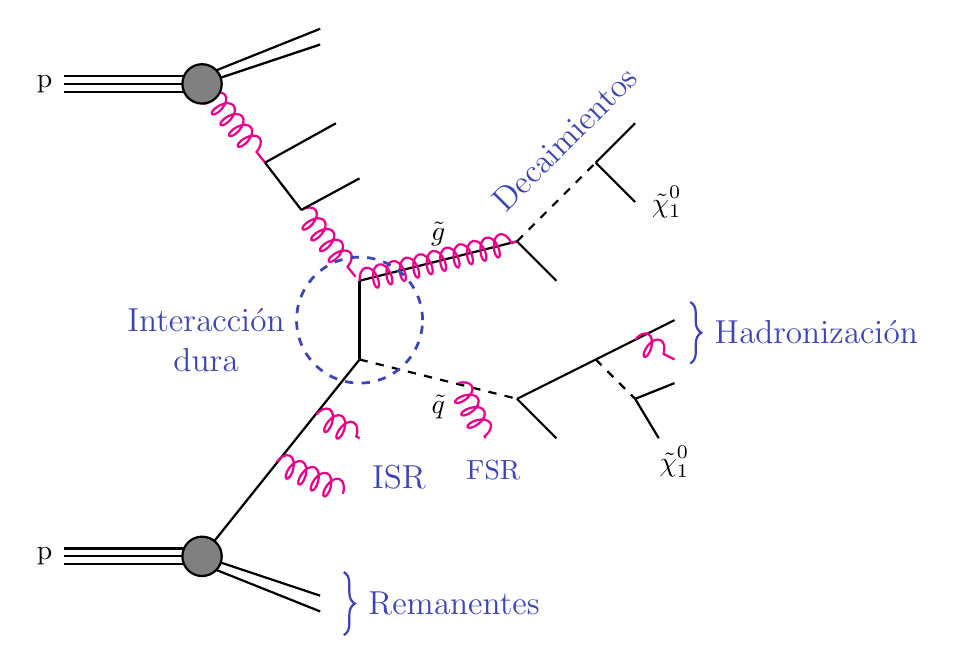
\begin{tikzpicture}

  \tikzset{
    line/.style={line width=0.8},
    dline/.style={dashed,line width=0.9},
  }

  \definecolor{blue1}{HTML}{3C45B7}
  \definecolor{blue2}{HTML}{2C4784}

  %\draw[step=0.5,black!20,thin] (-5,-5) grid (5,5);
  %\draw[step=1,red!30,thin] (-5,-5) grid (5,5);

  \coordinate (p1) at (-2, 3);
  \coordinate (p2) at (-2,-3);
  \coordinate (O) at (2,0);

  \node at (-4, 3) {p};
  \node at (-4,-3) {p};

  \draw[line] (-3.75, 3.1) -- (-2, 3.1);
  \draw[line] (-3.75, 3) -- (p1);
  \draw[line] (-3.75, 2.9) -- (-2, 2.9);

  \draw[line] (-3.75,-2.9) -- (-2, -2.9);
  \draw[line] (-3.75,-3) -- (p2);
  \draw[line] (-3.75,-3.1) -- (-2, -3.1);


  \draw[line] (0,-0.5) -- (0,0.5);
  \draw[line] (p2) -- (0,-0.5);

  \draw[line,gluon] (p1) -- (-1.2, 2);
  \draw[line] (-1.2,2) -- (-0.74,1.4);
  \draw[line,gluon] (-0.74,1.4) -- (-0.05, 0.55);
  \draw[line] (-1.2,2) -- (-0.3, 2.5);
  \draw[line] (-0.74,1.4) -- (0, 1.8);

  \draw[line,dashed] (0,-0.5) -- (2,-1);
  \draw[line,gluon]  (1.25, -0.8) -- (1.6, -1.5);
  \node[line,blue1] at (1.7, -1.9) {FSR};

  \draw[line]         (0, 0.5) -- (2, 1);
  \draw[line,gluon]  (0, 0.5) -- (2, 1);

  \draw[line] (2,-1) -- (2.5,-1.5);
  \draw[line] (2,-1) -- (4, 0);

  \draw[line,dashed] (3, -0.5) -- (3.5,-1);
  \draw[line] (3.5, -1) -- (3.8, -1.50);
  \draw[line] (3.5, -1) -- (4, -0.80);

  \draw[line,dashed] (2, 1) -- (3,2);
  \draw[line] (2, 1) -- (2.5,0.5);

  \draw[line] (-2,3) -- (-0.5,3.5);
  \draw[line] (-2,3.1) -- (-0.5,3.7);

  \draw[line] (-2,  -3) -- (-0.5,-3.5);
  \draw[line] (-2,-3.1) -- (-0.5,-3.7);

  %
  \draw[line,gluon] (-1.05,-1.8) -- (-0.2,-2.2);
  \draw[line,gluon] (-0.55,-1.2) -- (0,-1.5);

  \draw[line] (3,2) -- (3.5,2.5);
  \draw[line] (3,2) -- (3.5,1.5);

  \draw[line,gluon] (3.5,-0.25) -- (4,-0.5);

  \node at (1,1.1) {$\tilde{g}$};
  \node at (1,-1.1) {$\tilde{q}$};
  \node at (4,-1.8) {$\tilde{\chi}^0_1$};
  \node at (3.9,1.5) {$\tilde{\chi}^0_1$};

  \draw[line,dashed,blue1,line width=1] (0,0) circle(0.8);

  \node[blue1] at (-1.95,0) {\large Interacción};
  \node[blue1] at (-1.95,-0.5) {\large dura};

  \node[blue1] at (0.5,-2.0) {\large ISR};
  \node[blue1,rotate=45] at (2.6,2.3) {\large Decaimientos};


  \draw[line,blue1, decorate,decoration={brace,amplitude=4pt}] (4.2,0.23) -- (4.2,-0.55);
  \node[blue1] at (5.8, -0.15) {\large Hadronización};

  \draw[line,blue1, decorate,decoration={brace,amplitude=4pt}] (-0.2,-3.2) -- (-0.2,-4);
  \node[blue1] at (1.2,-3.6) {\large Remanentes};

  \draw[line,fill=gray] (p1) circle(0.25);
  \draw[line,fill=gray] (p2) circle(0.25);

\end{tikzpicture}
}

  \caption{Esquema de las distintos pasos implementados en los generadores de
    eventos Monte Carlo. Adaptado de \cite{Baer:2009tk}.}
  \label{fig:mc_event_generator}

\end{figure}


\subsection{Simulación del detector ATLAS}
\label{sec:sim_atlas}

Para algunos estudios aproximados es posible utilizar directamente las
partículas producidas por los generadores Monte Carlo. Pero en el caso general
es necesario simular el pasaje de estas partículas por el detector.

A fin de poder estudiar la respuesta del detector para un gran número de procesos
físicos y escenarios, se ha implementado una simulación detallada que lleva los
eventos de la generación a un formato que es idéntico a las señales en el
detector verdadero\cite{AtlasSim}. La simulación está integrada al software de
ATLAS (\textsc{Athena}), y utiliza el paquete de simulación
{\geant}4\cite{Geant4}.

La simulación está dividida así en tres etapas: generación del evento y los
decaimientos inmediatos, simulación del detector, y digitalización de
los depósitos de energía en las regiones sensibles del detector en los voltajes
y corrientes que se encuentran a la salida del detector. Luego, la salida de
estos procesos de simulación sirve como entrada a los algoritmos de
\emph{trigger} y reconstrucción de ATLAS, que son idénticos a los que se utilizan en
los datos reales.

Existe también una simulación rápida del detector que es utilizada en los casos
donde no es necesaria un simulación tan minuciosa de las lluvias
electromagnéticas en los calorímetros. Casi 80\% del tiempo de simulación se
debe a la simulación de partículas atravesando el calorímetro, y cerca del 75\%
se emplea en la simulación de las partículas electromagnéticas. En la simulación
rápida \textsc{Atlfast}\cite{Richter-Was:683751}, se remueven estas partículas
electromagnéticas de baja energía y se las reemplaza con lluvias
electromagnéticas pre-simuladas. De esta forma se reduce el consumo de CPU
notablemente considerando las características de la física en cuestión.

En las simulaciones Monte Carlo, el \emph{pile-up in-time} es incorporado
superponiendo las señales de los procesos físicos de interés con señales
correspondientes a un dado número de colisiones adicionales independientes de
\emph{minimum-bias}.
Cada evento en una muestra Monte Carlo es producido bajo ciertas condiciones
particulares del detector, y bajo un valor particular de \emph{pile-up}. Existen
algunas diferencias en el perfil del \emph{pile-up} de los datos reales y las muestras
MC, en particular debido a que las muestras MC son simuladas previo a la toma de
datos con el \emph{pile-up} previsto que no es exactamente igual al real. Para
solucionar esto, se aplica un repesado evento a evento a las muestras MC de
manera de modelar las condiciones reales de la muestra de datos bajo estudio.

\section{Simulación de la señal de SUSY}\label{sec:sig_samples}

Como se ha mencionado en el \cref{cap:susy}, debido al gran número de parámetros
libres en los modelos de SUSY, las búsquedas de supersimetría en ATLAS están
impulsadas por la fenomenología de los estados finales. El análisis realizado
para esta tesis está motivado por estados finales con fotones energéticos,
provenientes del decaimiento de un neutralino NLSP en el contexto de modelos
GGM.

En los modelos GGM el decaimiento de los estados supersimétricos producidos en
las colisiones del LHC va a proceder por medio de decaimientos en cascada hasta
el neutralino NLSP que decaerá a un gravitino y una partícula del SM, que
dependerá de la naturaleza de la NSLP. Distintas posibilidades para la
naturaleza de la NLSP pueden ser consideradas, las cuales dan lugar a estados
finales distintos y complementarios entre si, para cubrir las distintas regiones
del espacio de fase de los modelos GGM. Dentro de ATLAS se exploraron cuatro
estados finales diferentes: dos fotones, un fotón y un leptón, un fotón y
{\bjets}, y un fotón y jets, todos con energía faltante, correspondiente a los
gravitinos LSP.

En particular en esta tesis se focalizó en el análisis de un estado final que
consiste en un único fotón, jets y energía faltante.
La selección de eventos que se describe en el \cref{cap:seleccion} fue diseñada para
maximizar la sensibilidad a pequeñas señales con esta topología general.
Cualquier imposición de cortes muy dependientes del modelo fueron evitadas,
tratando de mantener el análisis lo más independiente del modelo como fuera
posible. Sin embargo, una interpretación en el marco de un modelo especifico es
inevitable. Con tal motivo se simuló un conjunto de puntos de señal con
distintos valores de los parámetros para cubrir la región del espacio de
parámetros donde pueda manifestarse dicha señal.

%% Se simularon puntos de senal para la produccion de gluinosLos resultados se interpretaron
%% son interpretados en el contexto de GGM que
%% incluyen la produccion de supercompaneras de particulas del SM que se acoplan
%% fuertemente comot ambien de que poseen solo carga electrodebil.

Se utilizó un espectro simplificado en el cual, básicamente, el espacio de
parámetros consiste en la escala de producción (por simplicidad, la masa del
gluino) y la masa de la NLSP. Todos los demás estados fueron desacoplados ya que
no juegan un rol importante en la producción o en el estado final de interés.
Esta aproximación es similar a los denominados <<modelos simplificados>>
utilizados en otras búsquedas.
La masa del gluino es el único parámetro libre de las partículas de color para
poder determinar un límite conservativo en la masa del mismo. Todos los
parámetros de masa \emph{soft} de los \emph{squarks} se fijan en 2.5 \tev.

Para maximizar la probabilidad de tener un único fotón en el estado final, es
necesario que $\mathrm{BR}(\ninoone \to \gam\,\gravino) \sim 50\%$. Esto resulta
cuando el neutralino más liviano es una mezcla bino-higgsino. Además, el valor
de $\mu$ debe ser positivo para suprimir el decaimiento a Higgs, que llevará a
un estado final ya cubierto por otro análisis de ATLAS. Para lograr la BR
deseada se variaron los parámetros de masa de bino ($M_1$) y higgsinos ($\mu$)
para las diferentes masas del {\ninoone}, de tal forma que los BR del {\ninoone}
sean aproximadamente constantes:

\begin{align}
  &\mathrm{BR}(\ninoone \to \gam\, \gravino) \approx 50\% \label{eq:n1_gam}\\
  &\mathrm{BR}(\ninoone \to Z\, \gravino) \approx 49\%    \label{eq:n1_z} \\
  &\mathrm{BR}(\ninoone \to h\, \gravino) \approx 1\%     \label{eq:n1_h}
\end{align}


Los demás parámetros del modelo se fijan en $M_2=2.5\tev$, $\tan\beta=1.5$ y
$c\tau_{\mathrm{NLSP}} < 0.1$ mm. Este último asegura que el neutralino decaiga
rápidamente dentro del detector y se logra haciendo al gravitino lo
suficientemente liviano ($m_{\tilde{G}}=10^{-9} \gev$). Todos los términos
tri-lineares son fijados a cero y las masas de los sleptones a $2.5 \tev$.
Las masas del higgs liviano ($h$) y el pseudoescalar ($A$) se fijan a
$m_{h} = 126 \gev$ y $m_{A} = 2 \tev$.
La masa del $h$ se considera a partir del valor
medido de la masa del Higgs observado en el a\~no 2012.
En modelos GGM de SUSY existen distintos
mecanismos\cite{Craig:2011yk,Auzzi:2011eu,Csaki:2012fh,Larsen:2012rq,Craig:2012hc}
para generar una masa del bosón de Higgs tan alta como este valor observado, sin
cambiar la fenomenología de los modelos considerados. No se observó un efecto
significativo en el espectro de masas variando el valor de la masa de Higgs en un
rango de $\pm 10 \gev$.
%% Tambien se estudio el efecto de variar el valor
%% de $\tan\beta$\note{Hacer comentario de $\tan\beta$}

A partir de estos estudios se procedió a simular un conjunto de puntos de señal
(\emph{grid}) en el plano ($m_{\gluino}$, $m_{\ninoone}$), variando los parámetros
$M_3$ y $\mu$. El parámetro $M_1$ se ajustó, dependiendo del $\mu$ de forma de
obtener las BR descriptas anteriormente. La \emph{grid} cubre el espacio $150\gev <
m_{\ninoone} < 1250 \gev$ y $800\gev < m_{\gluino} < 1300 \gev$, con
$m_{\ninoone} < m_{\gluino}$ (ver \cref{fig:gridpoints}).


\begin{figure}[!htb]
  \centering
  \includegraphics[width=0.6\textwidth]{figures/run1_grid}
  \caption{Conjunto de puntos (\emph{grid}) de señal simulada para el presente
    análisis. Los cuadrados azules representan los distintos puntos de señal
    generados con distintos valores de $m_{\gluino}$ y $m_{\ninoone}$. También
    puede verse la relación con las masas $m_{\gluino}$ y $m_{\ninoone}$.}
  \label{fig:gridpoints}
\end{figure}


El espectro completo de masas y los correspondientes decaimientos fueron
calculados a partir de estos parámetros utilizando {\suspect}
(v2.41)\cite{Djouadi2007426}, {\sdecay} (v1.3b)\cite{Muhlleitner:2004mka} y
{\hdecay} (v3.4)\cite{Djouadi:1997yw}, que forman parte del paquete {\susyhit}
(v1.3)\cite{Djouadi:2006bz}. Algunos ejemplos del espectro de masas pueden verse
en la \cref{fig:mass_spectra}, para algunos puntos de la \emph{grid}, (885, 146) y (1463, 1053).

\begin{figure}[!htb]
  \centering

  \resizebox{0.49\textwidth}{!}{\begin{tikzpicture}[scale=0.6]
  % y-scalefactor (GeV -> coords) = 5.133333e-03

  %% Frame
  \draw (-2.000000,0.000000) rectangle (19.000000,15.400000);

  %% y-ticks
  \draw (-2.000000,0.000000) node[left] {\large 0};

  \draw (-2.000000,2.053333) node[left] {\large 400};
  \draw (-1.700000,2.053333) -- (-2.000000,2.053333);
  \draw (18.700000,2.053333) -- (19.000000,2.053333);

  \draw (-2.000000,4.106667) node[left] {\large 800};
  \draw (-1.700000,4.106667) -- (-2.000000,4.106667);
  \draw (18.700000,4.106667) -- (19.000000,4.106667);

  \draw (-2.000000,6.160000) node[left] {\large 1200};
  \draw (-1.700000,6.160000) -- (-2.000000,6.160000);
  \draw (18.700000,6.160000) -- (19.000000,6.160000);

  \draw (-2.000000,8.213333) node[left] {\large 1600};
  \draw (-1.700000,8.213333) -- (-2.000000,8.213333);
  \draw (18.700000,8.213333) -- (19.000000,8.213333);

  \draw (-2.000000,10.266667) node[left] {\large 2000};
  \draw (-1.700000,10.266667) -- (-2.000000,10.266667);
  \draw (18.700000,10.266667) -- (19.000000,10.266667);

  \draw (-2.000000,12.320000) node[left] {\large 2400};
  \draw (-1.700000,12.320000) -- (-2.000000,12.320000);
  \draw (18.700000,12.320000) -- (19.000000,12.320000);

  \draw (-2.000000,14.373333) node[left] {\large 2800};
  \draw (-1.700000,14.373333) -- (-2.000000,14.373333);
  \draw (18.700000,14.373333) -- (19.000000,14.373333);

  \draw (-4,15.400000) node[left,rotate=90] {\large Mass [GeV]};

  %% Particle lines
  % pid25
  \draw[color=blue,thick] (-0.200000,0.646800) -- (1.800000,0.646800);
  % pid35
  \draw[color=blue,thick] (-0.200000,10.287452) -- (1.800000,10.287452);
  % pid36
  \draw[color=blue,thick] (-0.200000,10.266667) -- (1.800000,10.266667);
  % pid37
  \draw[color=red,thick] (0.200000,10.277936) -- (2.200000,10.277936);
  % pid1000001
  \draw[color=blue,thick] (14.900000,12.801359) -- (16.900000,12.801359);
  % pid1000005
  \draw[color=black!50!blue!30!green,thick] (15.200000,12.799941) -- (17.200000,12.799941);
  % pid1000006
  \draw[color=red,thick] (15.200000,12.969641) -- (17.200000,12.969641);
  % pid1000011
  \draw[color=blue,thick] (4.800000,12.834192) -- (6.800000,12.834192);
  % pid1000012
  \draw[color=blue,thick] (4.800000,12.831692) -- (6.800000,12.831692);
  % pid1000015
  \draw[color=red,thick] (5.200000,12.833745) -- (7.200000,12.833745);
  % pid1000016
  \draw[color=red,thick] (5.200000,12.831692) -- (7.200000,12.831692);
  % pid1000021
  \draw[color=black!50!blue!30!green,thick] (14.700000,4.782759) -- (16.700000,4.782759);
  % pid1000022
  \draw[color=blue,thick] (9.800000,0.754562) -- (11.800000,0.754562);
  % pid1000023
  \draw[color=blue,thick] (9.800000,0.827094) -- (11.800000,0.827094);
  % pid1000024
  \draw[color=red,thick] (10.200000,0.813201) -- (12.200000,0.813201);
  % pid1000025
  \draw[color=blue,thick] (9.800000,1.673399) -- (11.800000,1.673399);
  % pid1000035
  \draw[color=blue,thick] (9.800000,13.116866) -- (11.800000,13.116866);
  % pid1000037
  \draw[color=red,thick] (10.200000,13.116862) -- (12.200000,13.116862);
  % pid1000039
  \draw[color=black!50!blue!30!green,thick] (10.150000,0.000000) -- (12.150000,0.000000);
  % pid2000001
  \draw[color=blue,thick] (14.900000,12.800219) -- (16.900000,12.800219);
  % pid2000005
  \draw[color=black!50!blue!30!green,thick] (15.200000,12.801653) -- (17.200000,12.801653);
  % pid2000006
  \draw[color=red,thick] (15.200000,13.792202) -- (17.200000,13.792202);
  % pid2000011
  \draw[color=blue,thick] (4.800000,12.834116) -- (6.800000,12.834116);
  % pid2000015
  \draw[color=red,thick] (5.200000,12.834569) -- (7.200000,12.834569);

  %% Particle labels
  \draw (-0.4,0.646800)  node[left]  {\large $h^0$};
  \draw (-0.4,9.963600)  node[left]  {\large $A^0$};
  \draw (-0.4,10.590518) node[left]  {\large $H^0$};
  \draw (2.4,10.277936)  node[right] {\large $H^\pm$};
  \draw (14.7,12.387330) node[left]  {\large $\tilde{q}_\text{R}$};
  \draw (14.7,13.114248) node[left]  {\large $\tilde{q}_\text{L}$};
  \draw (17.4,11.9) node[right] {\large $\tilde{b}_1$};
  \draw (17.4,12.801653) node[right] {\large $\tilde{b}_2$};
  \draw (17.4,13.511709) node[right] {\large $\tilde{t}_1$};
  \draw (4.6,12.006024)  node[left]  {\large $\tilde{\nu}_\text{L}$};
  \draw (4.6,12.834116)  node[left]  {\large $\tilde{\ell}_\text{R}$};
  \draw (4.6,13.659860)  node[left]  {\large $\tilde{\ell}_\text{L}$};
  \draw (7.4,12.206212)  node[right] {\large $\tilde{\nu}_\tau$};
  \draw (7.4,12.833745)  node[right] {\large $\tilde{\tau}_1$};
  \draw (7.4,13.460049)  node[right] {\large $\tilde{\tau}_2$};
  \draw (14.500000,4.782759)  node[left]  {\large $\tilde{g}$};
  \draw (9.600000,0.407369)   node[left]  {\large $\tilde{\chi}_1^0$};
  \draw (9.600000,1.304287)   node[left]  {\large $\tilde{\chi}_2^0$};
  \draw (12.350000,0.32)  node[right] {\large $\tilde{G}$};
  \draw (12.4,1.2)  node[right] {\large $\tilde{\chi}_1^\pm$};
  \draw (9.6,2.27)   node[left]  {\large $\tilde{\chi}_3^0$};
  \draw (9.6,13.116866)  node[left]  {\large $\tilde{\chi}_4^0$};
  \draw (12.4,13.116862) node[right] {\large $\tilde{\chi}_2^\pm$};
  \draw (17.4,14.292202) node[right] {\large $\tilde{t}_2$};

\end{tikzpicture}
}
  \resizebox{0.49\textwidth}{!}{\begin{tikzpicture}[scale=0.6]
  % y-scalefactor (GeV -> coords) = 5.310345e-03

  %% Frame
  \draw (-2.000000,0.000000) rectangle (19.000000,15.400000);
  %% y-ticks
  \draw (-2.000000,0.000000) node[left] {\large 0};
  \draw (-2.000000,2.124138) node[left] {\large 400};
  \draw (-1.700000,2.124138) -- (-2.000000,2.124138);
  \draw (18.700000,2.124138) -- (19.000000,2.124138);

  \draw (-2.000000,4.248276) node[left] {\large 800};
  \draw (-1.700000,4.248276) -- (-2.000000,4.248276);
  \draw (18.700000,4.248276) -- (19.000000,4.248276);

  \draw (-2.000000,6.372414) node[left] {\large 1200};
  \draw (-1.700000,6.372414) -- (-2.000000,6.372414);
  \draw (18.700000,6.372414) -- (19.000000,6.372414);

  \draw (-2.000000,8.496552) node[left] {\large 1600};
  \draw (-1.700000,8.496552) -- (-2.000000,8.496552);
  \draw (18.700000,8.496552) -- (19.000000,8.496552);

  \draw (-2.000000,10.620690) node[left] {\large 2000};
  \draw (-1.700000,10.620690) -- (-2.000000,10.620690);
  \draw (18.700000,10.620690) -- (19.000000,10.620690);

  \draw (-2.000000,12.744828) node[left] {\large 2400};
  \draw (-1.700000,12.744828) -- (-2.000000,12.744828);
  \draw (18.700000,12.744828) -- (19.000000,12.744828);

  \draw (-2.000000,14.868966) node[left] {\large 2800};
  \draw (-1.700000,14.868966) -- (-2.000000,14.868966);
  \draw (18.700000,14.868966) -- (19.000000,14.868966);

  \draw (-4,15.400000) node[left,rotate=90] {\large Mass [GeV]};

  %% Particle lines
  % pid25
  \draw[color=blue,thick] (-0.200000,0.669103) -- (1.800000,0.669103);
  % pid35
  \draw[color=blue,thick] (-0.200000,10.642196) -- (1.800000,10.642196);
  % pid36
  \draw[color=blue,thick] (-0.200000,10.620690) -- (1.800000,10.620690);
  % pid37
  \draw[color=red,thick] (0.200000,10.629204) -- (2.200000,10.629204);
  % pid1000001
  \draw[color=blue,thick] (14.900000,12.935241) -- (16.900000,12.935241);
  % pid1000005
  \draw[color=black!50!blue!30!green,thick] (15.200000,12.929948) -- (17.200000,12.929948);
  % pid1000006
  \draw[color=red,thick] (15.200000,13.054650) -- (17.200000,13.054650);
  % pid1000011
  \draw[color=blue,thick] (4.800000,13.276745) -- (6.800000,13.276745);
  % pid1000012
  \draw[color=blue,thick] (4.800000,13.274169) -- (6.800000,13.274169);
  % pid1000015
  \draw[color=red,thick] (5.200000,13.273736) -- (7.200000,13.273736);
  % pid1000016
  \draw[color=red,thick] (5.200000,13.274169) -- (7.200000,13.274169);
  % pid1000021
  \draw[color=black!50!blue!30!green,thick] (14.700000,7.771358) -- (16.700000,7.771358);
  % pid1000022
  \draw[color=blue,thick] (9.800000,5.591817) -- (11.800000,5.591817);
  % pid1000023
  \draw[color=blue,thick] (9.800000,5.877497) -- (11.800000,5.877497);
  % pid1000024
  \draw[color=red,thick] (10.200000,5.855077) -- (12.200000,5.855077);
  % pid1000025
  \draw[color=blue,thick] (9.800000,6.058680) -- (11.800000,6.058680);
  % pid1000035
  \draw[color=blue,thick] (9.800000,13.566086) -- (11.800000,13.566086);
  % pid1000037
  \draw[color=red,thick] (10.200000,13.566067) -- (12.200000,13.566067);
  % pid1000039
  \draw[color=black!50!blue!30!green,thick] (10.150000,0.000000) -- (12.150000,0.000000);
  % pid2000001
  \draw[color=blue,thick] (14.900000,12.934054) -- (16.900000,12.934054);
  % pid2000005
  \draw[color=black!50!blue!30!green,thick] (15.200000,12.939362) -- (17.200000,12.939362);
  % pid2000006
  \draw[color=red,thick] (15.200000,13.907036) -- (17.200000,13.907036);
  % pid2000011
  \draw[color=blue,thick] (4.800000,13.276672) -- (6.800000,13.276672);
  % pid2000015
  \draw[color=red,thick] (5.200000,13.279687) -- (7.200000,13.279687);

  %% Particle labels
  \draw (-0.400000,0.669103) node[left] {\large $h^0$};
  \draw (-0.400000,10.315374) node[left] {\large $A^0$};
  \draw (-0.400000,10.947512) node[left] {\large $H^0$};
  \draw (2.400000,10.629204) node[right] {\large $H^\pm$};
  \draw (14.700000,12.518579) node[left] {\large $\tilde{q}_\text{R}$};
  \draw (14.700000,13.250717) node[left] {\large $\tilde{q}_\text{L}$};
  \draw (17.400000,12.160161) node[right] {\large $\tilde{b}_1$};
  \draw (17.400000,12.939362) node[right] {\large $\tilde{b}_2$};
  \draw (17.400000,13.624437) node[right] {\large $\tilde{t}_1$};
  \draw (4.600000,12.45) node[left] {\large $\tilde{\nu}_\text{L}$};
  \draw (4.600000,13.276672) node[left] {\large $\tilde{\ell}_\text{R}$};
  \draw (4.600000,13.907595) node[left] {\large $\tilde{\ell}_\text{L}$};
  \draw (7.400000,12.644574) node[right] {\large $\tilde{\tau}_1$};
  \draw (7.400000,13.274169) node[right] {\large $\tilde{\nu}_\tau$};
  \draw (7.400000,13.908850) node[right] {\large $\tilde{\tau}_2$};
  \draw (14.500000,7.771358) node[left] {\large $\tilde{g}$};
  \draw (9.600000,4.9) node[left] {\large $\tilde{\chi}_1^0$};
  \draw (9.600000,5.877497) node[left] {\large $\tilde{\chi}_2^0$};
  \draw (9.600000,6.85) node[left] {\large $\tilde{\chi}_3^0$};
  \draw (12.400000,5.855077) node[right] {\large $\tilde{\chi}_1^\pm$};
  \draw (9.600000,13.566086) node[left] {\large $\tilde{\chi}_4^0$};
  \draw (12.400000,13.566067) node[right] {\large $\tilde{\chi}_2^\pm$};
  \draw (12.350000,0.479283) node[right] {\large $\tilde{G}$};
  \draw (17.400000,14.207036) node[right] {\large $\tilde{t}_2$};
\end{tikzpicture}
}

   %% \includegraphics[width=0.49\textwidth]{figures/masses_GGM_M3_mu_800_150}
   %% %%\includegraphics[width=0.45\textwidth]{figures/masses_GGM_M3_mu_1000_750}
   %% \includegraphics[width=0.49\textwidth]{figures/masses_GGM_M3_mu_1450_1050}

   \caption{Espectro de masas de las partículas supersimétricas para dos puntos de la \emph{grid} de señal.
     En la izquierda para (885,146) y en la derecha (1463, 1053), en el plano \mgmn.}
   \label{fig:mass_spectra}
\end{figure}

Para cada uno de los 124 puntos de señal que constituyen la \emph{grid} se generaron
5000 eventos, utilizando {\herwigpp} v2.5.2\cite{Bahr:2008pv} y el conjunto de
PDFs CTEQ6L1\cite{Nadolsky:2008zw}. Se aplicó un filtro a nivel generador, que
requería la presencia de un fotón con un {\pt} de al menos 100 \gev, para
optimizar la generación, especialmente en los puntos donde el
neutralino tiene menor masa. La eficiencia del filtro para todas las muestras
simuladas puede verse en la \cref{tab:signal_filter_eff}. La simulación del
detector ATLAS se realizó con la simulación rápida
\textsc{ATLFAST-II}\cite{Richter-Was:683751}.


\begin{table}[!htb]
  \centering
  \caption{Relación entre los parámetros libres del modelo $M_3$ y $\mu$ con las
    masas $m_{\gluino}$ (izquierda) y $m_{\ninoone}$ (derecha), respectivamente.
    En la tabla de la derecha, para cada valor de $\mu$ también se puede
    observar el valor de $M_1$ utilizado para obtener los BR de decaimiento del
    {\ninoone} deseados.}
  \label{tab:signal_pars}

  \begin{minipage}[!t]{0.5\textwidth}
    \centering
    \begin{tabular}{cc}
      \hline
      $M_3$ [\gev]& $m_{\gluino}$ [\gev] \\
      \hline
      800  & 885.5 \\
      850  & 931.7 \\
      900  & 977.6 \\
      950  & 1023.1 \\
      1000 & 1068.3  \\
      1050 & 1113.3  \\
      1100 & 1157.9  \\
      1150 & 1202.3  \\
      1200 & 1246.4  \\
      1250 & 1290.3  \\
      1300 & 1333.9  \\
      1350 & 1377.3  \\
      1400 & 1420.5  \\
      1450 & 1463.4  \\
      \hline
    \end{tabular}
    \vspace{5cm}
  \end{minipage}%
  \begin{minipage}[t]{0.5\textwidth}
    \begin{tabular}{ccc}
      \hline
      $\mu$ [\gev] & $M_1$ [\gev] & $m_{\ninoone}$ [\gev] \\
      \hline
      150  &  300  & 147.0 \\
      175  &  270  & 168.3 \\
      200  &  267  & 190.3 \\
      250  &  288  & 235.8 \\
      350  &  365  & 332.4 \\
      450  &  456  & 433.2 \\
      550  &  551  & 535.6 \\
      650  &  647  & 638.3 \\
      750  &  745  & 742.0 \\
      838  &  837  & 836.4 \\
      850  &  845  & 846.7 \\
      883  &  882  & 883.7 \\
      928  &  926  & 930.2 \\
      950  &  942  & 949.6 \\
      973  &  970  & 976.6  \\
      1017 &  1015 & 1023.4 \\
      1050 &  1040 & 1053.0 \\
      1062 &  1058 & 1068.9 \\
      1106 &  1102 & 1114.8 \\
      1149 &  1145 & 1160.0 \\
      1150 &  1140 & 1157.5 \\
      1250 &  1238 & 1260.6 \\
      \hline
    \end{tabular}

  \end{minipage}

\end{table}


\begin{table}[ht]
  \centering

  \footnotesize
  \caption{Eficiencia del filtro a nivel generador [\%]
    para los puntos de señal simulados.}

  \scalebox{0.8}{
  \begin{tabular}{c|ccccccccccccccccc}
    \hline
     &   \multicolumn{14}{c}{ $M_3$ [\gev] } \\
    $\mu$ [\gev] &  800 & 850 & 900 & 950 & 1000 & 1050 & 1100 &1150 & 1200  & 1250 & 1300 & 1350 & 1400 & 1450 \\
    \hline
    150  &   39.54 &   39.8 &  41.9    &   42.6   &   43.0   &   44.2   &   45.5    &   46.3    &    47.1  &   48.3  &   49.1 &      &      &       \\
    175  &   44.55 &   44.6 &  46.5    &   47.5   &   47.8   &   48.9   &   50.3    &   51.4    &    51.5  &   52.4  &   53.3 &      &      &       \\
    200  &   47.66 &   48.4 &  50.1    &   50.6   &   52.0   &   52.8   &   53.8    &   55.0    &    55.0  &   56.2  &   56.0 &      &      &       \\
    250  &   55.09 &   56.0 &  56.1    &   57.1   &   56.7   &   58.0   &   58.9    &   59.5    &    60.5  &   60.7  &   61.2 & 62.1 & 62.2 &  63.9 \\
    350  &   65.82 &   66.1 &  64.6    &   65.8   &   66.4   &   66.7   &   66.5    &   67.7    &    67.4  &   67.6  &   67.8 & 68.0 & 69.2 &  68.4 \\
    450  &   71.29 &   71.4 &  71.4    &   71.8   &   72.1   &   72.5   &   72.0    &   72.6    &    72.1  &   72.5  &   73.4 & 72.9 & 72.2 &  73.4 \\
    550  &   73.08 &   72.5 &  73.3    &   73.7   &   74.6   &   74.3   &   75.0    &   74.8    &    74.2  &   74.7  &   75.6 & 75.7 & 74.9 &  75.3 \\
    650  &   69.78 &   72.0 &  73.2    &   74.1   &   75.6   &   76.2   &   75.9    &   75.8    &    77.0  &   77.0  &   76.2 & 76.7 & 77.1 &  76.6 \\
    750  &   47.69 &   60.2 &  66.9    &   70.4   &   73.4   &   74.0   &   75.9    &   76.5    &    77.1  &   77.3  &   76.3 & 77.9 & 77.2 &  77.0 \\
    838  &    9.0  &        &          &          &          &          &           &           &          &         &        &      &      &       \\
    883  &         &   9.1  &          &          &          &          &           &           &          &         &        &      &      &       \\
    850  &         &        &  34.2    &   50.7   &   60.1   &   66.4   &   70.4    &   73.5    &    73.6  &   75.4  &   76.6 & 77.1 & 78.2 &  76.8 \\
    928  &         &        &   9.4    &          &          &          &           &           &          &         &        &      &      &       \\
    950  &         &        &          &          &   25.4   &   41.4   &   54.0    &   62.2    &    66.8  &   70.9  &   75.2 & 75.9 & 78.1 &  77.2 \\
    973  &         &        &          &   10.0   &          &          &           &           &          &         &        &      &      &       \\
    1017 &         &        &          &          &   10.3   &          &           &           &          &         &        &      &      &       \\
    1050 &         &        &          &          &          &          &   19.2    &   31.6    &    45.2  &   56.8  &   62.7 & 68.9 & 73.1 &  75.6 \\
    1062 &         &        &          &          &          &   11.1   &           &           &          &         &        &      &      &       \\
    1106 &         &        &          &          &          &          &   11.7    &           &          &         &        &      &      &       \\
    1149 &         &        &          &          &          &          &           &   12.6    &          &         &        &      &      &       \\
    1150 &         &        &          &          &          &          &           &           &    16.1  &   24.9  &   36.9 & 49.0 &      &       \\
    1250 &         &        &          &          &          &          &           &           &          &         &   16.1 &      &      &       \\
    \hline
  \end{tabular}
  }
  \label{tab:signal_filter_eff}
\end{table}



\subsection{Estudios a nivel generador}
\label{sec:susy_studies}

Se realizaron algunos estudios para entender mejor el estado final y poder
identificar las distintas regiones en el espacio de fase, lo cual facilitaría el
proceso de optimización de las posibles regiones de se\~nal. En la
\cref{fig:signal_br_gl} se presentan los distintos BR de los gluinos para todos
los puntos de la \emph{grid}. Resulta evidente que la cadena de decaimiento dominante
varía en las distintas regiones de la \emph{grid}, dependiendo de la masa del gluino y
el neutralino. Se puede ver que el decaimiento dominante es a través de
charginos, pero a medida que la masa del gluino y el neutralino se acercan,
empieza a resultar más importante el decaimiento directo al neutralino más
liviano, mientras que en los puntos más cercanos a la diagonal, el decaimiento
estará dominado por $\gluino\to g\gravino$ el cual no corresponde al estado
final deseado. Los diagramas de los distintos decaimientos posibles se encuentran
en la \cref{fig:signal_diagrams}, de los cuales se pueden extraer varias
conclusiones: en el caso de las cadenas largas a través de charginos, el estado
final tendrá una mayor cantidad de jets. Si el decaimiento es directamente al
{\ninoone} la multiplicidad de jets será menor y la energía del fotón será mayor
al igual que la energía faltante.


\begin{figure}[!htb]
  \centering

  \includegraphics[width=0.5\textwidth]{figures/br_gl_X}

  \caption{Tasas de decaimiento (BR) de los gluinos para los distintos puntos de la \emph{grid} en
    el plano \mgmn. Para cada punto de señal, la fracción del rectángulo de cada color representa
    el BR a cada uno de los posibles estados finales.}
  \label{fig:signal_br_gl}
\end{figure}


\begin{figure}[!htb]
  \centering

  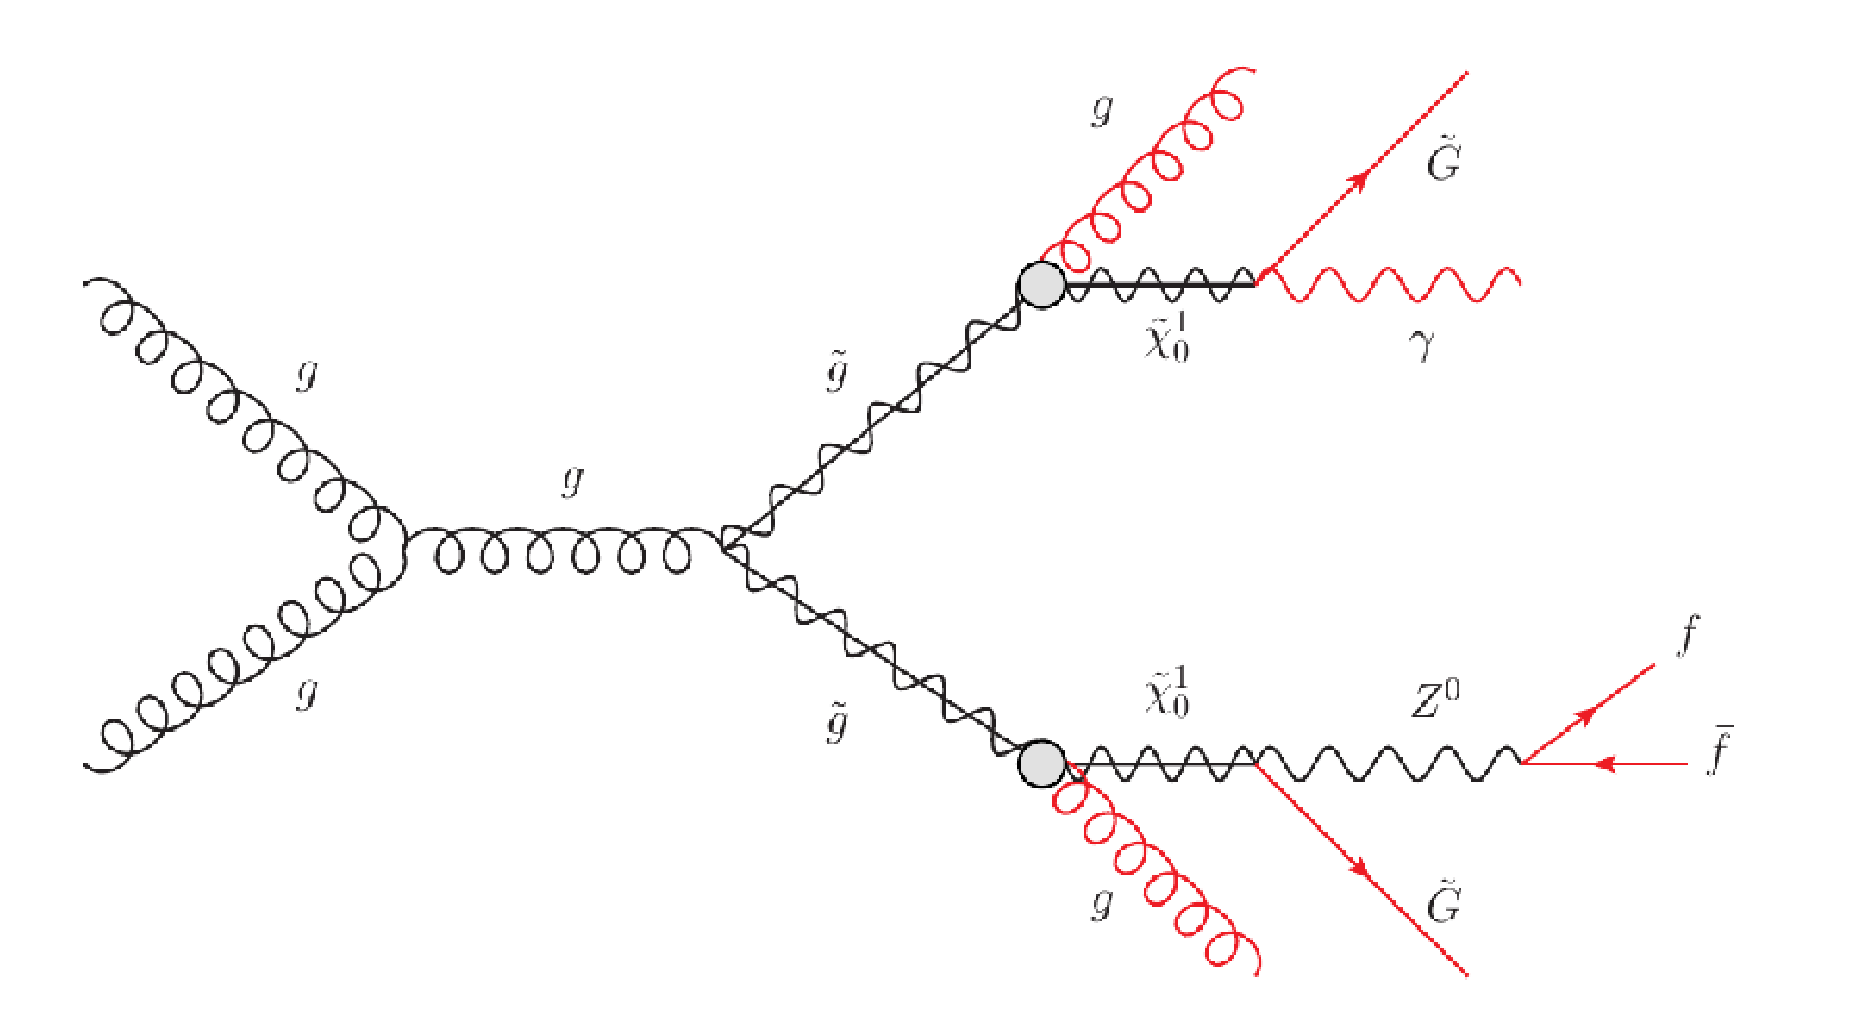
\includegraphics[width=0.49\textwidth]{diagram_a}
  \includegraphics[width=0.49\textwidth]{diagram_b}

  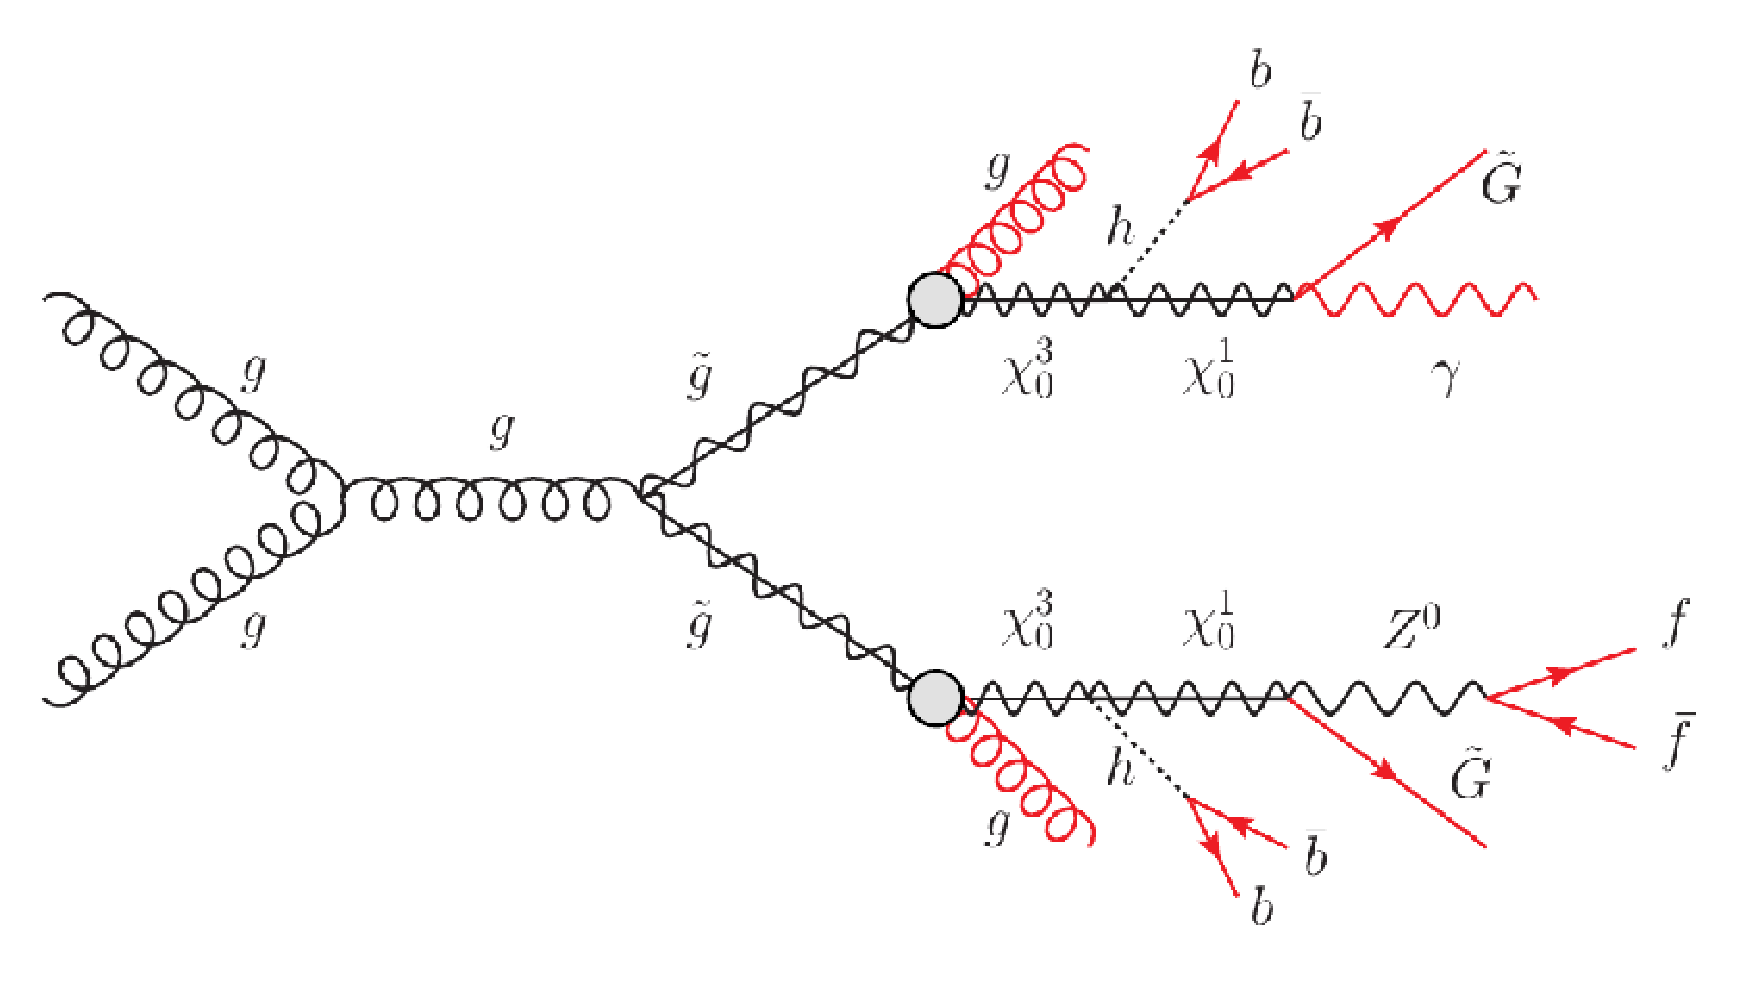
\includegraphics[width=0.49\textwidth]{diagram_c}
  \includegraphics[width=0.49\textwidth]{diagram_d}

  \caption{Diagramas de Feynman para la producción de gluinos y el subsiguiente
    decaimiento de los mismos hasta el estado final. Los distintos diagramas ilustran
    las posibles cadenas de decaimiento.}
  \label{fig:signal_diagrams}

\end{figure}


En la \cref{fig:signal_br_n1} se presentan las BR de decaimiento del neutralino
más liviano (\ninoone), compatibles con las esperadas a partir del modelo que se
utilizará para el presente análisis (\cref{eq:n1_gam,eq:n1_z,eq:n1_h}). Estos
valores varían en menos del 1\% en los distintos puntos de la \emph{grid}, salvo para
neutralinos livianos ($<200\gev$) donde la producción de Higgs es altamente
suprimida, mientras aumenta el decaimiento a $Z$, y $\mathrm{BR}(\ninoone \to
\gam \gravino)$ empieza a caer llegando al 40\%.

\begin{figure}[!htb]
  \centering

  \includegraphics[width=0.5\textwidth]{figures/br_n1_X}

  \caption{Tasas de decaimiento (BR) de los neutralinos LSP en $\gamma\gravino$, $\gamma Z$ y
    $\gamma h$ para los distintos puntos de la \emph{grid} en el plano \mgmn. Para cada punto de señal,
    la fracción del rectángulo de cada color representa el BR a cada uno de los posibles estados finales.}
  \label{fig:signal_br_n1}
\end{figure}



\subsection{Sección eficaz de producción}
\label{sec:xs_calc}

En el caso de procesos de producción de pares de gluinos o \emph{squarks}, de los cuales
existe el cálculo a NLL, la sección eficaz se toma a NLO en la constante de acoplamiento
fuerte, y se incluye la suma de la emisión de gluones \emph{soft} con precisión NLL,
realizada utilizando {\nllfast}\cite{Kramer:2012bx,Beenakker:1996ch,Kulesza:2008jb,Kulesza:2009kq,Beenakker:2009ha,Beenakker:2011fu}.

En el caso de la producción de otro tipo de procesos, como la producción electrodébil de
partículas supersimétricas, se utilizan
las secciones eficaces calculadas a NLO usando {\prospino} \cite{Beenakker:1996ed}.


\newcommand{\pdfcteqpm}{\ensuremath{\Delta\mathrm{PDF}^{\pm}(\mathrm{CTEQ})}}
\newcommand{\scacteqpm}{\ensuremath{\Delta\mathrm{SCA}^{\pm}(\mathrm{CTEQ})}}

\newcommand{\pdfmstwpm}{\ensuremath{\Delta\mathrm{PDF}^{\pm}(\mathrm{MSTW})}}
\newcommand{\scamstwpm}{\ensuremath{\Delta\mathrm{SCA}^{\pm}(\mathrm{MSTW})}}

\newcommand{\alphap}{\ensuremath{\alpha_s_+}}
\newcommand{\alpham}{\ensuremath{\alpha_s^-}}
\newcommand{\alphapm}{\ensuremath{\alpha_s^{\pm}}}

Las incertezas debidas a la elección de la escala de renormalización y
factorización como también aquellas asociadas a la PDF, son obtenidas utilizando {\nllfast} o
calculadas con {\prospino}. A fin de combinar todas estas predicciones y obtener
una incerteza total, se siguen las recomendaciones PDF4LHC\cite{Botje:2011sn}.
Para esto se define la envolvente de las predicciones a la sección eficaz usando
el intervalo a 68\% CL del conjunto de PDFs CTEQ (incluyendo la incerteza en
$\alpha_s$) y MSTW, junto con las variaciones de las escalas. La sección eficaz
nominal se obtiene usando el punto medio de la envolvente y la incerteza como la
mitad del ancho de la misma. Matemáticamente si {\pdfcteqpm} y {\scacteqpm} son
las variaciones en $\pm 1\sigma$ de las PDF CTEQ,  {\pdfmstwpm} y {\scamstwpm}
son las variaciones en $\pm 1\sigma$ en la PDF MSTW, y {\alphapm} son las
correspondientes incertezas de la constante de acoplamiento fuerte, entonces,

\begin{align}
  \Delta\mathrm{CTEQ}^{\pm} &= \sqrt{(\pdfcteqpm)^2 + (\scacteqpm)^2 + (\alphapm)^2} \\
  \Delta\mathrm{MSTW}^{\pm} &= \sqrt{(\pdfmstwpm)^2 + (\scamstwpm)^2}
\end{align}

Los correspondientes extremos por arriba y abajo de la envolvente pueden calcularse a partir de estos:

\begin{align}
  U &= \max(\Delta\mathrm{CTEQ}^\mathrm{nom} + \Delta\mathrm{CTEQ}^{+},\quad \Delta\mathrm{MSTW}^\mathrm{nom} + \Delta\mathrm{MSTW}^{+}) \\
  L &= \min(\Delta\mathrm{CTEQ}^\mathrm{nom} - \Delta\mathrm{CTEQ}^{-},\quad \Delta\mathrm{MSTW}^\mathrm{nom} - \Delta\mathrm{MSTW}^{-})
\end{align}
%
y la sección eficaz final ($\sigma$) y su incerteza simétrica ($\Delta\sigma$) se obtiene como:

\begin{equation}
  \sigma = (U+L)/2,\quad \Delta\sigma = (U-L)/2
\end{equation}


En la \cref{tab:signal_xs_strong} puede verse la sección eficaz de producción de
pares de gluinos para los distintos puntos de la \emph{grid} de señal generada. La
sección eficaz de producción electrodébil de neutralinos/charginos se encuentra en la
\cref{tab:signal_xs_ewk}. En la \cref{fig:signal_xs} también se encuentra
graficada la sección eficaz como función de la masa de las partículas
producidas, mientras que en la \cref{fig:signal_xs_total} se puede apreciar la
fracción en la producción electrodébil comparada con la producción total.

\begin{table}[!htb]
  \centering
  \caption{Sección eficaz a NLO+NLL para la producción de gluinos para los distintos
    puntos de la \emph{grid} de señal. La última columna es la incerteza teórica.}

    \begin{tabular}{cccc}
    \hline
    $M_3$ [\gev] & $m_{\gluino}$ [\gev] & $\sigma$(NLO+NLL) [pb] & Incerteza Total [$\%$]\tabularnewline
    \hline
    800  &  885.5  & 0.06905 & 22.5  \\
    850  &  931.7  & 0.04492 & 23.8  \\
    900  &  977.6  & 0.02973 & 25.2  \\
    950  &  1023.1 & 0.01983 & 26.5  \\
    1000 &  1068.3 & 0.01341 & 27.7  \\
    1050 &  1113.3 & 0.00910 & 29.0  \\
    1100 &  1157.9 & 0.00628 & 30.4  \\
    1150 &  1202.3 & 0.00432 & 32.0  \\
    1200 &  1246.4 & 0.00301 & 33.7  \\
    1250 &  1290.3 & 0.00210 & 35.2  \\
    1300 &  1333.9 & 0.00148 & 36.7  \\
    1350 &  1377.3 & 0.00105 & 38.2  \\
    1400 &  1420.5 & 0.00074 & 39.8  \\
    1450 &  1463.4 & 0.00053 & 41.5  \\
    \hline
  \end{tabular}

  \label{tab:signal_xs_strong}
\end{table}

\begin{table}[!htb]
  \centering
  \caption{Sección eficaz total a NLO para la producción electrodébil de neutralinos y charginos
    para los distintos puntos de la \emph{grid} de señal. La última columna  es la incerteza
    teórica.}
  \begin{tabular}{cccc}
    \hline
    $\mu$ [\gev] & $m_{\ninoone}$ [\gev] & $\sigma$(NLO) [pb] & Incerteza total [$\%$]\tabularnewline
    \hline
    150   & 147.0 & 2.68 & 6.3  \\
    175   & 168.3 & 1.42 & 6.7  \\
    200   & 190.3 & 0.84 & 6.9   \\
    250   & 235.8 & 0.28 & 6.4     \\
    350   & 332.4 & 0.050 & 7.0    \\
    450   & 433.2 & 0.013 & 7.6    \\
    550   & 535.6 & 4.1 $\cdot\, 10^{3}$ & 8.0  \\
    650   & 638.3 & 1.4 $\cdot\, 10^{3}$ & 8.5   \\
    750   & 742.0 & 5.3 $\cdot\, 10^{4}$ & 8.9  \\
    850   & 846.7 & 2.1 $\cdot\, 10^{4}$ & 9.3  \\
    950   & 949.6 & 8.57 $\cdot\, 10^{5}$ & 10.3  \\
    1050  & 1053.0 & 3.56 $\cdot\, 10^{5}$ & 11.0  \\
    1150  & 1157.5 & 1.55 $\cdot\, 10^{5}$ & 13.3   \\
    1250  & 1260.6 & 6.67 $\cdot\, 10^{6}$ & 16.9   \\
    \hline
  \end{tabular}
  \label{tab:signal_xs_ewk}
\end{table}


\begin{figure}[!htb]
  \centering
  \includegraphics[width=0.49\textwidth]{xs_run1_gg}
  \includegraphics[width=0.49\textwidth]{xs_run1_ewk}

  \caption{Sección eficaz de producción de pares de gluinos como función de $m_{\gluino}$ (izquierda)
    y de pares de neutralinos/charginos como función de $m_{\ninoone}$ (derecha).}
  \label{fig:signal_xs}
\end{figure}

\begin{figure}[!htb]
  \centering
  \includegraphics[width=0.49\textwidth]{figures/SigXsec_total}
  \includegraphics[width=0.49\textwidth]{figures/SigXsec_ewkFrac}
  \caption{Sección eficaz total (izquierda) y fracción relativa
    de producción electrodébil (derecha).}
  \label{fig:signal_xs_total}
\end{figure}

%--------
% Fondos
%--------
\section{Simulación de los fondos del SM}
\label{sec:bkg_samples}

\newcommand{\mccaption}{Se detallan la sección eficaz a LO para cada modo de decaimiento,
  los factores $k$ (para la normalización NLO) y las eficiencias del filtro
  , así como también la luminosidad integrada correspondiente
  a la estadística total de cada muestra.}

Las muestras  de los procesos de fondo contaminante simuladas con MC utilizadas en este análisis se describen
a continuación. Como se discutirá en la \cref{sec:background_estimation},
la contaminación de fotones mal identificados provenientes de jets y electrones
es estimada con métodos basados en datos. Sin embargo, las muestras MC también
han sido consideradas en estos casos para los estudios de optimización y la
evaluación de las incertezas sistemáticas.

\subsection{$W/Z + \gamma$}

Se espera que la producción de {\wgam} y {\zgam} sea un fondo importante
para esta búsqueda. Ambas muestras fueron generadas usando el generador
de eventos {\sherpa} v1.4.1\cite{SherpaGen}, con hasta 3 partones en el
ME+PS y usando las funciones de densidad partónica CT10.
La combinación de los elementos de matriz con las lluvias partónicas
es realizada de acuerdo a un procedimiento mejorado CKKW\cite{Catani:2001cc,Krauss:2002up}.
Un filtro a nivel generados es aplicado requiriendo al menos un fotón
con $\pt > 80(70) \gev$ en el estado final de las muestras de {\wgam} (\zgam).
Todos los decaimientos leptónicos del bosón $Z$ fueron considerados,
incluyendo el decaimiento invisible $Z\to\nu\nu$.
También se tuvo en cuenta un muestra de $V(\to qq)+\gamma  (V=W,Z/\gamma*)$
debido a que cierta energía faltante real puede  ser producida en el caso
de decaimientos de sabores pesados.

\begin{table}[!htbp]
  \centering
  \caption{Muestras de W/Z$+\gamma$.
    La sección eficaz a LO se especifica para cada modo de decaimiento,
    al igual que los factores $k$, y las eficiencias del filtro.
    La luminosidad integrada correspondiente a la estadística total
    de cada muestra esta también presente.}
  \begin{tabular}{lccccc}
    \hline
    Proceso & Generador & $\sigma~[pb]$ & $k$ & Eficiencia & $L [fb^{-1}]$ \\
    \hline
    {\wenugam}    & {\sherpa} &  0.7193  &  1.0  &  1.0  &  695.16 \\
    {\wmunugam}   & {\sherpa} &  0.7178  &  1.0  &  1.0  &  696.56 \\
    {\wtaunugam}  & {\sherpa} &  0.7199  &  1.0  &  1.0  &  694.57 \\
    {\zeegam}     & {\sherpa} &  0.1861  &  1.0  &  1.0  &  1069.53 \\
    {\zmumugam}   & {\sherpa} &  0.1858  &  1.0  &  1.0  &  1076.71 \\
    {\ztautaugam} & {\sherpa} &  0.1858  &  1.0  &  1.0  &  1076.19 \\
    {\znngam}   & {\sherpa} &  0.7625  &  1.0  &  1.0  &  655.74 \\
    {\vqqgam} & {\sherpa}  &  6.756  &  1.0  &  1.0  &  89.0 \\
    \hline
    \multicolumn{5}{c}{Variaciones sistemáticas} \\
    \hline
    {\wenugam} (fact. 0.25x)    & {\sherpa} &  0.7193  &  1.0  &  1.0  &  278.05 \\
    {\wenugam} (fact. 4x)       & {\sherpa} &  0.7193  &  1.0  &  1.0  &  278.05 \\
    {\wenugam} (renorm. 0.25x)  & {\sherpa} &  0.7193  &  1.0  &  1.0  &  278.05 \\
    {\wenugam} (renorm. 4x)     & {\sherpa} &  0.7193  &  1.0  &  1.0  &  278.05 \\
    {\wenugam} (ckkw 15)        & {\sherpa} &  0.7193  &  1.0  &  1.0  &  278.05 \\
    {\wenugam} (ckkw 30)        & {\sherpa} &  0.7193  &  1.0  &  1.0  &  278.05 \\
    {\wmunugam} (fact. 0.25x)   & {\sherpa} &  0.7193  &  1.0  &  1.0  &  278.63 \\
    {\wmunugam} (fact. 4x)      & {\sherpa} &  0.7193  &  1.0  &  1.0  &  278.63 \\
    {\wmunugam} (renorm. 0.25x) & {\sherpa} &  0.7193  &  1.0  &  1.0  &  278.63 \\
    {\wmunugam} (renorm. 4x)    & {\sherpa} &  0.7193  &  1.0  &  1.0  &  278.63 \\
    {\wmunugam} (ckkw 15)       & {\sherpa} &  0.7193  &  1.0  &  1.0  &  278.63 \\
    {\wmunugam} (ckkw 30)       & {\sherpa} &  0.7193  &  1.0  &  1.0  &  278.63 \\
    {\wtaunugam} (fact. 0.25x)  & {\sherpa} &  0.7193  &  1.0  &  1.0  &  277.81 \\
    {\wtaunugam} (fact. 4x)     & {\sherpa} &  0.7193  &  1.0  &  1.0  &  277.81 \\
    {\wtaunugam} (renorm. 0.25x)& {\sherpa} &  0.7193  &  1.0  &  1.0  &  277.81 \\
    {\wtaunugam} (renorm. 4x)   & {\sherpa} &  0.7193  &  1.0  &  1.0  &  277.81 \\
    {\wtaunugam} (ckkw 15)      & {\sherpa} &  0.7193  &  1.0  &  1.0  &  277.81 \\
    {\wtaunugam} (ckkw 30)      & {\sherpa} &  0.7193  &  1.0  &  1.0  &  277.81 \\
    \hline
  \end{tabular}
  \label{tab:bkg_wzgamma_samples}
\end{table}

\subsection{$W/Z$ + jets}
\label{mc_wzjets}

Se espera que la producción de W$^{\pm}$ y bosones $Z$ en asociación con jets
contribuya a esta búsqueda, con los fotones provenientes de electrones y jets
mal identificados. Especialmente para los segundos, esta contaminación no está
bien descripta por el MC. Por esta razón se utilizan métodos basados en datos
para estimar su contribución en las diferentes regiones de señal y control, como
se describe en el \cref{cap:fondos}. De igual manera varias muestras de MC
fueron consideradas para validar los métodos.

Como se describe en el \cref{cap:seleccion} la selección de señal involucra
muchos jets en el estado final, es importante modelar los estados final multipartónicos
de forma adecuada. Con esto en mente, el generador de eventos {\alpgen} (v 2.14)
fue utilizado, incluyendo los efectos EWK y QCD a LO para los procesos de interacción
fuerte multipartónicos.
Este generador fue interfaceado con {\herwig} v6.5.2
para la simulación de las lluvias y los procesos de fragmentación y con {\jimmy}
para la simulación de los eventos subyacentes. Las funciones de densidad partónica
utilizadas fueron las CTEQ6L1. La normalización a la luminosidad integrada acumulada
se realizó a partir de la sección eficaz mostrada en la \cref{tab:bkg_wzjets_samples}
usando cálculos QCD a NNLO del programa FEWZ\cite{Anastasiou:2003ds}.
En cada caso los mismos factores de normalización fueron aplicados a los elementos
de matriz de {\alpgen}.

Finalmente, se realizó la remoción de eventos para evitar el conteo doble de eventos
que ya fueron tenidos en cuenta en las muestras de Z$\gamma$ y W$\gamma$.
Para esto, los eventos de $W(Z)+\text{jets}$ con fotones con $\pt > 80(70)\gev$
y $\Delta{\rm R}(e/\mu/\tau/$light-quarks$, \gamma) > 0.1$ fueron removidos
de las muestras.

\begin{table}[!htbp]
  \centering
  \caption{Muestras de $W/Z+\text{jets}$. \mccaption.}
  \begin{tabular}{lccccc}
    \hline
    Proceso & Generador & $\sigma$ [pb] & factor-$k$ & Eficiencia & $L$ [fb$^{-1}$] \\
    \hline
    \zeenj{0} &  \alpgen+\jimmy  & 711.77 & 1.23 & 1.00 & 7.548 \\
    \zeenj{1} &  \alpgen+\jimmy  & 155.17 & 1.23 & 1.00 & 6.994 \\
    \zeenj{2} &  \alpgen+\jimmy  & 48.745 & 1.23 & 1.00 & 6.746 \\
    \zeenj{3} &  \alpgen+\jimmy  & 14.225 & 1.23 & 1.00 & 6.286 \\
    \zeenj{4} &  \alpgen+\jimmy  & 3.7595 & 1.23 & 1.00 & 6.487 \\
    \zeenj{5} &  \alpgen+\jimmy  & 1.0945 & 1.23 & 1.00 & 7.428 \\
    \zmmnj{0} &  \alpgen+\jimmy  & 712.11 & 1.23 & 1.00 & 7.557 \\
    \zmmnj{1} &  \alpgen+\jimmy  & 154.77 & 1.23 & 1.00 & 7.011 \\
    \zmmnj{2} &  \alpgen+\jimmy  & 48.912 & 1.23 & 1.00 & 6.731 \\
    \zmmnj{3} &  \alpgen+\jimmy  & 14.226 & 1.23 & 1.00 & 6.286 \\
    \zmmnj{4} &  \alpgen+\jimmy  & 3.7838 & 1.23 & 1.00 & 6.445 \\
    \zmmnj{5} &  \alpgen+\jimmy  & 1.1148 & 1.23 & 1.00 & 7.292 \\
    \zttnj{0} & \alpgen+\jimmy  & 711.81 & 1.23 & 1.00 &  7.560 \\
    \zttnj{1} & \alpgen+\jimmy  & 155.13 & 1.23 & 1.00 &  6.996 \\
    \zttnj{2} & \alpgen+\jimmy  & 48.804 & 1.23 & 1.00 &  6.746 \\
    \zttnj{3} & \alpgen+\jimmy  & 14.160 & 1.23 & 1.00 &  6.315 \\
    \zttnj{4} & \alpgen+\jimmy  & 3.7744 & 1.23 & 1.00 &  6.462 \\
    \zttnj{5} & \alpgen+\jimmy  & 1.1163 & 1.23 & 1.00 &  7.283 \\
    \hline
    \wenunj{0} & \alpgen+\jimmy  & 8037.10  & 1.186 & 1.00 & 0.362 \\
    \wenunj{1} & \alpgen+\jimmy  & 1579.20  & 1.186 & 1.00 & 1.334 \\
    \wenunj{2} & \alpgen+\jimmy  & 477.20   & 1.186 & 1.00 & 6.661 \\
    \wenunj{3} & \alpgen+\jimmy  & 133.93   & 1.186 & 1.00 & 6.358 \\
    \wenunj{4} & \alpgen+\jimmy  & 35.62    & 1.186 & 1.00 & 5.917 \\
    \wenunj{5} & \alpgen+\jimmy  & 10.55    & 1.186 & 1.00 & 5.592 \\
    \wmnunj{0} & \alpgen+\jimmy  & 8040.00  & 1.186 & 1.00 & 0.363 \\
    \wmnunj{1} & \alpgen+\jimmy  & 1580.30  & 1.186 & 1.00 & 1.333 \\
    \wmnunj{2} & \alpgen+\jimmy  & 477.50   & 1.186 & 1.00 & 6.656 \\
    \wmnunj{3} & \alpgen+\jimmy  & 133.94   & 1.186 & 1.00 & 6.357 \\
    \wmnunj{4} & \alpgen+\jimmy  & 35.64    & 1.186 & 1.00 & 6.033 \\
    \wmnunj{5} & \alpgen+\jimmy  & 10.57    & 1.186 & 1.00 & 1.595 \\
    \wtnunj{0} & \alpgen+\jimmy  & 8035.80  & 1.186 & 1.00 & 0.353 \\
    \wtnunj{1} & \alpgen+\jimmy  & 1579.80  & 1.186 & 1.00 & 1.307 \\
    \wtnunj{2} & \alpgen+\jimmy  & 477.55   & 1.186 & 1.00 & 6.567 \\
    \wtnunj{3} & \alpgen+\jimmy  & 133.79   & 1.186 & 1.00 & 6.365 \\
    \wtnunj{4} & \alpgen+\jimmy  & 35.58    & 1.186 & 1.00 & 5.921 \\
    \wtnunj{5} & \alpgen+\jimmy  & 10.54    & 1.186 & 1.00 & 5.199 \\
    \hline
  \end{tabular}
  \label{tab:bkg_wzjets_samples}
\end{table}


\subsection{Pares de tops ($+\gam$)}
\label{sec:mcttbargam}

Otro fondo importante para este análisis es el {\ttgam}. Esta muestra fue
generada utilizando {\madgraph}\cite{Alwall:2007st} y la PDF CTEQ6L1.
{\pythiasix}\cite{pythia} fue usado para la simulación de las lluvias
partónicas, fragmentación y eventos subyacentes. La radiación de fotones fue
agregadas utilizando {\photos}\cite{photos}, y los decaimientos de los leptones
tau con {\tauola}\cite{tauola}. Se requirió que los fotones a nivel generador
tengan un $\pt > 80 \gev$. Para evitar efectos cinemáticos introducidos por el
filtro, el corte en el {\pt} del fotón en la muestra reconstruida se aumento a
95 {\gev}. Se utilizo un factor-$k$\note{definir} de $1.9 \pm 0.4$\cite{Melnikov:2011ta, tth}
para tener en cuenta efectos de mayor orden en teoria de perturbaciones.
Los detalles de la simulación se encuentran en la \cref{tab:bkg_ttbar_samples}.
Se utilizaron además algunas muestras a nivel generador como variaciones para calcular
las incertezas sistemáticas como se explica en la \cref{sec:syst_ttbargamma}.

La producción de {\ttbar}, donde los electrones o los jets son mal identificados
como fotones es una fuente de fondo que debe ser considerado. Aunque ambas
contaminaciones fueron estimadas a partir de los datos, se utilizaron eventos simulados
en la etapa de optimización y para realizar chequeos de los métodos utilizados.
La
muestra MC fue generada utilizando
{\powheg}\cite{Nason:2004rx,Frixione:2007vw,Alioli:2010xd} con la lluvia
partonica y fragmentación hecha por {\pythia}. Para el UE se utilizó Perugia
2011C con el
conjunto de PDFs CTEQ6L1 LO. La radiación de fotones adicional fue agregada con
{\photos}\cite{photos}.

Por último, se realizó la remocion
de los eventos con un foton real con $\pt > 95 \gev$ y $\Delta{\rm R}(e/\mu/\tau/g/$light-quarks$,
\gamma) > 0.1$ de la muestra de {\ttbar} para evitar la superposicion con los eventos
considerados en las muestras de {\ttgam}.


\begin{table}[!htbp]
  \centering
  \caption{Muestras de {\ttgam}. {\mccaption}}
  \begin{tabular}{lccccc}
    \hline
    Proceso & Generador & $\sigma$ [pb] & factor-$k$ & Eficiencia & $L [\mathrm{fb}^{-1}]$ \\
    \hline
    {\ttbar} & \powheg+\pythia & 253.00 & 1.00 & 0.543 & 580 \\
    \hline
    %    \ttbargam noAllHad \madgraph (164439) & 0.092363 & 1.9 & 1 & 1139.7 \\
    {\ttgam} (lep) & \madgraph & 0.09873 & 1.90 & 1.00 & 1066.2 \\
    {\ttgam} (had) & \madgraph  & 0.068599 & 1.90 & 1.00 & 1534.5 \\
    \hline
    \multicolumn{6}{c}{Variaciones sistematicas} \\
    \hline
        {\ttgam} (lep) (scale$^{+}$) & \madgraph & 0.09873 & 1.9 & 1 & 1066.2 \\
        {\ttgam} (lep) (scale$^{-}$) & \madgraph & 0.09873 & 1.9 & 1 & 1066.2 \\
        {\ttgam} (lep) ($\alphas^{+}$)  & \madgraph & 0.09873 & 1.9 & 1 & 1066.2 \\
        {\ttgam} (lep) ($\alphas^{-}$)  & \madgraph & 0.09873 & 1.9 & 1 & 1066.2 \\
        {\ttgam} (lep) (FSR$^{+}$) & \madgraph & 0.09873 & 1.9 & 1 & 1066.2 \\
        {\ttgam} (lep) (FSR$^{-}$) & \madgraph & 0.09873 & 1.9 & 1 & 1066.2 \\
    \hline
  \end{tabular}
  \label{tab:mc_ttbar_samples}
\end{table}

\subsection{Top (+ $\gamma$)}

La producción de un quark top con un fotón asociado fue generado utilizando
\textsc{Whizard} 2.1.1 \cite{whizard, whizard2}.
El fotón extra puede estar tanto en la producción del top como en los decaimientos
sucesivos. Sin embargo, la producción y el decaimiento son tratados de forma
separada, por lo que los efectos de interferencia pueden ser ignorados. Para las
lluvias partónicas y la fragmentación fue utilizado {\pythia}\cite{pythia}. La
radiación de fotones fue agregada con {\photos}\cite{photos}, y los
decaimientos de los leptones tau con {\tauola}\cite{tauola}.

La producción de tops resulta en un fondo poco importante para este análisis,
aunque de mayor importancia para las regiones de control y validación. La producción $Wt$
fue generada utilizando {\powheg}, incluyendo correcciones a NLO en QCD. La lluvia
partónica y la fragmentación fue simulada utilizando {\pythia} (con P2011).
Se utilizó el conjunto de PDFs CT10. Las muestras fueron normalizadas con
la sección eficaz calculada en \cite{Kidonakis:2010ux}.

%%Para la produccion en el canal $t$, las muestras MC
%% production, the MC samples with sample ID 110101 were used, with the
%% $W$ boson decaying leptonically. These were generated with
%% \acermc \cite{acer}, with parton showering and fragmentation performed
%% by {\pythia} with the P2011C tune and CTEQ6L1 PDF set.  The samples were
%% scaled to the cross section calculated by \cite{Kidonakis:2011wy}.
%% Single top produced by $s$-channel was not used because it was found
%% to be negligible.
%%Se removieron los  Overlap between the single top and single top $\gamma$ samples has been removed.

\begin{table}[!htbp]
  \centering
  \caption{Muestras de quark top y {\tgam}. La sección eficaz a
    NNLO, eficiencia del filtro, y luminosidad integrada correspondiente a la estadística total de cada muestra
    están detalladas en la tabla.}
  \begin{tabularx}{\textwidth}{z{4cm}CCCC}
    \hline
    Proceso & Generador & $\sigma$ [pb] & Eficiencia & $L$ [\ifb] \\
    \hline
    t-channel & \acermc   & 28.4 & 1.00 & 271 \\
    Wt        & \powheg   & 22.4 & 1.00 & 892 \\
    s-channel & \powheg   & 1.82 & 1.00 & 3299 \\
    \hline
    {\tgam} (t-channel) & \wizhard+\pythia   & 0.187298 & 0.121980 & 4810 \\
    {\tgam} (t-channel) & \wizhard+\pythia   & 0.313866 & 0.012927 & 4930 \\
    \hline
    {\twgam} (dilep.) & \wizhard+\pythia          & 0.01292  & 0.16437 & 4710 \\
    {\twgam} (dilep. tDec) & \wizhard+\pythia     & 0.01454  & 0.02875 & 12000 \\
    {\twgam} (dilep. WDec) & \wizhard+\pythia     & 0.01041  & 0.07549 & 6370 \\
    {\twgam} (tlepWhad) & \wizhard+\pythia        & 0.02583  & 0.16244 & 4770 \\
    {\twgam} (tlepWhad tDec) & \wizhard+\pythia   & 0.02908  & 0.02761 & 6230 \\
    {\twgam} (tlepWhad WDec) & \wizhard+\pythia   & 0.01159  & 0.06471 & 6660 \\
    {\twgam} (thadWlep) & \wizhard+\pythia      & 0.02582  & 0.16178 & 4790 \\
    {\twgam} (thadWlep tDec) & \wizhard+\pythia   & 0.02013  & 0.04198 & 5920 \\
    {\twgam} (thadWlep WDec) & \wizhard+\pythia   & 0.02079  & 0.07574 & 3180 \\
    \hline
  \end{tabularx}
  \label{tab:bkg_st_samples}
\end{table}


\subsection{{\gjet} y multijet}

La contaminación debido a la produccion QCD de fotones directos y multijets,
es en todos los casos el resultado de eventos patológicos
(jets mal-identificados como fotones, y jets o fotones mal reconstruidos dejando
una alta cantidad de energía faltante). Sin embargo, no se espera que sea un
fondo dominante en el espacio de fase explorado en este análisis. La
contribución de eventos con jets mal identificados como fotones se estima a
partir de los datos en la \cref{sec:jetfakes}.

Las muestras de multijets listadas en la \cref{tab:bkg_qcd_samples} fueron
utilizadas para el proceso de optimización y estudios de sensibilidad
preliminares. La producción de fotones directos fue simulada con {\sherpa}
v1.4.1\cite{SherpaGen}, con hasta cuatro partones en la ME+PS y usando el
conjunto de PDFs CT10. El espectro inclusivo se dividió en diversas muestras con
diferentes umbrales de {\pt} del fotón para optimizar la generación de eventos.

Muestras alternativas fueron utilizadas para la estimación de las incertezas
sistemáticas, generadas con {\pythiaeight} (usando CTEQ6L1) y {\alpgen} v2.14
(con la misma configuración que los eventos de $W/Z +$ jets descriptos en
\cref{mc_wzjets}). Los detalles pueden verse en la \cref{tab:bkg_qcd_samples}.

\begin{table}[ht!]
  \centering
  \caption{Muestras de QCD {\gjet} y multijet utilizadas en este análisis.
    La sección eficaz a LO para cada modo de decaimiento,
    y las eficiencias del filtro están detalladas,
    así como tabine la luminosidad integrada correspondiente a la estadística
    total de cada muestra.}

   \begin{tabular}{lcccc}
    \hline
    Proceso & Generador & $\sigma [pb]$ & Eficiencia & $L [fb^{-1}]$ \\
    \hline
    {\gjet} ($\pt>70\gev$)   & {\sherpa} &    2153.0  &  1.0  &  1.160 \\
    {\gjet} ($\pt>140\gev$)  & {\sherpa} &    137.85  &  1.0  &  10.881 \\
    {\gjet} ($\pt>280\gev$)  & {\sherpa} &     5.963  &  1.0  &  167.657 \\
    {\gjet} ($\pt>500\gev$)  & {\sherpa} &     0.276  &  1.0  &  3617.291 \\
    {\gjet} ($\pt>800\gev$)  & {\sherpa} &    0.0133  &  1.0  &  7492.807 \\
    {\gjet} ($\pt>1000\gev$) & {\sherpa} &   0.00238  &  1.0  &  41980.269 \\
    \hline
    {\gjet} ($\pt>70\gev$)   & {\pythiaeight} &   3425000  &  $0.00057$  &  1535.4  \\
    {\gjet} ($\pt>140\gev$)  & {\pythiaeight} &    122170  &  $0.00097$  &  8449.2 \\
    {\gjet} ($\pt>280\gev$)  & {\pythiaeight} &    3348.7  &  $0.00145$ &  206559.7 \\
    {\gjet} ($\pt>500\gev$)  & {\pythiaeight} &    115.63  &  $0.0018$  &  4789097.0\\

    %% \hline
    %% \gjetnj{1} ($\pt>70\gev$)   & {\alpgen}+{\jimmy} &   577.480  &  1.0  &  0.147 \\
    %% \gjetnj{1} ($\pt>140\gev$)  & {\alpgen}+{\jimmy} &   26.198   &  1.0  &  3.626 \\
    %% \gjetnj{1} ($\pt>280\gev$)  & {\alpgen}+{\jimmy} &   0.83119  &  1.0  &  30.077 \\
    %% \gjetnj{1} ($\pt>500\gev$)  & {\alpgen}+{\jimmy} &   0.02914  &  1.0  &  343.159 \\

    %% % \gjetnj{2} ($\ptgam>35\gev$) \alpgen+\jimmy  ( 156846 ) &  4515.0  &  1.0  &  0.00886 \\
    %% \gjetnj{2} ($\pt>70\gev$)    & {\alpgen}+{\jimmy} &   571.870  &  1.0  &  0.175 \\
    %% \gjetnj{2} ($\pt>140\gev$)   & {\alpgen}+{\jimmy} &   38.67100  &  1.0  &  3.879 \\
    %% \gjetnj{2} ($\pt>280\gev$)   & {\alpgen}+{\jimmy} &   1.6811  &  1.0  &  29.741 \\
    %% \gjetnj{2} ($\pt>500\gev$)   & {\alpgen}+{\jimmy} &   0.075517  &  1.0  &  264.841 \\

    %% % \gjetnj{3} ($\ptgam>35\gev$) \alpgen+\jimmy  ( 156851 ) &  1717.0  &  1.0  &  0.00874 \\
    %% \gjetnj{3} ($\pt>70\gev$)  & {\alpgen}+{\jimmy} &   306.10  &  1.0  &  0.049\\
    %% \gjetnj{3} ($\pt>140\gev$) & {\alpgen}+{\jimmy} &   28.57  &  1.0  &  5.250 \\
    %% \gjetnj{3} ($\pt>280\gev$) & {\alpgen}+{\jimmy} &   1.538  &  1.0  &  32.503 \\
    %% \gjetnj{3} ($\pt>500\gev$) & {\alpgen}+{\jimmy} &   0.07707  &  1.0  &  77.822 \\

    %% % \gjetnj{4} ($\ptgam>35\gev$) \alpgen+\jimmy  ( 156856 ) &  513.940002  &  1.0  &  0.00778 \\
    %% \gjetnj{4} ($\pt>70\gev$)    & {\alpgen}+{\jimmy} &   115.850  &  1.0  &  0.216 \\
    %% \gjetnj{4} ($\pt>140\gev$)   & {\alpgen}+{\jimmy} &   14.216  &  1.0  &  11.951 \\
    %% \gjetnj{4} ($\pt>280\gev$)   & {\alpgen}+{\jimmy} &   0.9185  &  1.0  &  48.992 \\
    %% \gjetnj{4} ($\pt>500\gev$)   & {\alpgen}+{\jimmy} &   0.0512  &  1.0  &  156.354 \\

    %% % \gjetnj{5} ($\ptgam>35\gev$) \alpgen+\jimmy  ( 156861 ) &  163.800003  &  1.0  &  0.0458 \\
    %% \gjetnj{5} ($\pt>70\gev$)    & {\alpgen}+{\jimmy} &   7.00  &  1.0  &  18.569 \\
    %% \gjetnj{5} ($\pt>140\gev$)   & {\alpgen}+{\jimmy} &   0.542  &  1.0  &  92.304 \\
    %% \gjetnj{5} ($\pt>280\gev$)   & {\alpgen}+{\jimmy} &   0.0333  &  1.0  &  450.911 \\
    %% \gjetnj{5} ($\pt>500\gev$)   & {\alpgen}+{\jimmy} &   44.334  &  1.0  &  0.970 \\

    \hline
    Multijet JZ1W ($\pt^{\mathrm{jet}} \in [20, 80] \gev$)     & {\pythia} &   $7.285 \cdot 10^{10}$ &  0.000129 & 0.00016 \\
    Multijet JZ2W ($\pt^{\mathrm{jet}} \in [80, 200] \gev$)    & {\pythia} &   $2.634 \cdot 10^{7}$ &  0.003894 & 0.0142 \\
    Multijet JZ3W ($\pt^{\mathrm{jet}} \in [200,500] \gev$)    & {\pythia} &   $5.442 \cdot 10^{5}$ &  0.001219 & 2.26 \\
    Multijet JZ4W ($\pt^{\mathrm{jet}} \in [500,1000] \gev$)   & {\pythia} &   $0.006445$ &  0.000708 & 328 \\
    Multijet JZ5W ($\pt^{\mathrm{jet}} \in [1000,1500] \gev$)  & {\pythia} &   39.74 &  0.002152 & 17400 \\
    Multijet JZ6W ($\pt^{\mathrm{jet}} \in [1500,2000] \gev$)  & {\pythia} &   0.4161 &  0.004684 & $7.68 \cdot 10^{5}$ \\
    Multijet JZ7W ($\pt^{\mathrm{jet}} > 2000 \gev$)           & {\pythia} &   0.04064 &  0.0146 & $2.52\cdot 10^{6}$ \\
    \hline
  \end{tabular}
  \label{tab:bkg_qcd_samples}
\end{table}

\subsection{Diboson}

Los procesos de diboson (WW, WZ, y ZZ) fueron generados utilizando
{\sherpa} y usando la PDF CT10, con la sección eficaz provista por
MCFM\cite{Campbell:2011bn}. Solo los decaimientos leptónicos para
ambos bosones fueron considerados.

\begin{table}[ht!]
  \centering
  \caption{Muestras de Diboson.
    La sección eficaz a LO para cada modo de decaimiento, los factores $k$
    (para la normalización NLO) y las eficiencias del filtro están detalladas,
    así como también la luminosidad integrada correspondiente a la estadística
    total de cada muestra.}

  \begin{tabular}{lccccc}
    \hline
    Proceso & Generador & $\sigma [pb]$ & factor $k$ & Eficiencia & $L [fb^{-1}]$ \\
    \hline
    %% $WW(2l2\nu)$ \sherpa (126892)  & 5.50 & 1.07 & 1 & 458.9 \\
    %% $WZ(3l)$ \sherpa (126893) & 9.75 & 1.06 & 1 & 261.1 \\
    %% $ZZ(4\ell)$ \sherpa (126894)  & 8.74 & 1.11 & 1  &  185.6 \\
    %% $ZZ(2\ell2\nu)$ \sherpa (126895)  & 0.50 & 1.14 & 1 &  1590.8 \\
    $WW (\to \ell\ell\nu\nu)$     & {\sherpa}  & 5.296  & 1.06 & 1.00 & 1400 \\
    $ZZ (\to \ell\ell\nu\nu)$     & {\sherpa}  & 0.494  & 1.05 & 1.00 & 1700 \\
    $WZ (\to \ell\ell\ell\nu)$    & {\sherpa}  & 9.745  & 1.05 & 1.00 & 260 \\
    $WZ (\to \ell\nu\nu\nu)$      & {\sherpa}  & 1.406  & 1.05 & 1.00 & 270 \\
    $ZW (\to eeqq)$               & {\sherpa}  & 1.465  & 1.05 & 1.00 & 110 \\
    $ZZ (\to eeqq)$               & {\sherpa}  & 0.247  & 1.00 & 1.00 & 120 \\
    $ZW (\to \mu\mu qq)$          & {\sherpa}  & 1.463  & 1.05 & 1.00 & 110 \\
    $ZZ (\to \mu\mu qq)$          & {\sherpa}  & 0.248  & 1.00 & 1.00 & 120 \\
    $ZW (\to \tau\tau qq)$        & {\sherpa}  & 1.452  & 1.05 & 1.00 & 120 \\
    $ZZ (\to \tau\tau qq)$        & {\sherpa}  & 0.242  & 1.00 & 1.00 & 120 \\
    $ZW (\to \nu\nu qq)$          & {\sherpa}  & 2.697  & 1.05 & 1.00 & 64 \\
    $ZZ (\to \nu\nu qq)$          & {\sherpa}  & 1.744  & 1.00 & 1.00 & 69 \\
    $WW (\to e\nu qq)$            & {\sherpa}  & 7.285  & 1.06 & 1.00 & 100 \\
    $WZ (\to e\nu qq)$            & {\sherpa}  & 1.904  & 1.05 & 1.00 & 110 \\
    $WW (\to \mu\nu qq)$          & {\sherpa}  & 7.297  & 1.06 & 1.00 & 100 \\
    $WZ (\to \mu\nu qq)$          & {\sherpa}  & 1.906  & 1.05 & 1.00 & 100 \\
    $WW (\to \tau\nu qq)$         & {\sherpa}  & 7.274  & 1.06 & 1.00 & 100 \\
    $WZ (\to \tau\nu qq)$         & {\sherpa}  & 1.915  & 1.05 & 1.00 & 100 \\
    \hline
  \end{tabular}
  \label{tab:bkg_diboson_samples}
 \end{table}



%% Referencias
\nocite{Seymour:2013ega}


%% \chapter{Truth Studies}



\begin{figure}[h]
D  \centering
  \includegraphics[width=0.8\textwidth]{figures/truth/br_gl_X}
  \caption{BR de los gluinos para los distintos puntos de la grid.}
\end{figure}

\begin{figure}[h]
  \centering
  \includegraphics[width=0.8\textwidth]{figures/truth/br_gl_2b_vs_3b}
  \caption{BR de los gluinos para los distintos puntos de la grid.}
\end{figure}

\begin{figure}[h]
  \includegraphics[width=0.8\textwidth]{figures/truth/br_gl_X_2body}
  \includegraphics[width=0.8\textwidth]{figures/truth/br_gl_X_3body}
 \caption{BR de los gluinos para los distintos puntos de la grid.}
\end{figure}


\begin{figure}[h]
  \centering
  \includegraphics[width=0.8\textwidth]{figures/truth/br_c1_X}
  \caption{BR de los gluinos para los distintos puntos de la grid.}
\end{figure}

\begin{figure}[h]
  \centering
  \includegraphics[width=0.8\textwidth]{figures/truth/br_n3_X}
  \caption{BR de los gluinos para los distintos puntos de la grid.}
\end{figure}

\begin{figure}[h]
  \centering
  \includegraphics[width=0.8\textwidth]{figures/truth/br_n2_X}
  \caption{BR de los gluinos para los distintos puntos de la grid.}
\end{figure}

\begin{figure}[h]
  \centering
  \includegraphics[width=0.8\textwidth]{figures/truth/br_n1_X}
  \caption{BR de los gluinos para los distintos puntos de la grid.}
\end{figure}
 % ??
%% \chapter{Selección de eventos y optimización}

%% \chapter{Estimación de los fondos} \label{cap:fondos}

Como se describe en el \cref{sec:signal_regions}, utilizando las
muestras MC, se estima que la contribución dominante de fondos del Modelo
Estándar es la producción de {\wgam} y {\ttgam}. Además en la {\SRL} también se
espera una contribución de procesos de {\ttbar} en los que un electrón es mal
identificado como fotón.

En este capítulo se describe la estrategia utilizada para la estimación de los
fondos contaminantes provenientes de procesos del SM.
%% En elcaso de que estos
%% no puedan ser calculados a partir de simulaciones MC debido a que los modelos
%% son incompletos
Los fondos provenientes de electrones o jets mal identificados como fotones son
estimados a partir los datos observados como se describe en las
\cref{sec:efakes,sec:jfakes}, respectivamente. %%\note{Revisar parrafo}.
Para los fondos más importantes, {\wgam} y
{\ttgam}, como no es posible obtener una estimación de los datos, se
utilizan las muestras simuladas por MC pero corregidas usando los datos en
una región de control, como se explica en la \cref{sec:bkg_wgam_ttgam}. La
misma técnica se utiliza para el fondo de {\gjet} que, a pesar de ser
despreciable en las SR, si la energía faltante producida por la mala
reconstrucción de los jets es elevada, puede ser relevante (ver
\cref{sec:bkg_gjet}). Las demás contribuciones, que son despreciables en
las regiones de señal, se estimaron directamente de las muestras MC.

%% El fondo de {\gjet} no es un fondo importante en las SR debido a que no posee energía faltante
%% verdadera y por lo tanto el corte en {\met} es suficiente para reducirlo significativamente.
%% A pesar de eso, como las simulaciones Monte Carlo ... también se utiliza una CR para
%% corregir la normalización de la misma.


\section[Producción de {\wgam} y $tt\gamma$]{Producción de {\wgam} y {\ttgam}}
\label{sec:bkg_wgam_ttgam}

Los eventos provenientes de la producción de {\wgam} y {\ttgam} son las
contribuciones dominantes al fondo en ambas regiones de señal.

La producción de {\wgam} dominante es básicamente $pp \to W\gamma + X \to \nu_l
\bar{l}\gamma + X$. Cuando el leptón no es reconstruido o se pierde por la
aceptancia del detector, pueden entrar en la SR. En el caso que el $W$
decaiga hadrónicamente no hay energía faltante y se espera de simulaciones MC que
su contribución sea despreciable. Para la estimación final se considera
esta contribución a partir de las muestras MC ($V(\to qq)\gamma$).

En el caso de {\ttgam}, cada quark \emph{top} decae en un bosón $W$ y un
{\bjet}. Si uno de los $W$ decae leptónicamente y el leptón no es identificado
ocurre lo mismo que en el caso de {\wgam} y puede contaminar la SR.

Se definen entonces dos regiones de control para determinar la normalización del
MC de {\wgam} (CRW) y {\ttgam} (CRT). Cada una de estas regiones de control es
diseñada para que esté dominada por cada uno de estos fondos, para lo cual se
pide un fotón, un leptón, jets y \met. Para {\CRW} se pide además que no haya
{\bjets} en el evento para reducir la contaminación de {\ttgam}, mientras que
para {\CRT} se requiere la presencia de al menos uno.
Los cortes de selección se mantienen lo
más similares posibles a la correspondiente SR para minimizar el efecto de la
extrapolación, mientras que se remueven o relajan
algunos cortes para aumentar la estadística. En especial, se relaja el corte en
{\met} y no se aplican los cortes en {\HT} y en {\rt}. Un esquema muy simple de
estas CR puede verse en \cref{fig:bkg_crt_crw}.

La selección completa de cada CR se presenta en la \cref{tab:bkg_crs}. Se utilizan
dos regiones de control asociadas a cada SR.

\begin{figure}[!htbp]
  \centering

  \resizebox{0.5\textwidth}{!}{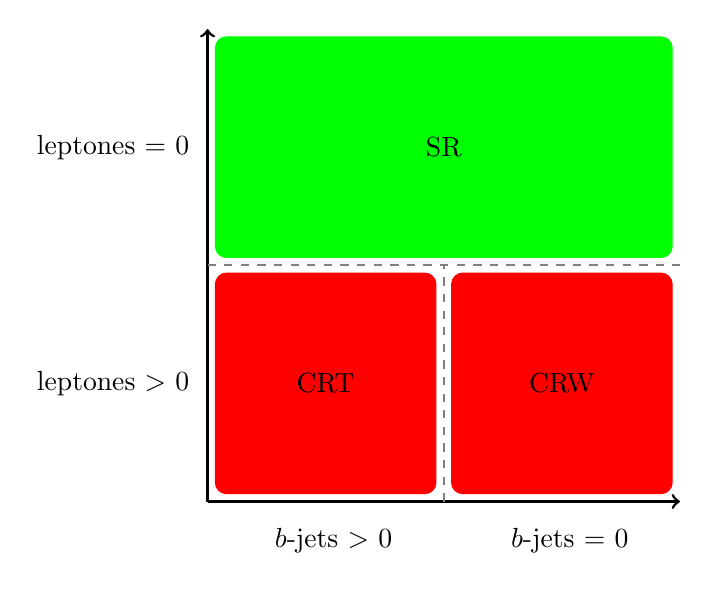
\begin{tikzpicture}[domain=0:4]

  \tikzstyle{region} = [rounded corners, fill]

  \draw[line width=1, ->] (0,0) -- (6,0);
  \draw[line width=1, ->] (0,0) -- (0,6);

  \draw[gray, dashed, line width=0.8] (0, 3.0) -- (6.0, 3.0);
  \draw[gray, dashed, line width=0.8] (3.0, 0) -- (3.0, 3.0);

  \draw node at (1.6,-0.5) {$b$-jets $>$ 0};
  \draw node at (4.6,-0.5) {$b$-jets = 0};
  \draw node at (-1.2, 1.5) {leptones $>$ 0};
  \draw node at (-1.2, 4.5) {leptones = 0};

  \draw[green, region] (0.1,3.1) rectangle (5.9,5.9);
  \draw node at (3.0,4.5) {SR};

  \draw[red, region] (0.1,0.1) rectangle (2.9,2.9) ;
  \draw node at (1.5,1.5) {CRT};

  \draw[red, region] (3.1,0.1) rectangle (5.9,2.9) ;
  \draw node at (4.5,1.5) {CRW};

\end{tikzpicture}
}

  \caption{Regiones de control definidas para normalizar el fondo de {\wgam} (CRW) y {\ttgam} (CRT). En este contexto <<leptón>> se refiere solo a electrones o muones.}
  \label{fig:bkg_crt_crw}
\end{figure}



\begin{table}[!htbp]
  \centering

  \caption{Selección para las regiones de control utilizadas para normalizar los
    fondos de {\wgam}, {\ttgam} y {\gjet}, asociadas a las regiones de señal
    {\SRL} y {\SRH}}
  \label{tab:bkg_crs}

  \begin{tabularx}{\textwidth}{r|CCC|CCC}

    \hline
                                     & \multicolumn{3}{c|}{\SRL} & \multicolumn{3}{c}{\SRH} \\
    \cline{2-7}
                                     &      \CRWL &      \CRTL &  \CRQL &     \CRWH &    \CRTH  &   \CRQH \\
  \hline
  $\pt^\gamma$ [\gev] $>$            &        125 &        125 &    125 &       150 &      150  &     300 \\
  $N_\mathrm{leptones}$              &          1 &    $\ge 1$ &      0 &         1 &  $\ge 1$  &       0 \\
  {\met} [\gev]                      &  [100-200] &   [80-200] &  $<50$ &  [100-200] & [80-200] &   $<50$ \\
  $N_\mathrm{jets} \ge$              &          4 &          4 &      4 &         2 &        2  &       2 \\
  $N_{b\text{-jets}}$                &          0 &    $\ge 1$ &      - &         0 &  $\ge 1$  &       - \\
  $\pt^{j_1},\pt^{j_2}$ [\gev] $>$   &        100 &        100 &    100 &        40 &       40  &      40 \\
  $\dphijm >$                        &        0.4 &        0.4 &    0.4 &       0.4 &      0.4  &     0.4 \\
  $\rt <$                            &          - &          - &   0.85 &         - &        -  &       - \\
  {\HT} [\gev] $>$                   &          - &          - &      - &         - &        -  &   $800$ \\
  $\dphijg <$                        &          - &          - &      - &       2.0 &      2.0  &     2.0 \\
  \hline
  \end{tabularx}

\end{table}


%% As seen in \Fig \ref{fig:sig_CR}, the signal contamination in the CRs is
%% expected to be small. For CRM, the low \MET cut kills most of the signal events,
%% keeping its fraction below 0.5\% across the whole grid and decreasing with the
%% gluon mass.

%% ## CRLW_2
%% Percentage of wgamma:  63.26 % 3.81429171562 / 6.02966526151
%% Largest contamination:  41.84 %
%% ## CRLW_3
%% Percentage of wgamma:  69.18 % 15.5461444855 / 22.4714100622
%% Largest contamination:  11.3 %
%% ## CRLT_2
%% Percentage of ttbarg:  55.83 % 8.56628704071 / 15.3442126885
%% Largest contamination:  74.96 %
%% ## CRLT_3
%% Percentage of ttbarg:  60.23 % 14.3853740692 / 23.8827633113
%% Largest contamination:  40.28 %

Es importante que las CR no tengan una contaminación de señal y para tal fin se
aplica, además, un corte superior en {\met}. En {\CRW} y {\CRT} la contaminación
de señal en las CR es $<3\%$ para la mayor parte de la grid, aunque es mayor
(hasta 70\%) para algunos puntos de baja masa de gluino en {\CRTL} (ver
\cref{fig:bkg_cr_contamination}).

\begin{figure}[!htbp]
  \centering

  \includegraphics[width=0.46\textwidth]{signal_contamination_crwl}\hspace{1cm}
  \includegraphics[width=0.46\textwidth]{signal_contamination_crwh}

  \includegraphics[width=0.46\textwidth]{signal_contamination_crtl}\hspace{1cm}
  \includegraphics[width=0.46\textwidth]{signal_contamination_crth}

  \includegraphics[width=0.46\textwidth]{signal_contamination_crql}\hspace{1cm}
  \includegraphics[width=0.46\textwidth]{signal_contamination_crqh}


  \caption{Contaminación de señal esperada en las regiones de control {\CRW} (arriba),
    {\CRT} (medio) {\CRQ} (abajo) asociadas a {\SRL} (izquierda) y {\SRH} (derecha).}
  \label{fig:bkg_cr_contamination}
\end{figure}



\subsection{Regiones de validación}

Como se mencionó anteriormente, en la definición de las regiones de control,
algunos cortes fueron relajados, o directamente removidos respecto a las SR,
para incrementar el número de eventos en las mismas. Para validar la
extrapolación entre las CR y la SR, se definen ciertas regiones de validación,
imponiendo nuevamente los cortes de la SR, de a uno a la vez.

De esta forma se definen las siguientes regiones de validación para {\CRW} y
{\CRT}, donde la X se refiere a la correspondiente CR (W o T). La selección
detallada puede verse en \cref{tab:bkg_vrs1}.

\begin{description}
\item[\textbf{VRXM}]  igual que CRX pero con el corte en {\met} como en la SR.
\item[\textbf{VRXR}]  igual que CRX pero con el corte en {\rt} como en la {\SRL} (solo para {\SRL}).
\item[\textbf{VRXH}]  igual que CRX pero con el corte en {\HT} como en la {\SRH} (solo para {\SRH}).
\end{description}

\begin{table}[!htbp]
  \centering

  \caption{Selección para las regiones de validación utilizadas para validar la extrapolación
    de los fondos de {\wgam}, {\ttgam}, entre las CR a las regiones de señal
    {\SRL} y {\SRH}}
  \label{tab:bkg_vrs1}

  \resizebox{\textwidth}{!}{
  \begin{tabular}{r|cccc|cccc}
    \hline
                                       & \multicolumn{4}{c|}{\SRL} & \multicolumn{4}{c}{\SRH} \\
    \cline{2-9}
                             &       VRWM &       VRWR &     VRTM &      VRTR &     VRWM &       VRWH &     VRTM &      VRTH \\
  \hline
  $\pt^\gamma$ [\gev] $>$    &        125 &        125 &      125 &      125  &      150 &        150 &      150 &      150  \\
  $N_\mathrm{leptones}$      &          1 &          1 &  $\ge 1$ &  $\ge 1$  &        1 &          1 &  $\ge 1$ &  $\ge 1$  \\
  {\met} [\gev]              &     $>200$ &  [100-200] &   $>200$ &  [80-200] &   $>300$ &  [100-200] &   $>300$ &  [80-200] \\
  $N_\mathrm{jets} \ge$      &          4 &          4 &        4 &         4 &        2 &          2 &        2 &         2 \\
  $N_{b\text{-jets}}$        &          0 &          0 &  $\ge 1$ &   $\ge 1$ &        0 &          0 &  $\ge 1$ &   $\ge 1$ \\
  $\pt^{j_1},\pt^{j_2}$ [\gev] $>$     &        100 &        100 &      100 &       100 &       40 &         40 &       40 &        40 \\
  $\dphijm >$                &        0.4 &        0.4 &      0.4 &       0.4 &      0.4 &        0.4 &      0.4 &       0.4 \\
  $\rt <$                    &          - &       0.85 &        - &      0.85 &        - &          - &        - &         - \\
  {\HT} [\gev] $>$           &          - &          - &        - &         - &        - &        800 &        - &       800 \\
  \hline
  \end{tabular}
  }

\end{table}



\section{Producción de fotones directos (\gjet)}
\label{sec:bkg_gjet}

Por diseño, la probabilidad de que eventos de procesos de producción de fotones
directos ({\gjet}) pasen a la región de señal es
baja, ya que resulta raro que estos eventos tengan una gran cantidad de {\met}.
Sin embargo, esta energía faltante puede ser producida por la mala
reconstrucción de la energía de los jets, y debido a que la sección eficaz de
estos procesos es muy alta, puede resulta en una contaminación significativa.

Para determinar este fondo no es posible confiar plenamente en las simulaciones
MC, debido a que la baja cantidad de eventos similares a la señal implicaría
usar una muestra con una muy alto número de eventos que resulta dificultoso desde un
punto de vista computacional. Por este motivo se diseñó
una región de control dominada por eventos de {\gjet} a la que se llamó {\CRQ}.
Los detalles de la selección se pueden ver en la \cref{tab:bkg_crs}. Básicamente
es la misma selección que la SR pero requiriendo baja energía faltante ($\met <
50 \gev$).

%% La estimación final del fondo de fotones directos es obtenida entonces normalizando los
%% eventos de la muestra MC en esta region de control.
%% The final estimate for the prompt photon background is obtained by normalizing the Sherpa MC events passing a dedicated selection (CRM) defined
%% from the corresponding SR but at low {\met} ($< 50 \gev$). As expected,  CRM selects an enriched sample %of events with similar kinematics to the SR but enriched in
%% of QCD background events. The multijet contamination is independently estimated with the ratio method explained in sec \ref{sec:jetfakes}. %, is explicitly removed from the selected sample to avoid double counting in the global fit described in sec \ref{sec:fitconfig}
%% Some intermediate {\met} regions between 50 {\gev} and the SR cut are kept for validation purposes. Given the large jet multiplicty and \MET requirements in SR2 and SR3, respectively, the prompt photon background is
%% expected to be very small in both signal regions. However, its contribution is not negligible in the control and validation regions so it is important to get a good normalization estimate.

%% ## CRM_2
%% Percentage of photonjet_sherpa:  87.65 % 1224.78869629 / 1397.31749731
%% Largest contamination:  0.67 %

%% ## CRM_3
%% Percentage of photonjet_sherpa:  87.54 % 156.909103394 / 179.23669574
%% Largest contamination:  0.35 %

La contaminación de señal en esta región de control es despreciable, debido a
que la señal posee gran cantidad de energía faltante, como puede verse en la
\cref{fig:bkg_cr_contamination}.

%% \begin{figure}[!htbp]
%%   \centering
%%   \includegraphics[width=0.49\textwidth]{signal_contamination_crql}
%%   \includegraphics[width=0.49\textwidth]{signal_contamination_crqh}

%%   \caption{Contaminación de señal esperada en la región de control {\CRQ} asociada a {\SRL} (izquierda) y {\SRH} (derecha).}
%%   \label{fig:bkg_cr_contamination}
%% \end{figure}


%% \subsection{Comparación de generadores}

%% Acá comparación entre Pythia y Sherpa


\subsection{Regiones de validación}\label{sec:bkg_vrs2}

Con un conjunto de cortes de selección se definen regiones para validar los resultados de la
extrapolación de {\gjet} de la región de control a bajo {\met} hasta
las SR a alto {\met}. Las regiones de validación deben estar lo más cerca posible
de las SR en el espacio de observables, pero deben ser ortogonales a las mismas.
Esto se logra invirtiendo algunos cortes, como se describe a continuación.

\begin{description}\itemsep0.1cm
\item[{\bf VRMX}] igual a la SR pero con un requerimiento intermedio en {\met}
  ($X\gev < \met < 150\gev$) con $X = 75,100$. El corte superior asegura la
  ortogonalidad con la SR.
\item[{\bf VRH}] igual a la SR pero invirtiendo el corte en {\HT} ($\HT<
  800\gev$). Solo definida para {\SRH}, ya que no hay un corte en {\HT} en
  {\SRL}.
\item[{\bf VRQ}] igual a la SR pero invirtiendo el corte en {\dphijm} ($\dphijm < 0.4$)
  para aumentar la contribución de fondos con {\met}
  instrumental.
\end{description}

En la \cref{fig:bkg_crq} pueden verse los esquemas de la definición de las CR y VR.

\begin{figure}[!htbp]
  \centering

  \resizebox{0.49\textwidth}{!}{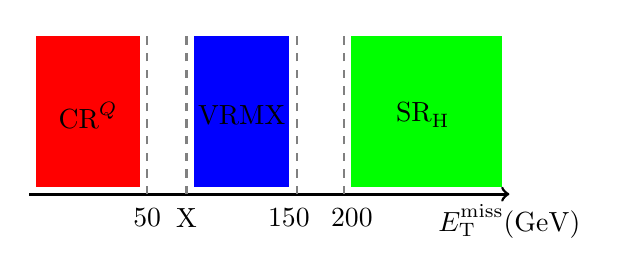
\begin{tikzpicture}[domain=0:4]

  \tikzstyle{region} = [fill]

  \draw[line width=1, ->] (0,0) -- (6.1,0) node[below] {$E_\mathrm{T}^\mathrm{miss} (\mathrm{GeV})$};
  %% \draw[line width=1, ->] (0,0) -- (0,3.1);

  \draw[gray, dashed, line width=0.8] (1.5, 0) -- (1.5, 2.1);
  \draw[gray, dashed, line width=0.8] (4.0, 0) -- (4.0, 2.1);
  \draw[gray, dashed, line width=0.8] (2.0, 0) -- (2.0, 2.1);
  \draw[gray, dashed, line width=0.8] (3.4, 0) -- (3.4, 2.1);

  \draw node at (1.5,-0.3) {50};
  \draw node at (2.0,-0.3) {X};
  \draw node at (3.3,-0.3) {150};
  \draw node at (4.1,-0.3) {200};

  \draw[green, region] (4.1,0.1) rectangle (6,2);
  \draw node at (5.0,1) {\SRL};

  \draw[red, region] (0.1,0.1) rectangle (1.4,2) ;
  \draw node at (0.75, 1) {\CRQ};

  \draw[blue, region] (2.1,0.1) rectangle (3.3,2) ;
  \draw node at (2.7,1) {VRMX};


\end{tikzpicture}
}
  \resizebox{0.49\textwidth}{!}{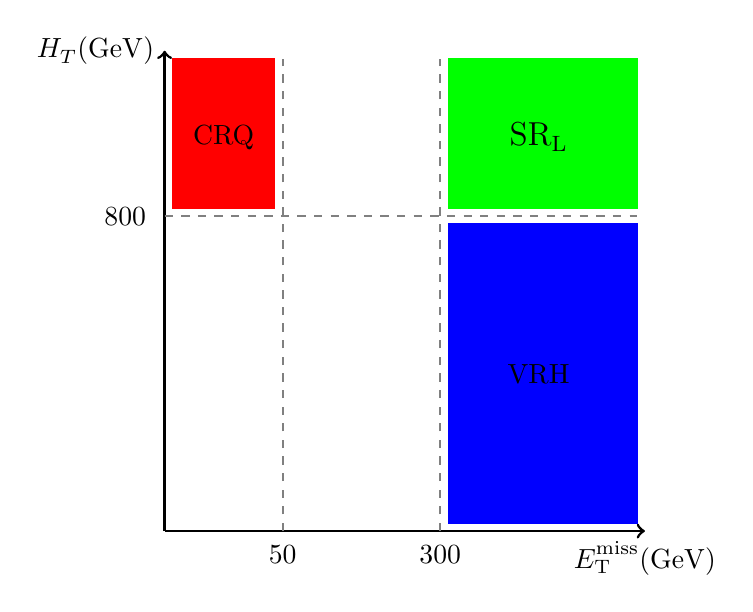
\begin{tikzpicture}[domain=0:4]

  \tikzstyle{region} = [fill]


  \draw[line width=1, ->] (0,0) -- (0,6.1) node[left] {$H_T (\mathrm{GeV})$};
  \draw[line width=1, ->] (0,0) -- (6.1,0) node[below] {$E_\mathrm{T}^\mathrm{miss} (\mathrm{GeV})$};

  %% \draw[gray, dashed, line width=0.8] (0, 2.5) -- (6, 2.5);
  \draw[gray, dashed, line width=0.8] (0, 4.0) -- (6, 4.0) node[black] at (-0.5,4.0) {800};
  \draw[gray, dashed, line width=0.8] (1.5, 0) -- (1.5, 6) node[black] at (1.5,-0.3) {50};
  \draw[gray, dashed, line width=0.8] (3.5, 0) -- (3.5, 6) node[black] at (3.5,-0.3) {300};

  \draw[green, region] (3.6,4.1) rectangle (6,6);
  \draw node at (4.75,5.0) {\large \SRH};

  \draw[red, region] (0.1,4.1) rectangle (1.4,6) ;
  \draw node at (0.75, 5) {CRQ};

  \draw[blue, region] (3.6,0.1) rectangle (6,3.9) ;
  \draw node at (4.75,2.) {VRH};

\end{tikzpicture}
}

  \caption{Esquema de las regiones de control diseñadas para normalizar el fondo
    de {\gjet} para {\SRL} (izquierda) y {\SRH} (derecha). También se muestran
    las regiones de validación utilizadas para validar la extrapolación
    $\mathrm{CR}\to\mathrm{SR}$.}
  \label{fig:bkg_crq}
\end{figure}



%----------------
% Electron fakes
%----------------
\section{Electrones identificados como fotones} \label{sec:efakes}

Los eventos en los que un electrón de alto {\pt} es identificado como un
fotón \cite{Bocci:1643300} pueden contaminar alguna de las SR. Esta contaminación
proviene generalmente de procesos del SM como $W(\to e\nu)$+ jets, $Z(\to ee)$ +
jets y {\ttbar}.

Como se mencionó en la \cref{sec:obj_photons}, los electrones y fotones dejan
lluvias electromagnéticas muy similares en el detector. Los algoritmos de
reconstrucción de fotones están diseñados para reducir la identificación errónea
de electrones como fotones aunque, para poder mantener una alta eficiencia de
reconstrucción, no se realiza una distinción demasiado estricta. En caso de
duda, los clusters electromagnéticos son reconstruidos bajo ambas hipótesis
(electrón o fotón) y guardados (duplicados) en ambas categorías. Esto implica
que algunos electrones pueden terminar siendo reconstruidos como fotones, y si
estos pasan la selección de fotones utilizada en el análisis, contribuirán al
fondo por mala identificación $e\to\gamma$.

Los electrones son reconstruidos a partir de los clusters asociados a una traza,
mientras que los fotones son reconstruidos de los clusters que no tienen ninguna
traza asociada (candidatos a fotones no-convertidos) o están asociados a un
vértice de conversión (candidatos a fotones convertidos). Se consideran los
vértices con una o dos trazas en la reconstrucción de fotones convertidos, y por
lo tanto los fotones convertidos pueden ser categorizados como fotones
convertidos con una traza o dos trazas. La traza de los candidatos a fotón
convertidos con una sola traza debe poseer un impacto en la \emph{B-layer}. Se
espera que una fracción de electrones pueda ser reconstruida como fotones
convertidos, por ejemplo, si falla la asociación de la traza a un impacto en la
B-layer, o si se asocia un vértice de conversión espurio a ella. Asimismo, el
electrón puede ser reconstruido como un fotón no-convertido si falla el
algoritmo que asocia la traza al cluster .

La fracción de electrones reconstruidos como fotones, depende claramente del
material en el detector, es por eso que pueden existir diferencias si se calcula
a partir de simulaciones Monte Carlo, ya que el material en las simulaciones no
es perfecto. Por tal motivo se calcula a partir de los datos, aunque también se
realiza una comparación con las muestras MC.
El número de eventos de electrones reconstruidos como fotones en la región de
señal ($N_{e\to\gam}^{\mathrm{SR}}$) se obtiene multiplicando esta fracción (\feg)
por el número de eventos en la muestra de electrones
obtenida invirtiendo el rol de fotones y electrones en la selección de la región
de señal ($N_e^{\mathrm{SR}}$). Para calcular este número de eventos se requiere
un electrón aislado de alto {\pt}, y los fotones de señal son
vetados.

\begin{equation}
  N_{e\to\gam}^{\mathrm{SR}} = \feg \cdot N_e^{\mathrm{SR}}
\end{equation}

Para estimar {\feg} se utiliza un método llamado \emph{tag and probe}, en una muestra
de eventos de datos {\Zee} que pasan el mismo trigger de fotones que utiliza el
análisis y la misma preselección. Adicionalmente, se
aplica un corte de $\met < 40 \gev$ para reducir la posible contaminación de
fotones reales de eventos de {\wgam}.

El método consiste en seleccionar un electrón (el electrón \emph{tag}) que
pasa un criterio de identificación \emph{tight} y que tiene $20 \gev < \pt < 125 \gev$.
Luego se busca un segundo candidato a electrón o fotón
(el objeto \emph{probe}). Este puede ser un electrón \emph{tight} o un fotón
\emph{tight}, ambos con $\pt > 125\gev$ y satisfaciendo los requerimientos de
aislamiento correspondientes.

Los valores de la masa de los pares de objetos seleccionados son guardados
separadamente para los tres casos posibles: dos electrones, un electrón y un
fotón convertido, o un electrón y fotón no-convertido. En los tres casos se
puede ver un pico alrededor del valor de la masa del bosón $Z$ ($\sim 91
\gev$).
Como el bosón $Z$ no puede decaer directamente en un electrón y un fotón, los
pares electrón-fotón que aparecen bajo el pico del $Z$ corresponden a electrones
mal identificados. Sin embargo, lo mismo aplica a otros procesos que contienen
dos electrones en estado final.
Por lo tanto es necesario utilizar algún método de
sustracción del fondo. Este deberá también tener en cuenta la contaminación por
las combinaciones aleatorias.

La probabilidad de identificación errónea {\feg} puede estimarse entonces como:

\begin{equation}\label{eq:efakerate}
  \feg = \frac{N_{e\gam}}{N_{ee}}
\end{equation}
%
donde $N_{e\gam}$ ($N_{ee}$) es el número de pares electrón-fotón
(electrón-electrón) encontrados en una ventana alrededor del pico del bosón $Z$ en la distribución de
la masa invariante, definida en el rango $81 < m_{ex} < 101 \gev$. Para obtener
el número de eventos $N_{ex}$, se realiza un ajuste de la distribución de la
masa invariante para los dos tipos de eventos utilizando un modelo de
señal+fondo. Este procedimiento se lleva a cabo de forma separada para fotones
convertidos y no-convertidos, y en clases del {\abseta} de los objetos
\emph{probe}. El bajo número de eventos disponibles hace imposible utilizar
clases de {\pt}, aunque de esta forma la estimación es conservativa ya que la
probabilidad de identificación errónea decrece con el {\pt} del electrón
\cite{Kuhl:1604846}.

Como modelo de señal se utiliza la suma de función \emph{Crystall-Ball} y una
Gausiana, mientras que para el modelo de fondo se utiliza un polinomio de grado
dos. En la \cref{fig:invmass_pairs} se pueden ver las distribuciones de la masa
invariante para pares de $ee$ y $e\gam$, para la selección inclusiva, y los
correspondientes ajustes del modelo.

\begin{figure}[!htb]
  \centering

  \includegraphics[width=0.49\textwidth]{figures/Fit_mee_efakes_Data_all}
  \includegraphics[width=0.49\textwidth]{figures/Fit_meg_efakes_Data_all}
  \caption{Distribuciones de la masa invariante de los pares de
    electrón-electrón (izquierda) y electrón-fotón (derecha). Se puede ver también el ajuste
    con el modelo de señal + fondo.}
  \label{fig:invmass_pairs}

\end{figure}

La probabilidad de identificación errónea se muestra en la \cref{fig:efake_eta},
como función del {\abseta} del objeto \emph{probe} para ``fotones'' convertidos
y no-convertidos. Este factor crece con {\abseta}, dado que está relacionado
con el incremento en el material del detector atravesado por los electrones y el
incremento en la tasa de reconstrucción de fotones convertidos con una sola
traza.

El {\feg} calculado a partir de los datos es comparado con el calculado a partir
de muestras MC de eventos de {\Zee} producidas con los generadores {\sherpa} y
{\powheg}. Se encuentra un buen acuerdo para todos los casos dentro de sus incertezas.
Los valores calculados de {\feg} pueden verse en la \cref{tab:efake_eta}, y \cref{tab:efake_uc} para fotones
convertidos y no-convertidos de forma separada.

\begin{figure}[!htb]
  \centering

  \includegraphics[width=0.45\textwidth]{figures/fegc_feta}
  \includegraphics[width=0.45\textwidth]{figures/fegu_feta}

  \caption{Probabilidad de que un electrón real sea identificado como un fotón convertido (izquierda)
    y un fotón no-convertido (derecha), como función de la pseudo-rapidez del objeto \emph{probe}. El valor
    calculado a partir de los datos es comparado con el valor calculado con las muestras MC de eventos de {\Zee} utilizando
    dos generadores distintos.}
  \label{fig:efake_eta}
\end{figure}


\begin{table}[!htb]
  \centering
  \caption{Probabilidad de que un electrón real sea identificado como un fotón
    como función de la pseudo-rapidez del objeto \emph{probe}. El valor
    calculado a partir de los datos es comparado con el valor calculado con las
    muestras MC de eventos de {\Zee} utilizando dos generadores distintos.}
  \label{tab:efake_eta}

  \begin{tabularx}{0.9\textwidth}{CCCC}
    \hline
                          & Datos             &  MC {\Zee} (\sherpa) & MC {\Zee} (\powheg) \\
    \hline
    $0 < |\eta| < 0.8$    & $0.014 \pm 0.002$ & $0.012 \pm 0.001$ & $0.014 \pm 0.002$ \\
    $0.8 < |\eta| < 1.52$ & $0.018 \pm 0.003$ & $0.014 \pm 0.001$ & $0.011 \pm 0.003$ \\
    $1.52 < |\eta| < 2.5$ & $0.033 \pm 0.006$ & $0.027 \pm 0.002$ & $0.032 \pm 0.006$ \\
    Inclusivo             & $0.019 \pm 0.001$ & $0.016 \pm 0.001$ & $0.017 \pm 0.002$ \\
    \hline
  \end{tabularx}

\end{table}

\begin{table}[!htb]
  \centering
  \caption{Probabilidad de que un electrón real sea reconstruido como un fotón
    convertido ($f_{e\to \gamma_c}$) o no-convertido ($f_{e\to \gamma_u}$).
    El valor calculado a partir de los datos es comparado con el valor calculado
    con las muestras MC de eventos de {\Zee}, utilizando dos generadores distintos.}
  \label{tab:efake_uc}

  \begin{tabularx}{0.9\textwidth}{CCCC}

    \hline
                       & Datos              & MC {\Zee} (\sherpa)        & MC {\Zee} (\powheg)        \\
    \hline
    $f_{e\to \gamma_u}$ & $0.007 \pm 0.001$ & $0.005 \pm 0.001$ & $0.005 \pm 0.001$ \\
    $f_{e\to \gamma_c}$ & $0.013 \pm 0.001$ & $0.011 \pm 0.001$ & $0.011 \pm 0.002$ \\
    $f_{e\to \gamma}$   & $0.019 \pm 0.001$ & $0.016 \pm 0.001$ & $0.017 \pm 0.002$ \\
    \hline
  \end{tabularx}

\end{table}


Para estimar la incerteza sistemática del método utilizado, el factor {\feg} fue
calculado variando el tamaño de la ventana de masa del $Z$, y sin la sustracción
del fondo. Como se aprecia en la \cref{tab:efake_syst} la mayor variación se
obtine en el caso de no realizar la sustracción del fondo y por lo tanto se
utiliza este valor como la incerteza sistemática del método, a pesar de que
resulta el límite más desfavorable.

\begin{table}[!htb]
  \centering
  \caption{Probabilidad de que un electrón real sea reconstruido como un fotón
    convertido o no-convertido, para variaciones del método original.}
  \label{tab:efake_syst}

  \begin{tabularx}{0.9\textwidth}{CCCC}
    \hline
            &  $m_{ee} \in [71, 111] \GeV$ & $m_{ee} \in [86,96] \gev$ & Sin sustracción del fondo  \\
    \hline
    $f_{e\to \gamma_u}$ & $0.007 \pm 0.001$ & $0.007 \pm 0.001$ & $0.012 \pm 0.001$ \\
    $f_{e\to \gamma_c}$ & $0.013 \pm 0.001$ & $0.012 \pm 0.001$ & $0.012 \pm 0.001$ \\
    $f_{e\to \gamma}$   & $0.019 \pm 0.001$ & $0.019 \pm 0.001$ & $0.024 \pm 0.001$ \\
    \hline
  \end{tabularx}

\end{table}


El valor calculado del factor de identificación errónea de electrón en fotón
({\feg}) resulta entonces el que se muestra en la \cref{tab:efake_final}.

\begin{table}[!htb]
  \centering

  \caption{Probabilidad de que un electrón real sea reconstruido como un fotón {\feg}, como función de $\eta$, junto
    con su incerteza estadística y sistemática.}
  \label{tab:efake_final}

  \begin{tabularx}{0.75\textwidth}{CC}

    \hline
     Región                &  $f_{e\to \gamma}$  \\
    \hline
      $0 < |\eta| < 0.8$     & $  0.014 \pm 0.002 \stat\ \pm 0.005 \syst\ $ \\
      $0.8 < |\eta| < 1.52$  & $  0.018 \pm 0.003 \stat\ \pm 0.004 \syst\ $ \\
      $1.52 < |\eta| < 2.5$  & $  0.033 \pm 0.006 \stat\ \pm 0.008 \syst\ $ \\
    \hline
  \end{tabularx}

\end{table}


En la {\SRL} se observaron 28 eventos que pasaban la selección al invertir el
rol de fotón y electrón, lo que corresponde a una estimación del fondo de
$N^{\SRL}_{e\to\gamma} = 0.38\, \pm\, 0.10$. En {\SRH}, dado el alto corte en
{\met}, no se observó ningún evento en la muestra de electrones.



%-----------
% Jet fakes
%-----------
\section{Jets identificados como fotones}
\label{sec:jfakes}

Los jets pueden ser identificados como fotones si tienen uno o dos {\pizero} con
alto {\pt} como partícula \emph{leading}, resultando en un objeto
electromagnético indistinguible de un fotón muy energético. Este fondo
proviene mayoritariamente de multijets, {\wjets} y eventos {\ttbar} decayendo
semi-leptónicamente, y puede ser una fuente importante de contaminación debido a
la gran sección eficaz de producción de estos procesos. Como la proporción de
jets mal identificados como fotones no está bien descripta por el MC, se
utiliza un método especialmente desarrollado a partir de los datos para su estimación.
La idea consiste en utilizar las diferencias en la distribución de energía de aislamiento
esperada para fotones reales y falsos, como se describe a continuación.

\subsection{Descripción del método}

Para reducir significativamente el fondo proveniente de jets, en el análisis se
utilizan fotones que satisfacen un criterio de selección \emph{tight}, como se
describe en \cref{sec:obj_photons}. Esta selección es inclusiva respecto a los
fotones reales, tiene una moderada contaminación de jets y es, por definición,
un criterio más ajustado que el trigger de fotones utilizado para la toma de los
datos. Por esta razón, hay una suficiente cantidad de candidatos a fotones
provenientes de jets que fallan la selección \emph{tight} pero satisfacen una
selección intermedia. Estos jets más similares a un fotón real, denominados
\emph{pseudo-fotones}, son útiles para modelar los jets que pasan la selección
total y la fracción de esta contaminación.

%Pseudo-photons are here defined as those passing the loose identification
%but failing (at least) one of a set of tight identification cuts. %, also known as {\it loose'-non-tight}.

La muestra de fotones que pasan los criterios de selección \emph{tight}
($N_{tight}$) contiene, en general, fotones reales ($N_{\gamma}$) y falsos
($N_{j\to\gamma}$), es decir, $N_{tight} = N_{\gamma} + N_{j\to\gamma}$.
Las distribuciones de la energía de aislamiento para estas
dos contribuciones van a tener formas diferentes, lo que puede ser explotado
para estimar ambas contribuciones. Para tal fin, se ajusta la distribución
total de energía de aislamiento con un combinación de modelos de señal y fondo.

El número de eventos de fotones falsos que pasa la identificación de fotones y
el corte de aislamiento puede ser estimado entonces integrando la componente de
fondo del ajuste sobre el rango de la región de señal ($\etiso<5\GeV$). De esta
forma la proporción de jets mal identificados como fotones, \fjg, resulta:

\begin{equation}\label{eq:jfake_formula}
  f_{j\to \gamma} = \frac{\int_{-\infty}^{5\gev} B(x)\, dx}{\int_{-\infty}^{5\gev} \left[S(x)+B(x)\right]\, dx}
\end{equation}
%
donde $x$ es la variable de energía de aislamiento \etiso, y $S(x)$ y $B(x)$ son
las distribuciones de señal y fondo en el ajuste combinado, respectivamente.
Esta fracción de fotones falsos es estimada en una región lo más cercana posible
a las regiones de señal, y luego utilizada para estimar el número de eventos
provenientes de jets mal identificados, pesando la muestra de fotones en la SR.




\subsection{Modelo de Señal} \label{sec:jfake_sig_template}

El modelo de señal se extrajo a partir de electrones provenientes de eventos de datos {\Zee}
utilizando el hecho que los
electrones y fotones dejan una señal similar en el calorímetro
electromagnético. La muestra de electrones es obtenida de eventos que satisfacen
el siguiente conjunto de cortes, después de haber pasado la preselección
descripta en \cref{sec:preselection}:

\begin{itemize}\itemsep0.1cm
\item Trigger de electrones %% (\texttt{2e12Tvhi\_loose}, \texttt{e24vhi\_medium} o \texttt{e60\_medium}).
\item Dos electrones \emph{medium}, aislados, con carga opuesta, y con $\pt>50,25\gev$
\item \MET\ $<40\gev$
\item $81\gev<m_{ee}<101\gev$
\end{itemize}

Después de aplicar los cortes anteriores, la contaminación de fondos no
provenientes del decaimiento del $Z$ es despreciable y, en particular, para eventos
de {\ttbar} resulta menor al $1\%$.

\begin{figure}[!htb]
  \centering

  \includegraphics[width=0.49\textwidth]{electron_iso_vs_pt_Zee_raw}

  \caption{Distribución de la energía de aislamiento ({\etiso}) de electrones provenientes
    de eventos {\Zee} en datos y MC, en función de {\pt}.}
  \label{fig:isolation_vs_pt}
\end{figure}

La \cref{fig:isolation_vs_pt} muestra el valor medio de la distribución de la energía de
aislamiento para los electrones seleccionados como función del {\pt} del
electrón en eventos de datos y simulaciones MC. De la figura resulta evidente que
para los datos existe una clara dependencia de {\etiso} con {\pt}, que no es el caso
para las simulaciones MC.
Para corregir esta dependencia residual con {\pt} se realiza un ajuste lineal de los
datos del cual se obtiene un factor de corrección que luego es aplicado a {\etiso}.
El valor del factor de corrección
obtenido en el ajuste en el rango $50<\pt<500 \gev$ es $0.00262 \pm 0.00008$.

En la \cref{fig:isolation_wandwo_correction} se muestra una comparación entre
datos y simulaciones del perfil de {\etiso} antes y después de la corrección. Se
puede ver que el acuerdo entre datos y MC es mucho mejor después de aplicar la
corrección.


\begin{figure}[!htb]
  \centering

  \includegraphics[width=0.49\textwidth]{electron_iso_Zee_raw}
  \includegraphics[width=0.49\textwidth]{electron_iso_Zee_corr}

  \caption{Comparación datos/MC de la distribución de {\etiso} de electrones
    provenientes de eventos {\Zee} (izquierda) y la correspondiente distribución
    después de aplicar la corrección por el {\pt} (derecha).}
  \label{fig:isolation_wandwo_correction}
\end{figure}

Para respaldar la estrategia de derivar el modelo de aislamiento de los fotones
a partir de electrones se realizaron varios estudios. Una validación importante
del método consistió en comparar la distribución de {\etiso} de electrones
provenientes de {\Zee} con los fotones provenientes del decaimiento radiativo
del $Z$ (\Zee\gam) que provee un fuente de fotones puros. Los eventos se
seleccionaron requiriendo el siguiente conjunto de cortes, después de la
preselección:

\begin{itemize}\itemsep0.1cm
\item Triggers de electrones %%(\texttt{2e12Tvhi\_loose1} o \texttt{e24vhi\_medium1} o \texttt{e60\_medium1})
\item Un fotón \emph{tight} aislado con $\pt>25 \gev$.
\item Dos electrones \emph{medium}, aislados, con carga opuesta, y con $\pt>50 \gev$ y $\pt>25 \gev$
\item $\Delta R(\gamma,l)>0.7$
\item \MET\ $<40\gev$
\item $40\gev<m_{ee}<85\gev$
\item $70\gev<m_{ee\gamma}<100\gev$
\end{itemize}

En la \cref{fig:photon_electron_iso} se presenta una comparación entre el modelo
de fotones reales de decaimientos radiativos del $Z$ y electrones de {\Zee}. El
gráfico a la derecha es obtenido después de remover la dependencia con el {\pt}
con el factor de corrección como se describió anteriormente. Puede verse, a partir
del cociente en el panel inferior,
el buen acuerdo entre las distribuciones de {\etiso} de fotones y
electrones, en particular después de aplicar la corrección, dando confianza en la
hipótesis de usar electrones para modelar los fotones.

%% Vale la pena nota que el espectro de {\pt} de fotones tan bajo en estos
%% procesos (ver {\fig} \ref{fig:zllg_pt}) as compared to the generally broader electron \pt\ spectrum from Z decay. %of the electrons (see {\fig} \ref{fig:zeeg_pt}). \tosolve{add this last plot}

\begin{figure}[!htb]
  \centering

  \includegraphics[width=0.49\textwidth]{electronphoton_iso_Zee_before_correction}
  \includegraphics[width=0.49\textwidth]{electronphoton_iso_Zee_after_correction}

  \caption{Comparación de las distribuciones de la energía de aislamiento para fotones reales de
    decaimiento radiativo del $Z$ y electrones provenientes del decaimiento $\Zee$ antes (izquierda)
    y después (derecha) de la corrección por \pt.}
    \label{fig:photon_electron_iso}

\end{figure}

Para estudiar el efecto en las distribuciones obtenidas de {\Zee} en distintas
regiones cinemáticas, en la \cref{fig:electron_iso_HT}, se presentan las
distribuciones agregando un corte en {\HT} para eventos {\Zee} en muestras MC y
datos. Como es de esperar, la energía de aislamiento es más alta y la
distribución se hace más ancha con \HT. Desafortunadamente, la escasa
estadística impide el uso del corte en {\HT} de la SR. En cualquier caso, el
efecto se considera como una posible fuente de incerteza sistemática.

\begin{figure}[!htb]
  \centering

  \includegraphics[width=0.49\textwidth]{electron_iso_ZeeHMC_corr}
  \includegraphics[width=0.49\textwidth]{electron_iso_ZeeH_corr}

  \caption{Dependencia de la energía de aislamiento de electrones con {\HT}
    para MC (izquierda) y datos (derecha) \Zee}
    \label{fig:electron_iso_HT}

\end{figure}



\subsection{Modelo de fondo} \label{sec:jfake_bkg_template}

El modelo de fondo se obtuvo de los datos, en eventos que pasan todos los
criterios de identificación salvo los criterios de identificación \emph{tight}
de fotones. La muestra de pseudo-fotones seleccionada de esta forma debe
presentar un perfil de aislamiento similar a la de fotones reales, permitiendo
una pequeña contaminación de señal y alta estadística.

Se realizó un estudio detallado en muestras MC para encontrar el mejor conjunto
de los cortes utilizados por el criterio de identificación \emph{tight} que debía ser
revertido para modelar de la mejor manera la distribución de aislamiento para
los fotones falsos provenientes de decaimientos de hadrones en la SR. En la
\cref{fig:jetfake_mc_data} se puede ver la comparación de dos definiciones
distintas de pseudo-fotones para MC y datos.
Los pseudo-fotones \emph{loose-non-tight} pasan los cortes de
identificación \emph{loose}, pero fallan al menos uno de los cortes
\emph{tight}. A pesar de la escasa estadística, resulta claro que falla en su
objetivo de modelar el fondo tanto en datos como en MC. Se obtiene un mejor
acuerdo para la definición \emph{loose'-non-tight}, en la cual los
fotones pasan todos los cortes \emph{tight} salvo (al menos) uno de las
variables en la sección de bandas del calorimetro ($F_\text{side}$, $w_{s3}$, $E_\text{ratio}$,
$\Delta E$). Estas variables son construidas con solo algunas bandas centrales
alrededor de la dirección del fotón, y por lo tanto se espera que no tengan una
correlación con la energía de aislamiento del fotón, ya que para el cálculo de
esta se excluye la energía en las celdas centrales para tener en cuenta la
propia energía del fotón. Utilizando esta definición, los pseudo-fotones tienen
un perfil de aislamiento con una forma similar a la de fotones \emph{tight} y
por lo tanto es posible la extrapolación a la SR.

\begin{figure}[!htb]
  \centering

  \includegraphics[width=0.49\textwidth]{figures/bkg_mc_pseudo_data_SR_l_ptbin}
  \includegraphics[width=0.49\textwidth]{figures/bkg_mc_pseudo_data_SR_lp_ptbin}

  \caption{Distribución de la energía de aislamiento para fotones falsos
    provenientes de decaimientos hadronicos (a nivel generador), comparada con
    la de pseudo-fotones obtenidos con dos definiciones diferentes: \emph{loose-non-tight} (izquierda)
    y \emph{loose'-non-tight} (derecha). Ver detalles en el texto.}
  \label{fig:jetfake_mc_data}

\end{figure}

Más aún, como se ve en la \cref{fig:jetfake_pseudo_data_pt}, los fotones \emph{loose'-non-tight}
reproducen mejor el espectro de {\pt} de los fotones \emph{tight}, y no es necesario
aplicar una correción por este motivo.

\begin{figure}[!htb]
  \centering

  \includegraphics[width=0.5\textwidth]{bkg_data_pseudo_tight_data_VR}

  \caption{Distribución del {\pt} del fotón para candidatos
    \emph{tight} y las dos definiciones diferentes de pseudo-fotones.}
  \label{fig:jetfake_pseudo_data_pt}

\end{figure}


La distribución de la energía de aislamiento de los pseudo-fotones puede variar
en distintas regiones cinemáticas. Es por esta razón que para derivar el modelo
de fondo se utiliza una región relajada (CRJ), cercana a las regiones de señal, definida en
la \cref{tab:cr_jetfake}. Para mantener esta región ortogonal a las SR, se
requiere un corte intermedio en {\met}, y algunos otros cortes son relajados
para ganar estadística. Como se espera, a mayor actividad hadrónica en el
evento, mayor es la energía de aislamiento del fotón. En la
\cref{fig:jetfake_pseudo_data_LR_VR} se puede ver las diferencias para distintos
requerimientos en {\HT}. En la región CRJ se utiliza un corte intermedio entre
ambas SR, y las posibles diferencias son tenidas en cuenta como incerteza
sistemática.


%% For this reason, the control region selection to derive the templates is kept close to the SR, as listed in {\tab} \ref{tab:cr_jetfake}.
%% An orthogonality requirement is placed on \MET ($50-150\gev$) and some SR cuts are loosened to retain statistics.
%% As expected, however, the larger the jet activity around the harder the photon isolation in the event. So the
%% \HT\ requirements can not be loosened much. This can be clearly observed in {\fig} \ref{fig:jetfake_pseudo_data_LR_VR},
%% for a loose (CRFJL: $>200 \gev$) and tight (CRFJ: $>600 \gev$) \HT\ selection. The latter is therefore used to
%% perform the combined fit and to compute the jet fake factor, as discussed in the next section.

\begin{table}[!htb]
  \centering

  \caption{Definición de la region utilizada para la estimación de los jets mal identificados como fotones.}
  \label{tab:cr_jetfake}

%%   %%$f_{j\to\gamma}$ fake factor derived in the CRFJ region. The numeric suffix indicates (when present) the SR associated to each region (SR2 or SR3).}
  \begin{tabular}{rc}
    \hline
                                            &           CRJ  \\ %       CRFJL \\
    \hline
    $\pt(\text{pseudo}-\gamma)$ [\gev] $>$ &           125 \\ %         125 \\
    $\nleptons$                              &             0 \\ %           0 \\
    \met [\gev]                              &   $[50, 150]$ \\ % $[50, 150]$ \\
    $\njets \ge$                             &             2 \\ %           2 \\
    $\pt^{j_1,j_2}$  [\gev]  $>$             &           100 \\ %         100 \\
    $\dphijm >$                              &           0.4 \\ %         0.4 \\
    \HT [\gev] $>$                           &           600 \\ %         200 \\
    \hline
  \end{tabular}

\end{table}



%% \begin{figure}[!htbp]
%%   \centering

%%   \includegraphics[width=0.49\textwidth]{figures/bkg_pseudo_data_SREB_l}
%%   \includegraphics[width=0.49\textwidth]{figures/bkg_pseudo_data_SREB_lp}

%%   \caption{Distribución de la energía de aislamiento para pseudo-fotones loose-non-tight (izquierda) y loose'-non-tight (derecha),
%%     luego de la selección CRFJ, en la regiones de \emph{barrel} y \emph{endcap}.}
%%   \label{fig:jetfake_pseudo_data_BE}

%% \end{figure}

\begin{figure}[!htbp]
  \centering

  \includegraphics[width=0.49\textwidth]{bkg_pseudo_data_SR_VR_l}
  \includegraphics[width=0.49\textwidth]{bkg_pseudo_data_SR_VR_lp}

  \caption{Distribución de la energía de aislamiento para pseudo-fotones \emph{loose-non-tight} (izquierda) y \emph{loose'-non-tight} (derecha),
    luego de la selección con un corte en $\HT>200 \gev$ y $\HT>600 \gev$.}
  \label{fig:jetfake_pseudo_data_LR_VR}

\end{figure}

Finalmente, se encuentra que la distribución de los pseudo-fotones está bien
descripta por una función \emph{Crystall-Ball}. La
distribución en datos y el ajuste puede verse en la \cref{fig:jetfake_sigbkg}.

%% The parametrized template is used in the combined
%% fit to tight photon data to derive the jet fake rate.

%% \begin{figure}[h]
%%   \begin{center}
%%   \includegraphics[width=0.49\textwidth]{iso_fit_bkg_wpars}
%%   \caption{Fit to the observed isolation template for  loose'-non-tight pseudo-photon data in the VR.}
%%   \end{center}
%%   \label{fig:jetfake_bkg_template_fit}
%% \end{figure}


\subsection{Ajuste combinado y estimación del fondo} \label{sec:jet_fake_results}

%% A template fit to both signal and background distributions is then used to model the shape of the photon isolation
%% for each contribution, as shown in \cref{fig:jetfake_sigbkg}, together with the fitted parameters.
%The corresponding $\chi^2$/dof are 2.4 and 8.8 for signal and background templates with 240 points.

A fin de modelar la forma de la energía de aislamiento de los fotones \emph{tight} en los datos,
se utiliza el modelo de señal y fondo descriptos en las secciones anteriores, como se puede
apreciar en la \cref{fig:jetfake_sigbkg}.
La distribución de {\etiso} para todos los eventos que pasan los criterios de
selección de la región relajada CRJ es ajustada a una combinación lineal de
los modelos de señal y fondo. El ajuste combinado y cada componente de la
distribución pueden verse en \cref{fig:jetfake_combfit}. Los parámetros son
inicializados con los valores extraídos de los ajustes individuales a la señal y
el fondo, y se los permite variar dentro de su incerteza

%As this fit is the source of the biggest systematic uncertainty the range of the parameters is then extend to two times the
%individual fit uncertainties to compute the systematic of the method.

Para estimar la incerteza sistemática, el ajuste combinado es realizado
sin ninguna limitación en los parámetros. La incerteza obtenida es del
50\% del valor de $f_{j\to\gamma}$, lo suficientemente grande para contener
cualquier potencial inexactitud en el modelado de la señal y el fondo.

%The fitted parameters for the signal, background and combined fits are tabulated in \Tab \ref{tab:jetfake_fit_pars}.
%% Los parametros estimados del ajuste combinado estan tabulados en la
%% \cref{tab:jetfake_fit_pars}.

El número de fotones total (N$_\text{total}$) y falsos
(N$_{j\to\gamma}$) esperados es obtenido
integrando las componentes de fondo y total del ajuste combinado sobre todo el
rango $\etiso<5\gev$, respectivamente:

\begin{itemize}
\item[] N$_{j\to\gamma}= 24143 \pm 56$

\item[] N$_\text{total} = 281813 \pm 586$
\end{itemize}

La fracción $f_{j\to \gamma}$ es obtenida simplemente como el cociente
en la \cref{eq:jfake_formula}:

\begin{itemize}
\item[] $f_{j\to\gamma} = 0.0857 \pm 0.0003 \stat \pm 0.04 \;\syst$
\end{itemize}

\begin{figure}[!htb]
  \centering

  \includegraphics[width=0.49\textwidth]{iso_fit_sig_wpars}  \hfill
  \includegraphics[width=0.49\textwidth]{iso_fit_bkg_wpars}

  \caption{Ajuste a las distribuciones de {\etiso} de señal
    (izquierda) y fondo (derecha) (derecha) en la región
    relajada CRJ.}
  \label{fig:jetfake_sigbkg}

\end{figure}

\begin{figure}[!htb]
  \centering

  \includegraphics[width=0.49\textwidth]{iso_fit_sarange}

  \caption{Ajuste combinado a la distribución de {\etiso}
    para los pseudo-fotones que pasan la selección de la región
    relajada CRJ (ver texto para detalles).}
  \label{fig:jetfake_combfit}

\end{figure}


El número de jets identificados erróneamente como fotones puede ser estimado
utilizando la fracción $f_{j\to\gam}$ como,

\begin{equation}\label{eq:njfakes}
  N_{j\to\gam} = f_{j\to\gam} \cdot N_\mathrm{tight}
\end{equation}

Para estimar la contribución en las SR, sin necesidad de utilizar el número de
eventos en las SR, lo que implicaría utilizar los datos en la region que se
utiliza para la búsqueda, se parametrizó este número como función de \met, como
se puede ver en \cref{fig:jetfake_nfakes_met}, utilizando una función
exponencial $N_{j\to\gam} = \exp(a+b \, \met)$ que luego se extrapola a la SR.
Los valores de $a$ y $b$ obtenidos del ajuste se muestran en la
\cref{tab:exppars}.

\begin{table}[!htbp]
  \centering
  \caption{Parámetros que resultan del ajuste a la distribución de $N_{j\to\gam}$ como función de {\met} con una función exponencial $\exp(a+b\, \met)$.}
  \begin{tabular}{crr}
    \hline
    Parámetro &  {\SRL} & {\SRH} \\
     \hline
     a & $3.87 \pm 1.25$  &  $1.80 \pm 0.98$ \\
     b &  $-0.054 \pm 0.018$  & $-0.047 \pm 0.014$ \\
     \hline
  \end{tabular}
  \label{tab:exppars}
\end{table}


La contaminación esperada de jets falsos en las SR se estima integrando la
parametrización de $N_{j\to\gam}$ sobre la región de {\met} de cada SR.

\begin{align}
  N_{j\to\gam}^\text{\SRL} &= \int_{200}^{\infty} N_\text{fakes}(\met) \, d\met = 0.01 \pm 0.02 \\
  N_{j\to\gam}^\text{\SRH} &= \int_{300}^{\infty} N_\text{fakes}(\met) \, d\met = 0.0001 \pm 0.0001
\end{align}

Debido a que las incertezas son de igual o mayor magnitud que los valores centrales,
se utilizaron los valores de estas como la estimación final en las SR.


\begin{figure}[!htbp]
  \centering
  \includegraphics[width=0.49\textwidth]{nfakes_srl}  \hfill
  \includegraphics[width=0.49\textwidth]{nfakes_srh}
  \caption{Parametrización del número de jets mal identificados como
    función de {\met} para {\SRL} (izquierda) y {\SRH} (derecha).}
  \label{fig:jetfake_nfakes_met}
\end{figure}

El fondo de jets identificados como fotones es estimado similarmente en las
regiones de control y validación,
multiplicando el número de eventos observado en cada caso por el factor
$f_{j\to\gamma}$.


%% The final background contamination expected from jets faking photons is obtained by weighting the number of events observed in data,
%% after the otherwise full tight SR selections detailed in sec \ref{sec:signal_regions} (i.e. only the photon identification requirement is reversed).


%% Indeed, no pseudo-photon event was ultimately observed after all CRJ selections. This leads to a
%% j$\to\gamma$ background estimate of $<0.07$ events. Consistently, MC studies have shown this
%% background to be small in the high \MET\ and \HT\ regimes on the final SRs. As seen in \Tab \ref{tab:mc_events_sr_phtype}, the
%% MC predicts a jet fake contamination of $0.10\pm 0.04$ and $0.02 \pm 0.02$ event for SR2 and SR3, respectively.
%% This supports the findings in the data, agreeing within the uncertainties. The final jet fake background yield is estimated as $N^\text{SR}_\text{jfakes} = 0.0^{+0.1}_{-0.0}$, which accommodates an extra $+0.03$ uncertainty from the comparison of the MC-data predictions.

%% \chapter{Determinación de las incertezas sistemáticas}

%% \chapter{Análisis Estadístico y Resultados}

En este Capítulo se presentan los resultados, y el analisis estadistico
de los datos. Como se explica en el \cref{cap:estadistica}, se utiliza
como estadistico de prueba el \emph{profile likelihood ratio}



Para el analisis estadistico se utiliza \texttt{HistFitter}[], una herrmienta
desarrollada dentro del grupo de SUSY en ATLAS, y es basicamente una interfaz
de \texttt{RooFit}, \texttt{RooStats}\cite{Moneta:2010pm} y
\texttt{HistFactory} \cite{Cranmer:1456844}, de forma de facilitar el analisis
estadistico. Ademas el hecho de utilizar una misma herramienta en distintos
analisis dentro de ATLAS, permite que su combinacion estadistica sea mas sencilla.


En este capítulo se presenta el análisis estadístico de los datos. La
compatibilidad con el Modelo Estándar, los limites en la sección eficaz y los
limites de exclusión son obtenidos utilizando el profile log likelihood ratio
LLR.


%% The profile LLR is obtained from a simultaneous fit to the contributions
%% from Standard Model background and supersymmetric signal
%% models in a given signal region and its associated background
%% control regions, which are all by design statistically independent.
%% Cross-contamination of backgrounds across control region
%% boundaries and the propagation of statistical and systematic uncertainties is cleanly taken into account.


% Cuando se realiza el ajuste simultaneo en las CR,
%% When fitting CRs simultaneously, common normalizations are allowed in order to correctly take into
%% account the other background contamination in a given CR. Experimental systematic uncertainties are
%% correlated across the CRs and a SR. Sample-dependent theory systematics are uncorrelated.


%% Cada función de Poisson $P_{i}$ refleja el numero de eventos medidos en la region $i$,
%% ${\mathbf n_{i}}$, y el n\'umero de eventos esperados para las componentes de se\~nal
%% ${\mathbf s}$ y fondo ${\mathbf b}$. El factor de normalización $\mu$ para los fondos
%% \wgamma, \ttbargam, y \gjet son parametros libres del fit.
%% Los otros fondos considerados en el ajuste son \vgamma\ (incluyendo \znunugam) y
%% \topgamma\ MC, y los estimados mediante data-driven para electrones y jet fakes
%% descriptos en el capitulo \ref{}.
%% Los parametros nuisance $\apha$ parametrizan las incertezas sistematicas en la se\~nal
%% y el fondo por medio de una funcion gausiana. El tratamiento de las incertezas
%% sistematicas se describe en la seccion \ref{}.


%% By the simultaneous fit to the data in CRs or to the data in CRs and in a SR, these free and nuisance
%% parameters above can  be optimized with proper correlations and errors. In addition, by constraining the
%% parameters on background components mainly by the control regions with large statistics, the impacts of
%% these uncertainties in the SRs are reduced.


%% \begin{itemize}
%% \item {\bf Discovery fit:} the SR is added to the fit together with a generic non-SM signal component, which is neglected in the CRs. The background prediction achieved is this
%% way conservative since any signal contribution in the CRs is attributed to background and thus results in a possible overestimation of the background in the SRs. As shown above, however, this contribution is expected to be negligible.
%% \item {\bf Exclusion fit} both CRs and SRs are used in the fit. The signal contribution is taken into account as predicted by the tested SUSY model in all the regions.
%% \end{itemize}



\section{Validación del Modelo o Ajuste de solo-fondo} \label{sec:bkgonlyfit}


%--------------
% Bkg-only fit
%--------------


% Control Regions
\subsection{Resultados en las regiones de control}

Para validar el modelo propuesto y la metods utilizados para estimar los fondos,
se realiza un ajute simultaneo utilizando unicamente las CR. De este ajuste se
obtienen los factores de normalizacion de los fondos {\wgam} ($\mu_Q$), {\ttgam}
($\mu_T$) y {\gjet} ($\mu_Q$).


Los resultados del ajuste y el numero de eventos en los datos observados se
presnetan en la \cref{tab:fit_result_vrl,tab:fit_result_vrh} para las distintas
regiones de validacion.

% The distributions of several selection variables in these regions are shown in \App \ref{sec:ap_before_after}, before and after the fit. The fitted background predictions agree well with the data event counts within the uncertainties. The normalization factors determined for \wgamma\ ($\mu_{W}$), \ttbargam\ ($\mu_{T}$) and QCD prompt photon production ($\mu_{Q}$) are shown in \Tab \ref{tab:fit_bkgonly_mus}. %The $\mu_{W}$ value is consistent
%% %% %with unity within uncertinties. %As expected, $\mu_{Q}$ is way smaller, since the statistics for the smeared pseudo-data is artificially enhanced.
%% The systematic uncertainties in the two signal regions  after the background fit are summarized in \Fig \ref{fig:fit_unc_nuisance_SR}. No profiling of the systematics uncertainties is observed. %hopefully
%% The correlations of these systematics uncertainties and the normalizations are shown in \Fig \ref{fig:fit_corr_SR}. % What do we observe here?

\begin{table}[!htbp]
  \centering

  \caption{Factores de normalización utilizados para normalizar los fondos
    {\wgam} ($\mu_{W}$), {\ttgam} ($\mu_{T}$) y {\gjet} ($\mu_{Q}$), obtenidos
    del ajuste combinado de las CR. Las incertezas mostradas son las
    del ajuste.}
  \label{tab:fit_bkgonly_mus}

  \begin{tabularx}{0.8\textwidth}{CCCC} %cccc}
    \hline
    &       $\mu_{Q}$ &       $\mu_{W}$ &       $\mu_{T}$ \\
    \hline
    {\bf \SRL} & $0.94 \pm 0.44$ & $1.34 \pm 0.89$ & $1.40 \pm 0.77$ \\
    {\bf \SRH} & $1.22 \pm 0.58$ & $1.24 \pm 0.39$ & $0.54 \pm 0.37$ \\
    \hline
  \end{tabularx}

\end{table}


\begin{table}[!htbp]
  \centering

  \caption{Resultados del ajuste en las CR correspondientes a {\SRL}, con una luminosidad integrada total de 20.3 \ifb.
    El numero de eventos observado es comparado con el numero de eventos esperado de fondo, despues de la correspondiente
    normalizacion en las CR. En la parte inferior de la tabla se muestran tambien lo valores nominales del fondo antes de
    la correspondiente normalizacion. Las incertezas incluyen la incerteza estadistica y sistematica.}
  \label{tab:fit_result_cr2}

  %\resizebox{\textwidth}{!}
  {\small\input{tables/table_SR2_CR.tex}}

\end{table}


\begin{table}[!htbp]

  \caption{Resultados del ajuste en las CR correspondientes a {\SRH}, con una luminosidad integrada total de 20.3 \ifb.
    El numero de eventos observado es comparado con el numero de eventos esperado de fondo, despues de la correspondiente
    normalizacion en las CR. En la parte inferior de la tabla se muestran tambien lo valores nominales del fondo antes de
    la correspondiente normalizacion. Las incertezas incluyen la incerteza estadistica y sistematica.}
  \label{tab:fit_result_cr3}

  \input{tables/table_SR3_CR.tex}

\end{table}


\begin{figure}[!htbp]
  \centering

  \includegraphics[width=0.49\textwidth]{can_crql_met_et_afterFit}
  \includegraphics[width=0.49\textwidth]{can_crql_rt4_afterFit} \\

  \includegraphics[width=0.49\textwidth]{can_crwl_met_et_afterFit}
  \includegraphics[width=0.49\textwidth]{can_crwl_rt4_afterFit} \\

  \includegraphics[width=0.49\textwidth]{can_crtl_met_et_afterFit}
  \includegraphics[width=0.49\textwidth]{can_crtl_rt4_afterFit} \\

  \caption{Distribuciones observadas en las regiones de control {\CRQL}, {\CRWL}
    y {\CRTL}, después del ajuste combinado.}
  \label{fig:bkgfit_crl_after}

\end{figure}


\begin{figure}[!htbp]
  \centering

  \includegraphics[width=0.49\textwidth]{can_crqh_met_et_afterFit}
  \includegraphics[width=0.49\textwidth]{can_crqh_rt4_afterFit} \\

  \includegraphics[width=0.49\textwidth]{can_crwh_met_et_afterFit}
  \includegraphics[width=0.49\textwidth]{can_crwh_rt4_afterFit} \\

  \includegraphics[width=0.49\textwidth]{can_crth_met_et_afterFit}
  \includegraphics[width=0.49\textwidth]{can_crth_rt4_afterFit} \\

  \caption{Distribuciones observadas en las regiones de control {\CRQH}, {\CRWH}
    y {\CRTH},  después del ajuste combinado.}
  \label{fig:bkgfit_CRh_after}

\end{figure}





%% Validation Regions
\subsection{Resultados en las regiones de validación}

\begin{table}[!htbp]

  \caption{Resultados del ajuste en las VR correspondientes a {\SRL}, con una luminosidad integrada total de 20.3 \ifb.
    El numero de eventos observado es comparado con el numero de eventos esperado de fondo, despues de la correspondiente
    normalizacion en las CR. En la parte inferior de la tabla se muestran tambien lo valores nominales del fondo antes de
    la correspondiente normalizacion. Las incertezas incluyen la incerteza estadistica y sistematica.}
  \label{tab:fit_result_vr2}

  \input{tables/table_SR2_VR.tex}

\end{table}


\begin{table}[!htbp]

  \caption{Resultados del ajuste en las VR correspondientes a {\SRH}, con una luminosidad integrada total de 20.3 \ifb.
    El numero de eventos observado es comparado con el numero de eventos esperado de fondo, despues de la correspondiente
    normalizacion en las CR. En la parte inferior de la tabla se muestran tambien lo valores nominales del fondo antes de
    la correspondiente normalizacion. Las incertezas incluyen la incerteza estadistica y sistematica.}
  \label{tab:fit_result_vr3}

  \input{tables/table_SR3_VR.tex}

\end{table}


\begin{figure}[!htbp]
  \centering

  \includegraphics[width=0.49\textwidth]{figura}
  \includegraphics[width=0.49\textwidth]{figura} \\

  \includegraphics[width=0.49\textwidth]{figura}
  \includegraphics[width=0.49\textwidth]{figura} \\

  \includegraphics[width=0.49\textwidth]{figura}
  \includegraphics[width=0.49\textwidth]{figura} \\

  \caption{Distribuciones observadas en las regiones de validación, después del ajuste combinado.}
  \label{fig:bkgfit_crl_after}

\end{figure}


\begin{figure}[!htbp]
  \centering

  \includegraphics[width=0.49\textwidth]{figura}
  \includegraphics[width=0.49\textwidth]{figura} \\

  \includegraphics[width=0.49\textwidth]{figura}
  \includegraphics[width=0.49\textwidth]{figura} \\

  \includegraphics[width=0.49\textwidth]{figura}
  \includegraphics[width=0.49\textwidth]{figura} \\

  \caption{Distribuciones observadas en las regiones de validación,  después del ajuste combinado.}
  \label{fig:bkgfit_CRh_after}

\end{figure}

\clearpage


\subsection{Parámetros del ajuste}

\begin{figure}[!htbp]
  \centering

  \includegraphics[width=\textwidth]{syst_pull_afterFit_SR2} \\
  \includegraphics[width=\textwidth]{syst_pull_afterFit_SR3}

  \caption{Resumen de los parametros despues del ajuste para {\SRL} (arriba) y {\SRH} (abajo).}
  \label{fig:fit_unc_nuisance_SR}

\end{figure}

\begin{figure}[!htbp]
  \centering

  \includegraphics[width=\textwidth]{figures/corrMatrix_SR2} \\
  \includegraphics[width=\textwidth]{figures/corrMatrix_SR3} \\

  \caption{Matriz de correlacion de los parametros del ajuste, correspondientes a {\SRL} (arriba) y {\SRH} (abajo).}
  \label{fig:fit_corr_SR}

\end{figure}


%% The background predictions from the fit in SR2 and SR3 are presented in \Tab \ref{tab:fit_result_sr}. Both the nominal estimates
%% before the fit and the predicted yields from the background fits are shown.
%% No significant data deviation from the predicted background yields is observed in any of the SRs. The results after fit are
%% also shown for all regions in \Fig \ref{fig:fit_region_composition}.

%% The breakdown of systematic
%% uncertainties on the total background prediction are presented in \Tab \ref{tab:fit_result_sr2_syst} and \ref{tab:fit_result_sr3_syst}.
%% Since the individual uncertainties can be correlated and the negative correlations between normalizations (representing the
%% impact of the CR statistics on the total uncertainty) and systematic uncertainties are observed as expected, they
%% do not necessarily add up by quadrature to the total background uncertainty. The square
%% root of the number of the expected events are calculated in order to illustrate the relative impact of the
%% SR Poisson statistical uncertainties with respect to the total background uncertainties. The
%%  relative systematic uncertainties with respect to the background predictions are large, around 54\% (58\%) for SR2 (SR3). In SR2, the main uncertainties after the fit come from the normalisation and the theoretical uncertainties of the \ttbargam\ background, followed by the jet energy scale and the MC statistics in the SR. In SR3, the uncertainties are dominated by the theoretical uncertainties on \zgam and \gjet backgrounds, the MC statistics and the normalisation uncertainties of the \wgamma\ production.

%% Similar breakdown tables but separated on each background prediction in each SR are presented in \Tab \ref{tab:fit_result_sr2_syst_perbkg}-\ref{tab:fit_result_sr3_syst_perbkg}.


\subsection{Regiones de Señal}


\begin{table}[!htbp]
  \centering

  \caption{Resultados del ajuste en las SR, con una luminosidad integrada total de 20.3 \ifb.
    El numero de eventos observado es comparado con el numero de eventos esperado de fondo, despues de la correspondiente
    normalizacion en las CR. En la parte inferior de la tabla se muestran tambien lo valores nominales del fondo antes de
    la correspondiente normalizacion. Las incertezas incluyen la incerteza estadistica y sistematica.}
  \label{tab:fit_result_sr}

  \input{tables/table_SR.tex}

\end{table}


\begin{figure}[!htbp]
  \centering

  \includegraphics[width=0.6\textwidth]{region_composition_srl}
  \includegraphics[width=0.6\textwidth]{region_composition_srh}

  \caption{Background fit results in all SR/CR/VR regions, for SR2 (top) and SR3 (bottom) analyses.}
  \label{fig:fit_region_composition}

\end{figure}


\begin{figure}[!htbp]

  \centering

  \includegraphics[width=0.49\textwidth]{figura}
  \includegraphics[width=0.49\textwidth]{figura}

  \caption{Comparación datos/MC de algunas variables discriminatorias
    para {\SRL}, despues del ajuste final.}
  \label{fig:unblind_dist_2}

\end{figure}

\begin{figure}[!htbp]
  \centering

  \includegraphics[width=0.49\textwidth]{figura}
  \includegraphics[width=0.49\textwidth]{figura}

  \caption{Comparación datos/MC de algunas variables discriminatorias
    para {\SRH}, despues del ajuste final.}
  \label{fig:unblind_dist_3}

\end{figure}


%% %The additional checks on the fit results are performed, following the recommendation on SUSYChekList twiki \cite{}.
%% % The results are shown in \App \ref{sec:ap:fitchecks} and confirmed all expected.



%% %% \begin{table}
%% %%   \caption{Breakdown of the dominant systematic uncertainties on total background estimates in SR2.
%% %%     Note that the individual uncertainties can be correlated, and do not necessarily add up quadratically to the total background uncertainty.
%% %%     The percentages show the size of the uncertainty relative to the total expected background.}
%% %%   \input{tables/table_SR2_syst.tex}
%% %%   \label{tab:fit_result_sr2_syst}
%% %% \end{table}

%% %% \begin{table}
%% %%   \caption{Breakdown of the dominant systematic uncertainties on total background estimates in SR3.
%% %%     Note that the individual uncertainties can be correlated, and do not necessarily add up quadratically to the total background uncertainty.
%% %%     The percentages show the size of the uncertainty relative to the total expected background.}
%% %%   \input{tables/table_SR3_syst.tex}
%% %%   \label{tab:fit_result_sr3_syst}
%% %% \end{table}

%% %% \begin{table}
%% %%   \caption{Breakdown of the dominant systematic uncertainties on each of the main backgrounds estimates in SR2.
%% %%     Note that the individual uncertainties can be correlated, and do not necessarily add up quadratically to the total background uncertainty.
%% %%     The percentages show the size of the uncertainty relative to the total expected background.}
%% %%   \input{tables/table_SR2_syst_bkgs.tex}
%% %%   \label{tab:fit_result_sr2_syst_perbkg}
%% %% \end{table}

%% %% \begin{table}
%% %%   \caption{Breakdown of the dominant systematic uncertainties on each of the main backgrounds estimates in SR3.
%% %%     Note that the individual uncertainties can be correlated, and do not necessarily add up quadratically to the total background uncertainty.
%% %%     The percentages show the size of the uncertainty relative to the total expected background.}
%% %%   \input{tables/table_SR3_syst_bkgs.tex}
%% %%   \label{tab:fit_result_sr3_syst_perbkg}
%% %% \end{table}

%% \clearpage


%% %% \begin{table}[ht!]
%% %%   \caption{Background fit results for SR2 validation regions with an integrated luminosity of 20.3 \ifb. Nominal MC and data-driven expectations are given for comparison. The uncertainties shown are statistical + systematic.}
%% %%   \input{tables/table_SR2_VR_ext.tex}
%% %%   \label{tab:fit_result_vr_ext2}
%% %% \end{table}

%% %% \begin{table}[ht!]
%% %%   \caption{Background fit results for SR3 validation regions with an integrated luminosity of 20.3 \ifb. Nominal MC and data-driven expectations are given for comparison. The uncertainties shown are statistical + systematic.}
%% %%   \input{tables/table_SR3_VR_ext.tex}
%% %%   \label{tab:fit_result_vr_ext3}
%% %% \end{table}

%% \subsubsection{Check on jet energy scale uncertainty} \label{sec:JEScheck}

%% For the jet energy scale (JES) uncertainty, only one nuisance parameter is used. However, an alternative background-only fit was performed using the reduced list of JES components to check potential correlation effects on the final results.
%% The list of components provided by the JetEtmiss group is:


%% The breakdown of the dominant systematics uncertainties on the total backgrounds in this new configuration can be
%% seen in \Tab\ \ref{tab:fulljes_check_sr2} and \ref{tab:fulljes_check_sr3}, for SR2 and SR3 respectively. The difference in the final
%% systematic uncertainty, with respect to \Tab\ \ref{tab:fit_result_sr2_syst} and \ref{tab:fit_result_sr2_syst}, is in both cases within $1\%$.
%% A single nuisance parameter was therefore used for the nominal analysis.


%% %% \begin{table}[ht!]
%% %%   \caption{Breakdown of the dominant systematic uncertainties on total background estimates in SR2, using the full set of \texttt{JES} parameters.
%% %%     Note that the individual uncertainties can be correlated, and do not necessarily add up quadratically to the total background uncertainty.
%% %%     The percentages show the size of the uncertainty relative to the total expected background.}
%% %%   \input{tables/table_SR2_syst_sr_fulljes.tex}
%% %%   \label{tab:fulljes_check_sr2}
%% %% \end{table}

%% %% \begin{table}[ht!]
%% %%   \caption{Breakdown of the dominant systematic uncertainties on total background estimates in SR3, using the full set of \texttt{JES} parameters.
%% %%     Note that the individual uncertainties can be correlated, and do not necessarily add up quadratically to the total background uncertainty.
%% %%     The percentages show the size of the uncertainty relative to the total expected background.}
%% %%   \input{tables/table_SR3_syst_sr_fulljes.tex}
%% %%   \label{tab:fulljes_check_sr3}
%% %% \end{table}




%% \clearpage

%% \section{Distribuciones en las regiones de se\~nal}

%% The unblinded distributions of some of the discriminating variables in SR2 and SR3 are shown in \Fig \ref{fig:unblind_dist_2} and \ref{fig:unblind_dist_3},
%% respectively. The statistical prediction of the background is described in the next sections.
%% Details and event displays for the 4 events surviving the SR selections are included in \App \ref{sec:ap:atlantis}.


%% \clearpage


%-------------------------
% SUSY Exclusion limit
%-------------------------
\section{Limites de exclusión sobre el modelo de SUSY}

Debido a que no se observa un exceso significativo por arriba del fondo esperado
del {\SM} en las regiones de señal, se obtuvieron los limites de exclusión en el
modelo de SUSY considerado. Los limites superiores son obtenidos utilizando el
método del {\cls} descripto en la \cref{sec:limits}. Estos limites son
calculados para la seccion eficaz nominal del modelo y tambien con una sección
eficaz de $\pm 1 \sigma$ en la incerteza teórica, siguiendo la recomendación de
ATLAS y el acuerdo para presentar los resultados en el LHC.

La \cref{fig:limit_SR_toys} muestra los limites de exclusión
esperados y observados para las dos SR de forma separada. Los limites
fueron obtenidos utilizando $\sim 20000$ pseudoexperimentos. La linea
punteada azul muestra el limite esperado a 95\% CL, con las bandas
amarillas indicando la desviación a 1$\sigma$ que tiene en cuenta
las incertezas teóricas y experimentales.
Los limites observados están indicados por las lineas en rojo oscuro,
donde la linea solida representa el limite nominal y las lineas
punteadas representan el limite para las variaciones de la sección
eficaz de la señal debido a la incerteza teórica en la misma.


Por diseño, la {\SRL} es importante en la zona de gluinos pesado,
mientras que la {\SRH} cubre la región mas comprimida del espacio
de fases. En la \cref{fig:limit_SR_combined_toys}, se muestra
el limite combinando ambas regiones de señal, eligiendo en cada punto
la que provee el mejor limite.


\begin{figure}[!htbp]
  \centering

  \includegraphics[width=0.49\textwidth]{figura} %limitPlot_SR2toys}
  \includegraphics[width=0.49\textwidth]{figura} %limitPlot_SR3_toys}

  \caption{Limites de exclusión a 95\% CL para {\SRL}  (izquierda) y {\SRH} (derecha).}
  \label{fig:limit_SR_toys}
\end{figure}


\begin{figure}[!htbp]
  \centering

  \includegraphics[width=0.8\textwidth]{figura}

  \caption{Limites de exclusión para {\SRL} y {\SRH} combinados.
    Los limites son obtenidos usando la región de señal con mejor sensibilidad
    en cada punto.}
  \label{fig:limit_SR_combined_toys}

\end{figure}

%% \begin{figure}[!htbp]
%%   \centering

%%   \includegraphics[width=0.8\textwidth]{figures/limitPlot_SR2_SR3_BestSR_toys}

%%   \caption{Limites de exclusión para {\SRL} y {\SRH} combinados.
%%     Los limites son obtenidos usando la region de senal con mejor sensibilidad
%%     en cada punto, la cual es indicada con el numero en gris.}
%%   \label{fig:limit_SR_combined_best}

%% \end{figure}



A search for the experimental signature of an isolated high-\pt\ photon, jets
and high missing transverse momentum has been performed using 20.3 \ifb\ of pp
collision data at 8 \tev\ produced by the LHC and collected by the ATLAS
detector. No excess has been observed over the Standard Model predictions.
Limits are set in a GGM scenario with a NLSP neutralino that is a mixture of
higgsino and bino. For a neutralino mass range $m_{\neut}<{840}\gev$, gluino
production is excluded at 95\% CL at a minimum (maximum) mass of 1190 (1320)
\gev. For a gluino mass below 1TeV, a bino-higgsino NLSP is excluded at 95\% CL
between 150 \gev\ and $m_{\gluino}-m_{\neut}>50\gev$.



%-------------------------
% Model independent limit
%-------------------------
\section{Limites a eventos de Nueva Física} \label{sec:model_independent}

%% Mas alla de los limites en el modelo de senal de SUSY estudiado en esta Tesis,
%% el analisis que busca nueva fisica puede imponer limites en el numero de eventos
%% de nueva fisica por sobre el fondo esperado en cada SR. De esta forma, para cada
%% modelo de senal de interes, cualquiera puede estimar el numero de eventos de
%% senal predichos en una SR y chequear si el modelo es excluido o no de acuerdo a
%% los datos observados en el analisis.


Ademas de los limites en el modelo de SUSY considerado en esta Tesis,
resulta util proveer el limite superior en el numero de eventos de nueva fisica,
independientes del modelo. Este limite, provisto para cada region de senal,
hace posible aplicarlos a cualquier otro model, simplemente contando
el numero de eventos de senal que se espera que contribuyan a la regon en cuestion
y verdificar que el numero no exceda el limite superior.

%Este limite se obtiene del ajuste combinado
Con este objetivo se realiza un ajuste combinado teniendo en cuenta las regiones
de control y cada una de las regiones de senal. Se supone que la contaminacion
de senal en las CR es nula, pero no se realiza ninguna otra suposicion acerca
del modelo de senal. El numero de eventos de senal en la SR se agrega como un
el parametro de interes del ajuste. Se realiza un ``scan'' sobre este parametro,
y el limite superior en el numero de eventos de nueva fisica se encuentra para el
valor en el cual el {\cls} cae debajo del 5\%. El limite superior en el numero de
eventos puede transformarse en el limite superior en la seccion eficaz visible diviendolo
por la luminosidad utilizada, 20.3 \ifb.

Estos resultados se detallan en \cref{tab:upperlimits} para las dos SR. Debido a que el
numero esperado de eventos de fondo es bajo, no es posible utilizar la aproximacion asintotica,
y se generaron pseudo-experimentos MC.

%% Los resultados se obtienen de forma independiente utilizando 3000 pseudo-experimentos, y la
%% aproximacion asintotica.
%% The discovery fit is performed to the CR data and SR data by maximizing the likelihood in \Eq \ref{eq:likelihood} but
%%  with the signal component only in the SR. The discovery test is done by the background-only hypothesis
%% and quantified using pseudo-experiments by p-value $p_b = P(q \leq q_{obs}|b)$ where $q$ is the test statistics.
%% In the absence of a statistically significant excess, limits are set on contributions to the SRs from new
%% physics. Calculated p-values and model independent limits on the number of new physics contribution
%% by each SR are listed in \Tab \ref{tab:upperlimits}. Two sets of results are obtained with 3000 toy experiments and with
%% asymptotic approximation, respectively. Although the observed limits on the visible cross sections are not much different,
%% the asymptotic approximation is supposed to hold only for high statistics scenarios. Thus, we decided to keep all the
%% limit results with toys. The results with asymptotic approximation are also shown in \App \ref{sec:ap:asym_limits} for comparison.

%% %Since the limit numbers between the two sets are not much different, we expect that the model-dependent limits will not change.

\begin{table}[!htbp]
  \centering

  \caption{Limite independiente del modelo de señal a 95\% de CL en la
    seccion eficaz visible observada ($\langle\epsilon{\rm \sigma}\rangle_{\rm obs}$),
    y el límite en el número de eventos de nueva física observado
    $S_\text{obs}$ y esperado $S_\text{exp}$ para las dos SR.
    La última linea ($p_0$) indica el {\pvalue} de la hipotesis de solo-fondo.}
    %% Signal-model-independent 95\% CL upper limits on the observed ($\langle\epsilon{\rm \sigma}\rangle_{\rm obs}^{95}$) %and expected ($\langle\epsilon{\rm \sigma}\rangle_{\rm exp}^{95}$)
    %% visible cross-section, and on the observed ($S_{\rm obs}^{95}$) and expected ($S_{\rm exp}^{95}$) number of beyond-SM
    %% events in the various SRs. The fourth line indicates the CLB value, i.e. the observed confidence level for
    %% the background-only hypothesis. The last line (p0) indicates the probability of the observation being
    %% consistent with the estimated background. Two sets of results are obtained with 3000 toy experiments
    %% (top-half) and with asymptotic approximation (lower-half).}
  \label{tab:upperlimits}

  \begin{tabularx}{\textwidth}{LRR}
    \noalign{\smallskip}\hline\noalign{\smallskip}
            {\bf Region de señal}                   & {\bf \SRL} & {\bf \SRH} \\
            \noalign{\smallskip}\hline\noalign{\smallskip}
            Eventos SM esperados   &   $0.78\pm 0.42$   &  $0.84 \pm 0.49$  \\
            Eventos observados   &   2  &  2  \\
            \noalign{\smallskip}\hline\noalign{\smallskip}
            $\avg{\epsilon{\sigma}}_\text{obs} \, [\mathrm{fb}]$  & 0.28  & 0.28 \\
            $S_\text{obs}$  & 5.7 & 5.7 \\
            $S_\text{exp}$ & ${4.0}^{+1.6}_{-0.1}$ & ${4.1}^{+1.7}_{-0.1}$ \\
            %% {\clb} & 0.86 & 0.83 \\
            $p_0$  & 0.16 &  0.19 \\
            \noalign{\smallskip}\hline\noalign{\smallskip}
  \end{tabularx}

\end{table}


%% \chapter{Conclusiones}\label{cap:conclusiones}

Supersimetría (SUSY) es una de las extensiones del {\SM} de las partículas
fundamentales y sus interacciones más atractivas que se encuentra bajo estudio en el
Gran Colisionador de Hadrones (LHC) del CERN. El descubrimiento de un nuevo
escalar compatible con el bosón de Higgs del SM por los experimentos ATLAS
\cite{Aad:2012tfa} y CMS del LHC permitió establecer límites a los modelos de SUSY y el
escenario de búsqueda ha cambiado a partir de este resultado. A fin de realizar
la interpretación de los resultados de búsquedas de Supersimetría en el LHC se
consideraron diferentes modelos para el mecanismo del rompimiento de SUSY, el
cual es desconocido, de modo de reducir el número de parámetros libres
imponiendo ciertos límites fenomenológicos.

El análisis realizado en esta tesis constituye la primera búsqueda de nueva
física en eventos con un fotón aislado de alto {\pt}, jets y energía faltante,
utilizando los datos recolectados durante colisiones $pp$ a $\sqrt{s}=8 \tev$
por el detector ATLAS en el LHC. Este estado final se corresponde con una de las se\~nales
predichas en modelos de rompimiento de SUSY con mediación por campos de gauge (GGM, \emph{General Gauge
  Mediation}), donde el neutralino NLSP es una mezcla higgsino-bino con
aproximadamente igual tasa de decaimiento a fotones y al bosón $Z$. Los datos
utilizados corresponden a una luminosidad total integrada de {\ilumi}, y los
resultados obtenidos se incluyeron en la primera publicación de ATLAS en este
tema \cite{Aad:2015hea}. La experiencia ganada en las contribuciones realizadas
en el estadio inicial del doctorado, aportando al análisis en los estados
finales $\gam\gam+\met$ \cite{Aad2012519,ATLAS-CONF-2014-001} y
$\gam+e/\mu+\etmiss$ \cite{ATLAS-CONF-2012-144}, resultó valiosa para el
desarrollo del análisis que constituyó la investigación central de esta tesis.

El mayor desafío para la realización de cualquier descubrimiento de nueva física
es la definición de una región en el espacio de observables donde se espera que
domine la señal por sobre el fondo del {\SM} y la estimación de dicho fondo en
esa región. En esta tesis se definieron dos regiones de señal: La primera,
{\SRL}, motivada por el decaimiento de gluinos en neutralinos de baja/media
masa, cuyos eventos están caracterizados por una gran multiplicidad de jets,
mientras que la energía del fotón y la energía faltante quedan determinadas por
la masa del neutralino. La otra, {\SRH}, destinada a cubrir el espacio de
parámetros en el que la masa del neutralino y el gluino es similar, con eventos que
se caracterizan por un fotón de alto {\pt} y una gran cantidad de {\met}.

Para determinar los fondos contaminantes fue necesario el uso de diversas
simulaciones Monte Carlo y el desarrollo de métodos específicos para estimar fondos a
partir de los propios datos de colisiones.

El tratamiento estadístico de los datos merece también una mención aparte, dado
que constituye un aspecto fundamental en el análisis de datos en experimentos de
altas energías. Muchos de los métodos estadísticos utilizados fueron
especialmente desarrollados para las búsquedas de nueva física en ATLAS, como la
presentada en esta tesis.

Otro de los ingredientes importantes del análisis de datos lo constituyen las
incertezas sistemáticas que afectan la señal y la determinación del fondo. Se
incluyeron los efectos provenientes de las limitaciones de la física dentro de
las simulaciones del detector, aquellos originados en los métodos de
reconstrucción e identificación de las partículas, como también las incertezas
provenientes de las predicciones teóricas.

Todos estos ingredientes necesarios para el análisis fueron incorporados al
marco estadístico utilizado a fin de obtener los resultados finales. En cada
región de señal se observaron 2 eventos con una predicción para el fondo de
$1.27\pm0.43$ y $0.84\pm 0.38$ para la región {\SRL} y {\SRH}, respectivamente.

Dado que no se observó un exceso estadísticamente significativo por sobre las predicciones del
{\SM}, se establecieron límites a las posibles contribuciones de nueva física.
Estos limites a 95\% CL en el número de eventos provenientes de nueva física son
de 5.5 y 5.6 para las dos regiones de señal definidas en el análisis, los cuales
se corresponden a limites en la sección eficaz visible de 0.27 y 0.28 fb.

Adicionalmente, se realizó una interpretación de los resultados en el contexto
de un modelo de GGM SUSY con el estado final que motivó esta búsqueda, excluyendo
a 95 \% {\cl} la producción de gluinos con una masa de hasta 1.25 \tev, dependiendo de la masa
del {\ninoone}.

En paralelo con la edición de esta tesis, se está llevando a cabo el análisis de
búsqueda de nueva física en el estado final de un fotón de alto {\pt}, jets y
energía faltante con el conjunto total de datos recolectados por ATLAS durante
el a\~no 2015, correspondiente a una luminosidad integrada de $\sim
\unit[3]{fb^{-1}}$ a $\sqrt{s}=13 \tev$. La operación del LHC a
mayores energías incrementa la sección eficaz de producción de partículas
supersimétricas, de modo se espera que estas nuevas investigaciones extiendan la región de
sensibilidad y permitan tener, quizás, evidencias de presencia de se\~nales en la
región de gluinos de alta masa.


% apendix

% bibliography
%% \bibliographystyle{bibstyle}
%% \bibliography{thesis}

\end{document}
